

% uWaterloo Thesis Template for LaTeX 
% Last Updated May 24, 2011 by Stephen Carr, IST Client Services
% FOR ASSISTANCE, please send mail to rt-IST-CSmathsci@ist.uwaterloo.ca

% Effective October 2006, the University of Waterloo 
% requires electronic thesis submission. See the uWaterloo thesis regulations at
% http://www.grad.uwaterloo.ca/Thesis_Regs/thesistofc.asp.

% DON'T FORGET TO ADD YOUR OWN NAME AND TITLE in the "hyperref" package
% configuration below. THIS INFORMATION GETS EMBEDDED IN THE PDF FINAL PDF DOCUMENT.
% You can view the information if you view Properties of the PDF document.

% Many faculties/departments also require one or more printed
% copies. This template attempts to satisfy both types of output. 
% It is based on the standard "book" document class which provides all necessary 
% sectioning structures and allows multi-part theses.

% DISCLAIMER
% To the best of our knowledge, this template satisfies the current uWaterloo requirements.
% However, it is your responsibility to assure that you have met all 
% requirements of the University and your particular department.
% Many thanks to the feedback from many graduates that assisted the development of this template.

% -----------------------------------------------------------------------

% By default, output is produced that is geared toward generating a PDF 
% version optimized for viewing on an electronic display, including 
% hyperlinks within the PDF.
 
% E.g. to process a thesis called "mythesis.tex" based on this template, run:

% pdflatex mythesis	-- first pass of the pdflatex processor
% bibtex mythesis	-- generates bibliography from .bib data file(s) 
% pdflatex mythesis	-- fixes cross-references, bibliographic references, etc
% pdflatex mythesis	-- fixes cross-references, bibliographic redeferences, etc

% If you use the recommended LaTeX editor, Texmaker, you would open the mythesis.tex
% file, then click the pdflatex button. Then run BibTeX (under the Tools menu).
% Then click the pdflatex button two more times. If you have an index as well,
% you'll need to run MakeIndex from the Tools menu as well, before running pdflatex
% the last two times.

% N.B. The "pdftex" program allows graphics in the following formats to be
% included with the "\includegraphics" command: PNG, PDF, JPEG, TIFF
% Tip 1: Generate your figures and photos in the size you want them to appear
% in your thesis, rather than scaling them with \includegraphics options.
% Tip 2: Any drawings you do should be in scalable vector graphic formats:
% SVG, PNG, WMF, EPS and then converted to PNG or PDF, so they are scalable in
% the final PDF as well.
% Tip 3: Photographs should be cropped and compressed so as not to be too large.

% To create a PDF output that is optimized for double-sided printing: 
%
% 1) comment-out the \documentclass statement in the preamble below, and
% un-comment the second \documentclass line.
%
% 2) change the value assigned below to the boolean variable
% "PrintVersion" from "false" to "true".

% --------------------- Start of Document Preamble -----------------------

% Specify the document class, default style attributes, and page dimensions
% For hyperlinked PDF, suitable for viewing on a computer, use this:
\documentclass[letterpaper,12pt,titlepage, english, openright]{book}
\setcounter{secnumdepth}{3}  %% Avec un numero.
\setcounter{tocdepth}{2}   
 \hyphenation{op-tical net-works semi-conduc-tor}
 \usepackage[linesnumbered,ruled,vlined]{algorithm2e}
 \usepackage[pdftex]{graphicx} 
 %\usepackage{stfloats}
 \usepackage{cite}
 \usepackage[cmex10]{amsmath}
 \usepackage{algorithmic}
 \usepackage{multirow}
 %\fnbelowfloat
 \usepackage[tight,footnotesize]{subfigure}
 \usepackage{listings}
 \usepackage{color}
 \usepackage{url}
 \definecolor{dkgreen}{rgb}{0,0.6,0}
 \definecolor{gray}{rgb}{0.5,0.5,0.5}
 \definecolor{mauve}{rgb}{0.58,0,0.82}
 \usepackage{multirow}
 \usepackage{booktabs}
 \usepackage{amsthm}
 \usepackage{hhline}
 \newtheorem*{remark}{Remark}
 \usepackage{calc}
 \usepackage{amssymb}
 \usepackage{epstopdf}
 \lstset{frame=tb,
 	language=Java,
 	aboveskip=3mm,
 	belowskip=3mm,
 	showstringspaces=false,
 	columns=flexible,
 	basicstyle={\small\ttfamily},
 	numbers=none,
 	numberstyle=\tiny\color{gray},
 	keywordstyle=\color{blue},
 	commentstyle=\color{dkgreen},
 	stringstyle=\color{mauve},
 	tabsize=3
 }
 %\usepackage{titlesec}
 
 \setcounter{topnumber}{10}
 \setcounter{bottomnumber}{10}
 \setcounter{totalnumber}{10}
 \renewcommand{\floatpagefraction}{.9}
 \renewcommand{\textfraction}{.2}
 \DeclareGraphicsExtensions{.pdf,.png,.jpg,.mps} 
 \usepackage{lipsum}
 
 \usepackage{etoolbox}
 \usepackage{fancyhdr}
 \usepackage{kantlipsum}
% For PDF, suitable for double-sided printing, change the PrintVersion variable below
% to "true" and use this \documentclass line instead of the one above:
%\documentclass[letterpaper,12pt,titlepage,openright,twoside,final]{book}

% Some LaTeX commands I define for my own nomenclature.
% If you have to, it's better to change nomenclature once here than in a 
% million places throughout your thesis!
\newcommand{\package}[1]{\textbf{#1}} % package names in bold text
\newcommand{\cmmd}[1]{\textbackslash\texttt{#1}} % command name in tt font 
\newcommand{\href}[1]{#1} 
\newcommand{\ie}{\emph{i.e.}\xspace}
\newcommand{\eg}{\emph{e.g.}}
\newcommand{\cf}{\emph{cf.}}
\newcommand{\etal}{\emph{et al.}\xspace}

% does nothing, but defines the command so the
    % print-optimized version will ignore \href tags (redefined by hyperref pkg).
%\newcommand{\texorpdfstring}[2]{#1} % does nothing, but defines the command
% Anything defined here may be redefined by packages added below...

% This package allows if-then-else control structures.
\usepackage{ifthen}
\newboolean{PrintVersion}
\setboolean{PrintVersion}{false} 
% CHANGE THIS VALUE TO "true" as necessary, to improve printed results for hard copies
% by overriding some options of the hyperref package below.

%\usepackage{nomencl} % For a nomenclature (optional; available from ctan.org)
\usepackage{amsmath,amssymb,amstext} % Lots of math symbols and environments
\usepackage[pdftex]{graphicx} % For including graphics N.B. pdftex graphics driver 

% Hyperlinks make it very easy to navigate an electronic document.
% In addition, this is where you should specify the thesis title
% and author as they appear in the properties of the PDF document.
% Use the "hyperref" package 
% N.B. HYPERREF MUST BE THE LAST PACKAGE LOADED; ADD ADDITIONAL PKGS ABOVE
\usepackage[pdftex,letterpaper=true,pagebackref=false]{hyperref} % with basic options
		% N.B. pagebackref=true provides links back from the References to the body text. This can cause trouble for printing.
\hypersetup{
    plainpages=false,       % needed if Roman numbers in frontpages
    pdfpagelabels=true,     % adds page number as label in Acrobat's page count
    bookmarks=true,         % show bookmarks bar?
    unicode=false,          % non-Latin characters in Acrobat’s bookmarks
    pdftoolbar=true,        % show Acrobat’s toolbar?
    pdfmenubar=true,        % show Acrobat’s menu?
    pdffitwindow=false,     % window fit to page when opened
    pdfstartview={FitH},    % fits the width of the page to the window
    pdftitle={uWaterloo\ LaTeX\ Thesis\ Template},    % title: CHANGE THIS TEXT!
%    pdfauthor={Author},    % author: CHANGE THIS TEXT! and uncomment this line
%    pdfsubject={Subject},  % subject: CHANGE THIS TEXT! and uncomment this line
%    pdfkeywords={keyword1} {key2} {key3}, % list of keywords, and uncomment this line if desired
    pdfnewwindow=true,      % links in new window
    colorlinks=true,        % false: boxed links; true: colored links
    linkcolor=blue,         % color of internal links
    citecolor=green,        % color of links to bibliography
    filecolor=magenta,      % color of file links
    urlcolor=cyan           % color of external links
}
\ifthenelse{\boolean{PrintVersion}}{   % for improved print quality, change some hyperref options
\hypersetup{	% override some previously defined hyperref options
%    colorlinks,%
    citecolor=black,%
    filecolor=black,%
    linkcolor=black,%
    urlcolor=black}
}{} % end of ifthenelse (no else)

% Setting up the page margins...
% uWaterloo thesis requirements specify a minimum of 1 inch (72pt) margin at the
% top, bottom, and outside page edges and a 1.125 in. (81pt) gutter
% margin (on binding side). While this is not an issue for electronic
% viewing, a PDF may be printed, and so we have the same page layout for
% both printed and electronic versions, we leave the gutter margin in.
% Set margins to minimum permitted by uWaterloo thesis regulations:
\setlength{\marginparwidth}{0pt} % width of margin notes
% N.B. If margin notes are used, you must adjust \textwidth, \marginparwidth
% and \marginparsep so that the space left between the margin notes and page
% edge is less than 15 mm (0.6 in.)
\setlength{\marginparsep}{0pt} % width of space between body text and margin notes
\setlength{\evensidemargin}{0.125in} % Adds 1/8 in. to binding side of all 
% even-numbered pages when the "twoside" printing option is selected
\setlength{\oddsidemargin}{0.125in} % Adds 1/8 in. to the left of all pages
% when "oneside" printing is selected, and to the left of all odd-numbered
% pages when "twoside" printing is selected
\setlength{\textwidth}{6.375in} % assuming US letter paper (8.5 in. x 11 in.) and 
% side margins as above
\raggedbottom

% The following statement specifies the amount of space between
% paragraphs. Other reasonable specifications are \bigskipamount and \smallskipamount.
\setlength{\parskip}{\medskipamount}

% The following statement controls the line spacing.  The default
% spacing corresponds to good typographic conventions and only slight
% changes (e.g., perhaps "1.2"), if any, should be made.
\renewcommand{\baselinestretch}{1} % this is the default line space setting

% By default, each chapter will start on a recto (right-hand side)
% page.  We also force each section of the front pages to start on 
% a recto page by inserting \cleardoublepage commands.
% In many cases, this will require that the verso page be
% blank and, while it should be counted, a page number should not be
% printed.  The following statements ensure a page number is not
% printed on an otherwise blank verso page.
\let\origdoublepage\cleardoublepage
\newcommand{\clearemptydoublepage}{%
  \clearpage{\pagestyle{empty}\origdoublepage}}
\let\cleardoublepage\clearemptydoublepage

%======================================================================
%   L O G I C A L    D O C U M E N T -- the content of your thesis
%======================================================================
%=========================GPCEEEEEEEEEEEE
\newcommand{\cL}{{\cal L}}


\usepackage{standalone}

\usepackage[table]{xcolor}
\usepackage{hhline}

\hyphenation{op-tical net-works semi-conduc-tor}
\usepackage[linesnumbered,ruled,vlined]{algorithm2e}
\usepackage[pdftex]{graphicx}
\usepackage{siunitx}
\sisetup{binary-units = true}

%\usepackage{stfloats}
%\usepackage{cite}
\usepackage{amsthm}
 
\usepackage{algorithmic}
\usepackage{multirow}
%\fnbelowfloat
\usepackage[tight,footnotesize]{subfigure}
\usepackage{listings}
\usepackage{color}
\usepackage{url}
\definecolor{dkgreen}{rgb}{0,0.6,0}
\definecolor{gray}{rgb}{0.5,0.5,0.5}
\definecolor{mauve}{rgb}{0.58,0,0.82}

\lstset{frame=tb,
	language=Java,
	aboveskip=3mm,
	belowskip=3mm,
	showstringspaces=false,
	columns=flexible,
	basicstyle={\small\ttfamily},
	numbers=none,
	numberstyle=\tiny\color{gray},
	keywordstyle=\color{blue},
	commentstyle=\color{dkgreen},
	stringstyle=\color{mauve},
	tabsize=3
}


\setcounter{topnumber}{10}
\setcounter{bottomnumber}{10}
\setcounter{totalnumber}{10}
\renewcommand{\floatpagefraction}{.9}
\renewcommand{\textfraction}{.2}
\DeclareGraphicsExtensions{.pdf,.png,.jpg,.mps} 

\usepackage{amsthm}
\newtheorem*{mydef}{Definition}

\renewcommand{\floatpagefraction}{.9}
\renewcommand{\textfraction}{.1}
\renewcommand{\topfraction}{.8}
\renewcommand{\bottomfraction}{.8}
\newcommand*{\tabref}[1]{\tablename~\ref{#1}}
\newcommand*{\figref}[1]{\figurename~\ref{#1}}




%% choix des profondeurs de section pour la table des matières
%% 2= subsection, 3=subsubsection
\setcounter{secnumdepth}{3}  %% Avec un numero.
\setcounter{tocdepth}{2}     %% Visibles dans la table des matieres
\makeindex %% crée l'index
\usepackage{pdfpages}



\begin{document}

\addtocounter{page}{-1}%ça c'est pour revenir à 0
%\fontfamilly{phv}

%%  1ere de Couverture:
%\documentclass[11pt, english, openright]{book}
\usepackage{etex}
%% En 12pt c'est possible aussi
%% packages utilises
%%---------------------
\usepackage[utf8]{inputenc}
\usepackage[T1]{fontenc}
\usepackage{amsmath}
\usepackage{listings}
%\usepackage{math}
\usepackage{amssymb}
\usepackage{these}
\usepackage{setspace}
\usepackage{emptypage}
 \usepackage{array}
\usepackage[inline]{enumitem}
\usepackage{stmaryrd} %% llbracket & rrbracket
\usepackage{tabularx}
\usepackage{floatflt,amssymb}
\usepackage{graphicx}
\usepackage{moreverb} %% pour le verbatim en boite
%\usepackage{slashbox} %% pour couper les colonnes des tableaux en diagonale
%\usepackage{showkeys} %% pour voir les labels
\usepackage{multirow} %% pour regrouper un texte sur plusieurs lignes dans une table
\usepackage{url} %% pour citer les url par \url
\usepackage[all]{xy} %% pour la barre au dessus des symboles
\usepackage{shorttoc} %% pour plusieurs tables des matières par la commande \shorttableofcontents{Titre}{profondeur}.
\usepackage{textcomp} %% pour le symbol pour mille par \textperthousand.
\usepackage{tikz}
%\usepackage[colorlinks=true, linkcolor=blue, citecolor=blue]{hyperref} %% pour la transformation en PDF, ça permet d'obtenir des liens sur les sections ...
\usepackage[colorlinks=true, citecolor=blue, linkcolor=black, urlcolor=black]{hyperref}
%\usepackage{textcomp}
\usepackage[right]{eurosym}
\usepackage{xspace}
\usepackage{enumitem}
%\usepackage{eurosans} %%pour le symbole \euro
%\usepackage{epic,eepic}
%\usepackage{times}%times,palatino}
%\usepackage{palatino}
%\usepackage{helvetica} : tjrs le pb
%\usepackage{utopia}:pb de cesure
\usepackage{longtable}
\usepackage{rotating}
\usepackage{pifont}
\usepackage{subfig}
%\usepackage{subfigure}
%% macro/racourcis por les symboles et commandes usuelles


%% choix des profondeurs de section pour la table des matières
%% 2= subsection, 3=subsubsection
\setcounter{secnumdepth}{3}  %% Avec un numero.
\setcounter{tocdepth}{2}     %% Visibles dans la table des matieres

\makeindex %% crée l'index
\def\underscore{\char`\_}
\newcommand\ok[0]{\small \ding{51}}
\newcommand{\ie}{\emph{i.e.}\xspace}
\newcommand{\eg}{\emph{e.g.}}
\newcommand{\cf}{\emph{cf.}}
\newcommand{\etal}{\emph{et al.}\xspace}


\newcommand{\sconfig}[1]{\llbracket #1 \rrbracket}
\newcommand\productName[1]{\small #1}
\newcommand\ftProduct[1]{\small #1}
\newcommand\yes[0]{\small \ding{51}}
\newcommand\no[0]{\small \ding{53}}
\newcommand{\feature}[1]{{\sf{{\small{\textsf{#1}}}}}}
\newcommand{\myexample}[1]{	\emph{\small Example: #1}}
\renewcommand{\myexample}[1]{\emph{Example.} #1}

\newcommand{\opencompare}{{\small{\textsf{OpenCompare}}}\xspace}
\newcommand*\circled[1]{\tikz[baseline=(char.base)]{
            \node[shape=circle,draw,inner sep=0.4pt] (char) {#1};}}
            
\usepackage{todonotes}
\newcommand\mytodo[1]{\todo[inline]{#1}}

\newcommand{\hiddensubsection}[1]{
    \stepcounter{subsection}
    \subsection*{\arabic{chapter}.\arabic{section}.\arabic{subsection}\hspace{1em}{#1}}
}
            
%% c'est parti mon kiki !!
%%%%%%%%%%%%%%%%%%%%%%%%%%%%%%%%%%%%%%%%%%%
\begin{document}%%%%%%%%%%%%%%%%%%%%%%%%%%%
%%%%%%%%%%%%%%%%%%%%%%%%%%%%%%%%%%%%%%%%%%%
\frontmatter
\addtocounter{page}{-1}%ça c'est pour revenir à 0
%\fontfamilly{phv}

%%  1ere de Couverture:

\hyphenation{Modeling} 
\hyphenation{Variability} 


\titre{
\begin{flushleft}
Automatic Non-functional Testing and Tuning of Configurable Generators
\end{flushleft}}


%\soutenue
%%   Laisser cette ligne en commentaire sauf pour la version finale.
%%   (la premiere page contiendra "a soutenir le ..."
%%   au lieu de "soutenue le ...")


%% Les différents champs de la couverture...
\datesout{4 Septembre 2017}
\Auteur{Mohamed}{BOUSSAA}

% \Labo{IRISA -- UMR6074}
\Labo{INRIA}
\LaboEtendu{INRIA Rennes Bretagne Atlantique \\} % sauf INSA
\ComposanteUniversitaire{ISTIC} % sauf INSA

%% La composition du jury : prénom, nom, titre
%\President[Mme]{Pascale}{S\'ebillot}{Professeur, INSA de Rennes}         %% le président du jury
\President{Erven}{Rohou}{Professeur, Universit\'e de Rennes 1} 
\Rapporteur[Mme]{H\'{e}l\`{e}ne}{Waeselynck}{Chercheuse, LAAS-CNRS Toulouse}
\Rapporteur{Yves}{Le Traon}{Professeur, Universit\'e du Luxembourg}
\Examinateur{Franck}{Fleurey}{Chercheur, SINTEF Oslo}
\Examinateur{Gerson}{Suny\'e}{Professeur, Universit\'e de Nantes} 
 \Advisor{Benoit}{Baudry}{Charg\'e de recherche,  INRIA Rennes}
\Advisor{Olivier}{Barais}{Professeur, Universit\'e de Rennes 1}
%\Advisor{Mathieu}{Acher}{Maître de conférence, Universit\'e de Rennes~1}


\makethese{rennes1}



\end{document}
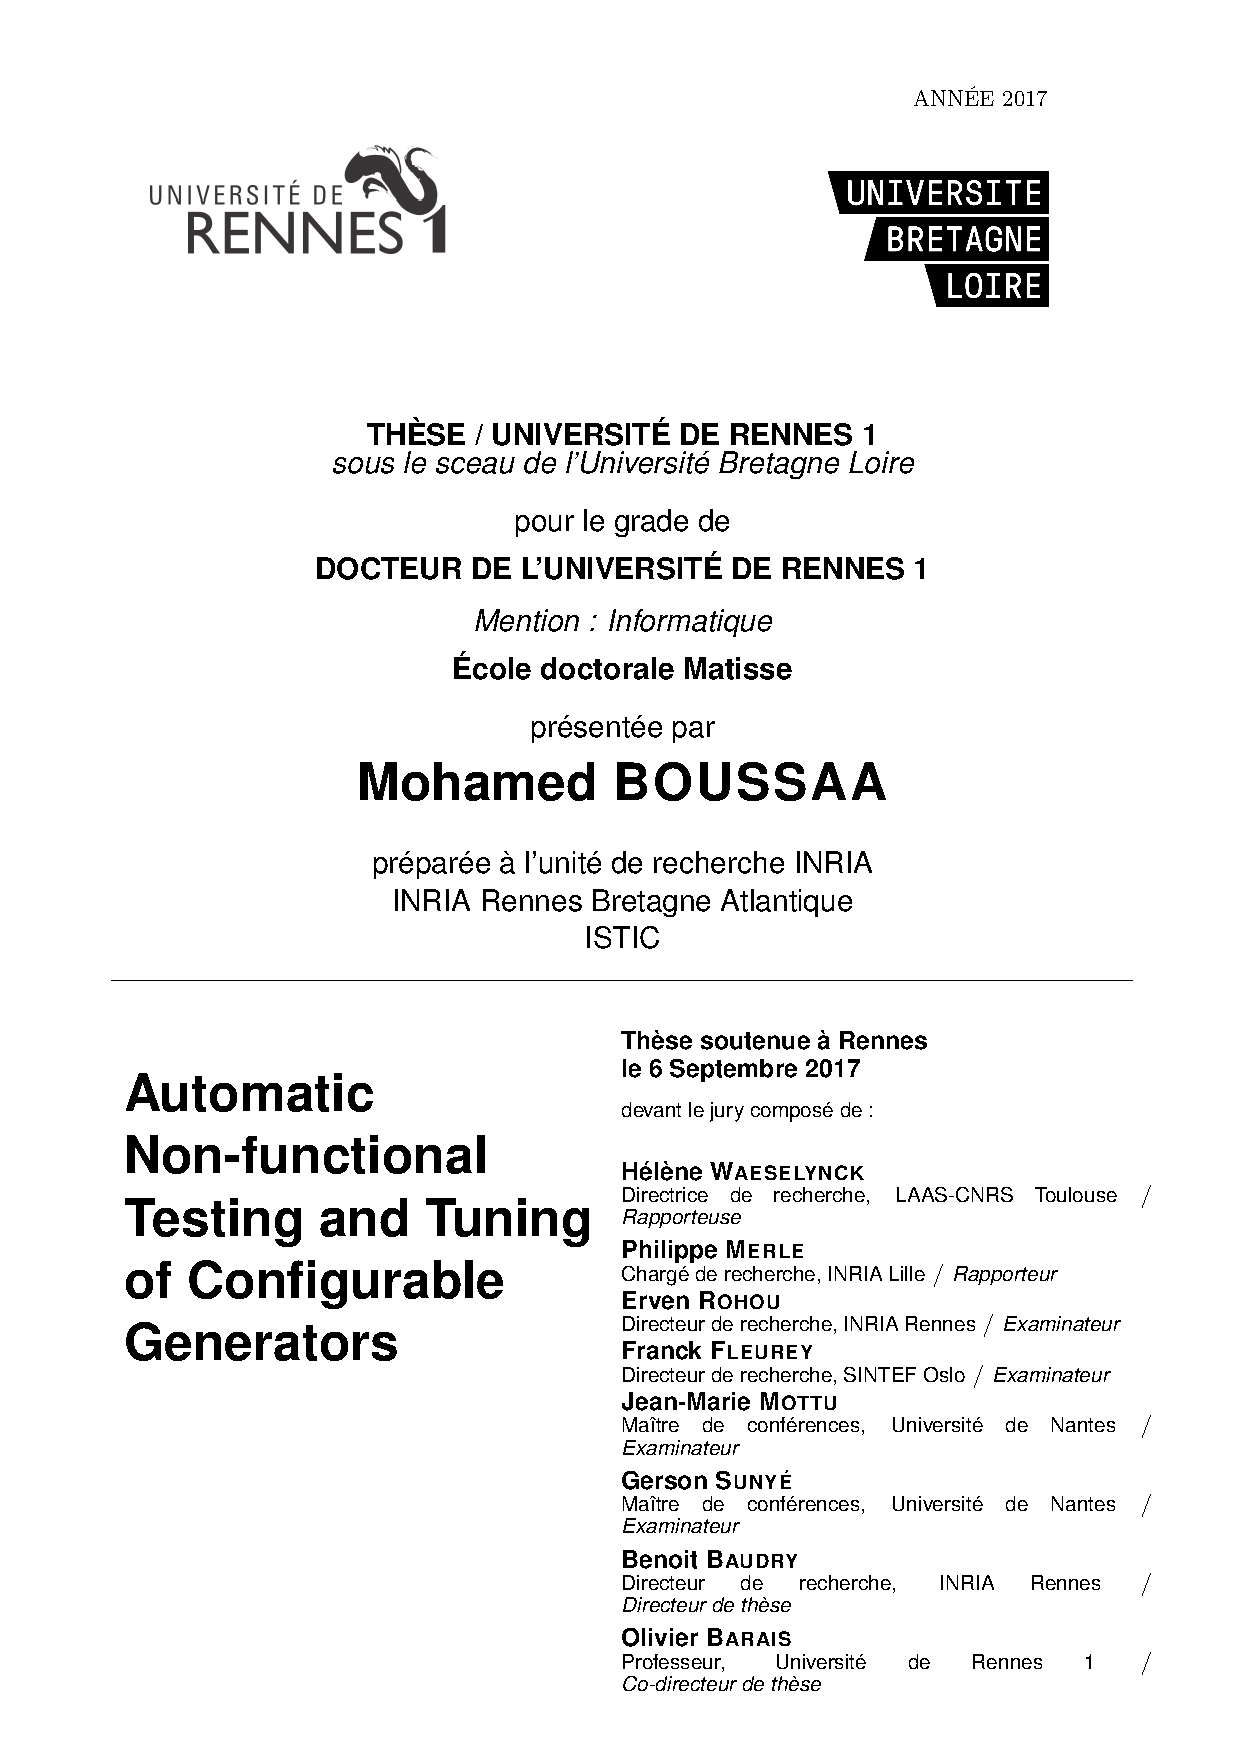
\includepdf{CoverPage/couverture-latex.pdf}

%~\newpage\thispagestyle{empty}\addtocounter{page}{-1}
%~\newpage\thispagestyle{empty}\addtocounter{page}{-1}
~\cleardoublepage


%\remerciements
\frontmatter
%-----------------------
%-----------------------
\chapter*{Acknowledgements}
%-----------------------
%-----------------------
This thesis would not have been completed without the help of others...


%~\newpage\thispagestyle{empty}\addtocounter{page}{-1}
%~\newpage



%~\newpage\thispagestyle{empty}\addtocounter{page}{-1}               
%~\newpage\relax
%~\newpage\thispagestyle{empty}
%\newpage\thispagestyle{empty}\addtocounter{page}{-1}
%\cleardoublepage
%\newpage\thispagestyle{empty}\addtocounter{page}{-1}
%\cleardoublepage

%\fontfamilly{phv}
% For a large document, it is a good idea to divide your thesis
% into several files, each one containing one chapter.
% To illustrate this idea, the "front pages" (i.e., title page,
% declaration, borrowers' page, abstract, acknowledgements,
% dedication, table of contents, list of tables, list of figures,
% nomenclature) are contained within the file "uw-ethesis-frontpgs.tex" which is
% included into the document by the following statement.
%----------------------------------------------------------------------
% FRONT MATERIAL
%----------------------------------------------------------------------
%% T I T L E   P A G E
% -------------------
% Last updated May 24, 2011, by Stephen Carr, IST-Client Services
% The title page is counted as page `i' but we need to suppress the
% page number.  We also don't want any headers or footers.
\pagestyle{empty}
\pagenumbering{roman}

% The contents of the title page are specified in the "titlepage"
% environment.
\begin{titlepage}
        \begin{center}
        \vspace*{1.0cm}

        \Huge
        {\bf University of Waterloo E-Thesis Template for \LaTeX }

        \vspace*{1.0cm}

        \normalsize
        by \\

        \vspace*{1.0cm}

        \Large
        Pat Neugraad \\

        \vspace*{3.0cm}

        \normalsize
        A thesis \\
        presented to the University of Waterloo \\ 
        in fulfillment of the \\
        thesis requirement for the degree of \\
        Master of Science \\
        in \\
        Zoology \\

        \vspace*{2.0cm}

        Waterloo, Ontario, Canada, 2007 \\

        \vspace*{1.0cm}

        \copyright\ Pat Neugraad 2007 \\
        \end{center}
\end{titlepage}

% The rest of the front pages should contain no headers and be numbered using Roman numerals starting with `ii'
\pagestyle{plain}
\setcounter{page}{2}

\cleardoublepage % Ends the current page and causes all figures and tables that have so far appeared in the input to be printed.
% In a two-sided printing style, it also makes the next page a right-hand (odd-numbered) page, producing a blank page if necessary.
 


% D E C L A R A T I O N   P A G E
% -------------------------------
  % The following is the sample Delaration Page as provided by the GSO
  % December 13th, 2006.  It is designed for an electronic thesis.
  \noindent
I hereby declare that I am the sole author of this thesis. This is a true copy of the thesis, including any required final revisions, as accepted by my examiners.

  \bigskip
  
  \noindent
I understand that my thesis may be made electronically available to the public.

\cleardoublepage
%\newpage

% A B S T R A C T
% ---------------

\begin{center}\textbf{Abstract}\end{center}

This is the abstract.

Vulputate minim vel consequat praesent at vel iusto et, ex delenit, esse euismod luptatum augue ut sit et eu vel augue autem feugiat, quis ad dolore. Nulla vel, laoreet lobortis te commodo elit qui aliquam enim ex iriure ea ullamcorper nostrud lorem, lorem laoreet eu ex ut vel in zzril wisi quis. Nisl in autem praesent dignissim, sit vel aliquam at te, vero dolor molestie consequat.

Tation iriure sed wisi feugait odio dolore illum duis in accumsan velit illum consequat consequat ipsum molestie duis duis ut ullamcorper. Duis exerci odio blandit vero dolore eros odio amet et nisl in nostrud consequat iusto eum suscipit autem vero. Iusto dolore exerci, ut erat ex, magna in facilisis duis amet feugait augue accumsan zzril delenit aliquip dignissim at. Nisl molestie nibh, vulputate feugait nibh luptatum ea delenit nostrud dolore minim veniam odio volutpat delenit nulla accumsan eum vero ullamcorper eum. Augue velit veniam, dolor, exerci ea feugiat nulla molestie, veniam nonummy nulla dolore tincidunt, consectetuer dolore nulla ipsum commodo.

At nostrud lorem, lorem laoreet eu ex ut vel in zzril wisi. Suscipit consequat in autem praesent dignissim, sit vel aliquam at te, vero dolor molestie consequat eros tation facilisi diam dolor. Odio luptatum dolor in facilisis et facilisi et adipiscing suscipit eu iusto praesent enim, euismod consectetuer feugait duis. Odio veniam et iriure ad qui nonummy aliquip at qui augue quis vel diam, nulla. Autem exerci tation iusto, hendrerit et, tation esse consequat ut velit te dignissim eu esse eros facilisis lobortis, lobortis hendrerit esse dignissim nisl. Nibh nulla minim vel consequat praesent at vel iusto et, ex delenit, esse euismod luptatum.

Ut eum vero ullamcorper eum ad velit veniam, dolor, exerci ea feugiat nulla molestie, veniam nonummy nulla. Elit tincidunt, consectetuer dolore nulla ipsum commodo, ut, at qui blandit suscipit accumsan feugiat vel praesent. In dolor, ea elit suscipit nisl blandit hendrerit zzril. Sit enim, et dolore blandit illum enim duis feugiat velit consequat iriure sed wisi feugait odio dolore illum duis. Et accumsan velit illum consequat consequat ipsum molestie duis duis ut ullamcorper nulla exerci odio blandit vero dolore eros odio amet et.

In augue quis vel diam, nulla dolore exerci tation iusto, hendrerit et, tation esse consequat ut velit. Duis dignissim eu esse eros facilisis lobortis, lobortis hendrerit esse dignissim nisl illum nulla minim vel consequat praesent at vel iusto et, ex delenit, esse euismod. Nulla augue ut sit et eu vel augue autem feugiat, quis ad dolore te vel, laoreet lobortis te commodo elit qui aliquam enim ex iriure. Ut ullamcorper nostrud lorem, lorem laoreet eu ex ut vel in zzril wisi quis consequat in autem praesent dignissim, sit vel. Dolore at te, vero dolor molestie consequat eros tation facilisi diam. Feugait augue luptatum dolor in facilisis et facilisi et adipiscing suscipit eu iusto praesent enim, euismod consectetuer feugait duis vulputate veniam et.

Ad eros odio amet et nisl in nostrud consequat iusto eum suscipit autem vero enim dolore exerci, ut. Esse ex, magna in facilisis duis amet feugait augue accumsan zzril. Lobortis aliquip dignissim at, in molestie nibh, vulputate feugait nibh luptatum ea delenit nostrud dolore minim veniam odio. Euismod delenit nulla accumsan eum vero ullamcorper eum ad velit veniam. Quis, exerci ea feugiat nulla molestie, veniam nonummy nulla. Elit tincidunt, consectetuer dolore nulla ipsum commodo, ut, at qui blandit suscipit accumsan feugiat vel praesent.

Dolor zzril wisi quis consequat in autem praesent dignissim, sit vel aliquam at te, vero. Duis molestie consequat eros tation facilisi diam dolor augue. Dolore dolor in facilisis et facilisi et adipiscing suscipit eu iusto praesent enim, euismod consectetuer feugait duis vulputate.

\cleardoublepage
%\newpage

% A C K N O W L E D G E M E N T S
% -------------------------------

\begin{center}\textbf{Acknowledgements}\end{center}

I would like to thank all the little people who made this possible.
\cleardoublepage
%\newpage

% D E D I C A T I O N
% -------------------

\begin{center}\textbf{Dedication}\end{center}

This is dedicated to the one I love.
\cleardoublepage
%\newpage

% T A B L E   O F   C O N T E N T S
% ---------------------------------
\renewcommand\contentsname{Table of Contents}
\tableofcontents
\cleardoublepage
\phantomsection
%\newpage

% L I S T   O F   T A B L E S
% ---------------------------
\addcontentsline{toc}{chapter}{List of Tables}
\listoftables
\cleardoublepage
\phantomsection		% allows hyperref to link to the correct page
%\newpage

% L I S T   O F   F I G U R E S
% -----------------------------
\addcontentsline{toc}{chapter}{List of Figures}
\listoffigures
\cleardoublepage
\phantomsection		% allows hyperref to link to the correct page
%\newpage

% L I S T   O F   S Y M B O L S
% -----------------------------
% To include a Nomenclature section
% \addcontentsline{toc}{chapter}{\textbf{Nomenclature}}
% \renewcommand{\nomname}{Nomenclature}
% \printglossary
% \cleardoublepage
% \phantomsection % allows hyperref to link to the correct page
% \newpage

% Change page numbering back to Arabic numerals
\pagenumbering{arabic}

 
 

 
 

 
 
\tableofcontents%%{Table des matières}

 
%%----------------------------%%
%%                            %%
%%  CHAPITRES PRINCIPAUX      %%
%%                            %%
%%----------------------------%%

%======================================================================



%~\newpage\thispagestyle{empty}\addtocounter{page}{-1}               
%~\newpage\relax

\mainmatter

%------------------------------%
%------------------------------%
\chapter*{R\'esum\'e en Fran\c{c}ais}
\addcontentsline{toc}{chapter}{R\'esum\'e en Fran\c{c}ais}
%\addcontentsline{toc}{chapter}{R\'esum\'e en Fran\c{c}ais}
%------------------------------%
%-----------------------------%
\markboth{R\'esum\'e en Fran\c{c}ais}{R\'esum\'e en Fran\c{c}ais}
\section*{Contexte}
\addcontentsline{toc}{section}{Contexte}
\section*{Motivations}
\addcontentsline{toc}{section}{Motivations}
\section*{Probl\'ematique}
\addcontentsline{toc}{section}{Probl\'ematique}
\section*{Contributions}
\addcontentsline{toc}{section}{Contributions}



\chapter{Introduction}


\section{Context}
Modern software systems rely nowadays on a highly heterogeneous and dynamic interconnection of platforms and devices that provide a wide diversity of capabilities and services. These heterogeneous services may run in different environments ranging from cloud servers with virtually unlimited resources down to resource-constrained devices with only a few KB of RAM. Effectively developing software artifacts for multiple target platforms and hardware technologies is then becoming increasingly important. As a consequence, we observe in the last years~\cite{Czarnecki:2000:GPM:345203}, that high-level abstract development received more and more attraction to tame with the runtime heterogeneity of platforms and technological stacks that exist in several domains such as mobile or Internet of Things~\cite{betz2011improving}.

Therefore, software developers tend to increasingly use generative programming~\cite{Czarnecki:2000:GPM:345203} and model-based techniques~\cite{france2007model} in order to reduce the effort of software development and maintenance by developing at a higher-level of abstraction through the use of domain-specific languages (DSLs) for example. 
Consequently, the new advances in hardware and platform specifications have paved the way for the creation of multiple \textit{code generators} and \textit{compilers} that serve as a basis to target different ranges of software platforms and hardware. 

On the one hand, code generators are needed to transform the high-level system specifications (e.g., textual or graphical modeling language) into conventional source code programs (e.g., General-purpose Languages GPLs such as Java, C++, etc). Automatic code generation can of course improve the quality and consistency of a program as well the productivity of software development.
%In general, the generated code has no details about the hardware platform on which the generated machine code will run. 
%For example, the generated application can be executed in a Microsoft Windows environment as a C\# application that interacts with an SQL Server database; or in a Linux environment as a Java application interacting with a MySQL database. 

On the other hand, compilers are also needed to transform the high-level programming language, that was manually written or automatically generated, into low-level machine code (i.e., binaries, executables). 
Compilers bridge the gap between the source code programs (i.e., written using GPLs) and the target execution environment by taking into account different hardware architectures and properties such as register usage, memory organizations, hardware-specific optimizations, etc. 

With full automatic code generation, it is now possible to develop the code easily and rapidly. Nevertheless, it is crucial that the software being automatically generated undergoes an appropriate verification and validation technique to determine that the code generator has generated correct code. Therefore, users can trust the code generator and gain confidence in its correct functioning. Similarly, compilers have to be evaluated and examined in order to ensure that the code they produce is correct.

However, code generators as well as compilers are known to be difficult to understand since they involve a set of complex and heterogeneous technologies and configurations whose complex interdependencies pose important testing challenges. 
%to refactor

For example, when the software developer intends to apply automatic code production, he may create his own code generator or compiler, introducing some optimizations to ensure some non-functional requirements, or he could benefit from the work of others by using and configuring an existing off-the-shelf compiler/code generator. 

Automatically evaluating the quality of produced code (i.e., for the code generator) and choosing the best configuration to apply (i.e., for the compiler) pose many challenges, especially for the non-functional requirements such as the resource usage and execution speed of generated code, the code size, etc.


\section{Motivation}

When an automatic code generator is used, it is important to test if the code generator works properly.
If so, users will trust the code generator and will more likely to continue using it for production code generation. Contrarily, any issue with the generated code leads to a loss of confidence in code generators and users will unlikely continue to use them during software development.
 
Validation of the code generator is principally the tool vendor's responsibility. Code generators users (e.g., customers) are also responsible of this validation since they will continuously report the faults encountered during the automatic code generation. 

For code generator developers, testing the automatic code generation consists on applying a virtuous cycle known as the \textit{"edit, compile, and test"} cycle. 
For example, in case of releasing a new generator version, developers edit the templates and transformation rules that define the code generation process to add new rules and settings, and then generate the output files. These output files are then compiled (or not) and the generated application is executed and tested. At this point, if they find a problem in the generated code, they alter the templates or the input of the generator and re-generate. This cycle is repeated as long as new changes are applied. 
%As an example, in model-driven engineering, a platform-dependent model (PIM) is transformed into a platform specific model (PSM). PIM to PSM translations are done either by hand or by applying automatic model transformation tools. Then code generation is performed from PSM by using some sort of template-based code generator. Generated code is then inspected and augmented by developers. In case of errors the program model, code templates, or implementation platform model are adjusted and program code is generated repeatedly\cite{herrington2003code}. This process iterates until results are satisfactory.

In case of using an off-the-shell code generator during software development (e.g., commercial code generators), users have little control on the behavior and design of code generators which give less freedom to customize/tune the generated code. This is because code generators act generally as a black box where code transformations are internally managed in a very complex way (depending on the nature of the generator model-to-model, model-to-text, text-to-text transformation rules, etc).
However, they do have more control on the structure and design of the input high-level language or model. 
Hence, to test code generators, users (i.e., software developers) have to write a well-designed program supported by the generator (e.g., DSL, Model, GPL, etc). Afterwards, they apply automatic code transformations by generating code to the target programming language. In this case, since the generator is not editable, the quality of the generated code depends only on the efficiency of the selected code generator for the target platform. So, testing code generators is mainly to find coding errors at the source code level. If they find any issues with the generated code, the bugs are reported to the generator suppliers in order to fix them (e.g., add documentation, add typing support, etc.).
For example, this is widely used in the industry by applying the concept of "write once, run everywhere" where users can benefit from a family of code generators (e.g., cross-platform code generators\cite{fumero2015runtime}) to generate from the manually written (high-level) code different implementations of the same program in different languages. This technique is very useful to address diverse software platforms and programming languages.





Unlike code generators, compilers, nowadays, are more user-friendly and highly configurable\cite{fursin2008milepost}. Thus, the generated executables can be easily customized to satisfy the user requirements. Indeed, compilers such as GNU compilers and LLVM provide a large selection of configuration options to control the compiler behavior. For example, different categories of options can be enabled (i.e., option flags) to help developers to: debug their applications, optimize and tune application performance, select language levels and extensions for compatibility, select the target hardware architecture, and perform many other common tasks that configure the way executables are generated.
%These compiler options can be enabled through a combination of environment variables, compiler configuration files, command line options, and plugins. 
The huge number of compiler configurations, versions, optimizations and debugging utilities make the task of choosing the best configuration set very difficult and time-consuming. As an example, GCC version 4.8.4 provides a wide range of command-line options that can be enabled or disabled by users, including more than 150 options for optimization. This results in a huge design space with $2^{150}$ possible optimization combinations that can be enabled by the user. In addition, constructing one single optimization sequence that improves the performance or resource usage for all programs is impossible since the interactions between optimizations is too complex and difficult to define. As well, the optimization's impact is highly dependent on the hardware and the input source code.


%there is no only one set of optimizations that will work for all programs. It highly depends on the hardware architecture and the input program.
This example shows how painful it is for the compiler users to tune compilers (through optimization flags) in order to satisfy different non-functional properties such as execution time, compilation time, code size, etc.


The huge design space of compiler configuration options as well as the complexity of code generators make the activities of design, implementation, and testing very hard and time-consuming\cite{guana2015developers}.
From the user's point of view, compilers and code generators are black box components that are used to ease the software production process. The quality of the generated software by either compilers or code generators is directly correlated to the quality of the code generator. As long as the quality of code generators is maintained and improved, the quality of generated software artifacts also improves. Any bug with these generators impacts on the software quality delivered to the market and results in a loss of confidence on the end users.
%Testing code generators consists, in general, on verifying the behavior of generated code. 
As a consequence, generators testers check the correctness of generated source code or binaries with almost the same, expensive effort as it is needed for manually written code. 
Testing code generators and/or correctly tuning compilers is crucial and necessary to guarantee that no errors are incorporated by inappropriate modeling or by the compiler itself.
Faulty code generators or compilers can generate defective software artifacts which range from uncompilable or semantically dysfunctional code that causes serious damage to the target platform; to non-functional bugs which lead to poor-quality code that can affect system reliability and performance (e.g., high resource usage, high execution time, etc.). 
Numerous approaches have been proposed\cite{stuermer2007systematic,yang2011finding} to verify the functional outcome of generated code. However, there is a lack of solutions that pay attention to evaluate the properties related to the performance and resource usage of produced code.


\section{Scope of the thesis}

In this thesis, we seek to test and evaluate the properties related to the resource usage of generated code. 

On the one hand, since many different software platforms can be targeted by the code generator, we provide facilities to the code generator creators and users to monitor the execution of generated code for different targets and have a deep understanding of its non-functional behavior in terms of resource usage. Consequently, we automatically detect the non-functional inconsistencies caused by some faulty code generators. 

On the other hand, we provide a mechanism that helps compiler users to select the best optimization sets that satisfy specific resource usage requirements for a broad range of programs and hardware architectures.

This thesis addresses three problems: 
	
	(1) \textbf{The problem of non-functional testing of code generators:} We benefit from the existence of code generator families to test the automatically generated code. In fact, our proposed approach is based on the metamorphic testing paradigm to detect inconsistencies in code generators families by defining high-level test oracles (i.e., metamorphic relations). We focus in this contribution on the test of the performance and resource usage properties (e.g., intensive resource usage)
	
	(2) \textbf{The problem of compilers auto-tuning:}  We benefit from recent advances in search-based software engineering in order to provide an effective approach to explore the large optimization search space and automatically tuning compilers according to user's non-functional requirements, namely performance and resource usage properties.

	(3) \textbf{The problem of software platforms diversity and heterogeneity in software testing:} To handle this problem, we benefit from the recent advances in lightweight system virtualization, in particular container-based virtualization, in order to offer effective support for deploying, executing, and monitoring of automatically (or not) generated code in heterogeneous environment, based on containers.

In this thesis, we use the term \textbf{"compilers"} to refer to the traditional compilers that take as input a source code and translate it into machine code like GCC, LLVM, ect. Similarly, \textbf{"Code generators"} designate the software programs that transform an input program into source code like JAVA, C++, etc. As well, we use the term \textbf{"generators"} to designate both, code generators and compilers. 

\section{Challenges}
%Due to new advances in hardware and system specification, creating an effective code generators (including compilers) is not simple and it is becoming more and more challenging.
In existing solutions that aim to test code generators and auto-tune compilers, we find three important challenges. Addressing these challenges, which are described below, is the objective of the present work.
\begin{itemize}
\item
\textbf{Code generators testing: the oracle problem:} One of the most common challenges in software testing is the oracle problem. A test oracle is the mechanism by which a tester can determine whether a program has failed or not.
When talking about the non-functional testing of generators, this problem becomes more challenging because it is quite hard to determine the expected output of a generator under test (e.g., memory consumption of the generated program). Determining whether these non-functional outputs correspond to a generator anomaly or not is also not obvious. That is why testing the generated code becomes very complex when the software user has no precise definition of the oracle he would define. 
To alleviate the test oracle problem, techniques such as metamorphic testing\footnote{\url{https://en.wikipedia.org/wiki/Metamorphic_testing}} are widely used to test programs without defining an explicit oracle. Instead, it employs high-level metamorphic relations to verify the outputs automatically.
So, which kind of test oracles can we define? How can we automatically detect inconsistencies? All these questions pose important challenges in testing generators.

\item
\textbf{Auto-tuning compilers: exploring the large optimizations search space:} The current innovations in science and industry demand ever-increasing computing resources while placing strict requirements on many non-functional properties such as system performance, power consumption, size, reliability, etc. In order to deliver satisfactory levels of performance on different processor architectures, compiler creators often provide a broad collection of optimizations that can be applied by compiler users in order to improve the quality of generated code. However, to explore the large optimization space, users have to evaluate the effect of optimizations according to a specific performance objective/trade-off. Thus, constructing a good set of optimization levels for a specific system architecture/target application becomes challenging and time-consuming problem. Due to the complex interactions and the unknown effect of optimizations, users find difficulties to choose the adequate compiler configuration that satisfies a specific non-functional requirement.

\item
\textbf{Runtime monitoring of generated code: handle the heterogeneity of execution platforms and hardwares:} To evaluate the properties related to the resource usage of the generated code (by compilers or code generators), developers generally use to compile, deploy and execute the generated software artifacts on different execution platforms. Then, they have to collect and compare the information about the performance and efficiency of the generated code. Afterwards, they report issues related to the code generation process such as incorrect typing, memory management leaks, etc.
Currently, there is a lack of automatic solutions to check the performance issues such as the inefficiency (high memory/CPU consumption) of the generated code. In fact, developers often use manually several platform-specific profilers, debuggers, and monitoring tools\cite{guana2014chaintracker,delgado2004taxonomy} in order to find some inconsistencies or bugs during code execution. Ensuring the quality of the generated code in this case can refer to several non-functional properties such as code size, resource or energy consumption, execution time, among others\cite{pan2006fast}. Due to the heterogeneity of execution platforms and hardwares, collecting information about the resource usage of generated code becomes very hard and time-consuming task since developers have to analyze and verify the generated code for different target platforms using platform-specific tools. 

%while satisfying all the non-functional requirements for a broad range of programs and architectures

\end{itemize}
The challenges this research tackle can be summarized in the following research questions. These questions arise from the analysis of the challenges presented in the previous paragraphs.

\textit{RQ1.} How can we help code generator suppliers/users to automatically detect non-functional inconsistencies in code generators?

\textit{RQ2.} How can we help compiler users to automatically choose the adequate compiler configuration that satisfies a specific non-functional requirement?

\textit{RQ3.} How can we provide efficient support for resource consumption monitoring and management?


\section{Contributions}
This thesis establishes three core contributions. They are briefly described in the rest of this section.

\textbf{Contribution I: Automatic detection of inconsistencies in code generators families.}
In this contribution, we tackle the oracle problem in the domain of code generators testing. Thus, we propose an approach for automatically detecting inconsistencies in code generator families.
This approach is based on the intuition that a code generator is often a member of a family of code generators. The availability of multiple generators with comparable functionality enables us to apply the idea of metamorphic testing\cite{zhou2004metamorphic} by defining high-level test oracles to detect code generator issues.
We evaluate our approach by analyzing the performance of Haxe, a popular high-level programming language that involves a set of cross-platform code generators. We evaluate the properties related to the resource usage and performance for five different target software platforms. Experimental results show that our approach is able to detect some performance inconsistencies that reveal real issues in this family of code generators.
%In particular, we show that we could find two kinds of errors during code transformation: the lack of use of a specific function and an abstract type that exist in the standard library of the target language which can reduce the memory usage/execution time of the resulting program.

\textbf{Contribution II: Compiler auto-tuning according to the non-functional requirements.}
As we stated earlier, the huge number of compiler options requires the application of a search method to explore the large design space. Thus, we apply, in this contribution, a search-based meta-heuristic called \textit{Novelty search} for compiler optimizations exploration. This approach helps compiler users to effectively auto-tune compilers according to the performance and resource usage properties and that for a specific hardware architecture. 
We evaluate the effectiveness of our approach by verifying the optimizations performed by the GCC compiler.
Our experimental results show that our approach is able to auto-tune compilers according to the user requirements and construct optimizations that yield to better performance results than standard optimization levels. We also demonstrate that our approach can be used to automatically construct optimization levels that represent optimal trade-offs between multiple non-functional properties such as execution time and resource usage requirements.

\textbf{Contribution III: A microservice-based infrastructure for runtime deployment and monitoring of generated code.}
Finally, we propose a micro-service infrastructure to ensure the deployment and monitoring of the different variants of generated code. This contribution addresses the problem of software and hardware heterogeneity. Thus, we describe an approach that automates the process of code generation, compilation, optimization, deployment, execution, and monitoring in order to provide to software developers more facilities to evaluate the quality generated code. 
This isolated and sand-boxing environment is based on system containers, as execution platforms, to provide a fine-grained understanding and analysis of the properties related to the resource usage (CPU and memory). 
This approach constitutes the playground for testing and evaluating the generated code from either compilers or code generators. This contribution answers mainly \textit{RQ3} but the same infrastructure is particularly used to validate the carried experiments in \textit{RQ1} and \textit{RQ2}.

\section{Overview of this thesis}
The remainder of this thesis is organized  as follows:

\textbf{Chapter 2} first contextualizes this research, situating it in the domain of generative programming. We give a background about the different concepts involved in the field of generative programming as well as an overview of the different aspects of automatic code generation in software development. Finally, we discuss the different problems that make the task of compiler auto-tuning and code generators testing very difficult.

\textbf{Chapter 3} presents the state of the art regarding our approach. This chapter provides a survey of the most used techniques for testing compilers and code generators. We focus more on the non-functional testing aspects.
This chapter is divided on two parts. First, we study the previous approaches that have been applied for auto-tuning compiler. Second, we study the different techniques used to test the functional and non-functional properties of code generators. Finally, we discuss the limitations of the state of the art for these both domains.

\textbf{Chapter 4} presents our approach for the non-functional testing of code generators. It shows an adaptation of the idea of metamorphic testing for detecting code generator issues. We report the results of testing multiple generators with comparable functionalities (a code generator family). The non-functional metrics we are evaluating in this section are the performance and memory usage of generated code. We also report the issues we have detected and we propose solutions for code generation improvement.

\textbf{Chapter 5} resumes our contribution for compiler auto-testing. Thus, we present an iterative process based on a search technique called Novelty search for compiler optimizations exploration. We provide two adaptations of this algorithm: mono and multi objective search. We also show how this technique can easily help compiler users to efficiently generate and evaluate the compiler optimizations. The non-functional metrics we are evaluating are the performance, memory and CPU usage. We evaluate this approach through an empirical study and we discuss the results.

\textbf{Chapter 6} shows the testing infrastructure used across all experiments. It shows the usefulness of such architecture, based on system containers, to automatically deploy and execute the generated code by either compilers or code generators. 
We evaluate our infrastructure by comparing it to a non-containerized solution. We report the comparison results between both solutions in terms of overhead and we discuss the results. We also provide a case study to show the automatic monitoring process. 

\textbf{Chapter 7} draws conclusions and identifies future work and perspectives for testing code generators and auto-tuning compilers.

\section{Publications}

\begin{itemize}
	
	\item Mohamed Boussaa, Olivier Barais, Gerson Suny\'e, Beno\^it Baudry:
	\textbf{Automatic Non-functional Testing of Code Generators Families}. In
	\textit{The 15th International Conference on Generative Programming: Concepts \& Experiences (GPCE 2016)},
	Amsterdam, Netherlands, October 2016.

	\item Mohamed Boussaa, Olivier Barais, Beno\^it Baudry, Gerson Suny\'e:
	\textbf{NOTICE: A Framework for Non-functional Testing of Compilers}. In 
	\textit{2016 IEEE International Conference on Software Quality, Reliability \& Security (QRS 2016)}, Vienna, Austria, August 2016.
	
	\item Mohamed Boussaa, Olivier Barais, Gerson Suny\'e, Beno\^it Baudry:
	\textbf{A Novelty Search-based Test Data Generator for Object-oriented Programs}. In 
	\textit{Genetic and Evolutionary Computation Conference Companion (GECCO 2015)}, 
	Madrid, Spain, July 2015.
	
	\item Mohamed Boussaa, Olivier Barais, Gerson Suny\'e, Beno\^it Baudry:
	\textbf{A Novelty Search Approach for Automatic Test Data Generation}. In
	\textit{8th International Workshop on Search-Based Software Testing (SBST@ICSE 2015)}, 
	Florence, Italy, May 2015.

	
	
\end{itemize}



\part{Background and State of the Art}
\chapter{Background}
 
In this chapter, the context of this thesis and the general problems it faces are introduced. The objective of this chapter is to give a brief introduction to  different domains and concepts in which our work takes place and used throughout this document.
This includes an overview of the generative software development process as we see in the context of this thesis, the main actors and their roles for tuning and testing configurable generators, and the main challenges we are facing.

 %It aims at providing a better understanding of the background and context in which our work takes place, as well as the terminology and concepts presented in the next chapters.

The chapter is structured as follows: 

In Section~\ref{bg:Diversity in software engineering}, we present the problem of software diversity and hardware heterogeneity caused by the continuous innovation in science and technology.

Section~\ref{sec:FROM} aims at providing a better understanding of the generative programming concept. We present the different steps of automatic code generation involved during software development as well as the different stakeholders and their roles in testing and tuning generators. We highlight then, the main activities that the software developer goes through from the software design until the release of the final software product.

Section~\ref{bg:Testing code generators} gives an overview of the different types of code generators used in the literature and we show the complexity of testing code generators.

Similarly, in Section~\ref{bg:Compilers auto-tuning}, we describe some compiler optimizations and we illustrate the compiler auto-tuning complexity by presenting the different challenges that this task is posing.

Finally, in Section~\ref{bg:Summary: Testing and optimization challenges}, we conclude by providing a summary of the relevant challenges for testing and tuning configurable generators.

\section{Diversity in software engineering}
\label{bg:Diversity in software engineering}
%context
The history of software development shows a continuous increase of complexity in several aspects of the software development process. This complexity is highly correlated with the actual technological advancement in the software industry as more and more heterogeneous devices are introduced in the market~\cite{betz2011improving}. 
Generally, heterogeneity may occur in terms of different system complexities, diverse programming languages and platforms, types of systems, development processes and distribution among development sites\cite{ghazi2015heterogeneous}.
%System heterogeneity we are discussing in this thesis is the software and hardware diversity.
System heterogeneity is often led by software and hardware diversity.
Diversity emerges as a critical concern that spans all activities in software engineering, from design to operation\cite{acher2014software}. It appears in different areas such as mobile, web development\cite{doukas2013compose}, security\cite{allier2015multitier}, etc.

However, software and hardware diversity leads to a greater risk for system failures due to the continuous change in configurations and system specifications.
As a matter of a fact, effectively developing software artifacts for multiple target platforms and hardware technologies is then becoming increasingly important.
Furthermore, the increasing relevance of software and the higher demand in quality and performance contribute to the complexity of software development.

In this background introduction, we discuss two different dimensions of diversity: (1) software diversity, and (2) hardware heterogeneity.

%The history of software development shows a continuous increase of complexity in several aspects of the software development process~\cite{betz2011improving}. 
%Diversity
 
 
%problem
%Furthermore, the increasing relevance of software in general and the higher demand in quality and performance contribute to the complexity of software development. 
%Today, softwares and services are running everywhere. These services are running on top of heterogeneous software and hardware platforms.
\subsection{Hardware heterogeneity}
\label{sec:Hardware diversity}
Modern software systems rely nowadays on a highly heterogeneous and dynamic interconnection of devices that provide a wide diversity of capabilities and services to the end users.
These heterogeneous services run in different environments ranging from cloud servers to resource-constrained devices.
Hardware heterogeneity comes from the continuous innovation of hardware technologies to support new system configurations and architectural design (\eg, addition of new features, a change in the processor architecture, new hardware is made available, etc). 
For example, until February 2016\footnote{\url{https://arstechnica.com/information-technology/2016/02/moores-law-really-is-dead-this-time/}}, the increase in capacity of microprocessors has followed the famous Moore's law\footnote{\url{https://en.wikipedia.org/wiki/Moore\%27s_law}} for Intel processors. Indeed, the number of components (transistors) that can be fitted onto a chip doubles every two years, increasing the performance and energy efficiency.
For instance, Intel Core 2 Duo processor was introduced in 2006 with 291 millions of transistors and 2.93 GHz clock speed. Two years later, Intel has introduced the Core 2 Quad processors which came up with 2.66 GHz clock speed and the double number of transistors introduced in 2006 with 582 millions of transistors.

In the last years, modern processors becomes more and more heterogeneous, using more than one kind of processor or cores, called ``co-processors''. The CPU can even use different instruction set architectures (ISA), where the main processor has one and the rest have another, usually a very different architecture. Operations performed by the co-processor may be floating point arithmetic, graphics, signal processing, string processing, encryption or I/O Interfacing with peripheral devices. 
As an example, the ARM big.Little processor architecture\footnote{\url{https://en.wikipedia.org/wiki/ARM_big.LITTLE}} released in 2011 (see Figure \ref{fig:cortex}), is a power-optimization technology where high-performance ARM CPU cores are combined with the most efficient ARM CPU cores to deliver peak-performance capacity and increased parallel processing performance, at significantly lower average power. It can save 75\% of CPU energy and can increase performance by 40\% in highly threaded workloads.
The intention of this architecture is to create a multi-core processor that can adjust better to dynamic computing needs.
Threads with high priority or computational intensity can in this case be allocated to the ``Big'' cores while threads with less priority or less computational intensity, such as background tasks, can be performed by the ``Little'' cores. This model has been implemented in the Samsung Exynos 5 Octa in 2013\footnote{\url{http://www.embedded.com/electronics-news/4419448/Benchmarking-ARM-s-big-little-architecture}}.


\begin{figure}[h]
	\center
	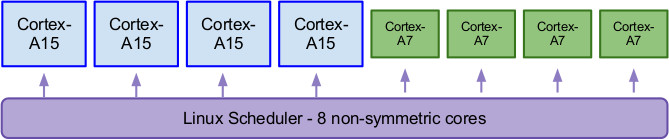
\includegraphics[scale=0.7]{Background/fig/cortex.jpg}
	\caption{ARM Big.Little heterogeneous multi-processing}
	\label{fig:cortex}
\end{figure}


Given the complexity of new emerging processors architecture (x86, x64, multi-core, etc) and CPU manufacturers such as ARM, AMD, and Intel, some of the questions that developers have to answer when facing hardware heterogeneity: 
Is it easy to deliver satisfactory levels of performance on modern processors? How is it possible to produce machine code that can exploit efficiently the continuous hardware changes? 





%Which optimizations are applied by compiler users in order to satisfy  the non-functional properties of a broad range of programs and hardware architectures such as energy consumption, execution time, etc. 


%end 


%Model-Driven Software Engineering and generative programming techniques to provide a new integrated software engineering approach which enables the advanced exploitation of the full range of diversity and specificity of the future computing continuum

%Diversity increases system complexity and leads to a greater risk for system failures. Efficient validation and verification methods are, thus, essential to guarantee qualities of diverse systems, such as security, consistency, correctness or performance

\subsection{Software diversity}
\label{sec:Software diversity}
In today's software systems, different software variants are typically developed simultaneously to address a wide range of application contexts and customer requirements\cite{schaefer2012software}. 
Therefore, software is built using different approaches and languages, depending on the application domain.

In the literature, Baudry \etal\cite{baudry2015multiple} and Schaefer \etal\cite{schaefer2012software} have presented an exhaustive overview of the multiple facets of software diversity in software engineering. 
According to their study, software diversity can emerge in different types and dimensions such as diversity of operating systems, programming languages, data structures, components, execution environments, etc. 
Like all modern software systems, software need to be adapted to address changing requirements over time supporting system evolution, technology and market needs like considering new software platforms, new languages, new customer choices, etc.

In order to understand the skills and capabilities required to develop software on top of different classes of devices and application domains, we queried a popular open-source repository \textit{GitHub} to evaluate the diversity of existing programming languages.  
The following sets of keywords were used: \textit{1) Cloud:} server with virtually unlimited resources, \textit{2) Microcontroller:} resource constrained node (few KB RAM, few MHz),  \textit{3) Mobile:} an intermediate node, typically a smartphone,  \textit{4) Internet of Things:} Internet-enabled devices,  \textit{5) Cyber Physical System}, and  \textit{6) Embedded systems}, as a large and important part of the service implementations will run as close as possible to physical world, embedded into sensors, devices and gateways.

\begin{figure}[h]
	\center
	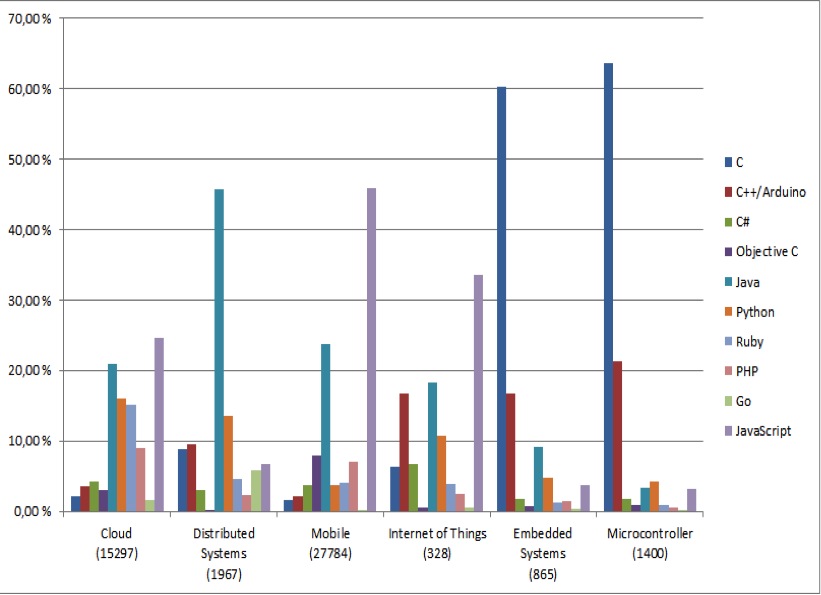
\includegraphics[scale=1.]{Background/fig/github}
	\caption{Popularity of 10 programming languages in different application domains}
	\label{fig:github}
\end{figure}

Figure \ref{fig:github} presents the results of those queries. The queried keywords are presented on the \textit{x-axis} together with the number of matches for that keyword. For each keyword, the \textit{y-axis} represents the popularity (in per cent of the total number of matches) of each of the 10 most popular programming languages that we encountered.


This simple study indicates that no programming language is popular across the different areas. A general trend indicates that Java and JavaScript (and to some extent, Python and Ruby) are popular in cloud and mobile, whereas C (and to some extent, C++) is a clear choice for developers targeting embedded and microcontroller-based systems. Other languages do not score more 10\% for any of the keywords. 
For all keywords except Cloud, the combined popularity of Java, JavaScript and C/C++ (\ie, the sum
of the percentages) is above 70\%. For Cloud, we observe a large use of Python, Ruby also being very popular, so the combined popularity of Java, JavaScript and C/C++ is only 50\%. It is also worth noticing that the most popular language for a given keyword scores very poorly (less than 5\%) for at least another keyword. While it might appear that a combination of C/C++, JavaScript and Java should be able to cover all the areas, in practice it does not exclude the need for other programming languages. For example, the Fibaro Home Center 2 (a gateway for home automation based on the Z-Wave protocol) uses Lua as scripting language to define automation rules. Another example is the BlueGiga BlueTooth Smart Module, which can be scripted using BGScript, a proprietary scripting language. This shows that each part of an infrastructure might require the use of a niche language, middleware or library to be exploited to its full potential.


In summary, the variation of programming languages for the different kinds of devices and application domains induces a high \textit{software diversity}. Accordingly, we propose the following definition of software diversity in the context of this thesis: 
\textit{Software diversity is the generation or implementation of the same program specification in different ways/manners in order to satisfy one or more diversity dimensions such as the diversity of programming languages, execution environments, functionalities, etc. }
		
%We define as well the term \textbf{"software family"} to categorize these diverse programs that share commonalities. 

%The key concept of code generators is to produce code in a general-purpose language, such as Java or C++, that can be compiled and executed. Target execution platforms of the generated code are heterogeneous and diverse.



\subsection{Matching software diversity to heterogeneous hardware: the marriage}
\subsubsection{Challenges}
The hardware and software communities are both facing significant change and major challenges. Figure~\ref{fig:marriage} shows an overview of the challenges that both communities are facing. In fact, hardware and software are pulling us in opposite directions. 

\begin{figure}[h]
	\center
	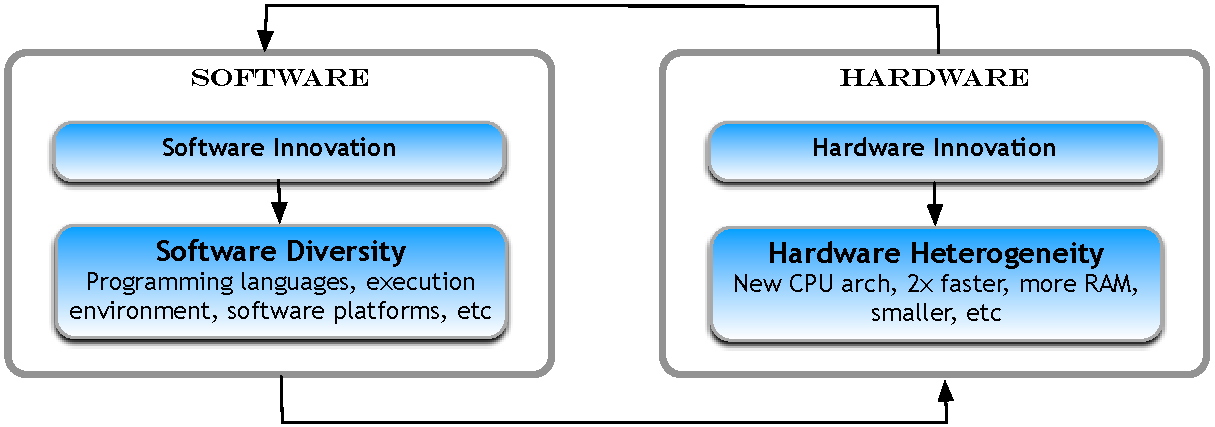
\includegraphics[scale=0.65]{Background/fig/marriage}
	\caption{Matching software to hardware}
	\label{fig:marriage}
\end{figure}


On the one hand, software is facing challenges of a similar magnitude, with major changes in the way software is deployed, is sold, and interacts with hardware. 
Software diversity, as discussed in Section~\ref{sec:Software diversity}, is driven by software innovation, driving the software development toward highly configurable and complex systems. This complexity is carried by the huge diversity of software technologies, customer configurations, execution environments, programming languages, etc. This explosion of configurations that software is facing makes the activity of testing and validation very difficult and time consuming. 
As a consequence, software becomes higher and higher level, managing complexity and gluing lot of pieces together to give programmers the right abstraction for how things really work and how the data is really represented. 


On the other hand, hardware is exposing us to more low-level details and heterogeneity due to the continuous hardware innovation. 
Hardware innovation offers us energy efficiency, performance improvement but exposes a lot of complexity for software engineers and developers.
For example, in~\cite{he2010computer}, authors argue that system software is not ready for this heterogeneity and cannot fully benefit from new hardware advances such as multi-core and many-core processors. Although multi-core processors have been used in everyday life, we still do not know how to best organize and use them. 
Meanwhile, hardware specialization for every single application is not a sustainable way of building chips.
%So, what the software community can do to address/deal with devices heterogeneity? How hardware innovation can be exploited in the software?

%\paragraph{So how can we match software diversity to heterogeneous hardware?}~\\ 
\subsubsection{Mapping software to hardware}
\label{Mapping software to hardware}
Matching software to hardware is ensured by the efficient translation of the high-level software programs into a machine code that better exploit the hardware changes (relation 1 in Figure~\ref{fig:marriage}). This is exactly what a compiler is intended to do.

\paragraph{Configuring existing compilers}~\\ 
Well, gone are the days where we used to write the assembly code by hand and from scratch. Now, it is up to the compilers to handle this heterogeneity and to efficiently generate and optimize the code for a particular microprocessor. 

As shown in Figure~\ref{fig:compilers}, a compiler is typically divided into two parts, a front-end and a back-end. The compiler front-end verifies the syntax and semantics and analyzes the source code to build an internal representation of the program, called the intermediate representation or IR. For example, the GNU Compiler Collection (GCC) and LLVM support many front-ends with programming languages such as C, C++, Objective-C, Objective-C++, Fortran, Java, Ada, and Go, among others. The compiler back-end generates the target-dependent assembly code and performs optimizations for the target hardware architecture. Typically, the output of a back-end is a machine code specialized for a particular processor and operating system (\eg, ARM, Sparc processors, etc).
As a consequence, people who are writing compilers have to continuously enhance the way these executables are produced by releasing new compiler versions to support new hardware changes (\ie, introducing new optimization flags, instruction sets, etc.). 
\begin{figure}[h]
	\center
	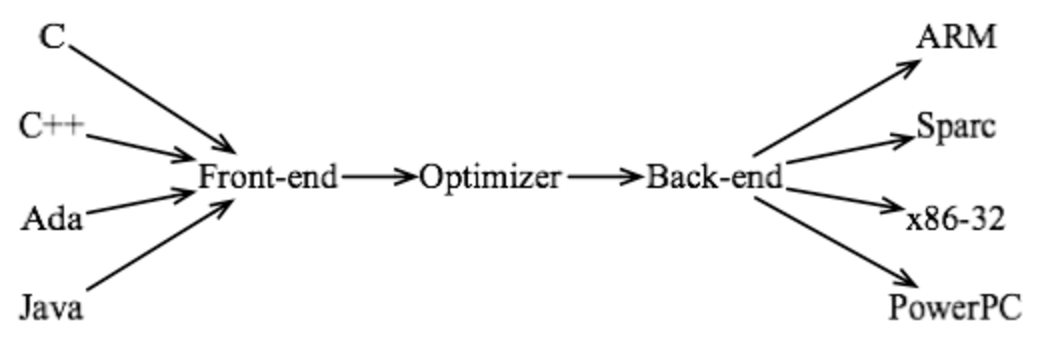
\includegraphics[scale=0.65]{Background/fig/compilers}
	\caption{Compiler architecture}
	\label{fig:compilers}
\end{figure}

Let's take the GCC example. GCC is able to generate code automatically for approximately \textbf{more than 40 different processor architectures}. Hence, GCC becomes highly configurable, allowing the compiler user to enable multiple flags to customize the generated code. For instance, one important compiler flag is \textit{-march}. It tells the compiler what code it should produce for the system's processor architecture. It tells GCC that it should produce code for a certain kind of CPU. Using \textit{-march=native} enables all the optimization flags that are applicable for the native system's CPU, with all its capabilities, features, instruction sets, and so on. There exits many other configuration options for the target CPU like \textit{--with-arch=i7}, \textit{--with-cpu=corei7}, etc.
Generally, each time a new family of processors is released, compiler developers release a new compiler version with more sophisticated configuration options for the target platform. For example, old compilers produce only 32-bit programs. These programs still run on new 64-bit computers, but they may not exploit all processor capabilities (\eg, they will not use the new instructions that are offered by x64 CPU architecture). For instance, the current x86-64 assembly language can still perform arithmetic operations on 32-bit registers using instructions like addl, subl, andl, orl, etc, with the l standing for ``long'', which is 4 bytes/32 bits. 64-bit arithmetic is done with addq, subq, andq, orq, etc, with q standing for ``quadword'', which is 8 bytes/64 bits.

Another example is that compilers need to support parallelism. In fact, we can see that modern computers today can do many things at once and modern CPUs becomes highly parallel processors with different levels of parallelism (\eg, the ARM Big.Little in Figure~\ref{fig:cortex}). We find parallelism everywhere from the parallel execution units in a CPU core, up to the SIMD (Single Instruction, Multiple Data) instruction set and the parallel execution of multiple threads.  One of the commonly applied optimizations by modern compilers in parallel computing is vectorization. It constitutes the process of converting an algorithm from a scalar implementation, which processes a single pair of operands at a time, to a vector implementation, which processes one operation on multiple pairs of operands at once.
Programmers can exploit vectorization using compilers to speedup certain parts of their code. One hot research topic in computer science is the search for methods of automatic vectorization\cite{nuzman2006auto}: seeking methods that would allow a compiler to convert scalar algorithms into vectorized algorithms without human intervention.


In short, to cope with heterogeneous hardware platforms, software developers use these highly configurable compilers (for compiled languages such as C or C++) in order to efficiently compile their high-level source code programs and execute them on top of a board range of platforms and processors. 


\paragraph{Masking hardware heterogeneity}~\\ 
Sometimes, software developers try to avoid the hardware heterogeneity. Thus, they use for example managed languages such as Java, Scala, C\#, etc to favor software portability. Instead of compiling to native machine instruction set, these languages are compiled into an intermediate language or IL, which is similar to a binary assembly language. These instructions are executed by a JVM, or by .NET's CLR virtual machine, which effectively translates them to native binary instructions specific to the CPU architecture and/or OS of the machine.
By using managed code, memory management such as a garbage collector, type safety checking, and destruction of unneeded objects are handled internally within this sandbox runtime environment. Thus, developers focus on the business logic of applications to provide more secure and stable software without taking too much care of the hardware heterogeneity.
However, using managed languages has drawbacks. It includes slower startup speed (the managed code must be JIT compiled by the VM). It can also be slower than native code and generally more greedy in terms of system resources. 
For example, we can see in Figure~\ref{fig:github}, that the C language is the most widely used programming language in the context of embedded systems\footnote{\url{http://www.eetimes.com/author.asp?doc_id=1323907}} where the system is really resource-constrained. Contrarily to managed languages, C utilizes the hardware to its maximum by multi-processing and multi-threading APIs provided by POSIX. It also controls the memory management and uses less memory (which allows more freedom on memory management compared to the use of garbage collector).   


\paragraph{Building new DSLs and compilers}~\\ 
An alternative approach for matching software to hardware is to build new languages and compilers for a specific domain from scratch. 
For example, Hou \etal\cite{hou2010spap} have presented a container-based programming language for heterogeneous many-core systems. This DSL allows programmers to write unified programs that are able to run efficiently on heterogeneous processors. To map this DSL to such hardware processors, they provide a set of compilers and runtime environments for the x86 CPUs
and CUDA GPUs. Similarly, Chafi \etal\cite{chafi2010language,chafi2011domain} proposed leveraging DSLs to map high-level application code to heterogeneous devices. Results show that the presented DSL can achieve high performance on heterogeneous parallel hardware with no modification required to the source code. They compared this language performance to MATLAB code and they showed that it outperformed it in nearly all cases.

%In contrast, devices in turn, may impose the support of specific programming languages (relation 2 in Figure \ref{fig:marriage}). 
%In mobile development for example, Java is needed to implement Android applications and Objective-C is needed to develop iOS products. This means that developers need to create multiple clients in this heterogeneous environment. 
%We can see also that C/C++ are the most used languages for targeting embedded systems.

%Well, it's like this. Every language is created with a single target platform in mind ( except haXe of course, it can target multiple platforms). For example, Java is compiled into Java bytecode which is executed in the Java Platform ( Java Runtime Library). C/C++ is used to built  applications executed by the OS. So, the target platform of C/C++ is a specific OS. C# is built for the Microsoft .NET framework. Javascript is built for the web platform.
%But, the problem with this is that each platform has its own language tied to it, so it is very difficult to write for different platforms as you need to program in different languages. Also, it becomes difficult to combine platforms together.

%This is where haXe steps in to show us the way. To quote from the haXe website :
%IF YOU COULD ONLY LEARN ONE PROGRAMMING LANGUAGE, HAXE WOULD BE IT.
%IT'S UNIVERSAL. IT'S POWERFUL. IT'S EASY-TO-USE.

 

%which is big problem for both communities
%we need a marriage between hardware and software



%to handle hardware hetergenouty is parallalism ubiquity and differentiation


 %abstract, choose, and exploit hardware heterogeneity providing computational power at low energy consumption levels.

%For example, although Android provides Java syntax, it uses its own Google libraries and creates byte code that will not run on the standard JVM (Java Virtual Machine). This means that consumers are carrying devices that support different programming languages and developers will usually need to create multiple clients in this heterogeneous environment.

In short, hardware heterogeneity raises many challenges for the software community that need to create or deal with highly configurable generators (\ie Compilers) to truly take advantage of the new chip with more advanced optimizations for the new hardware settings.

\section{From classical software development to generative programming}
\label{sec:FROM} 
In comparison to the classical approach where software development was carried out manually, today's modern software development requires more automatic and flexible approaches to face the continuous innovation in industry production, as described in the previous sections.
Hence, more generic tools, methods and techniques are applied in order to keep the software development process as easy as possible for testing and maintenance and to handle the different requirements in a satisfyingly and efficient manner.
%GP
As a consequence, generative programming (GP) techniques are increasingly applied to automatically generate and reuse software artifacts.
%GP definition
\begin{mydef}[\textbf{Generative programming}]
		Generative programming is a software engineering paradigm based on modeling software families such that, given a particular requirements specification, a highly customized and optimized intermediate or end-product can be automatically manufactured on demand from elementary, reusable implementation components by means of configuration knowledge~\cite{Czarnecki:2000:GPM:345203}.
\end{mydef}


Generative software development consists in using higher-level programming techniques such as meta-programming, modeling, DSL, etc. in order to provide a new integrated software engineering approach that offers the promise of moving from ``one-of-a-kind'' software systems to the delivery of wide diversity of software (\eg, through automatic code generation).

In principle, the generative programming concept can be seen as a mapping between a problem space and a solution space~\cite{czarnecki2005overview} (see Figure~\ref{fig:GDM}). 

%problem space
\textbf{The problem space} is a set of domain-specific abstractions that can be used by application engineers to express their needs and specify the desired system behavior. This space is generally defined  as DSLs or high-level models. 

%solution space
\textbf{The solution space} consists of a set of implementation components, which can be composed to create system implementations (\eg, the generation of platform-specific software components written using GPLs such as Java, C++, etc.).

%mapping
\textbf{The configuration knowledge} constitutes the mapping between both spaces. It takes a specification as input and returns the corresponding implementation as output. It defines the construction rules (\ie, the translation rules to apply in order to translate the input model/program into specific implementation components) and optimizations (\ie, optimization can be applied during code generation to enhance some of the non-functional properties such as execution speed). It defines also the dependencies and settings among the domain specific concepts and features.

\begin{figure}[h]
	\center
	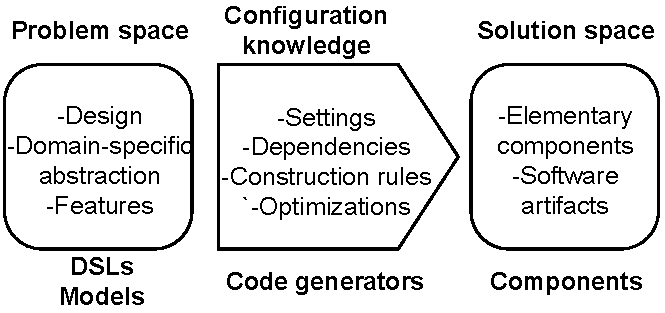
\includegraphics[scale=0.65]{Background/fig/GDM.pdf}
	\caption{Generative programming concept}
	\label{fig:GDM}
\end{figure}
%GP advantages
This schema integrates several powerful concepts from model driven engineering, such as domain-specific languages, feature modeling, and code generators.

Some commonly benefits of such software engineering process are:
\begin{itemize}
\item It reduces the amount of re-engineering/maintenance caused by specification requirements.
\item It facilitates the reuse of components/parts of the system.
\item It increases the decomposition and modularization of the system.
\item It handles the heterogeneity of target software platforms by automatically generating code.
\end{itemize}

An example of generative programming application is the use of Software Product Lines (SPL)\cite{schaefer2012software}.
SPL-based software diversity is often coupled to generative programming techniques\cite{Czarnecki:2000:GPM:345203} that enable the automatic production of source code from variability models. This technique implies the use of automatic code generators to produce code that satisfies user requirements (SPL models).
This technique enables one to manage a set of related features in order to build diverse products in a specific domain. Thus, this solution is able to control software diversity by handling the diversity of requirements such as user requirements or environmental constraints or changes. 

%In the following section, we present a general overview of the complete software development tool chain and the main actors that are involved from design time to runtime.


\subsection{Overview of the generative software development process}
The generative software development process involves many different technologies. In this section, we describe in more details the different activities and stakeholders involved to automatically transform the high-level system specifications into executable programs and that from design time to runtime.

Figure~\ref{fig:background_overview2} gives an overview of this process, as we see in the context of this thesis. We distinguish four main tasks necessary for ensuring the automatic code generation: 

\begin{figure}[h]
	\center
	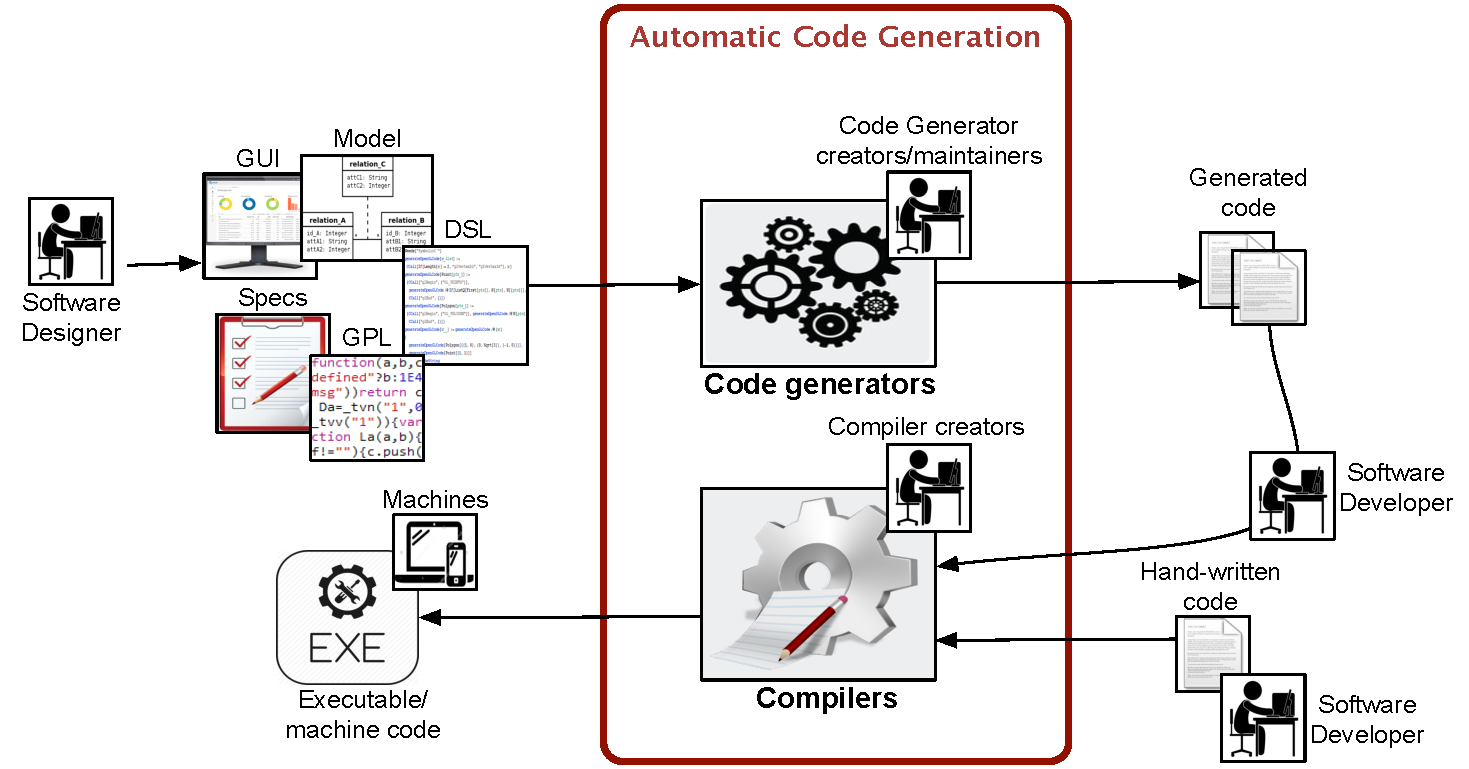
\includegraphics[scale=0.65]{Background/fig/background_overview2.pdf}
	\caption{Overview of the generative software development process}
	\label{fig:background_overview2}
\end{figure}
%\subsection{Automatic code generation}

\begin{enumerate}
	\item \textbf{\textit{Software design:}} 
	As part of the generative programming process, the first step consists on representing the system behavior. 
	%Software design/behavior is the input program for the code generators. 
	On the input side, we can either use code as the input or an abstract form that represents the design. It depends on the type of the code generator and on the input source program it requires. These programs can range from a formal specification of the system behavior to abstract models that represents the business logic.
	For example, designers can define, at design time, the software's behavior using for example Domain-Specific Models (DSMs).
	A DSM is a system of abstractions that describes selected aspects of a sphere of knowledge and real-world concepts pertinent to the domain that needs to be designed. These models are specified using high-level abstract languages (\ie, DSLs). %Domain-specific languages (DSLs) improve programmer productivity by providing high-level abstractions for the development of applications in a particular domain. Furthermore, software design can be provided as GUIs, GPLs, Models, etc.
	
	\item \textbf{\textit{Code generation:}} 
	Code generation is the technique of building code using programs. The common feature of the generator is to produce code that the software developer would otherwise write by hand.
	%There is no one style of code generation. 
	Code generators are generally seen as a black box which requires as input a program and generate as output a source code for a specific target software platform/language. %Generators can work on the command line or using a GUI. 
	Code generation can build code for one or more target language, once or multiple times. There are different varieties of code generation aspects and it highly depends on the input category as described in the previous step. 
	%Code generation techniques depends generally on these inputs.  
	For example, code generator developers use model-driven engineering techniques in order to automatically generate code. Instead of focusing their efforts on constructing code, they build models and, in particular, create model transformations that transform these models into new models or code. Thus, the code generation process starts by taking the previously defined specification in order to translate a model to an implementation in a target language. We will see in Section~\ref{bg:Types of code generators} the different types of code generators.
	
	
	%In general, there are two main categories of Automatic code generation: passive or active.  Passive code generators build the code once, then have nothing more to do with the code.  It is up to the discretion of the user as to how to update and maintain the code.  Active code generators, on the other hand, keep track of the code during its lifecycle.  Active code generators are run on code multiple times during the lifecycle.  With Active Code generators, there is code you can modify, and code that should only be modified by the code generator.  Code generators can be further classified into code mungers, inline code expanders, mixed code generators, partial class generators, tier generators and domain languages\cite{fertalj2008source}. 
	
	\item \textbf{\textit{Software development:}}
	Software development may be divided into two main parts. On the one hand, software developers may follow the two previous steps in order to automatically generate code for a specific target software platform. In this case, they might edit the system specification described in the first step (at a high level) and re-generate code each time needed by calling a specific generator. In some cases, generated code can even be edited by the end software developers. This task depends on the complexity of the generated code. Sometimes, it requires the help of domain experts who have enough expertise and knowledge to easily update and maintain the automatically generated code. On the other hand, they may manually implement the source code from scratch without going through any abstractions or code generation aspects. In this case, they may integrate the manually-written code with the automatically generated in order to deliver the final software product.
	
	\item \textbf{\textit{Compilation:}}
	Once code is generated or implemented, a classical compiler is used (if needed) to translate the generated code into an executable one. This translation depends on the target hardware platforms and it is up to the software developer to select the adequate compiler to use. Compilers are needed to target heterogeneous and diverse kinds of hardware architectures and devices. 
	As an example, cross compilers may be used to create executable code for a platform other than the one on which the compiler is running. In case the generated code needs to run on different machines/devices, the software developer needs to use different compilers for each target software platform and deploy the generated executables within different machines which is a tedious and time-consuming task.
	
\end{enumerate} 


\subsection{Automatic code generation in GP: a highly configurable process}
Among the main advantages that GP offers, is the automatic code generation, highlighted with red box in Figure~\ref{fig:background_overview2}. Automatic code generation emerges in two principal aspects: 
\begin{enumerate}
	\item The use of code generators to cope with software diversity and automatically generate code to a broad range of software platforms, as we discussed in Section \ref{sec:Software diversity}.
	\item The use of compilers to cope with hardware heterogeneity and automatically generate code to a broad range of hardware platforms, as we discussed in Section \ref{sec:Hardware diversity}.
\end{enumerate}

Both, compilers and code generators, are responsible for the automatic code generation in GP. To satisfy the different software and hardware requirements, modern generators provide many configuration options to easily tune the generated code: 

Compilers, on the one hand, become highly configurable and very user-friendly, letting the user to easily introduce optimizations and customize the machine code to fit with target hardware settings.
As an example, Table~\ref{iccgccllvm} depicts the number of optimizations available in three popular compilers. The user can configure the compiler by selecting one of the $2^{n}$ possible optimization sequences, where $n$ is the number of optimizations available in the compiler. We can see that the configuration space is very large. 

\begin{table}[h]
	\centering
	\caption{Number of optimizations in LLVM, GCC, and ICC}
	\label{my-label}
	\begin{tabular}{|c|c|c|}
		\hline
		\textbf{Compiler} & \textbf{\#Optimizations} & \textbf{\#Combinations} \\ \hline
		\textbf{LLVM}     & 100    & $2^{100}$                                 \\ \hline
		\textbf{GCC}      & 250    & $2^{250}$                                 \\ \hline
		\textbf{ICC}      & 75     & $2^{75}$                                 \\ \hline
	\end{tabular}
	\label{iccgccllvm}
\end{table}

On the other hand, code generators offer the possibility to customize the generated code for the target software platform. Code generators provide general configuration options necessary for building software artifacts (\eg, select the target programming language, dependencies, platform settings, libraries, etc.).
As an example, JHipster\footnote{https://jhipster.github.io/} is a concrete example of generative programming application in industry. JHipster is an application generator based on YO generator which provides tools to generate quickly modern web applications using Java stack on the server side (using Spring Boot) and a responsive Web front-end on the client side (with AngularJS and Bootstrap).
The generated web application can be quite different from one user to another. It really depends on the options/choices selected by the user to build a configured application. The selected parameter values will configure the way the JHipster code generators will produce code. 
For example, Figure~\ref{fig:jhipster} shows a feature model of some configuration examples that the user can select. When building applications, the user may select the database type he would generate, the Java version, the network protocol, etc. 
Using this feature model, \textbf{more than 10k diverse architecture types} of project can be selected which means that 10k program variants may be generated depending on the different criteria.
Whatever configuration selected by the user, the application behavior will not change and the generated application will share a similar architecture and fundamental code-base.
%Among the main contributions of this thesis, one is to evaluate the impact of applied configurations during code transformation/optimization (by whether code generators or compilers) on the resource usage requirements.
\begin{figure}[h]
	\center
	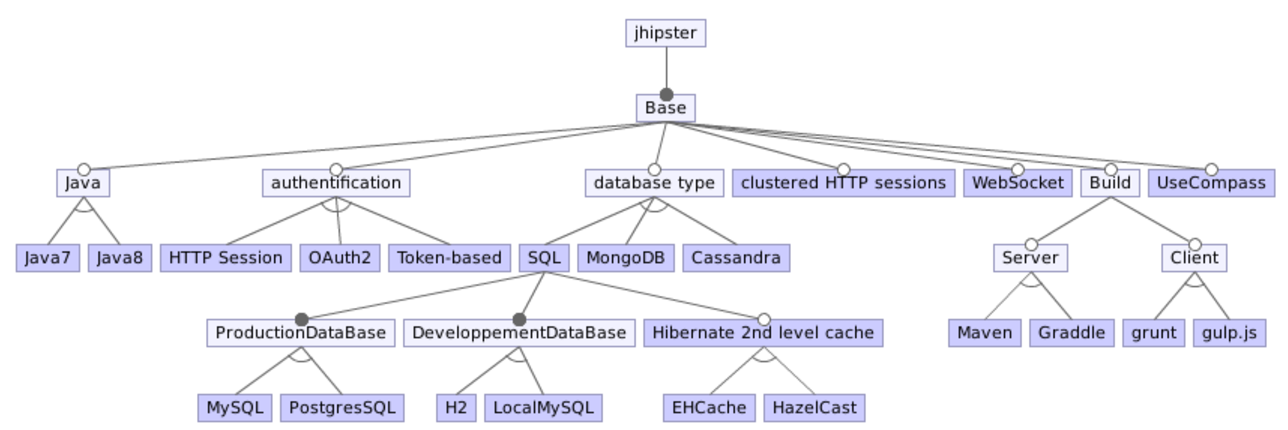
\includegraphics[scale=0.65]{Background/fig/jhipster}
	\caption{Example of JHipster feature model}
	\label{fig:jhipster}
\end{figure}

Well, we can see that both generators are highly configurable. However, in practice, code generators are less used in industry compared to compilers. First, because compilers are required for machine code production and optimization. Then, users of popular compilers such as GCC or LLVM have enough experience and confidence on the correct translation of the code. 
Code generators on the other side, are less used because users do not have enough experience with them and need to gain confidence on their correct operation by rigorously testing them. 
%The code generator user can gain confidence in the tool only if he run his own tests.

In summary, automatic code generation in GP faces two major challenges. On the one hand, configurable generators need to be efficiently tuned in order to produce high-quality software products. On the other hand, they have to be rigorously tested in order to provide evidence to the users of the efficiency of generated code.
%to trust and continue using them for production code generation.

We describe in the next section the main stakeholders involved in the automatic code generation in GP and their roles for validating this process.


\subsection{Stakeholders and their roles for testing and tuning generators}
\begin{figure}[h]
	\center
	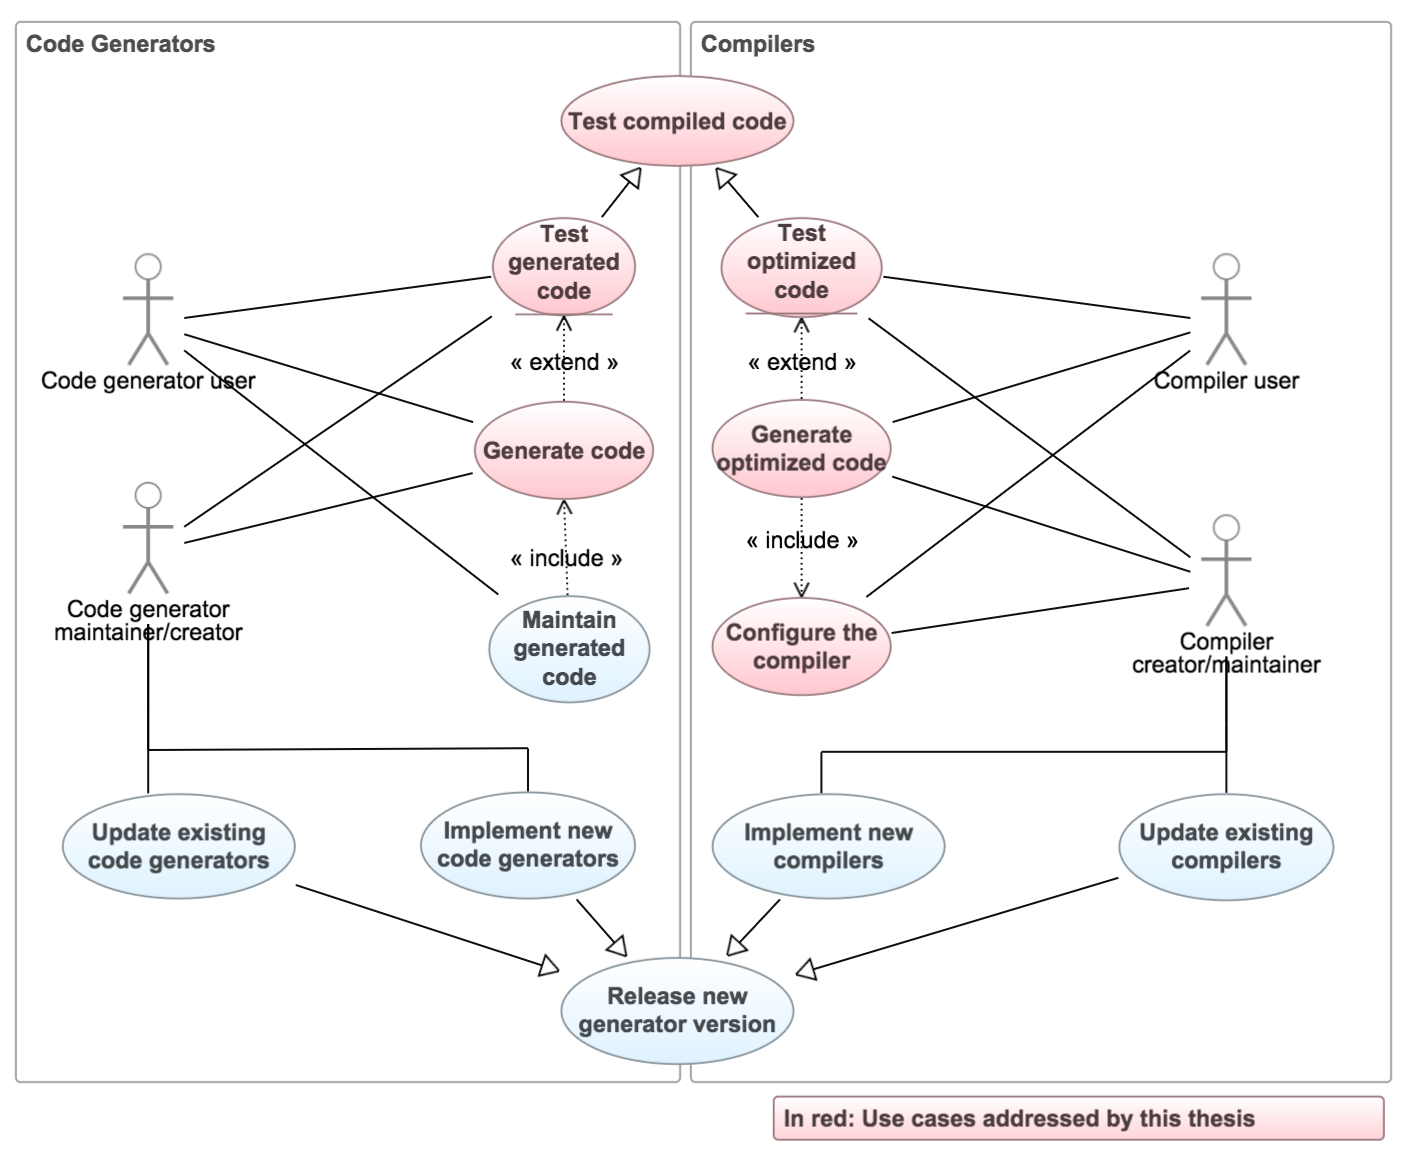
\includegraphics[scale=0.55]{Background/fig/usecase}
	\caption{Use case diagram of the different actors/roles involved in testing and tuning generators}
	\label{fig:usecase}
\end{figure}
Software development involves several stakeholders that play different roles for validating and testing the software development chain described previously.
Figure~\ref{fig:usecase} depicts a use case diagram that describes these different concerns, actors, and roles for testing and tuning generators.

Basically, we distinguish two stakeholders: generator users and creators/maintainers. As shown in the bottom of Figure~\ref{fig:usecase}, creators/maintainers are responsible of the correct functioning of generators. They use their expertise and knowledge associated to the software and hardware technologies, resulting in efficient code generation. They contribute to the software development community by creating and providing new generator updates (\eg, introduce new optimizations, build new platform-specific generators or enhance existing ones).

On the other side, generator users represent the group of software developers that have no knowledge/expertise about the way code is generated. Thus, they are unable to edit or maintain the internal behavior of generators (\eg, the case of commercial and off-the-shell generators). In this case, generators are used as black box components by engineers during software development to ease code production. Developers may configure generators in order to efficiently produce code for the target hardware platform (\eg, by providing a set of optimization options) or maintain/edit the generated code in case of automatic source code generation.

The use cases highlighted in red in Figure~\ref{fig:usecase} constitute the main tasks that we are addressing in this thesis. Our main concern is to evaluate the non-functional properties of automatically generated code. We involve two generator stakeholders, creators/maintainers and users (highlighted with red stereotypes). 
On the one hand, we would help code generator creator/maintainers to test the generated code and detect code generator issues by evaluating the resource usage and performance properties. This task may also involve code generator users but it is mainly the task of generator experts.
On the other hand, we would help compiler users to auto-tune compilers through the use of optimizations provided by compiler experts. It consists in evaluating the impact of these configurations on the performance and resource usage properties in order to find the best set of optimizations for a specific program and target hardware architecture.

%\begin{figure}[h]
%\center
%	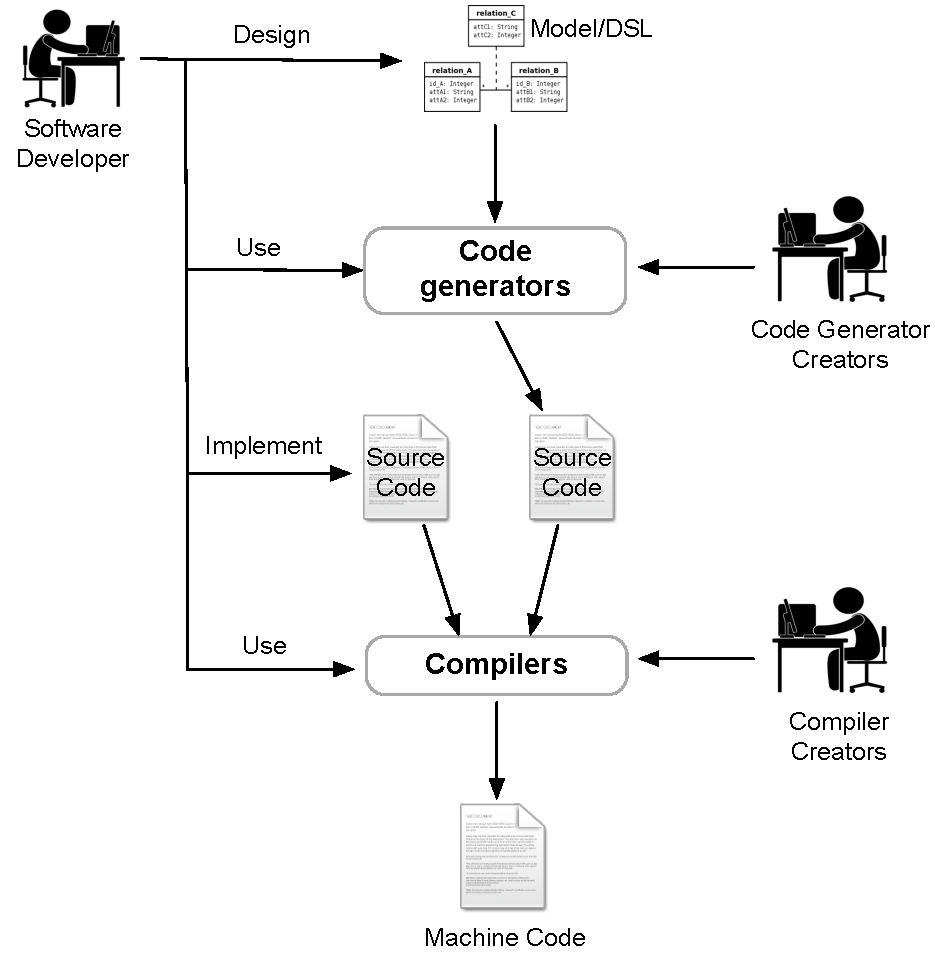
\includegraphics[scale=0.65]{Background/fig/background_overview.pdf}
%	\caption{Overview of the Docker-based testing architecture}
%\end{figure}

\section{Testing code generators}
\label{bg:Testing code generators}
In this thesis, we focus on testing the automatic code generation process (highlighted in red in the left side of Figure~\ref{fig:usecase}). To do so, we introduce in this section some basis about code generators. We give an overview of the different types of code generators and we discuss their complexity which constitutes a major obstacle for testing.
\subsection{Testing workflow}
The main goal of generators is to produce software systems from higher-level specifications.
\begin{figure}[h]
	\center
	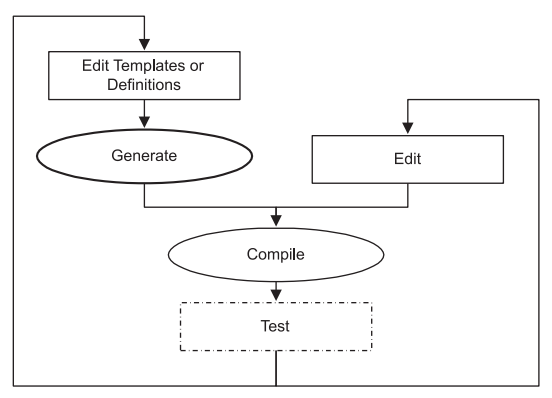
\includegraphics[scale=0.6]{Background/fig/workflow}
	\caption{Code generation workflow}
	\label{fig:workflow}
\end{figure}
As stated before, the code generation workflow is divided into two levels. It starts by transforming the system design into source code through the use of code generators. Afterwards, source code is transformed into executables using compilers. Thus, software developers use to generate code, edit it (if needed), compile it and then test it. If changes are applied to compilers or generators, the cycle is repeated. Figure~\ref{fig:workflow} presents an overview of this testing cycle. The right-hand side of the figure shows the classic workflow for developing and debugging code which is \textit{“edit, compile, and test”}. The user writes or edits an existing code, compiles it using specific compilers, and tests it. Code generation adds a few new workflow elements in the left-hand side of the figure where generator creators edit the templates and transformation rules (or the generator itself) and then run the code generator to create new output files. The output files are then compiled and the application is tested. 



\subsection{Types of code generators}
\label{bg:Types of code generators}
There are many ways to categorize generators. We can differentiate them by their complexity, by usage, or by their input/output. According to\cite{herrington2003code}, there are two main categories of automatic code generation: passive or active. Passive code generators build the code only once, then it is up to the user to update and maintain the code. 
The most common use of passive code generators are wizards. 

Active code generators, run on code multiple times during the lifecycle. With active code generators, there is code that can be edited by the users, and code that should only be modified by the code generator. Active code generators are widely referenced in the literature\cite{pais2005tool,amanquah2009rapid}. We focus in this thesis, on testing this class of code generators.
In the literature~\cite{herrington2003code,hunt2000pragmatic,fertalj2008source,bajovs2013code}, researchers define six categories of active code generators: 

\begin{itemize}
\item \textbf{Code munger:} A code munger reads code as input and then builds new code as output. This new code can either be partial or complete depending on the design of the generator.
A code munger is the most common form of code generators and are used widely. This kind of generators are often used for automatically generating documentations.
A source-to-source compiler, transcompiler or transpiler\footnote{\url{https://en.wikipedia.org/wiki/Source-to-source_compiler}} can also be defined as code mungers. A transcompiler takes a code written in some programming language and translates it to a code written in some other language. \textbf{Our contribution related to code generators testing will focus on this kind of generators to validate our approach for automatically detecting inconsistencies.}

Examples:  C2J, JavaDoc, Jazillian, Closure Compiler, Coccinelle, CoffeeScript, Dart, Haxe, TypeScript, and Emscripten



\item \textbf{Inline code expander:} This model reads code as input and builds new file that uses the input code as a base but with sections of the code expanded, based on the design of the original one. 
It starts with designing a new language. Usually this new language is an existing language with some syntax extensions. The inline code expander is then used to turn this language into production code in a high-level language.

Example: Embedded SQL languages such as SQLJ (for Java) and Pro*C (for C). The SQL can be embedded in the C or Java code. The generator builds production C code by expanding the SQL into C code which implements the queries for example.

\item \textbf{Mixed code generator:} This model has the same processing flow as the inline code expander, except that the input file is a real source file that can be compiled and ran. The generated output file keeps the original markup that will denote where the generated code is placed. It enables code generation for multiple small code fragments within a single file or distributed throughout multiple files. Generally, transformation rules are defined using regular expressions.


Example: Codify is a commercial mixed-code generator which can generate multiple code fragments in a single file from special commands. Another example is the replacement of comments in the input file by the corresponding code.

\item \textbf{Partial class generator:} A partial class generator takes an abstract definition as input instead of code (\eg, UML class diagram) and then builds the output code. User then, can extend it by creating derived classes and adding methods to complete the design. Turning models into code is done through a sequence of transformations. For example, platform-independent model (PIM) is transformed into a platform specific model (PSM). Then code generation is performed from PSM by using some sort of template-based code transformations.
%As an example, in model-driven engineering, a platform-dependent model (PIM) is transformed into a platform specific model (PSM). PIM to PSM translations are done either by hand or by applying automatic model transformation tools. Then code generation is performed from PSM by using some sort of template-based code generator.

Example: ArgoUML and Codegen translate UML class diagrams to general-purpose languages such as C\#, Java and C++. They do not generate complete implementations, but they try to convert the input UML class diagrams into skeleton code that the user can easily edit it. 

\item \textbf{Tier generator:} In this model the generator builds a complete set of output code from an abstract definition. It has the same concept as partial class generator. The big difference between tier and partial class generation is that in the tier model the generator builds all the code for a tier. This code is meant to be used without extension. The partial class generator model however, lets the engineer create the rest of the derived classes that will complete the functionality for the tier.
.
Examples: Database access layer, web client layer, data export, import, or conversion layers

\item \textbf{Full-domain language:} Domain languages are basically new languages that have types, syntax and operations and they are used for a specific type of problem. 
Domain languages are the extreme end of automatic code generation because developers have to write a compiler for each problem domain and language. 

Example: Matlab is a domain specific math language that makes it easy to represent mathematical operations. DSLs such as ThingML\footnote{\url{http://thingml.org/}} and its code generators.

\end{itemize}
%Generators are based on domain-specific models which define the semantics of the system specification language and also contain the knowledge of how to produce efficient implementations[REF]. 
%We distinguish two major types of code generators: rule-based model-to-model transformation languages (such as ATL) and template-based model-to-text transformation languages (such as Acceleo) to translate high-level system specifications into executable code and scripts.
\subsection{Why testing code generators is complex?}
\label{sec:Why testing code generators is complex?}
Testing code generators raise different challenges. In the following, we discuss some of them:
\begin{itemize}
	\item[--] \textbf{The oracle problem}: 
	
	To test the automatic code generation, test oracles are required to assess whether a test has passed or not. A test
	oracle checks whether the result of executing a test is as expected.
	In case of functional testing of code generators, the test oracle can be easily defined. For example, it can be defined as the comparison result between the simulated or executed model and its corresponding implementation. 
	However, in case of non-functional testing of code generators, the test oracle is complex to define. In fact, the generated code has to meet certain performance requirements (\eg, execution speed, utilization of resources, etc.). Proving that the generated code respects one of these non-functional requirements is not obvious. 
	%For example, one kind of solutions that can be applied is to perform a non-regression testing approach to compare the non-functional properties of two implementation versions of generated code.
	
	\item[--] \textbf{Infeasibility of unit testing}:
	 
	It is infeasible to test a whole code generator exhaustively with traditional software test approaches due to the complexity of the tool. When it comes to the unit testing of code generators, each translation function would have to be detached from the software system and surrounded by a test harness. This means decoupling each translation rule and testing it separately. This is, however, infeasible because it is difficult to address this specific functionality separately when testing a system as a whole. 
	Consider, for example, functional testing of the translation function for the sum operator (+). According to\cite{burnard2004verifying}, there are more than \num{2000} ways of implementing the function a = b + c since the operation depends on data types and whether data limiting is enabled or not.
		
	\item[--] \textbf{Complexity of code generators}: 
	
	Code generators can be difficult to understand since they are typically composed of numerous elements, whose complex interdependencies pose important challenges for developers performing design, implementation, and maintenance tasks. 
	Given the complexity and heterogeneity of the technologies involved in a code generator, developers who are trying to inspect and understand the code generation process have to deal with numerous different artifacts. As an example, in a code generator maintenance scenario, a developer might need to find all chained model-to-model and model-to-text transformation bindings, that originate a buggy line of code to fix it. This task is error prone when done manually\cite{guana2015developers}. 
%	So, flexible traceability tools are needed to collect and visualize information about the architecture and operational mechanics of code generators, to reduce the challenges that developers face during their life-cycle\cite{guana2015developers}. 
		\begin{table}[h]
			\centering
			\sisetup{table-number-alignment = right}
			\caption{Metrics of the TargetLink code generator}
			\begin{tabular}{| l | S | }\hline
				\textbf{Metrics} & \textbf{TargetLink code generator 2.0}  \\	\hhline{|=|=|}	
				No. of classes  & 3000\\ 
				No. of files & 6000 \\  
				No. of functions & 51000 \\  
				Lines (total) & 1800000 \\  
				Lines of code & 990000 \\ 
				Lines of comments  & 560000 \\ 	\hline
			\end{tabular}
			\label{tab:targetlinkk}
		\end{table}
	Table~\ref{tab:targetlinkk} shows, as an example, some metrics of the TargetLink code generator version 2.0. TargetLink\footnote{\url{https://www.dspace.com/en/inc/home/products/sw/pcgs/targetli.cfm}} is a code generator that generates production code (C code) straight from the MATLAB/Simulink/Stateflow graphical models. 
	This table shows how huge is the code generator base code. With more than \num{1800000} lines of code, it is very hard to test the whole system. 
	
	\item[--] \textbf{Non-executable source model}: 
	
	Code generators do not always support executable source models. Sometimes, code generators such as partial class generator, generate only structural code through a series of transformations from a non-executable model (\eg, UML diagrams). It is up to the users next, to extend the generated code by implementing the derived classes. 
	In case of non-executable models, it becomes challenging to automatically verify the correct behavior of produced code as it is described in the model specification because we can not compare its execution to a simulated model for example.
	   

	
	%The challenge is that the structure of the specification is usually very different from the structure of the implementation: there is no simple one-to-one correspondence between the concepts in the specification and the concepts in the implementation. 
\end{itemize}

%Efficient implementations are then computed at generation time by applying domain-specific optimizations and replacing, merging, adding, and removing components.

%\begin{figure}[h]
%	\center
%	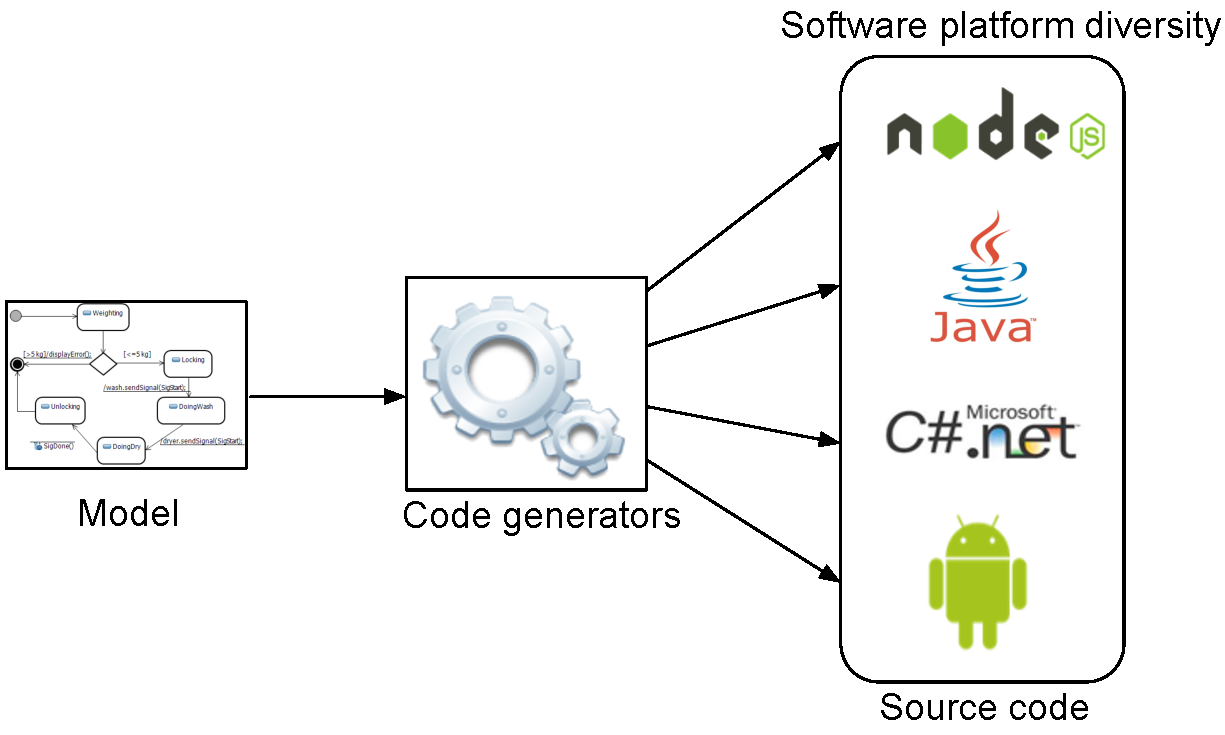
\includegraphics[scale=0.65]{Background/fig/software-diversity.pdf}
%	\caption{Code generation process}
%\end{figure}




\section{Compilers auto-tuning}
\label{bg:Compilers auto-tuning}
%The compiler is a very essential software component in software engineering, responsible for translating user's source code written in general purpose languages into machine code. The key feature of compilers is to bridge source programs written in high-level languages with the underlying hardware architecture. High-level languages are used to help the software developer to have an easier and simpler way for writing programs. They offer many abstract programming features such as functions, data structures, conditional statements and loops that facilitate the software development. During software development, developers intend to write understandable and maintainable code without putting too much emphasizes on the performance for example. This means that the 

Compilers have a major role in automatically producing fast and efficient target machine code. This is not a trivial task because potentially many variants of the machine code exist for the same program. Hence, the task of the compiler is to find and produce the best version of the machine code for any given program. For this reason, compilers generally attempt to automatically optimize the code to improve its performance.
This process is called code optimization. 

\subsection{Code optimization}

Code optimization within a compiler is the process of transforming a source code program into another functionally equivalent code for the purpose of improving one or more of its non-functional properties. 
The most common outcome of optimizations is the performance improvement. Other less common non-functional properties are code size, memory usage and power consumption. 
There exist many types of optimizations such as loop unrolling, automatic parallelization, code-block reordering, and functions inlining, among others. The hardware characteristics that influence on the optimization's impact may include: the number of CPU registers (the more registers, the easier it is to optimize for performance), cache size, CPU architecture, etc.

Optimization can be categorized broadly into two types: machine independent and machine dependent: 
\begin{itemize}
	
	\item \textbf{Machine-independent optimization:}
	
	Intermediate code generation inside compilers may introduce many inefficiencies such as extra copies of variables and using variables instead of
	constants.
	This kind of optimization removes such inefficiencies and improves code. Thus, the compiler takes in the intermediate code and transforms a part of the code regardless of any CPU registers or memory locations. These optimizations generally change the structure of programs.
	Optimizations that are applied on abstract programming concepts (structures, loops, objects, functions) are independent of the machine targeted by the compiler.
	
	\textbf{Example:} Eliminate redundancy, loop unrolling, eliminate useless and unreachable code, function inlining, dead-code elimination, etc.
	
	\item \textbf{Machine-dependent optimization:} 
	Machine-dependent optimizations are applied after generating the target code and when the code is transformed according to the target machine architecture. They take advantage of special hardware features to produce code which is shorter or which executes more quickly on the machine such as instruction selection, register allocation, instruction scheduling, parallelism, etc.
	They mostly involve CPU registers and memory references. Machine-dependent optimizers put efforts to take maximum advantage of the memory hierarchy. They are more effective and have better impact on performance than independent optimizations because they best exploit special features of the target hardware.
	
	\textbf{Example:} Register allocation optimizations for efficient utilization of registers, branch prediction, loop optimization, etc.
 
 
\end{itemize}
 

 
 
 

\subsection{Why compilers auto-tuning is complex?}
\label{sec:Why compilers auto-tuning is complex?}
%\subsection{Why complier auto-tuning is complex?}
Today, modern compilers implement a broad number of optimizations. Each optimization tries to improve the performance of the input application.

On the one hand, optimizing compilers becomes quite sophisticated nowadays. Creating compiler optimizations for a new microprocessor is a hard and time-consuming work because it requires a comprehensive understanding of the underlying hardware architecture as well as an efficient way to evaluate the optimization impact on the non-functional properties. 

On the other hand and from the compiler user perspective, applying and evaluating optimizations is challenging because the determination of the optimal optimization set has been identified as a major research problem in the literature\cite{knijnenburg2002iterative}.

We resume, in the following, several issues that make the activity of compiler auto-tuning very complex:

\begin{itemize}
	\item[--] \textbf{Conflicting objectives:} Compilers optimizations have to support a variety of conflicting objectives, such as execution time/compilation speed, execution time/resource usage, etc. It is difficult to define a set of optimizations that satisfies all properties.
	
	\item[--] \textbf{Optimization interactions:} The interaction between optimization phases as well their application order make it difficult to find an optimal sequence.
	
	\item[--] \textbf{Huge number of optimizations:} The huge number of optimizations is also an issue for the compiler user to choose the best optimization sequence since an exhaustive search is impossible (we count $2^{number\ of\ optimizations}$ possible combination to evaluate).
	
	\item[--] \textbf{Non universal optimizations:} There is no universal optimization sequence that will enhance the performance of all programs. Optimization's impact depends on the hardware and on the input program. Thus, constructing an optimization sequence for different programs and hardware architectures becomes very hard.
	
	\item[--] \textbf{Compiler bugs:} Applying optimizations may introduce errors in the compiled code and results in compiler bugs\cite{le2014compiler,yang2011finding}. Therefore, tuning compiler must not cause any change in the program behavior.
	
	\item[--] \textbf{Optimization impact:} Optimized code should be fast and efficient. Optimizations have to improve some non-functional properties, not to induce performance regressions/overhead.
	
	\item[--] \textbf{Tuning compilers need expertise:} In case the compiler user has no knowledge and expertise about the compiler technology and its optimizations, it will be quite hard to select the set of optimization sequences to apply.
\end{itemize}

 

%Improvement of source code programs in terms of performance can refer to several different non-functional properties of the produced code such as code size, resource or energy consumption, execution time, among others~\cite{almagor2004finding,pan2006fast}.
%\begin{figure}[h]
%	\center
%	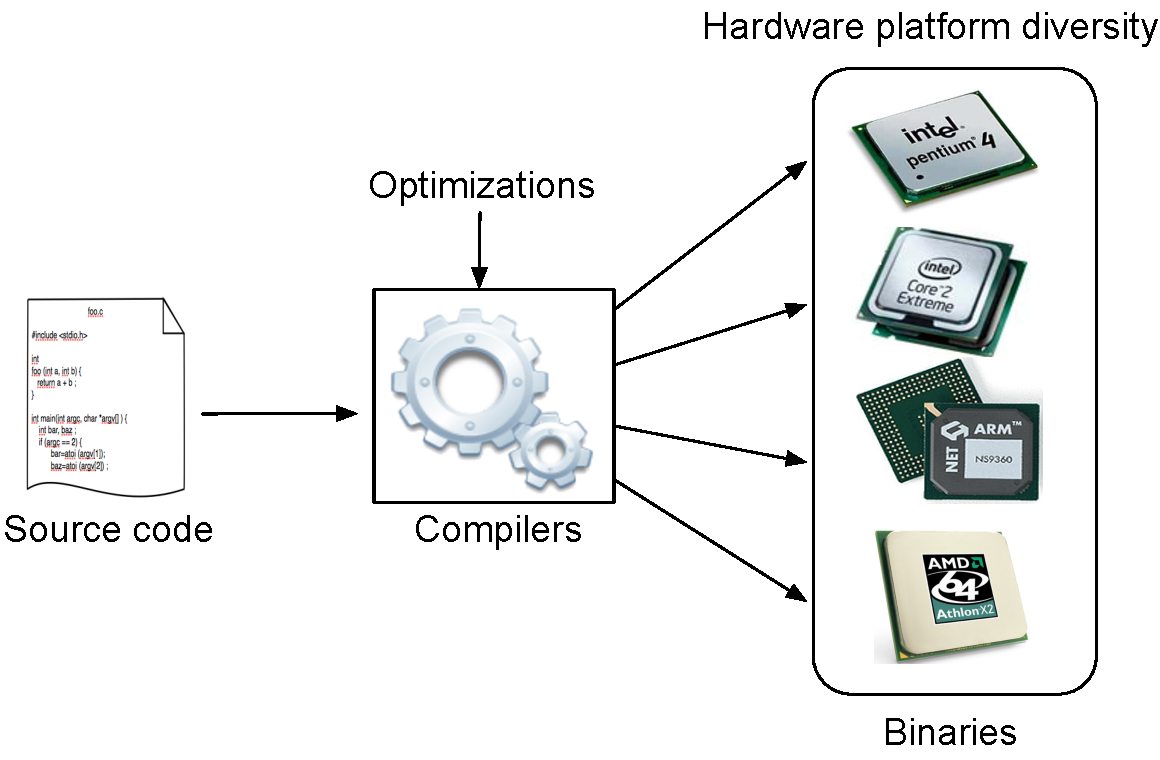
\includegraphics[scale=0.65]{Background/fig/hardware-diversity.pdf}
%	\caption{Compiler optimizations}
%\end{figure}


\section{Summary: challenges for testing and tuning configurable generators}
\label{bg:Summary: Testing and optimization challenges}
We resume in this section the main testing and tuning challenges we have identified throughout this chapter:
\begin{itemize}
	\item \textbf{Heterogeneous execution environments}: 
	The diversity of existing software environments and platforms as well as the hardware heterogeneity make the testing activity of generators very difficult. Deploying and executing the automatically generated software artifacts on top of a bench of platforms is time consuming. Thus, an effective mean is needed to facilitate generators testing and tuning.
	\textbf{How can we leverage the new advances in software engineering technologies to face the continuous hardware and software innovation when testing/tuning generators?} 
	
    \item \textbf{The oracle problem when testing code generators}: 	
	Automatic code generation offers many gains over traditional software development methods (\eg, speed of development, productivity, etc.). However, code generators are complex pieces of software that may themselves contain bugs. Thus, they need to be rigorously tested. The test oracle problem as discussed in Section~\ref{sec:Why testing code generators is complex?} is one of the main challenges related to the automatic non-functional testing of code generators. This problem occurs also in automatic functional testing, when dealing with non-executable models.
	\textbf{
	%So, how can we automatically detect issues within code generators? 
	Proving that the generated code is functionally correct is not enough to claim the effectiveness of the code generator under test? How about the non-functional requirements such as resource consumption?
	How can we efficiently detect the non-functional issues?}
	
	\item \textbf{Large optimization search space when auto-tuning compilers}: 
	Compilers may have a huge number of potential optimization combinations, making it hard and time-consuming for software developers to find/construct the sequence of optimizations that satisfies user specific key objectives and criteria. It also requires a comprehensive understanding of the available optimizations of the compiler and their interactions. Moreover, it is difficult to find the optimization sequence that represents a trade-off between two conflicting objectives.  
	\textbf{So, how can we help compiler users to automatically tune compilers and choose the optimization set that satisfies some specific non-functional requirements? }
	
	\item \textbf{Monitoring the resource usage of automatically generated code:} 
	Analyzing the resource usage of optimized or generated code requires a dynamic and adaptive solution that efficiently extracts those properties. Due to the software diversity and hardware heterogeneity, monitoring the resource usage of each execution platform becomes challenging and time-consuming. 	
	\textbf{So, how can we ease this process and provide efficient support to help generator users/experts to evaluate the non-functional behavior of generated code in terms of resource usage?}
	

	

%\subsection{Resource usage monitoring}
\end{itemize}


%

\chapter{State of the art}
In this chapter, we study existing techniques related to code generators testing as well as compilers auto-tuning techniques.
Section 3.1 provides a survey of the most used compiler auto-tuning techniques to construct the best set of optimization options. In Section 3.2, we review existing techniques for code generators testing. Section 3.3 discusses the limitations of the state of the art.
\section{Compilers auto-tuning techniques}

\subsection{Iterative compilation}
Iterative compilation or also known by optimization phase selection consists on applying software engineering techniques to produce better and more optimized programs by compiling multiple versions of each of them using different optimizations settings. After running these versions on specific hardware machines, the key objective of iterative compilation is to find the best optimizing sequence that lead to the fastest and better code machine code. 
Our work is related to iterative compilation research field.
The basic idea of iterative compilation is to explore the compiler optimization space by measuring the impact of optimizations on software performance.
Several research efforts have investigated this optimization problem using search-based techniques (SBSE) to guide the search towards relevant optimizations regrading performance, energy consumption, code size, compilation time, etc. Experimental results have been usually compared to standard compiler optimization levels.  

It has been proven that optimizations are highly dependent on target platform and input program. 
Compared to our proposal, none of the previous work has studied the impact of compiler optimizations on resource usage. In this work, we rather focus on compiler optimizations related to resource consumption, while bearing in mind the performance improvement.

\subsection{Implementation of iterative compilation system}
\begin{figure}[h]
	\center
	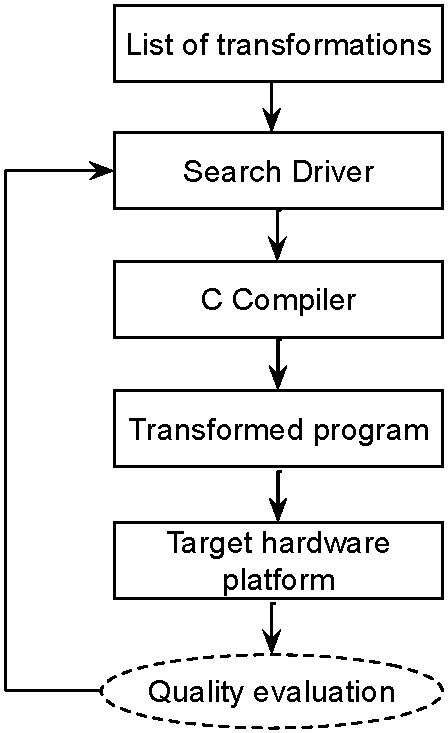
\includegraphics[scale=0.65]{SOTA/fig/iterative_compilation}
	\caption{Overview of the iterative compilation process}
	\label{fig:iterative_compilation}
\end{figure}
The implementation of iterative compilation consists mainly on applying a series of steps to enhance the quality of generated code. Figure~\ref{fig:iterative_compilation} shows a general overview of the principal steps needed to ensure the implementation of the iterative compilation process.
\begin{itemize}
	\item[--] List of transformations:
	The iterative process starts by defining the optimizations space. It represents the list of optimizations that the compiler have to apply during the search to enhance the software quality.
	\item[--] Search driver:
	It applies a search algorithm or method to efficiently explore the large optimization search space. In fact, it reads the previously defined list of transformations that it needs to examine and decides which transformations have to be applied next using a search algorithm
	to steer through the optimization space.
	\item[--] C Compiler:
	Once the optimization sequence is defined, the target C compiler for example is called to compile the input program and also perform initial machine independent optimizations. 
	\item[--] Transformed program:
	This results in initial machine independent optimized program. These optimizations are performed during code generation and have consequence for all target systems. It includes optimizations that are applied during mapping the parse tree to intermediate code and optimization applied to the intermediate code itself.
	\item[--] Target hardware platform:
	To optimize even more, the compiler applies from the provided optimization sequence the machine dependent optimizations. They are specific to the object code being generated. This includes optimizations applied during the mapping of intermediate code to assembler and optimizations applied directly on the generated
	object code.
	\item[--] Quality evaluation:
	It consists on evaluation the quality of the optimized code. Many non-functional properties could be evaluated like code size, execution time, resource usage, power consumption, etc...
	
\end{itemize}

This model represents the classical and typical iterative compilation process. Of course, there exist many ways and adaptations to implement this process. The implementation of the iterative process depends on the algorithm used, the problem addressed, the technologies used, etc. The goal of the next section is to present the different state-of-the-art approaches related to iterative compilation.

\subsection{Iterative compilation search techniques}
In section 2.5.2 of chapter 2, we presented several issues with optimizing compilers that make the activity of compiler tuning very complex such as the huge number of optimizations, conflicting objectives, optimization overhead, etc.
In this section, we discuss the available tools and approaches dedicated to the automatic search for optimal compiler settings, and give an overview of known approaches that addressed the several compiler optimization challenges. In each subsection, we identify and discuss a particular problem and we present the best known approaches proposed to solve it.

\subsubsection{Speeding up the performance: a mono objective optimization}
Speeding up the performance of compiled code is the key optimization objective for most of the iterative compilation approaches. The problem has been often adapted as a mono-objective optimization problem where the speedup has been the main concern. Genetic algorithms (GA)\cite{stephenson2003genetic,bashkansky2007black} present an attractive solution to this problem of selecting an optimal set of options. 
GA-based approaches compute an initial population using a set of optimizations, generally defined under the standard compiler levels Ox. Then, at each iteration, the individuals (i.e., option sets) that comprise the generation are evaluated by measuring for example the execution time resulted by a specific set of options. The results are sorted and pass through a breeding and mutation stage to form the next generation. This
process continues until a termination condition is reached. The algorithm return the best optimization set that led to the highest performance.

The ESTO framework described in \cite{bashkansky2007black} studies the application of GA for the problem of selecting an optimal option set for a specific application and workload. It searches the option set space using various types of genetic algorithms, ultimately determining the option set that maximizes the performance of the given application and workload. ESTO regards the compiler as a black box, specified by its external-visible optimization options. The algorithm used in ESTO is the GA. It supports also a GA variant named budget-limited genetic algorithm which reduces the population size exponentially and then reduce the time needed to evaluate the different evaluations. They ran experiments on the SPEC2000 benchmark suite and tested 60 optimization options within three compilers: GCC, XLC and FDPR-Pro. Results of ESTO are compared to GCC -O1 and -O3, to XLC -O3 and to FDPR-Pro -O3. The results show that ESTO is capable to construct optimization levels that yield to better performance than standard options.



\subsubsection{JIT compiler optimization}
\subsubsection{Escaping local optimum}
\subsubsection{Dealing with numerical parameter values}
This problem is related to numerical parameters optimization where the parameter optimization value should be determined automatically
\subsubsection{Evaluating iterative optimization across multiple data sets}
Most iterative optimization studies find the best compiler optimizations through repeated runs on input program and the same data set. The problem is that if we select the best optimization sequence for an input data set through the iterative process, we do not know if it will still be the best for the same program but with other data sets. Thereby, researchers in this field try to investigate this problem by evaluating the effectiveness of iterative optimization across a large number of data sets. In particular, since there is no existing benchmark suite with a large number of data sets  Chen et al.\cite{chen2010evaluating} attempt to collect 1000 data sets called KDataSets for 32 programs, mostly derived from the MiBench benchmark. Then, they exercise iterative optimization on these collceted data sets in order to fin the best optimization combination across all data sets. 
They used random search to generate random optimization sequences for the ICC compiler (53 flags) and the GCC compiler (132 optimizations).
They demonstrate that for all 32 programs (from MiBench), they were able to find at least one combination of compiler optimizations that achieves 86\% or more of the best possible speedup across all data sets using Intel’s ICC (83\% for GNU’s GCC). This optimal combination is program-specific and yields speedups up to 1.71 on ICC and 2.23 on GCC over the highest optimization level (-fast and -O3, respectively). This means that a program can be optimized on a collection of data sets and it can retain near optimal performance for most other data sets. So the problem of finding the best optimization for a particular program may be significantly less complex. However, they tested their approach on only one single benchmark and one target architecture.
\subsubsection{Phase ordering problem}
Phase ordering is also an important problem in iterative compilation which explores the effect of different orderings of optimization phases on program performance. In fact, using some compilers such as LLVM, it is important to define the right order of applying optimizations. Thus, researchers in this field try to apply search techniques in order to find the right optimization sequence. However, reordering optimization phases is extremely hard to support in most production systems, including GCC due to their use of multiple intermediate formats and complex inherent dependencies between optimizations. So generally, compilers manage internally the order of applying optimizations and do not give the hand to the user to choose this order to avoid conflicts and compilation issues.


\subsubsection{Conflicting objectives: a multi-objective optimization}
The vast majority of the work on iterative compilation focuses on increasing the speedup of new optimized code compared to standard compiler optimization levels. However, they do not put too much emphasis on finding trade-offs between two (or more) non-functional properties ~\cite{almagor2004finding,hoste2008cole,pan2006fast,pallister2015identifying,chen2012deconstructing,martins2014exploration,lin2008automatic,martinez2014multi}.

In COLE\cite{hoste2008cole}, the authors considered that the problem of compiler optimizations can be seen as a multi-objective problem where two non-functional properties can be enhanced simultaneously. Thus, they investigated the standard levels of compiler optimization by searching for Pareto optimal levels that maximize both performance and compile time. 
They show that by using the multi-objective genetic algorithm (in their experiment they used SPEA2), it’s possible to find a set of compiler optimization sequences that are more Pareto-effective in terms of performance and compile time than the standard optimization levels (-O1, -O2, -O3, and -Os). The motivation behind this approach is that these standard level were set up manually by compiler creators based on fixed benchmarks and data sets. For authors, these universal levels may not be always effective on unseen programs and there exist higher levels that provide better trade offs in terms of code quality.
The authors used SPEC2000 CPU benchmark, which is a popular benchmark suite for evaluating the compiler performance. They evolved 60 optimization flags that are defined in the standard levels O1, O2, O3, O1 and OS. They run iterative compilation on one single machine shipped with Intel CPU Pentium 4 and they compared the proposed algorithm (SPEA2) to random search as well as to standard optimization levels.

The experimental results using GCC (v4.1.2) show that the automatic construction
of optimization levels is feasible in practice, and in addition, yields better optimization levels than GCC’s manually derived (-Os, -O1, -O2 and -O3) optimization levels, as well as the optimization levels obtained through random sampling.
However, They do not provide a guarantee that the new explored optimization levels selected for SPEC still will be optimal for other applications.


In another story, Martinez et al.\cite{martinez2014multi} propose an adaptive worst-case execution time WCET-aware compiler framework for automatic search of compiler optimization sequences which yield highly optimized code. 
Compared to previously described approach authors in this paper focus on generating efficient code for embedded systems. Embedded systems are characterized by both efficiency requirements and critical timing constraints. Properties as Average-case performance, power consumption and resource utilization are the main concerns describing the efficiency of a system. 
Thus, they explore the performance of compiler optimizations with conflicting goals. 
Besides the objective functions average-case execution time and code size, they consider the WCET which is a crucial parameter for real-time systems, especially for
safety-critical application domains such as automotive and
avionics to avoid system failure. 
Then, they try to find suitable trade-offs between these objectives in order to identify Pareto optimal solutions using stochastic evolutionary multi-objective algorithms. The objective functions try to minimize the WCET-ACET and WCET-Code size properties. They apply three evolutionary multi-objective algorithms (EMO) namely IBEA, NSGA-II and SPEA2 and compared their results to standard levels (O1, O2 and O3). 
They evolved 30 optimizations within the WCC compiler and performed experiments on top of one single machine shipped with Intel Quad-Core CPU processor. They pick up as well 35  programs from various benchmarks such as DSPstone, MediaBench, MiBench, etc.
They found that NSGA-II is the most promising EMO for the given problem. In fact, the discovered optimization sequences significantly outperform standard optimization levels:
the highest standard optimization level O3 can be outperformed for the WCET and ACET on average by up to 31.33\% and 27.43\%, respectively. The same approach performs as well for the WCET-Code size optimization with a 30.6\% WCET reduction over O3. However, the code size increases by 133.4\%. This is because the WCET and the code size are typical conflicting goals. If a high improvement of one objective function is desired, a significant degradation of the other objective must be accepted.

\subsubsection{Predicting optimizations: a machine learning optimization}
Machine learning has been also proposed by several works to tune optimizations across programs. Compared to evolutionary algorithms, using machine learning in compiler optimization has the potential of reusing knowledge across the different iterative compilation runs, gaining the benefits of iterative compilation to learn the best optimizations across multiple programs and architectures.
In the Milepost project\cite{fursin2011milepost} for example, authors start from the observation that similar programs may exhibit similar behavior and require similar optimizations so it is possible to correlate program features and optimizations together to predict good transformations for unseen programs based on previous optimization experience. Thereby, they provide a modular, extensible, self-tuning optimization infrastructure that can automatically learn how to best optimize programs for configurable heterogeneous processors based on the correlation between program features, run-time behavior and optimizations. 

The proposed infrastructure is based on a machine learning compiler that present an Interactive Compilation Interface (ICI) and plugins to extract program features (such as the number of instructions in a method, number of branches, etc) and select optimization passes. 

The Milepost framework currently proceeds in two distinct phases: training and deployment. During the training phase, information about the structure of programs (input training programs) is gathered, showing how they behave under different optimization settings. Such information allows machine learning tools to correlate aspects of program structure, or features, with optimizations, building a strategy that predicts good combinations of optimizations. 
After running an iterative process that evaluates different combinations of optimizations on top of the training programs/features, pedictive models are created to correlate a given set of program features with profitable program transformations. 
Then, in the deployment phase, the framework analyzes new unseen programs by determining the program’s features and passes them to the new created models to predict the most profitable optimizations to improve execution time or other metrics depending on the user’s optimization requirements.

GCC was selected as the compiler infrastructure for Milepost as it is currently the most stable and robust open-source compiler. They evolved 100 optimization flags under O1, O2 and O3 levels and compared their results to the O3 level and to the random search.

The experimental results show that it is possible to improve the performance of the MiBench benchmark suite automatically using iterative compilation and machine learning on several platforms including x86: Intel and AMD, and the ARC configurable core family. Using the machine learning-based framework , they were also able to learn a model that automatically improves the execution time of some individual MiBench programs by a factor of more than 2 while improving the overall MiBench suite by 11\% on reconfigurable ARC architecture, without sacrificing code size or compilation time. Furthermore, their approach supports general multi-objective optimization where a user can choose to minimize not only execution time but also code size and compilation time.




 

\iffalse
Novelty Search has never been applied in the field of iterative compilation. Our work presents the first attempt to introduce diversity in the compiler optimization problem. 
The idea of NS has been introduced by Lehman et al.~\cite{lehman2008exploiting}. It has been often evaluated in deceptive tasks and especially applied to evolutionary robotics~\cite{risi2010evolving,krvcah2012solving} (in the context of neuroevolution). 
NS can be easily adapted to different research fields. In a previous work~\cite{boussaa2015novelty}, we have adapted the general idea of NS to the test data generation problem where novelty score was calculated as the Manhattan distance between the different vectors representing the test data. The evaluation metric of generated test suites is the structural coverage of code.
In this paper, the evaluation metric represents the non-functional improvements and we are calculating the novelty score as the symmetric difference between optimization sequences. 

For multi-objective optimizations, we are not the first to address this problem. New approaches have emerged recently to find trade-offs between non-functional properties~\cite{hoste2008cole,martinez2014multi,lokuciejewski2010multi}. Hoste et al.~\cite{hoste2008cole}, which is the most related work to our proposal, propose COLE, an automated tool for optimization generation using a multi-objective approach namely SPEA2. In their work, they try to find Pareto optimal optimization levels that present a trade-off between execution and compilation time of generated code. Their experimental results show that the obtained optimization sequences perform better than standard GCC optimization levels. NOTICE provides also a fully automated approach to extract non-functional properties. However, NOTICE differs from COLE because first, our proposed container-based infrastructure is more generic and can be adapted to other case studies (i.e., compilers, code generators, etc.). Second, we provide facilities to compiler users to extract resource usage metrics using our monitoring components. Finally, our empirical study investigates different trade-offs compared to previous work in iterative compilation.
\fi





%For code generators testing, Stuermer et al.~\cite{stuermer2007systematic} present a systematic test approach for model-based code generators. They investigate the impact of optimization rules for model-based code generation by comparing the output of the code execution with the output of the model execution. 
%If these outputs are equivalent, it is assumed that the code generator works as expected. 
%They evaluate the effectiveness of this approach by means of testing optimizations performed by the TargetLink code generator. 
%They have used Simulink as a simulation environment of models. 
%In our approach, we provide a component-based infrastructure to compare non-functional properties of generated code rather than functional ones. 


\section{Testing code generators}
Previous work on non-functional testing of code generators focuses on comparing, as oracle, the non-functional properties of hand-written code to automatically generated code~\cite{stepasyuk2015evaluating,richard2013efficient}. As an example, Strekelj et al.~\cite{vstrekelj2015performance} implemented a simple 2D game in both the Haxe programming language and the native environment and evaluated the difference in performance between the two versions of code. They showed that the generated code through Haxe has better performance than hand-written code. 

Cross-platform mobile development has been also part of the non-functional testing goals since many code generators are increasingly used in industry for automatic cross-platform development. In \cite{pazirandeh2015evaluation,hartmann2011cross}, authors compare the performance of a set of cross-platform code generators and presented the most efficient tools.

The container-based infrastructure has been also applied to the software testing, especially in the cloud~\cite{li2015rest}. Sun et al.~\cite{sun2016roar} present a tool to test, optimize, and automate cloud resource allocation decisions to meet QoS goals for web applications. Their infrastructure relies on Docker to gather informations about the resource usage of deployed web servers. 

Most of the previous work on code generators testing focuses on checking the correct functional behavior of generated code. Stuermer et al.~\cite{stuermer2007systematic} present a systematic test approach for model-based code generators. They investigate the impact of optimization rules for model-based code generation by comparing the output of the code execution with the output of the model execution. 
If these outputs are equivalent, it is assumed that the code generator works as expected. 
They evaluate the effectiveness of this approach by means of testing optimizations performed by the TargetLink code generator. 
They have used Simulink as a simulation environment of models. 
In \cite{jorges2014back}, authors presented a testing approach of the Genesys code generator framework which tests the translation performed by a code generator from a semantic perspective rather than just checking for syntactic correctness of the generation result.

Compared to our proposal, none of the previous work has provided an automatic approach for testing and monitoring the generated code in terms of non-functional properties. 

\subsection{Metamorphic testing techniques}
Most of the work on software testing seeks to automate as much as possible the testing process to make it faster, cheaper, and more reliable. 

To this end, automatic program testing involves in selecting suitable inputs as test cases, executing the program and verifying results against expected results. 
The mechanism against which the software tester verify whether the outputs of the program for the executed test cases are correct or not is called test oracle. 

For instance, the problem of automatically generating test inputs/data has been the subject of research interest for a long time. It consists on automatically generating test data and test cases that reveal faults/crashes or that maximize the code coverage of the system under test finding inputs that cause execution. Many techniques especially search-based testing techniques have been proposed to solve and automate this process\cite{ali2010systematic}.

However, compared to many aspects of test automation, the problem of automating the test oracle is still challenging and less well solved. This is because the test oracles are not always available and may be hard to define or too difficult to apply\cite{barr2015oracle}. This is commonly known as the “oracle problem”.

A metamorphic testing (MT) method has been proposed to alleviate the oracle problem\cite{chen2004case}. MT is an automated testing method that employs expected properties of the target functions to test programs without human implication. 
MT recommends that, given one or more test cases (called source or original test cases) and their expected outcomes, one or more follow-up test cases can be constructed to verify the necessary properties (called Metamorphic Relations MRs) of the system or function to be implemented.
For a given problem, usually more than one MR can be identified. It is therefore interesting to select effective MRs that are good at detecting program bugs.



\section{Container-based testing techniques}

Using virtual machines (VMs) as a mechanism for deploying and testing applications in the cloud is very useful to run application workload in heterogeneous and distributed environments.
In industry, a number of commercial usage scenarios benefit from virtualization techniques to provide services to the end users. For example, Amazon EC2 makes VMs available to the customers who can use them to run their own computer applications or services. Thus, a user can create, launch and terminate new VMs as needed.  

However, VMs are known to be very expensive in terms of system resources and performance. In fact, each new VM instance constitutes of a virtual copy of all the hardware of the host machine which adds a lot of resource usage and overhead\cite{merkel2014docker}. 

Container-based virtualization presents an interesting alternative virtualization technology to virtual machines in the cloud. Containers is an operating-system-level virtualization which imposes little to near zero overhead. Programs in virtual instances use the operating system's system call interface and do not need to be emulated or run in an intermediate virtual machine, as is the case VMs such as VMware, QEMU or Xen.
Docker offers the ability to deploy applications and their dependencies into lightweight containers that are very cheap to create and isolated form each other. Processes executing in a Docker container are isolated from processes running on the host OS or in other Docker containers. The Docker solution aims to address the challenges of resource, speed and performance of virtualization in the software development process. 

Authors of \cite{spoiala2016performance,soltesz2007container,merkel2014docker,felter2015updated} used to compare the performance of traditional virtual machine solution that isolate VMs at the hardware abstraction layer to container-based operating system technology that isolate VMs at the system call layer. They showed that containers result in better performance than VMs since thay induce less overhead. 

\subsection{Deployment and testing using Docker}  
In software development, the container technology becomes more and more used in order to create a portable, consistent operating environment for development, deployment and testing.

In the following, we will focus and discuss state of the art approaches that chose the container technology as an efficient infrastructure to solve some testing research problems. 


Marinescu et al.\cite{marinescu2014covrig} have used Docker as technological basis in their repository analysis framework Covrig to conduct a large-scale and yet safe inspection of the revision history from six selected Git code repositories. 
For their analysis, they used to run each version of a system in isolation and collect static and dynamic software metrics, using a lightweight container environment that can be deployed on a cluster of local or cloud machines. Each container is used to configure, compile and test one program revision, as well as collect the metrics of interest, such as code size and coverage.
The motivation of using such infrastructure is to provide a clean and configurable execution environment to run experiments. According to the authors, the use of Docker as a solution to automatically deploy and execute the different program reversions and test suites has clearly facilitated the testing process.


Another Docker-based approach is presented in the BenchFlow2 project which focuses on benchmarking BPMN 2.0 engines\cite{ferme2015framework}. This project is dedicated to the performance testing of workflow engines. In this work, Ferme et al present a framework for automatic and reliable calculation of performance metrics for BPMN 2.0 WfMSs. 

According to the authors benchmarking WfMSs raises many challenges: 1) the system deployment complexity due to the distributed nature of these models execution; 2) the high number of configuration options require to integrate the configuration and the deployment of the SUT, i.e., the WfMS, as part of the performance test definition; 3) the complexity of the execution behaviours that can be expressed by modern modeling and execution languages such as BPMN2.

Therefore, to address these problems, BenchFlow exploits \textbf{Docker} as a containerization technology, to enable the automatic deployment and configuration of the WfMS and to ensure that the experimental results can be reproduced.
Thus, the WfMSs are automatically deployed and undeployed using Docker. Each component involved in the benchmark are packaged as Docker images
to be deployed and executed on different servers connected by a dedicated local
network. For each Docker instance, a new instance of the BP models set is executed by the WfE during the experiment.

Thanks to Docker, BenchFlow automatically collects all the data needed to compute performance metrics, and to check the correct execution of the tests (metrics related the RAM/CPU usage and execution time).
Their experimental results show that a simple BP model running on two popular
open-source WfMSs have uncovered important performance scalability issues. 

Hamdy et al.\cite{hamdy2016web} propose Pons, a web based tool for the distribution of pre-release mobile
applications for the purpose of manual testing. Pons facilities building, running, and manually testing of Android applications directly in the browser. 
Based on Docker technology, this tool gets the developers and end users engaged in testing the applications in one
place, alleviates the tester's burden of installing and maintaining testing environments, and provides a platform for developers to rapidly iterate on the software and integrate changes over time. Thus, it speeds up the testing process and reduces its cost.

Pons utilizes Docker by predefining Docker images that
contain the necessary services and tools to build android
applications, starting from the operating system up to the
software development kit (SDK). A container is then built using one of these images to store the source code of
a mobile application at specific moment of history in a
sandbox environment. Pons creates then, an android emulator inside the docker container to run the tests. The results are streamed at runtime in the web browser.

\subsection{Runtime monitoring using Docker} 

 

Runtime monitoring is an essential part of cloud computing\cite{aceto2013cloud}. Like virtual machines before them, containers require a monitoring mechanism. It should provide both historical and timely information about the resource usage from hardware to virtual machine and container level.


To have a true perspective on the performance for containerized environments, container users have to monitor both the host and the containers. There are multiple options for monitoring. 
Among the popular ways to do that is to monitor each container via the Docker API, or by installing an agent inside each container for detailed visibility inside each container. 

The Docker client for example already provides a command line tool to inspect containers’ resource consumption. The command \textit{docker stats} for example,can be used to get stats about the running containers at runtime. This will present the CPU utilization for each container, the memory used and total memory available to the container.

Linux Containers rely on cgroups (control groups) which is a Linux kernel feature that limits, accounts for, and isolates the resource usage (CPU, memory, disk I/O, network, etc.) of a collection of processes.
Cgourps do not only track groups of processes, but also expose metrics about CPU, memory, and block I/O usage. 

In industry, many commercial solutions are proposed to offer facilities to container users to efficiently monitor their workload inside containers. Most of these solutions rely on automatic cgroups metrics extraction and provide a visual representation of the data shown by the docker stats command. For example, the Datadog\footnote{www.datadoghq.com} and cAdvisor\footnote{https://github.com/google/cadvisor} agent uses the native cgroup accounting metrics to gather CPU, memory, network and I/O metrics of the containers. CAdvisor allows to monitor containers that run in the same host machine. However, Scout\footnote{https://scoutapp.com} is a hosted monitoring service which can aggregate metrics from many hosts and containers and present the data over longer time-scales. It can also create alerts based on those metrics. 

Most of these tools provide web-based dashboards to visualize resource consumption at runtime as well as alerting mechanism to that can be triggered if metrics go above or below a configured threshold. Other examples of monitoring docker tools: Sensu Monitoring Framework, Prometheus, Sysdig Cloud, etc.
Tools like cAdvisor and Prometheus allow to monitor containers running on one single host machine. 

However, there are many applications to manage the execution of containers across multiple hosts. For example, Kubernetes\footnote{https://kubernetes.io} is an open source orchestration system for Docker containers. It allows to quickly and efficiently respond to customer demand by deploying applications using multiple hosts and containers on the cloud, scale applications on the fly and optimize the resource usage across multiple hosts. This clustering framework is shipped with a monitoring tool called Hipster\footnote{https://github.com/kubernetes/heapster} that provides a base monitoring platform on Kubernetes. Heapster collects and interprets various signals like resource usage, lifecycle events, etc, and exports cluster metrics via REST endpoints. It supports a pluggable storage backend such as InfluxDB with Grafana and Google Cloud Monitoring.


In the research filed, \cite{kookarinrat2015analysis} Kookarinrat et al. have investigated the problem of auto-sharding in No-sql databases using a container-based infrastructure for runtime monitoring. 
The auto-sharding technique is used to divide data in the database and distribute it over multiple machines in order to scale it horizontally. The motivation behind this work is that selecting a right key is challenging. It could lead to either an improve of the performance and capability of a database or to performance issues (i.e., by selecting a wrong key) which could lead to a system halt. 
For instance, a good shard key should have high degree randomness for write scaling and should contain high locality for range-query reading.
Therefore, they analyzed and evaluated such suggested properties by studying how the variation of a shard key’s choices could impact the DB performance.

They simulated an environment using Docker containers and measured the read/write performance of variety of keys. Inside each container, they executed write/read queries into the MongoDB database and used docker stats to retrieve automatically information about the memory and CPU usage of inside each container.

They found that a shard key with randomness and good locality could give a decent performance on write and
read. However, in case that a shard key has nearly sorted values, combining a small range of random values to it might give acceptable performance for both read and write. 
 

Container monitoring tools discussed above have been used in several other works like in\cite{peinl2016docker,medel2016modelling}.
\section{Summary}
 



\iffalse
Our work is related to iterative compilation research field.
The basic idea of iterative compilation is to explore the compiler optimization space by measuring the impact of optimizations on software performance.
Several research efforts have investigated this optimization problem to catch relevant optimizations regrading performance, energy or code size improvements over standard optimization sequences~\cite{almagor2004finding,hoste2008cole,pan2006fast,zhong2009tuning,pallister2015identifying,chen2012deconstructing,sandran2012genetic,martins2014exploration,fursin2008milepost,lin2008automatic,schulte2014post}. 
The vast majority of the work on iterative compilation focuses on increasing the speedup of new optimized code compared to standard optimizations. 
It has been proven that optimizations are highly dependent on target platform and input program. Compared to our proposal, we rather focus on comparing the resource consumption of optimized code.

Novelty Search has never been applied in the filed of iterative compilation. Our work presents the first attempt to introduce diversity in optimization sequences generation. The idea of NS has been introduced by Lehman et al.~\cite{lehman2008exploiting}. It has been often evaluated in deceptive tasks and especially applied to evolutionary robotics~\cite{risi2010evolving,krvcah2012solving} (in the context of neuroevolution). 
NS can easily be adapted to different research fields. In a previous work~\cite{boussaa2015novelty}, NS has been adapted for test data generation where novelty score was calculated as the Manhattan distance between the different vectors representing test data.
In our NS adaptation, we are measuring the novelty score using the systematic difference between optimization sequences of GCC.

For code generators testing, Stuermer \etal present a systematic test approach for model-based code generators~\cite{stuermer2007systematic}. They investigate the impact of optimization rules for model-based code generation by comparing the output of the code execution with the output of the model execution. 
If these outputs are equivalent, it is assumed that the code generator works as expected. 
They evaluate the effectiveness of this approach by means of testing optimizations performed by the TargetLink code generator. 
They have used Simulink as a simulation environment of models. 
In our approach, we provide a component-based infrastructure to compare non-functional properties of generated code rather than functional ones. 
\fi

\part{Contributions}
\chapter*{To the reader: summary of contributions}
\addcontentsline{toc}{chapter}{To the reader: summary of contributions}


In the rest of this thesis, we present our approaches that contribute to achieve our goal of automatically testing code generators and tuning compilers. Figure \ref{fig:overview} depicts an overview of how the different contributions we propose are connected to each other and how they contribute to address the challenges of the state of the art, described earlier.

\begin{figure}[h]
	\center
	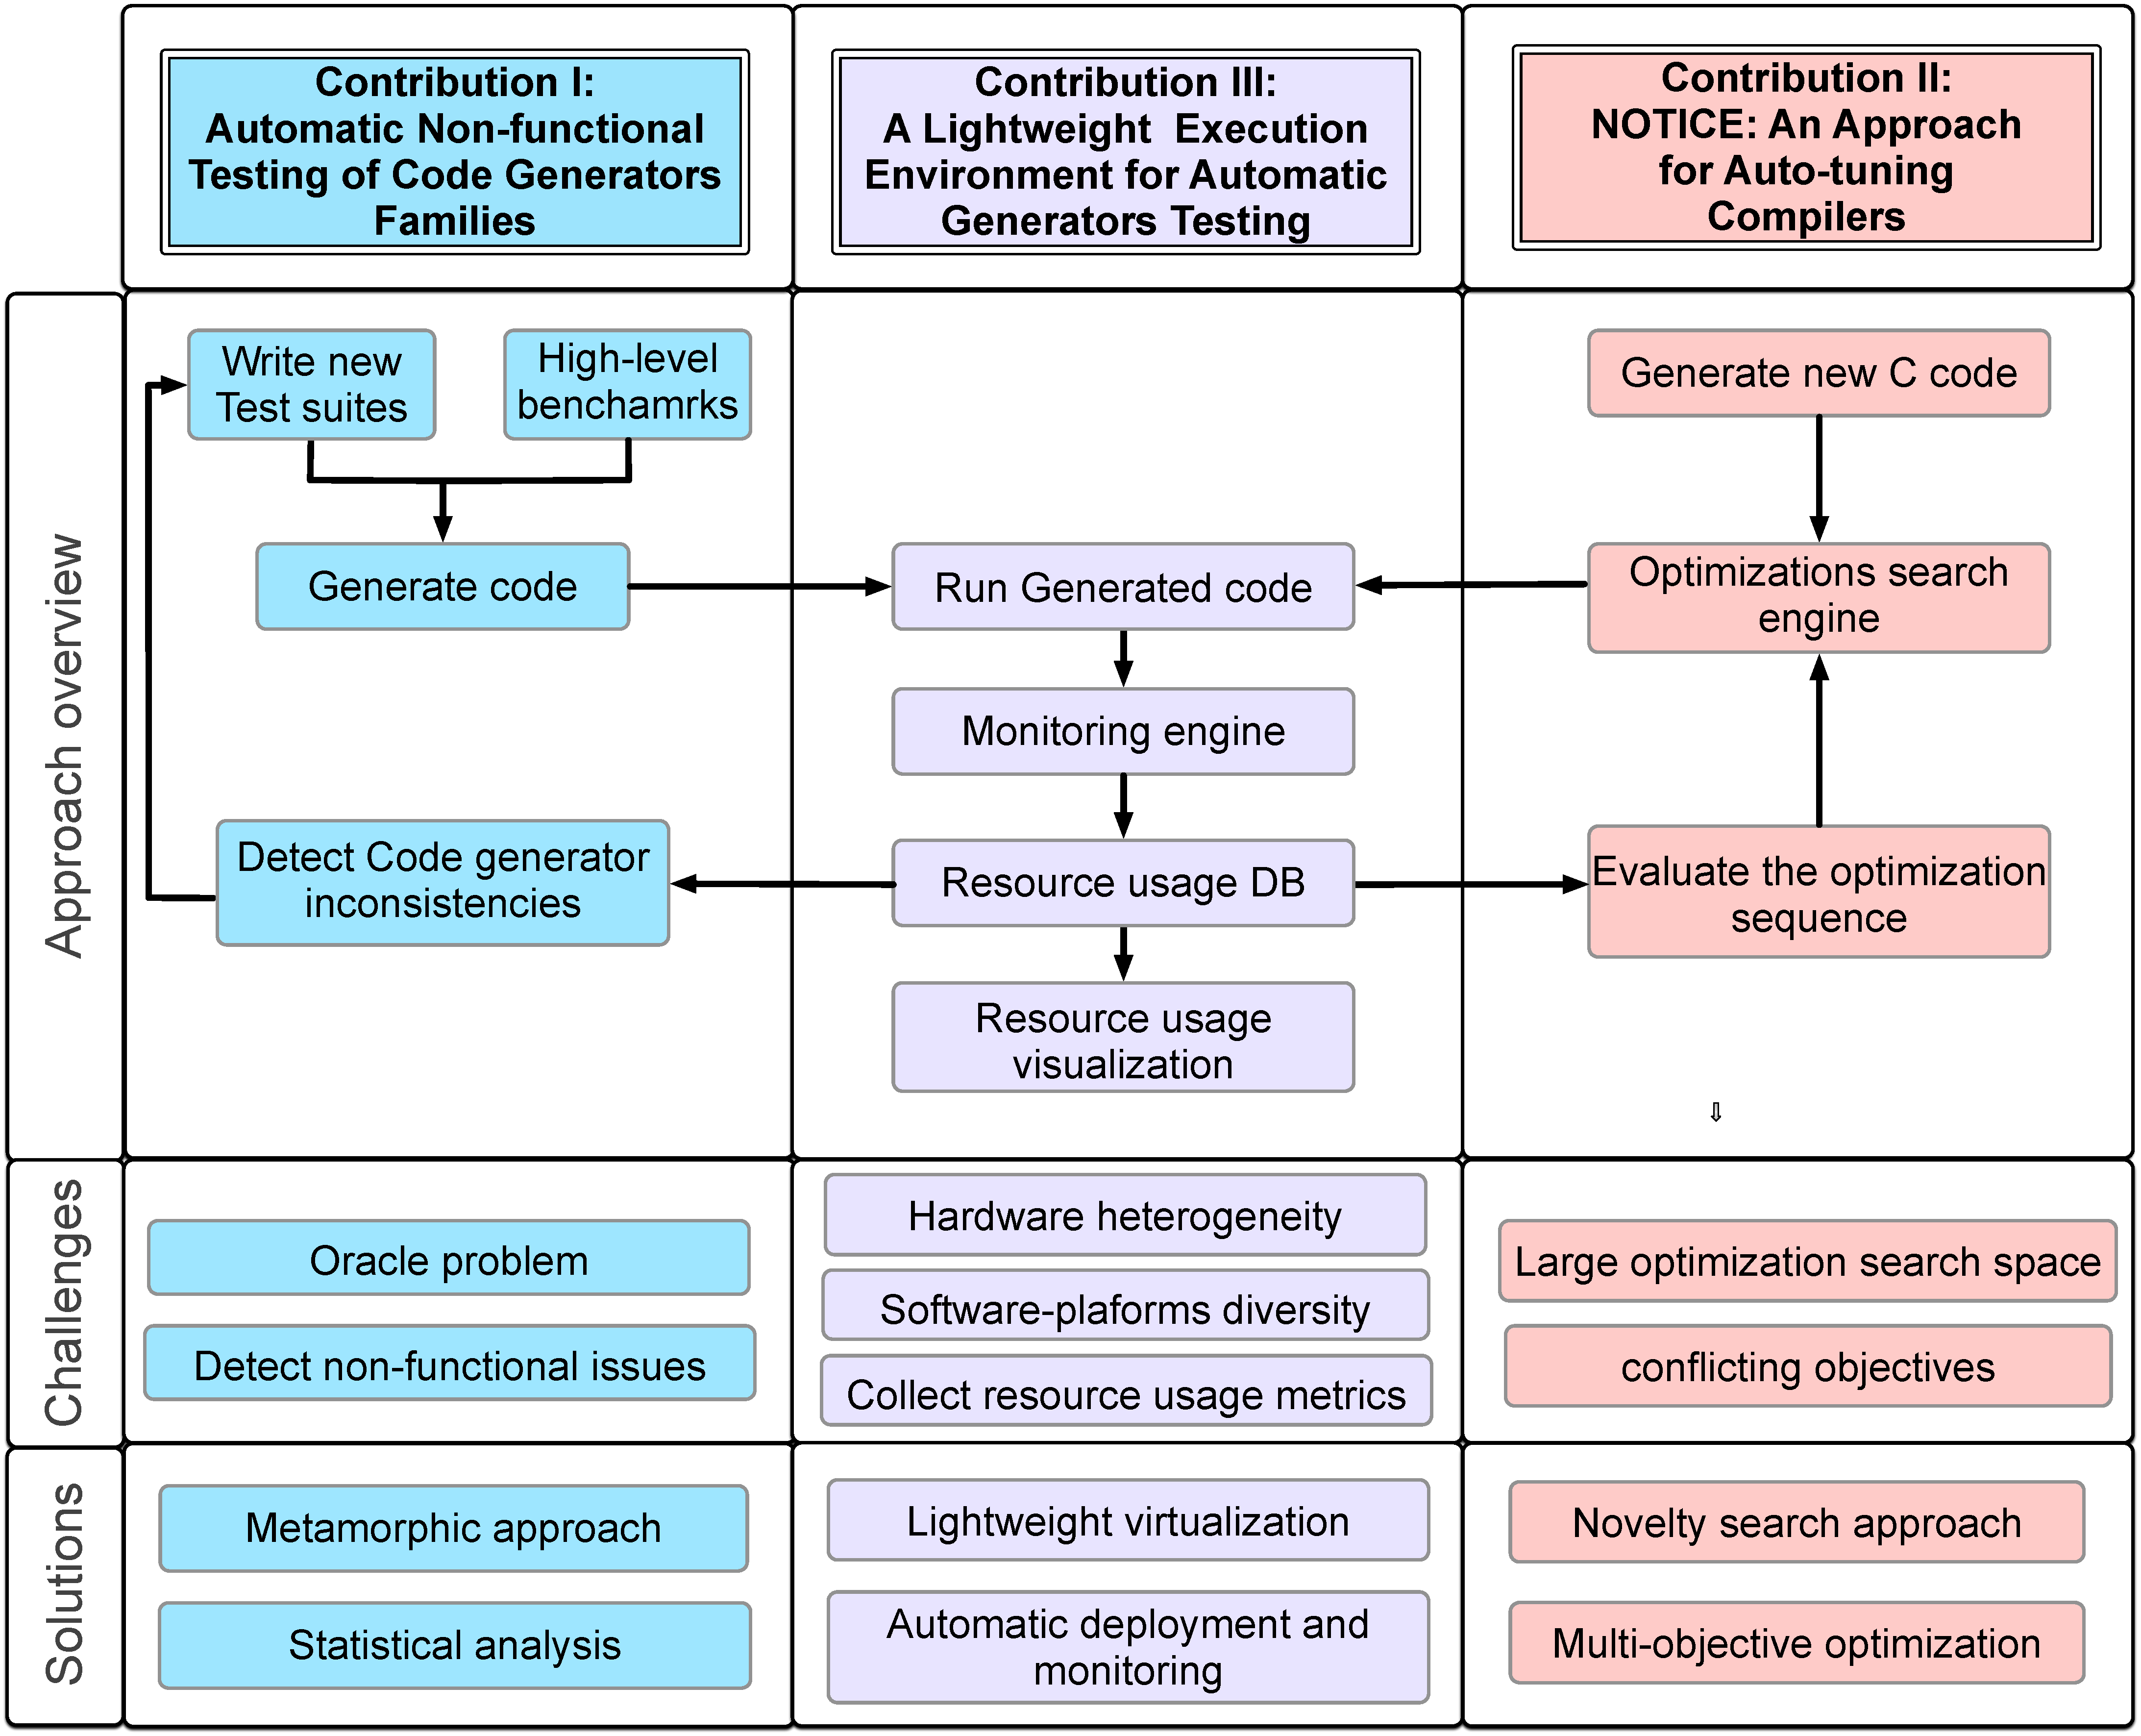
\includegraphics[scale=0.23]{Chapitre0/fig/overview}
	\caption{Summary of contributions}
	\label{fig:overview}
\end{figure}

This thesis makes three main contributions:
\begin{itemize}
	\item \textbf{Contribution I: Automatic non-functional testing of code generators families (in blue): }
	
	In this contribution (Chapter \ref{chap:code generators}), we propose an approach for automatic non-functional  testing of code generators. As discussed earlier, existing solutions lack of automation and efficiency to find code generator issues. Particularly, the problem of non-functional testing as well as the test oracle definition are not addressed. In this contribution, we address the limitations of the state of the art by describing an approach based on metamorphic testing and statistical analysis to efficiently detect inconsistencies within code generator families.
	Thus, starting from high-level benchmarks and test suites, we generate automatically source code to five different target languages (\ie, using a code generator family). We execute the generated code and evaluate the resource usage metrics using the lightweight testing infrastructure presented in the contribution III. Inconsistencies are then reported for further inspection.  
	
	\item \textbf{Contribution II: NOTICE, An approach for auto-tuning compilers (in red):}
	
	As discussed in the state of the art, there are two main limitations we would address: the problem of exploring the large optimization search space and the multi-objective exploration for finding trade-offs between conflicting objectives. 
	Thus, we present in Chapter \ref{chap:compilers}, an adaptation of the novelty search algorithm for compilers auto-tuning. Our contribution focuses on tuning GCC compilers based on randomly generated C programs.
	This approach shares the same monitoring infrastructure as the previous contribution in order to evaluate the impact of discovered optimization sequences on resource usage. The outcome of this approach is the best set of optimizations sequences for a giving hardware architecture, for a given input program and for a specific resource usage metric. We also provide a multi-objective optimization evaluation to tackle the problem of conflicting objectives.
	
	\item \textbf{Contribution III: A lightweight execution environment for software testing and monitoring (in purple):}
	
	We propose in Chapter \ref{chap:docker}, a common infrastructure used by both previous contributions to automate software testing and monitoring. Particularly, it serves as a lightweight execution environment to mimic real software and hardware settings, required to run the generated code. It is based on micro-services namely Docker in order to automate the software deployment, execution and monitoring. It is used by the first both contributions to provide information about the quality of the generated code in terms of memory and CPU usage. Finally, we provide in this contribution a mechanism to visualize at runtime the resource usage of running programs. This contribution address the limitations of the state of the art, namely the lack of solutions that handle the software and hardware requirements when testing/tuning generators.
\end{itemize}

The validation of each contribution is presented in the corresponding chapter. Different experiments are used to illustrate the characteristics of each solution we present.




\chapter{Automatic non-functional testing of code generators families}

Generative software development has paved the way to the creation of numerous code generators that automatically translate high-level system specifications into multi-target executable code.
To preserve software reliability and quality, generated code has to be tested with the same effort as for the manually written code. 
Any issue with code generators should be detected and corrected as early as possible in order to ensure the correct behavior of delivered software.
We presented in Chapter \ref{chap:SOTA} several approaches that address the automatic functional testing of code generators. However, automatically testing the non-functional properties of generated code remains a challenging task that has not been addressed yet.

This chapter describes a testing approach that automatically detects anomalies in code generators in terms of non-functional properties (\ie, resource usage and performance). In fact, we adapt the idea of metamorphic testing to the problem of code generators testing. Hence, our approach relies on the definition of high-level test oracles (\ie, metamorphic relations) to check the potential inefficient code generator among a family of code generators. Moreover, we apply different statistical methods in order to automate the inconsistencies detection.
We evaluate our approach by analyzing the performance of Haxe, a popular high-level programming language that involves a set of cross-platform code generators. 
Experimental results show that our approach is able to detect some performance inconsistencies that reveal real issues in Haxe code generators.

This chapter is organized as follows: 

%Section \ref{sec:cg_introduction} introduces the context of this work, \ie, the non-functional testing of code generators.

Section \ref{sec:cg_Motivation} presents the motivations behind this work. In particular, we discuss three motivation examples and the challenges we are facing.

Section \ref{sec:trad} presents the traditional process for non-functional testing of a code generator family.


Section \ref{sec:cd_approach} describes the general approach overview and the testing strategy.

In Section \ref{sec:cg_evaluation}, the evaluation and results of our experiments are discussed. Hence, we provide more details about the experimental settings, the code generators under test, the benchmark used, the evaluation metrics, etc. We discuss then the evaluation results.

Finally, we conclude in Section \ref{sec:cg-conclusion}. 

\iffalse
\section{Introduction}
\label{sec:cg_introduction}

Generative programming techniques become a common practice for software development to tame the runtime platform heterogeneity that exists in several domains such as mobile or Internet of Things development. 
The main benefit of using generative programming is to reduce the development and maintenance effort, allowing the development at a higher-level of abstraction through the use of Domain-Specific Languages (DSLs)~\cite{brambilla2012model} for example. 
DSLs, as opposed to general-purpose languages, are high-level software languages that focus on specific problem domains. 
DSLs or models are generally coupled with the use of code generators that will automatically transform the manually designed models to software artifacts, which can be deployed on different target platforms. 

However, code generators are known to be very difficult to implement and maintain since they involve a set of complex and heterogeneous technologies~\cite{france2007model,guana2015developers}.
To preserve software reliability and quality, code generators have to respect different requirements. In fact, \textit{non-mature} code generators can generate defective software artifacts which range from uncompilable or semantically dysfunctional code that causes serious damage to the generated software; to non-functional bugs which lead to poor-quality code that can affect system reliability and performance (\eg, high resource usage, high execution time, etc.). 
As a matter of fact, these defects (or also anomalies) should be detected and corrected as early as possible in order to ensure the correct behavior of delivered software.
To check the correctness of the code generation process, developers often define (at design or runtime level) a set of test cases that will verify the functional behavior of generated code. 
After code generation, test suites are executed within each target platform, which may lead to either a correct behavior (\ie, expected output) or incorrect one (\ie, failures, errors).
However, the functional correctness of generated code is not enough to claim the effectiveness of code generators. Properties such as memory usage and performance are very important to evaluate. In some cases, the quality of the generated code can negatively influence on the non-functional requirements and cause performance issues\cite{hundt2011loop,ray2014large}.

Testing the non-functional properties of code generators is a challenging and time-consuming task because developers need to deploy and run code every time a change is made in order to analyze and verify its non-functional behavior.
This task becomes more tedious when targeting different platforms and software languages. Thus, different platform-specific tools will be needed to track bugs and identify the cause of execution failures~\cite{guana2014chaintracker,delgado2004taxonomy}. 
As stated in the state of the art, there is a lack of automatic solutions that check the non-functional issues such as the properties related to the resource consumption of generated code (Memory or CPU consumption).

%we propose a testing approach based on a runtime monitoring infrastructure to automatically check the potential inefficient code generators. This infrastructure, based on system containers as execution platforms, allows code-generator developers to evaluate the generated code performance. %In fact, we provide a fine-grained understanding of resource consumption and analysis of components behavior. 


In this chapter, we are presenting the following contributions:

\begin{itemize} 	
	
	\item We propose a fully automated black-box testing approach for detecting code generator inconsistencies within code generator families. We use metamorphic relations as means of test oracles for our test suites. 
	Statistical methods are applied to define these metamorphic relations.
	In this contribution, we focus on detecting anomalies related to performance and resource usage properties. 
	
	\item We report the results of an empirical study by evaluating the non-functional properties of the Haxe code generators. 
	Haxe is a popular high-level programming language\footnote{\num{1892} GitHub stars} that involves a set of cross-platform code generators able to generate code to different target platforms. The obtained results provide evidence to support the claim that our proposed approach is able to detect code generator issues.
	

	
\end{itemize}
\fi
\section{Context and motivations}
\label{sec:cg_Motivation}

\subsection{Code generator families}
Today, different customizable code generators can be used to easily and efficiently generate code for different software platforms, programming languages, operating systems, etc. This work is based on the intuition that a code generator is often a member of a family of code generators\cite{chae2008building}.

\begin{mydef}[\textbf{Code generator family}]
	We define a code generator family as a set of code generators that takes as input the same language/model and generate code for different target software platforms.
\end{mydef}
%Thus, we can automatically compare the performance between different versions
%of generated code (coming from the same source program). Based on this comparison, we can automatically detect singular resource consumptions that could reveal a code generator bug.

For example, this concept is widely used in the industry when applying the \textit{``write once, run everywhere"} paradigm. Users can benefit from a family of code generators (\eg, cross-platform code generators\cite{fumero2015runtime}) to generate from the manually written (high-level) code, different implementations of the same program in different languages. This technique is very useful to address diverse software platforms and programming languages.

As motivating examples for this research work, we can cite three approaches that intensively develop and use code generator families: 
\paragraph{a. Haxe.} 	Haxe\footnote{\url{http://haxe.org/}}~\cite{dasnois2011haxe} is an open source toolkit for cross-platform development which compiles to a number of different programming platforms, including JavaScript, Flash, PHP, C++, C\#, and Java. Haxe involves many features: the Haxe language, multi-platform compilers, and different native libraries. The Haxe language is a high-level programming language which is strictly typed. This language supports both, functional and object-oriented programming paradigms. It has a common type hierarchy, making certain API available on every target platform. Moreover, Haxe comes with a set of code generators that translate manually-written code (in Haxe language) to different target languages and platforms.  
%Haxe code can be compiled for applications running on desktop, mobile, and web platforms. Compilers ensure the correctness of user code in terms of syntax and type safety. Haxe comes also with a set of standard libraries that can be used on all supported targets and platform-specific libraries for each of them. One of the main uses of Haxe is to develop cross-platform games or cross-platform libraries that can run on mobile, on the Web or on a Desktop.  
This project is popular (more than \num{1440} stars on GitHub).

\paragraph{b. ThingML.} ThingML\footnote{\url{http://thingml.org/}} is a modeling language for embedded and distributed systems~\cite{fleurey2011mde}. The idea of ThingML is to develop a practical model-driven software engineering tool-chain which targets resource-constrained embedded systems such as low-power sensors and microcontroller-based devices. ThingML is developed as a domain-specific modeling language which includes concepts to describe both software components and communication protocols. The formalism used is a combination of architecture models, state machines and an imperative action language. The ThingML tool-set provides a  code generator families  to translate ThingML to C, Java and JavaScript. It includes a set of variants for the C and JavaScript code generators to target different embedded systems and their constraints. 
This project is still confidential, but it is a good candidate to represent the modeling community practices.

\paragraph{c. TypeScript.} TypeScript\footnote{\url{https://www.typescriptlang.org/}}is a typed superset of JavaScript that compiles to plain JavaScript~\cite{rastogi2015safe}. In fact, it does not compile to only one version of JavaScript. It can transform TypeScript to EcmaScript 3, 5 or 6. It can generate JavaScript that uses different system modules ('none', 'commonjs', 'amd', 'system', 'umd', 'es6', or 'es2015')\footnote{Each of this variation point can target different code generators (function \textit{emitES6Module} vs \textit{emitUMDModule} in emitter.ts for example).}. 
This project is popular (more than \num{22478} stars on GitHub).

Functional testing of a code generator family is simple. Since the produced programs are generated form the same high-level program, the oracle can be defined as a comparison between their functional outputs, which should be the same.
In fact, based on the three sample projects presented above, we remark that all GitHub code repositories of the corresponding projects use unit tests to check the correctness of code generators.  

In terms of non-functional tests, we observe that ThingML and TypeScript do not provide any specific tests to check the consistency of code generators regarding the memory or CPU usage properties. Haxe provides two test cases\footnote{https://github.com/HaxeFoundation/haxe/tree/development/tests/benchs} to benchmark the resulting generated code. One serves to benchmark an example in which object allocations are deliberately (over) used to measure how memory access/GC mixes with numeric processing in different target languages. The second test evaluates the network speed across different target platforms.


\subsection{Issues when testing a code generator family}

The main difficulties when testing the resource usage properties of code generators is that we cannot just observe the execution of produced code, but we have to observe and compare the execution of generated programs with equivalent (or reference) implementations (\ie, in other languages). Even if there is no explicit oracle to detect inconsistencies for a single code generator, we could benefit from the family of code generators to compare the behavior of several generated programs and detect singular resource consumption profiles that could reveal a code generator inconsistency~\cite{hundt2011loop}. 

As a consequence, we define a code generator inconsistency as:

\begin{mydef}[\textbf{code generator inconsistency}]
	
	A generated code that exhibits an unexpected behavior in terms of performance or resource usage compared to all equivalent implementations in the same code generator family.
\end{mydef}

The possible issues that can result in code generator inconsistencies can be resumed as following:
\begin{itemize}
	\setlength\itemsep{0em}
	\item  the lack of use of a \textbf{specific function that exists in the standard library} of the target API language  that can speed or reduce the memory consumption of the resulting program.
	\item the lack of use of \textbf{a specific type that exists in the standard library} of the target language  that can speed or reduce the memory consumption of the resulting program.
	\item  the lack of use of\textbf{ a specific language feature in a target language} that can speed or reduce the memory consumption of the resulting program. 
\end{itemize}

Next section discusses the common process used by developers to test the non-functional properties of generated code. We also illustrate how we can benefit from code generator families to identify unexpected behaviors.


%In short, then, we believe that testing the non-functional properties of code generators remains challenging and time-consuming task because developers have to analyze and verify code for each target platform using platform-dependent tools which makes the task of maintaining code generators very tedious. The heterogeneity of platforms and the diversity of target software languages increase the need of supporting tools that can evaluate the consistency and coherence of generated code regarding the non-functional properties. This paper describes a new approach, based on micro-services as execution platforms, to automate and ease the non-functional testing of code generators. This runtime monitoring infrastructure provides a fine-grained understanding of resource consumption and analysis of generated code's behavior.

\section{The traditional process for non-functional testing of a code generator family}
\label{sec:trad}
A reliable and acceptable way to increase confidence in code generators is to validate and check the functional behavior of generated code, which is a common practice in generators testing~\cite{jorges2014back,stuermer2007systematic,sturmer2005overview}.
%Therefore, developers try to check the syntactic and semantic correctness of the generated code by means of different techniques such as static analysis, test suites, etc., and ensure that the code is behaving correctly.  
However, proving that the generated code is functionally correct is not enough to claim the effectiveness of the code generator under test. 

In fact, code generators have to respect different requirements to preserve software reliability and quality~\cite{demertzi2011analyzing}. 
In this case, ensuring the quality of generated code requires examining several non-functional properties such as code size, resource or energy consumption, execution time, etc~\cite{pan2006fast}.
%A \textit{non-mature} code generator might generate defective software artifacts (code smells) that violates common software engineering practices, resulting in a poor-quality code that can affect system reliability and performance (\eg, high resource usage, high execution time, etc.).
Figure \ref{fig:bbackground.pdf} summarizes the classical steps required to ensure the code generation and non-functional testing of a code generator family. 
We distinguish four major steps: software design using high-level system specifications, code generation, code execution, and non-functional testing of generated code. 


\begin{figure*}[t]
	\center
	
	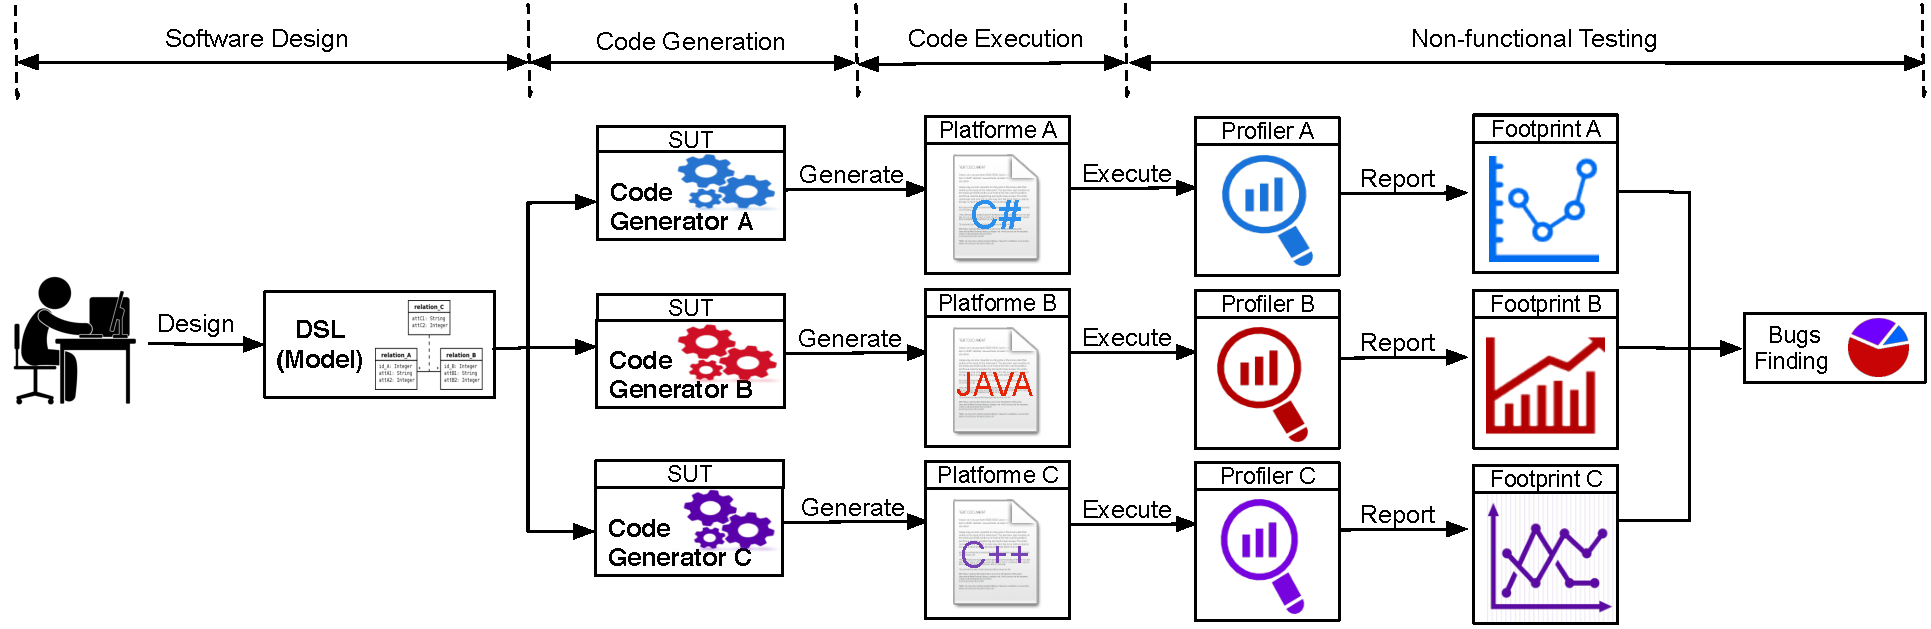
\includegraphics[width=1.\linewidth]{chapitre4/fig/background.pdf}
	\caption{An overall overview of the different processes involved to ensure the code generation and non-functional testing of produced code from design time to runtime: the classical way}
	\label{fig:bbackground.pdf}
\end{figure*}


In the first step, software developers have to define, at design time, the software's behavior using a high-level abstract language (DSLs, models, program, etc). Afterwards, developers can use platform-specific code generators to ease the software development and automatically generate code for different languages and platforms. We depict, as an example in Figure \ref{fig:bbackground.pdf}, three code generators from the same family capable to generate code to three software programming languages (Java, C\# and C++). The first step is to generate code from the previously designed model.
% Transformations from model to code within each code generator might be different and may integrate different transformation rules. As an example, we distinguish model-to-model transformations languages such as ATL~\cite{jouault2005transforming} and template-based model-to-text transformation languages such as Acceleo~\cite{musset2006acceleo} to translate high-level system specifications into executable code and scripts~\cite{bragancca2008transformation,czarnecki2003classification}. The main task of code generators is to transform models to general-purpose and platform-dependent languages.
Afterwards, generated software artifacts (\eg, Java, C\#, C++, etc.) are compiled, deployed and executed across different target platforms (\eg, Android, ARM/Linux, JVM, x86/Linux, etc.). 
%Thus, several code compilers are needed to transform source code to machine code (binaries) in order to get executed. 
Finally, to perform the non-functional testing of generated code, developers have to collect, visualize and compare information about the performance and efficiency of running code across the different platforms. 
Therefore, they generally use several platform-specific profilers, trackers, instrumenting and monitoring tools in order to find some inconsistencies or bugs during code execution~\cite{guana2014chaintracker,delgado2004taxonomy}. Finding inconsistencies within code generators involves analyzing and inspecting the code and that, for each execution platform. For example, one way to handle that, is to analyze the memory footprint of software execution and find memory leaks~\cite{nethercote2007valgrind}. Developers can then inspect the generated code and find some fragments of the code-base that have triggered this issue. %Such non-functional error could occur when the code generator produces code that presents for example: incorrect typing, faulty memory management, code-smells, etc. 
Then, they report this information in order to fix, refactor, and optimize the code generation process. Compared to this classical (and manual) testing approach, our proposed work seeks to automate the last three steps: the code generation and execution on top of different software platforms, and the detection of non-functional issues.


\section{Approach overview}
\label{sec:cd_approach}
Our contributions in this work are divided into two parts:
\begin{itemize}
	\item First, we describe our infrastructure for resource usage monitoring. 
	This contribution addresses the problem of software diversity and hardware heterogeneity, as discussed in Chapter \ref{chap:background}.
	
	\item Second, we present a methodology for automatic detection of inconsistencies in code generator families. This approach addresses the oracle problem when testing the non-functional properties.
\end{itemize}


\subsection{An infrastructure for non-functional testing using system containers}
\label{sec:cg-An infrastructure for non-functional testing using system containers}
In this contribution, we focus on evaluating the non-functional properties related to the resource usage and performance of generated code. To do so, many system configurations (\ie, execution environments, libraries, compilers, etc.) must be taken into account to efficiently generate and test code. 

However, tuning different applications (\ie, generated code) with different configurations on one single machine is complex. A single system has limited resources and this can lead to performance regressions. Moreover, each execution environment comes with a collection of appropriate tools such as compilers, code generators, debuggers, profilers, etc. Therefore, we need to deploy the test harness, \ie, the produced binaries, on an elastic infrastructure that provides facilities to the code generator developers to ensure the deployment and monitoring of generated code in different environment settings. 
Consequently, the testing infrastructure provides support to automatically:
\begin{enumerate}
	\item Deploy the generated code, its dependencies, and its execution environments
	\item Execute the produced binaries in an isolated environment 
	\item Monitor the execution 
	\item Gather resource usage metrics (CPU, Memory, etc.)
\end{enumerate}

To ensure these four main steps, we rely on system containers~\cite{soltesz2007container} as a dynamic and configurable execution environment for running and evaluating the generated programs in terms of resource usage.

\begin{figure*}[h]
	\center
	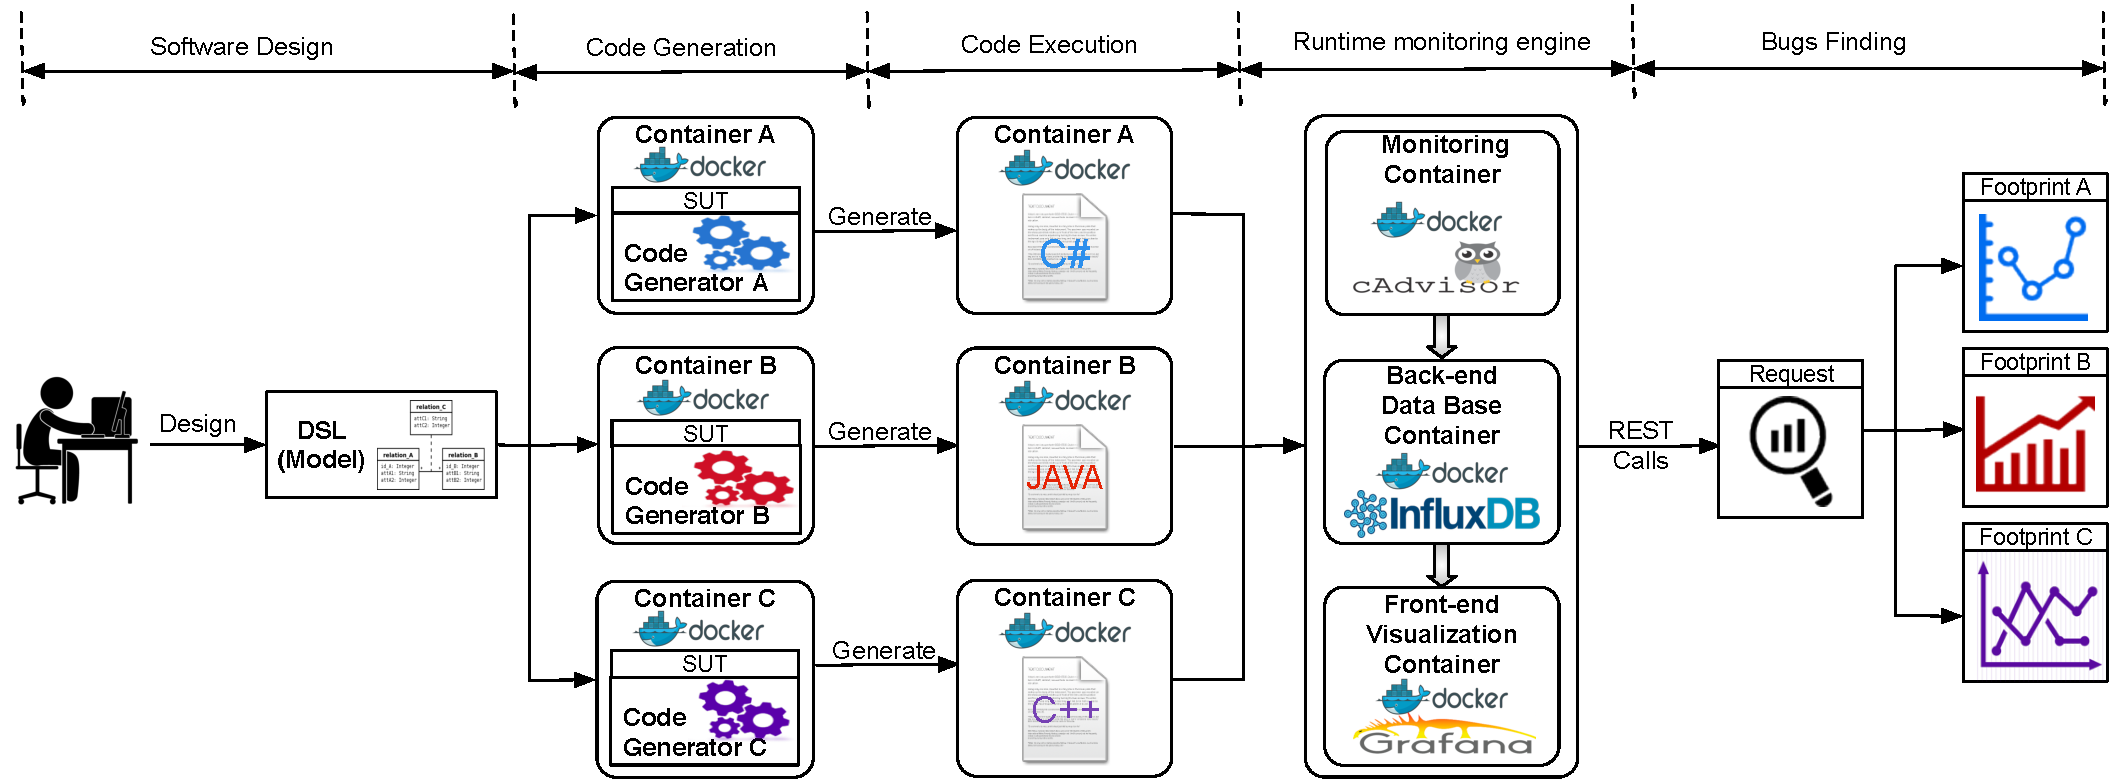
\includegraphics[width=1.\linewidth]{chapitre5/fig/docker_background2.pdf}
	\caption{A technical overview of the different processes involved to ensure the code generation and non-functional testing of produced code from design time to runtime.}
	\label{fig:cg-infra}
\end{figure*}

Figure \ref{fig:cg-infra} shows the container-based infrastructure used for testing code generators. Compared to the classical method presented in Figure \ref{fig:bbackground.pdf}, we add the following features: 
\begin{itemize}
	\item[--] At the code generation level: Code generators are configured inside different containers in order to generate code for the target platform.
	\item[--] At the code execution level: Libraries, compilers and different dependencies are configured in different containers in order to execute the generated code. For each target platform, a new instance is created.
	\item[--] At the non-functional testing level: We add a runtime monitoring engine (based on containers) in order to extract the resource usage properties.
\end{itemize}

Chapter \ref{chap:docker} provides more details about the technical choices we have made to synthesize this testing infrastructure.

\subsection{A metamorphic testing approach for automatic detection of code generator inconsistencies}
We discussed in Section \ref{sec:cg-Summary: oracle definition approaches} several approaches proposed by the software testing community in order to alleviate the oracle problem. Among the attractive approaches that can be applied to test code generators, we distinguish the metamorphic testing approach (derived oracles). In the following, we describe the basic concept of metamorphic testing and our adaptation of this method to test code generator families in terms of resource usage and performance.

\subsubsection{Basic concept of metamorphic testing}
In this section, we shall introduce the basic concept of metamorphic testing (MT), proposed by Chen \etal \cite{chen1998metamorphic}. The idea of MT is to derive test oracles from the relation between test cases' outputs instead of reasoning about the relation between test inputs and outputs. 

MT recommends that, given one or more test cases (called ``source test cases", ``original test cases", or ``successful test cases") and their expected outcomes (obtained through multiple executions of the target program under test), one or more follow-up test cases can be constructed to verify the necessary properties (called Metamorphic Relations MRs) of the system or function to be implemented. In this case, the generation of the follow-up test cases and verification of the test results require the respect of the MR.

%For example, let \textit{sine} be a function implementing a specification \textit{S}. Let \textit{D} represent the input domain which represents the input values for which we would calculate the \textit{sine}. Usually, the testing process should verify if the \textit{sine(x) = S(x)} $\forall$ \textit{x} $\in$ \textit{D}. The procedure through which the testing program can check whether \textit{sine(x) = S(x)} is called an oracle.
%Automatically generating  \textit{D} (test data) and executing test cases in this example is simple. It consists in generating random numerical values for example. However, it is impossible to do an exhaustive testing to automatically check the expected output.
%For instance, only the special input values  \textit{0}, $\pi/4$,  $\pi/2$, etc., could be the standard test cases since the output of  \textit{sine(x)} for these test data values is known and can be automatically checked against the specification. Nevertheless, special values cannot give us enough confidence in the correctness of the program on more complex or random inputs. 
%Other examples include, testing programs calculating numerical functions or solving complex equations, testing programs that calculate combinatorial problems, testing graphical user interfaces, etc.
%Supposing that the \textit{sine} function is defined using a high level language. The generated \textit{sine} function should be evaluated with the same effort as the manual written code in order to verify whether the code generator has introduced bugs or not.

The classical example of MT is that of a program that computes the \textit{sin} function. A useful metamorphic relation for \textit{sin} functions is $\textit{sin(x) = sin($\pi$ - x)}$. Thus, even though the expected value for the source test case \textit{sin(50)} for example in not known, a follow-up test case can be constructed to verify the MR defined earlier. In this case, the follow-up test case is $\textit{sin($\pi$ - 50)}$ which must produce an output value that is equal to the one produced by the original test case \textit{sin(50)}. If this property is violated, then a failure is immediately detected.
MT generates follow-up test cases as long as the metamorphic relations are respected.
This is an example of a metamorphic relation: an input transformation that can be used to generate new test cases from existing test data, and an output relation MR, that compares the outputs produced by a pair of test cases.
MR can be any properties involving the inputs and outputs of two or more executions of the target program such as equalities, inequalities, convergence constraints, and many others.

Because MT checks the relation among several executions rather than the correctness of individual outputs, it can be used to fully automate the testing process without any manual intervention. 
However, constructing the metamorphic relations is typically a manual task that demands thorough knowledge of the program under test. It also depends on the application context and domain. 
The effectiveness of metamorphic testing is highly dependent on the identified metamorphic relations, and designing effective metamorphic relations is thus a critical step when applying metamorphic testing.

We describe in the next section our adaptation of MT to the problem of non-functional testing of code generators families.

\subsubsection{Adaptation of the MT approach to detect code generator inconsistencies}
In general, MT can be applied to any problem in which a necessary property involving multiple executions of the target function can be formulated. Some examples of successful applications are presented in \cite{zhou2004metamorphic}. We note that MT is recently applied to compilers testing\cite{donaldson2016metamorphic,tao2010automatic,le2014compiler}.

To apply MT, there are four basic steps to follow:

\begin{enumerate}
 \item Find the properties of the system under test: the system should be investigated manually in order to find intended MRs defining the relation between inputs and outputs. This is based on the source test cases.
 \item Generate/select test inputs that satisfy the MR: this means that new follow-up test cases must be generated or selected in order to verify their outputs using the MR.
 \item Execute the system with the inputs and get outputs: original and follow-up test cases are executed in order to gather their outputs.
 \item Check whether these outputs satisfy the MR, and if not, report failures.
\end{enumerate}

We develop now these four points in details to show how we can adapt the MT approach to the code generator testing problem. 
\subsubsection[(Step 1)]{Metamorphic relation }

Step 1 consists in identifying the necessary properties of the program under test and represent them as metamorphic relations. As already stated, a metamorphic relation is a relation derived from different system executions.
We use the MR definition as presented in \cite{tao2010automatic,chan2006integration}:

\begin{mydef}[\textbf{Metamorphic relation}]

Let $(x_{1}, x_{2},..., x_{k})$ be a series of inputs to a function $f$, where $k$ $\geqslant$ 1, and $(f(x_{1}, x_{2},..., x_{k})$ be the corresponding series of results. Suppose $(f(x_{i1}), f(x_{i2}),..., f(x_{im}))$ is a subseries, possibly an empty subseries, of $(f(x_{1})$, $f(x_{2})$,..., $f(x_{k}))$. Let $(x_{k+1}, x_{k+2},..., x_{n})$ be another series of inputs to $f$, where $n \geqslant k+1$, and $(f(x_{k+1})$, $f(x_{k+2})$,..., $f(x_{xn}))$ be the corresponding series of results. Suppose, further, that there exists relations $r(x_{1}$, $x_{2}$,..., $x_{k}$, $f(x_{i1})$, $f(x_{i2})$,...., $f(x_{im})$, $x_{k+1}$, $x_{k+2}$,..., $x_{n}))$ and $r'$$(x_{1}$, $x_{2}$,..., $x_{n}$, $f(x_{1}$, $f(x_{2}$,..., $f(x_{n}))$ such that $r'$ must be true whenever $r$ is satisfied. We say that 


\textbf{MR} = {$(x_{1}, x_{2},...,x_{n}, f(x_{1}), f(x_{2}),..., f(x_{n}) \mid$

$r(x_{1}, x_{2},..., x_{k}, f(x_{i1}), f(x_{i2}),...., f(x_{im}), x_{k+1}, x_{k+2},..., x_{n}))$

$\Rightarrow r'(x_{1}, x_{2},..., x_{n}, f(x_{1}), f(x_{2}),..., f(x_{n}))$} 

is a metamorphic relation. When there is no ambiguity, we simply write the metamorphic relation as 	

\textbf{MR}: if $r(x_{1}, x_{2},..., x_{k}, f(x_{i1}), f(x_{i2}),...., f(x_{im}), x_{k+1}, x_{k+2},..., x_{n}))$

then $r'(x_{1}, x_{2},..., x_{n}, f(x_{1}), f(x_{2}),..., f(x_{n})).$

Furthermore, $x_{1}, x_{2},..., x_{k}$ are known as source test cases and $x_{k+1}, x_{k+2},..., x_{xn}$ are known as follow-up test cases
%Let (x1, x2,..., xk) be a series of inputs to a function f , where k > 1, and f(x1), f(x2),..., f(xk) be the corresponding series of results. Suppose f(xi1 ), f(xi2 ),..., f(xim ) is a subseries, possibly an empty subseries, of f(x1), f(x2),..., f(xk). Let xk+1, xk+2,..., xn be another series of inputs to f , where n ≥ k + 1, and f(xk+1), f(xk+2),..., f(xn) be the corresponding series of results. Suppose, further, that there exists relations r(x1, x2, ..., xk, f(xi1 ), f(xi2 ), ..., f(xim ), xk+1, xk+2, ..., xn) and r (x1, x2,..., xn, f(x1), f(x2),..., f(xn)) such that r must be true whenever r is satisfied. We say that MR = { (x1, x2,..., xn, f(x1), f(x2),..., f(xn)) | r(x1, x2,..., xk, f(xi1 ), f(xi2 ),..., f(xim ), xk+1, xk+2,..., xn) → r (x1, x2,..., xn, f(x1), f(x2),..., f(xn)) } is a metamorphic relation. When there is no ambiguity, we simply write the metamorphic relation as MR: If r(x1, x2,..., xk, f(xi1 ), f(xi2 ),..., f(xim ), xk+1, xk+2,..., xn) then r (x1, x2,..., xn, f(x1), f(x2),..., f(xn)). Furthermore, x1, x2, ..., xk are know

\end{mydef}

A code generator family can be seen as a function: $C : I \rightarrow P$, where $I$ is the domain of valid high-level source programs and $P$ is the domain of the target programs that are generated by the different code generators of the same family. The property of a code generator family implies that the generated programs $P$ share the same behavior as it is specified in $I$. 

The availability of multiple generators with comparable functionality allows us to adapt the MT in order to detect non-functional inconsistencies. In fact, if we can find out proper relation $R$ (see equation \ref{eqR}) of the non-functional behavior, we can get the metamorphic relation and conduct MT for testing code generator families.
Let $f(P(t_{i}))$ be a function that calculates the non-functional output (such as execution time or memory usage) of the input test suite ($t_{i}$), running on a generated program ($P$). Since we have different program versions generated in the same family, we denote by $(P_{1}(t_{i})$, $P_{2}(t_{i})$,..., $P_{n}(t_{i}))$ the set of generated programs. The corresponding outputs would be $(f(P_{1})$, $f(P_{2})$,..., $f(P_{n}))$. Thus, our MR looks like this:

\begin{equation}
\label{eqR}
	 R(P_{1}(t_{i}), P_{2}(t_{i}),..., P_{n}(t_{i}))  \Rightarrow R(f(P_{1}(t_{i})), f(P_{2}(t_{i})),..., f(P_{n}(t_{i})))
\end{equation}

On the one hand, we use the following equation $P_{1}(t_{i}) \equiv P_{2}(t_{i})$ to denote \textit{the functional equivalence relation} between two generated programs $P_{1}$ and $P_{2}$ from the same family. This means that the generated programs $P_{1}$ and $P_{2}$ have the same behavioral design, and for any test suite $t_{i}$, they have the same functional output. 
If this relation is not satisfied, then there is at least one faulty code generator that produced incorrect code. In this this work, we focus on the non-functional testing, so we ensure that this relation is ensured by excluding all the programs that do not exhibit the same behavior. 


On the other hand, since we are comparing equivalent implementations of the same program written in different languages, we assume that the memory usage and execution time should be more or less the same with a small variation for each test suite across the different versions. Obviously, we are expecting to get a variation between different executions because we are comparing the execution time and memory usage of test suites that are written in different languages and executed using different technologies (\eg, interpreters for PHP, JVM for Java, etc.). 
This observation is also based on initial experiments, where we evaluate the resource usage/execution time of several test suites across a set of equivalent versions generated using a code generator family (presented in details in the evaluation, Section \ref{sec:cg_evaluation}). As a consequence, we use the notation $\Delta\{f(P_{1}(t_{i})), f(P_{2}(t_{i}))\}$ to designate the variation of memory usage or execution time of test suite execution $t_{i}$ across two versions of generated code $P_{1}$ and $P_{2}$ written in different languages. We suppose that this variation should note exceed a certain threshold value $T$, otherwise, we raise a code generator inconsistency.
Based on this intuition, the MR can be represented as:

\begin{equation}
P_{1}(t_{i}) \equiv P_{2}(t_{i}) \equiv ... \equiv P_{n}(t_{i}) \Rightarrow \Delta\{f(P_{1}(t_{i})), f(P_{2}(t_{i})),..., f(P_{n}(t_{i}))\} < T\quad (n\geqslant 2)
\end{equation}

This MR is equivalent to say that: \textbf{if} a set of functionally equivalent programs are generated using the same code generator family $((P_{1}(t_{i})$, $P_{2}(t_{i})$,...,$P_{n}(t_{i}))$, and with the same input test suite $t_{i}$, \textbf{then} the comparison of their non-functional outputs $(f(P_{1}(t_{i}))$, $f(P_{2}(t_{i}))$,..., $f(P_{n}(t_{i})))$ should be the same while taking into account a tolerance interval defined by the variation $\Delta$ that shall not exceed a specific threshold value $T$.

The generated code that violates this metamorphic property represents an inconsistency and its corresponding code generator is considered as defective.

\subsubsection[(Steps 2, 3, and 4)]{Metamorphic testing}
\label{sec:cg-Metamorphic testing}
\begin{figure}[h]
	\centering
	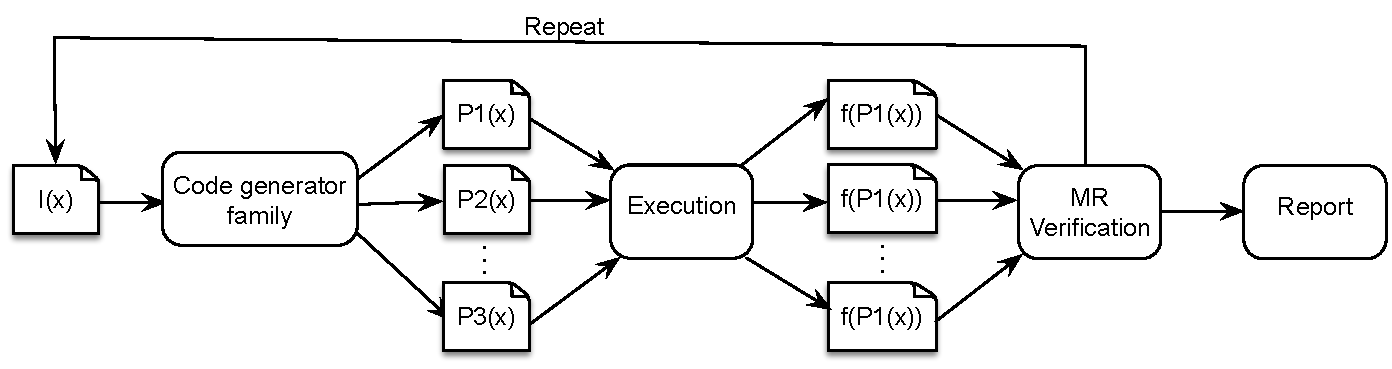
\includegraphics[width=1.\linewidth]{chapitre4/fig/MT}
	\caption{The metamorphic testing approach for automatic detection of code generator inconsistencies}
	\label{fig:cg_MT}
\end{figure}

So far, we have defined the MR necessary for inconsistencies detection. We describe now our automatic metamorphic testing approach based on this relation (steps 2, 3, and 4). 
Figure \ref{fig:cg_MT} shows the approach overview.
The code generator family takes the same input program I and generate a set of equivalent test programs $(P_{1}$, $P_{2}$,...,$P_{n})$. 
This corresponds to step 2. In our MT adaptation, follow-up test cases represent the equivalent test programs that are automatically generated using a code generator family. 
Test suites are also generated automatically since we suppose that they are already defined at design time. In fact, the same test suite (test cases + input data values) is passed to all generated programs. 
Then, generated programs and their corresponding test suites are executed (step 3). Afterwards, we measure the memory usage or execution time of these generated programs $(f(P_{1}(t_{i}))$, $f(P_{2}(t_{i}))$,..., $f(P_{n}(t_{i})))$. Finally, the execution results are compared and verified using the MR defined earlier (step 4).
In this process, inconsistencies will be reported when one of the follow-up equivalent test program violates the MR.





\subsubsection{Variation threshold}
\label{sec:cg-Variation threshold}
One of the questions that may be raised when applying our MT approach is how can we find the right variation threshold $T$ from which an inconsistency is detected? Answering this question is very important to prove the effectiveness of our MT approach.
To do so, we conduct a statistical analysis of our non-functional data in order to find an accurate threshold value $T$.
Before that, the non-functional outputs need to be prepared to make them suitable for the statistical methods employed by our methodology. Thus, we describe first our process for data preparation:

\paragraph{Data preparation}~\\ 
As depicted in Table \ref{tab:Non-functional output results}, each program comes with a set of test suites $(t_{1}$, $t_{2}$,..., $t_{m})$. Evaluating a test suite requires the calculation of the memory usage or execution time $f(P_{1}(t_{i}))$,  $f(P_{2}(t_{i}))$,..., $f(P_{n}(t_{i}))$ where $(1 \leq i \leq m)$  for all target software platforms. Thus, obtained results represent a matrix where columns indicate the non-functional value (raw data) for each target software platform and rows indicate the corresponding test suite.
\begin{table}[h]
	\centering
	
	\begin{tabular}{|c| c |c |c| c|}				
		\hline

		 &  Target platform $1$ &  Target platform $2$ & ... & Target platform $n$  \\ \hline
		$t_{1}$  &  $f(P_{1}(t_{1}))$ &  $f(P_{2}(t_{1}))$ & ... & $f(P_{n}(t_{1}))$  \\ \hline
		$t_{2}$ &  $f(P_{1}(t_{2}))$ &  $f(P_{2}(t_{2}))$ & ... & $f(P_{n}(t_{2}))$  \\ \hline
		... &  ... &  ... & ... & ...  \\ \hline
		$t_{m}$ &  $f(P_{1}(t_{m}))$ &  $f(P_{2}(t_{m}))$ & ... & $f(P_{n}(t_{m}))$  \\ \hline
	\end{tabular}
	
	\caption{Results of test suites execution}
	\label{tab:Non-functional output results}
\end{table}

The non-functional data should be converted into a format that can be understood by our statistical methods. One way to compare these non-functional outputs is to study the factor differences. In other words, we would evaluate for each target platform the number of times (the factor) that a test suite takes to run compared to a reference execution. The reference execution corresponds to the minimum obtained non-functional value of $t_{i}$ execution across the $n$ target platforms. The resulting factor is the ratio between the actual non-functional value and the minimum value obtained among the $n$ versions. The following equation is applied for each cell in order to transform our data:

\begin{equation}
F(f(P_{j}(t_{i})))=\frac{f(P_{j}(t_{i}))}{Min(f(P_{1}(t_{i})),..., f(P_{n}(t_{i})))}  
\end{equation}

The reference execution will automatically get a score value $F = 1$. The maximum value is the one leading to the maximum deviation from the reference execution. For example, let $P_{1}$ be the generated program in Java. If the execution time needed to run $t_{1}$ yields to the minimum value $f(P_{1}(t_{1}))$ compared to other versions, then $f(P_{1}(t_{1}))$ will get a factor value $F$ equal to $1$ and the other versions will be divided by $f(P_{1}(t_{1}))$ to get the corresponding factor values compared to Java.

\paragraph{Statistical analysis}~\\
 
In our MT approach, an inconsistency is a resource usage/performance variation that exceeds a specific threshold value $T$. 
We propose the use of two variation analysis methods\cite{malik2013automatic}: principal components analysis (PCA) and range charts (R-chart). Table \ref{tab:Statistical methods} gives an overview of these two statistical methods.
The key objective of these methods is to evaluate the memory usage and performance variation, and consequently defining an appropriate $T$ value for our MR. 

\begin{table}[h]
	\centering
	
	\begin{tabular}{| l |l |}				
		\hline
		
		\textbf{Technique} &  \textbf{Method}    \\ \hline
	    R-chart &  Define T as a variation between an upper and lower control limit  \\ \hline
		PCA &  A cutoff value of the PC score distances defines the T \\ \hline
	\end{tabular}
	
	\caption{Variation analysis approaches}
	\label{tab:Statistical methods}
\end{table}

\subparagraph{R-Chart}~\\
In this approach, the variation evaluation between the different versions is determined by comparing the non-functional measurements based on a statistical quality control technique called \textit{R-Chart} or \textit{range chart}\cite{malik2013automatic}. 
R-Chart is used to analyze the variation within processes. It is designed to detect changes in variation over time and to evaluate the consistency of process variation.
R-Chart uses control limits (LCL and UCL) to represent the limits of variation that should be expected from a process. LCL denotes the Lower Control Limit and UCL denotes the Upper Control Limit.
 
When a process is within the controlled limits, any variation is normal. It is said that the process is \textbf{in control}. 
Outside limit variations, however, it is considered as deviation and the R-chart is considered as \textbf{out of control} which means that the process variation is not stable. Thus, it tells that there is an inconsistency leading to this high variation deviation (see Figure \ref{fig:cg-rechart}).

In our case, a process represents the $n$ non-functional outputs obtained after the execution of a test suite $t_{i}$. As we defined the MR, the variation within a single process has to be lower than a threshold $T$. In our settings, this variation must be between the LCL and UCL.

\begin{figure}[h]
	\centering
	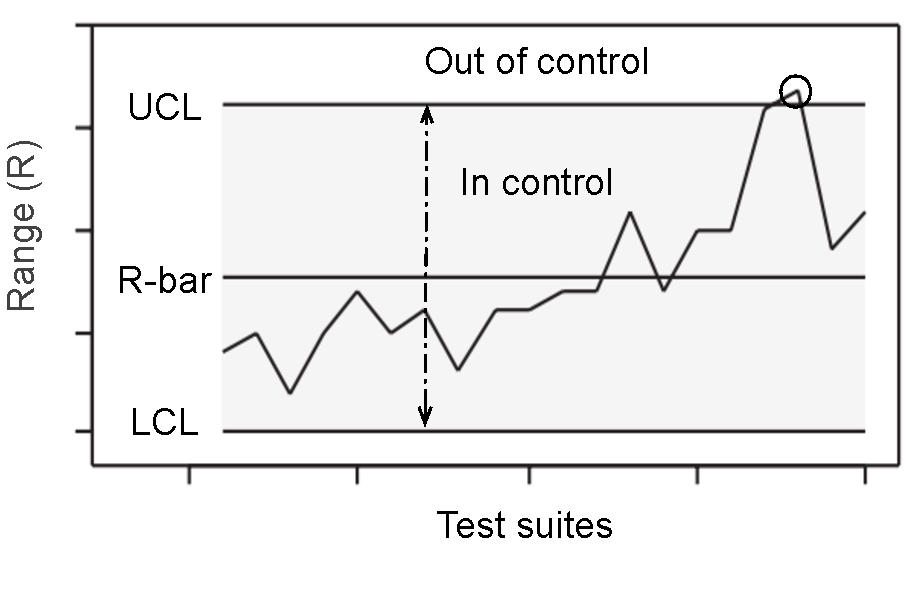
\includegraphics[width=0.6\linewidth]{chapitre4/fig/rchat}
	\caption{The R-Chart process}
	\label{fig:cg-rechart}
\end{figure}

Therefore, for each test suite we calculate the range $R$ corresponding to the difference between the maximum and minimum non-functional outputs across all target platforms.

\begin{equation}
R(t_{i})= Max(f(P_{1}(t_{i})),..., f(P_{n}(t_{i}))) - Min(f(P_{1}(t_{i})),..., f(P_{n}(t_{i})))  
\end{equation}
R quantifies the variation results when running the same test suite $t_{i}$ across different program versions.
To determine whether the variation is in control or not, we need to determine the control limits values. UCL and LCL reflect the actual amount of variation that is observed. Both metrics are a function of R-bar ($\bar{R}$). $\bar{R}$ is the average of R for all test suites.
The UCL and LCL are calculated as follows:
\begin{equation}
\begin{split} 
UCL = D_{4}\bar{R}\\
LCL = D_{3}\bar{R}
\end{split} 
\label{eqUCL}
\end{equation}
where $D_{4}$, $D_{3}$, are control chart constants that depend on the number of variables inside each process (see constants values\footnote{\url{http://www.bessegato.com.br/UFJF/resources/table_of_control_chart_constants_old.pdf}}). 

For example, for a family composed of less than 7 code generators, the $D_{3}$ value is equal to $0$, and as a consequence LCL = $0$. In this case, the UCL represents the threshold $T$ value from which we detect a high variation deviation, leading to an inconsistency. As we stated earlier, the UCL is a function of $\bar{R}$, and $\bar{R}$ is a function of range differences. So, the UCL value (or $T$) is sensitive to new test suites. So, when a new test suite is executed, the $T$ value is updated and the variation is evaluated with the new threshold value. 

We present in the following an alternative statistical approach to analyze the variation of all our data.


\subparagraph{PCA}~\\
With a large number of program versions, the matrix of non-functional data (Table \ref{tab:Non-functional output results}) may be too large to study and interpret the variation properly. There would be too many pairwise correlations between the different versions to consider and the variation is impossible to display (graphically) when test suites are executed in more than three target software platforms.
With 12 variables, for example, there will be more than 200 three-dimensional scatter plots to be designed to study the variation and correlations.
To interpret the data in a more meaningful form, it is therefore necessary to reduce the number of variables composing our data.

Principal Component Analysis\footnote{\url{https://en.wikipedia.org/wiki/Principal_component_analysis}} (PCA) is a multivariate statistical approach that uses an orthogonal transformation to convert a set of observations of possibly correlated variables into a set of values of linearly uncorrelated variables called Principal Components (PCs). It can be applied when data are collected on a large number of variables from a single observation. Thus, we apply the PCA approach to our case study because our dimension space as it is presented in Table \ref{tab:Non-functional output results}, is composed of a set of processes (test suites) where $n$ variables (\eg, target programming languages) are composing each observation. The variability within our model is correlated to these $n$ variables representing the test suites running on $n$ target platforms. 

The main objective of applying PCA is to reduce the dimensionality of the original data and explain the maximum amount of variance with the fewest number of principal components. To do so, PCA is concerned with summarizing the variance-covariance matrix. It involves computing the eigenvectors and eigenvalues of the variance-covariance matrix. The eigenvectors are used to project the data from $n$ dimensions down to a lower dimensional representation. The eigenvalues give the variance of the data in the direction of the eigenvector. The first eigenvector is the vector which defines the direction of maximum variance in the data.
The first principal component is calculated such that it accounts for the greatest possible variance in the data set. The second principal component is calculated in the same way, with the condition that it is uncorrelated with (\ie, perpendicular to) the first principal component and that it accounts for the next highest variance. The eigenvector associated with the largest eigenvalue has the same direction as the first principal component. The eigenvector associated with the second largest eigenvalue determines the direction of the second principal component.
PCA uses many data transformations and statistical concepts. We are not interested in studying all the mathematical aspects of PCA. Thus, we use an existing R package\footnote{\url{http://factominer.free.fr/}} to transform and reduce our data into two PCs in order to visualize the variation of all our data points in a 2-dimensional space.

Our intuition behind the PCA approach is to conduct a general and complete analysis of variation in order to find extreme variation points at the boundaries of the multivariate data. These extreme points represent, from a statistical perspective, \textit{outliers}. Following our MT approach, these points correspond to the inconsistencies (or deviations) we would detect. 
Outliers have an important influence over the PCs. An outlier is defined as an observation which does not follow the model followed by the majority of the data.
One way to detect outliers is to use a metric called Score Distance (SD). SD measures the dispersion of the observations within the PCA space. It thus measures how far an observation lies from the rest of the data within the PCA subspace. 
SD measures the statistical distance from a PC score to the center of the scores. For an observation $x_{i}$ the  score distance is defined as:
\begin{equation}
SD_{i}=\sqrt{\sum_{j=1}^{a} \frac{t_{ij}^{2}}{\lambda_{j}}}
\end{equation}
where $a$ is the number of PCs forming the PCA space, $t_{ij}$ are the elements of the score matrix obtained after running PCA, and $\lambda_{j}$ is the variance of the $j^{th}$ PC which corresponds to the $j^{th}$ eigenvalue.
In order to find the outliers, we compute the 97.5\%-Quantile Q of the Chi-square distribution as a cutoff value of the SD ($\sqrt{\chi_{a,0.975}^{2} }$). It corresponds to a confidence ellipse that covers 97.5\% of the data points. According to the table of the Chi-Square distribution\footnote{\url{https://store.fmi.uni-sofia.bg/fmi/statist/education/Virtual_Labs/tables/tables3.html}}, this value is equal to $\sqrt{7.38}=2.71$.
Any sample whose SD is larger than the cutoff value, is identified as an outliers (or inconsistency). This cut-off value represents the variation threshold $T$ we would define for our MR using the PCA approach.

%It is equal to the squared Mahalanobis distance from the model center to sample i within the score subspace.
%Cut-off values help to distinguish between outliers and regular observations. Any samples whose Mahalanobis distances are larger than the cutoff are identified as the outliers.
%\begin{remark}
%The R-chart method presented earlier, defines a dynamic threshold value (UCL) where follow-up test suites influence on this value. However, using PCA, we are able to analyze the non-functional data of original test suites in order to define a general threshold value (Cutoff) which is steady. Thus, follow-up test suites that exceed this value, causing a high performance or resource usage deviation, are identified as inconsistencies (outliers).
%\end{remark}

We move now to present the evaluation of our approach.


\section{Evaluation}
\label{sec:cg_evaluation}
So far, we have presented an automated approach for detecting inconsistencies within code generator families. So, we shape our goal as this research question:

\textbf{RQ1: } 
\textbf{\textit{How effective is our metamorphic testing approach for automatically detecting inconsistencies in code generator families?}} 

To answer this question, we evaluate the implementation of our approach by explaining the design of our empirical study and the different methods we used to assess the effectiveness of our approach. 
The experimental material is available for replication purposes\footnote{\url{https://testingcodegenerators.wordpress.com/}}.
\subsection{Experimental setup}
\subsubsection{Code generators under test: Haxe compilers}
In order to test the applicability of our approach, we conduct experiments on a popular high-level programming language called Haxe and its code generators. Haxe is an open source toolkit for cross-platform development which compiles to a number of different programming platforms, including JavaScript, Flash, PHP, C++, C\# and Java. Haxe involves many features: the Haxe language, multi-platform compilers, and different native libraries. 
The Haxe language is a high-level programming language which is strictly typed. This language supports both functional programming and object-oriented programming paradigms. It has a common type hierarchy, making certain API available on every targeted platform.
Haxe comes with a set of compilers that translate manually-written code (in Haxe language) to different target languages and platforms. 
Haxe code can be compiled for applications running on desktop, mobile and web platforms. It comes also with a set of standard libraries that can be used on all supported targets and platform-specific libraries for each of them.

The process of code transformation and generation can be described as following: Haxe compilers analyze the source code written in Haxe language. Then, the code is checked and parsed into a typed structure, resulting in a typed abstract syntax tree (AST). This AST is optimized and transformed afterwards to produce source code for the target platform/language.
Haxe offers the option of choosing which platform to target for each program using command-line options. Moreover, some optimizations and debugging information can be enabled through command-line interface, but in our experiments, we did not turn on any further options. 

The Haxe code generators constitute the code generator family we would evaluate in this work.

\subsubsection{Cross-platform benchmark}
One way to prove the effectiveness of our approach is to create benchmarks. Thus, we use the Haxe language and its code generators to build a cross-platform benchmark. The proposed benchmark is composed of a collection of cross-platform libraries that can be compiled to different targets. In these experiments, we consider a code generator family composed of five target Haxe compilers: Java, JS, C++, CS, and PHP code generators. To select cross-platform libraries, we explore github and we use the Haxe library repository\footnote{\url{http://thx-lib.org/}}. So, we select seven libraries that provide a set of test suites with high code coverage scores. 

In fact, each Haxe library comes with an API and a set of test suites. These tests, written in Haxe, represent a set of unit tests that covers the different functions of the API. The main task of these tests is to check the correct functional behavior of generated programs. To prepare our benchmark, we remove all the tests that fail to compile to our five targets (\ie, errors, crashes and failures) and we keep only test suites that are functionally correct in order to focus only on the non-functional properties.
Moreover, we add manually new test cases to some libraries in order to extend the number of test suites. The number of test suites depends on the number of existing functions within the Haxe library.


\begin{table}[h]
	\centering
	
	\begin{tabular}{|c|c|p{8.5cm}|}				
		\hline
		\textbf{Library} & \textbf{\#TestSuites} & \textbf{Description} \\
		\hhline{|=|=|=|}
		Color  &  19 &  Color conversion from/to any color space   \\ \hline
		Core & 51  & Provides extensions to many types  \\ \hline
		Hxmath & 6  & A 2D/3D math library  \\ \hline
		Format  &  4 & Format library such as dates, number formats   \\ \hline
		Promise & 5  & Library for lightweight promises and futures  \\ \hline
		Culture & 5  & Localization library for Haxe \\ \hline
		Math & 5  & Generation of random values \\ \hline
	\end{tabular}
	
	\caption{Description of selected benchmark libraries}
	\label{tab:Description of selected benchmark libraries}
\end{table}

We use then these test suites to transform functional tests into stress tests. This can be useful to study the impact of this load on the resource usage properties of the five target versions. 
We run each test suite 1K times to get comparable values in terms of resource usage.
Table \ref{tab:Description of selected benchmark libraries} describes the Haxe libraries that we have selected in this benchmark to evaluate our approach and the number of test suites used per benchmark.
In total, we have 95 test suites to execute across all benchmark programs.

\subsubsection{Evaluation metrics used}
We evaluate the efficiency of generated code using the following non-functional metrics:

-\textit{Memory usage}:
It corresponds to the maximum memory consumption of the running test suite. Memory usage is measured in \SI{}{\mega\byte}

-\textit{Execution time}:
The execution time of test suites is measured in seconds.

We recall that our testing infrastructure is able to evaluate other non-functional properties of generated code such as code generation time, compilation time, code size, CPU usage. We choose to focus, in this experiment, on the performance (\ie, execution time) and resource usage (\ie, memory usage). Collecting resource usage metrics is ensured by our monitoring infrastructure, presented in Chapter \ref{chap:docker}. 

\subsubsection{Setting up infrastructure}

To assess our approach, we configure our previously proposed container-based infrastructure in order to run experiments on the Haxe case study.
Figure \ref{fig:settingup.pdf} shows a big picture of the testing infrastructure considered in these experiments.

\begin{figure}[h]
	\centering
	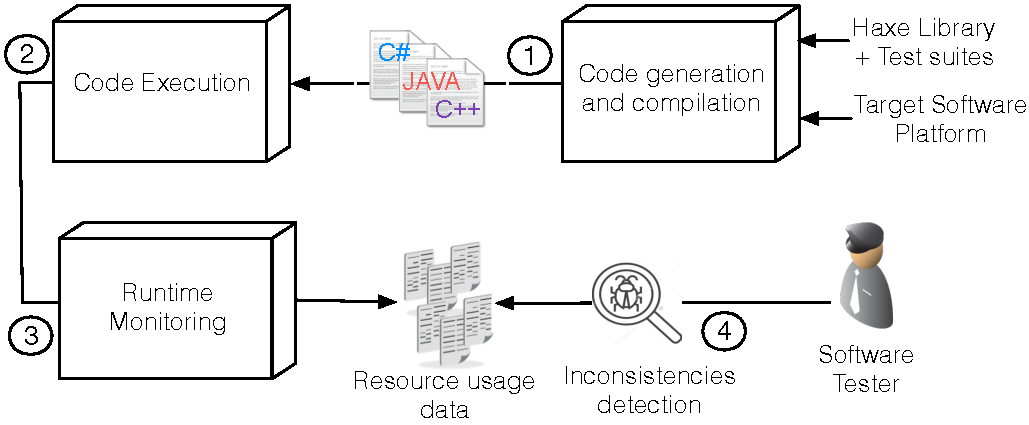
\includegraphics[width=0.7\linewidth]{chapitre4/fig/settingup.pdf}
	\caption{Infrastructure settings for running experiments}
	\label{fig:settingup.pdf}
\end{figure}

First, a first component is created in where we install the Haxe code generators and compilers. It takes as an input the Haxe library we would evaluate and the list of test suites (step 1). It produces as an output the source code files relative to the target software platforms. Afterwards, generated files are compiled (if needed) and automatically executed within the execution container (step 2). This component is a pre-configured container instance where we install the required execution environments such as php interpreter, node (for JS), mono (for C\#), etc. 
In the meantime, while running test suites inside the container, we collect runtime resource usage data (step 3). Chapter \ref{chap:docker}) presents more details about the monitoring engine.
Finally, in step 4, we analyze the non-functional data in order to detect code generator inconsistencies.

\subsection{Experimental methodology and results}
In the following paragraphs, we report the methodology we used to answer \textbf{RQ1} and the results of our experiments. 

\subsubsection{Method}
We now conduct experiments based on the new created benchmark libraries. 
The goal of running these experiments is to observe and compare the behavior of generated code using the defined MR in order to detect code generator inconsistencies.
%We recall, as mentioned in the motivation, that we are not using any oracle function to detect inconsistencies. However, we rely on the comparison results across different targets to detect code generator inconsistencies.

Therefore, we set up, first, our container-based infrastructure as it is presented in Section \ref{sec:cg-An infrastructure for non-functional testing using system containers} in order to generate, execute, and collect the memory usage of our test suites.
Afterwards, we prepare and normalize the gathered data to make it valuable for the statistical analysis. Then, we conduct the R-chart and PCA analysis as described in Section \ref{sec:cg-Variation threshold} in order to analyze the performance and resource usage variations. This will lead us to define an appropriate formula of the MR, used to automatically detect inconsistencies within code generator families (Section \ref{sec:cg-Metamorphic testing}). Finally, we report the inconsistencies we have detected.


%as a quality metric, the standard deviation to quantify the amount of variation among execution traces (\ie, memory usage or execution time) and that, for the five target languages. We recall that the formula of standard deviation is the square root of the variance. Thus, we are calculating this variance as the squared differences from the mean. Our data values in our experiment represent the obtained values in five languages. So, for each test suite we are taking the mean of these five values in order to calculate the variance.
%A low standard deviation of a test suite execution, indicates that the data points (execution time or memory usage data) tend to be close to the mean which we consider as an acceptable behavior.  
%On the other hand, a high standard deviation indicates that one or more data points are spread out over a wider range of values which can be more likely interpreted as a code generator inconsistency. 

\subsubsection{Results}
\paragraph{R-chart results}~\\
\begin{figure}
	\centering  
	\subfigure[R-chart of the Core benchmark program]{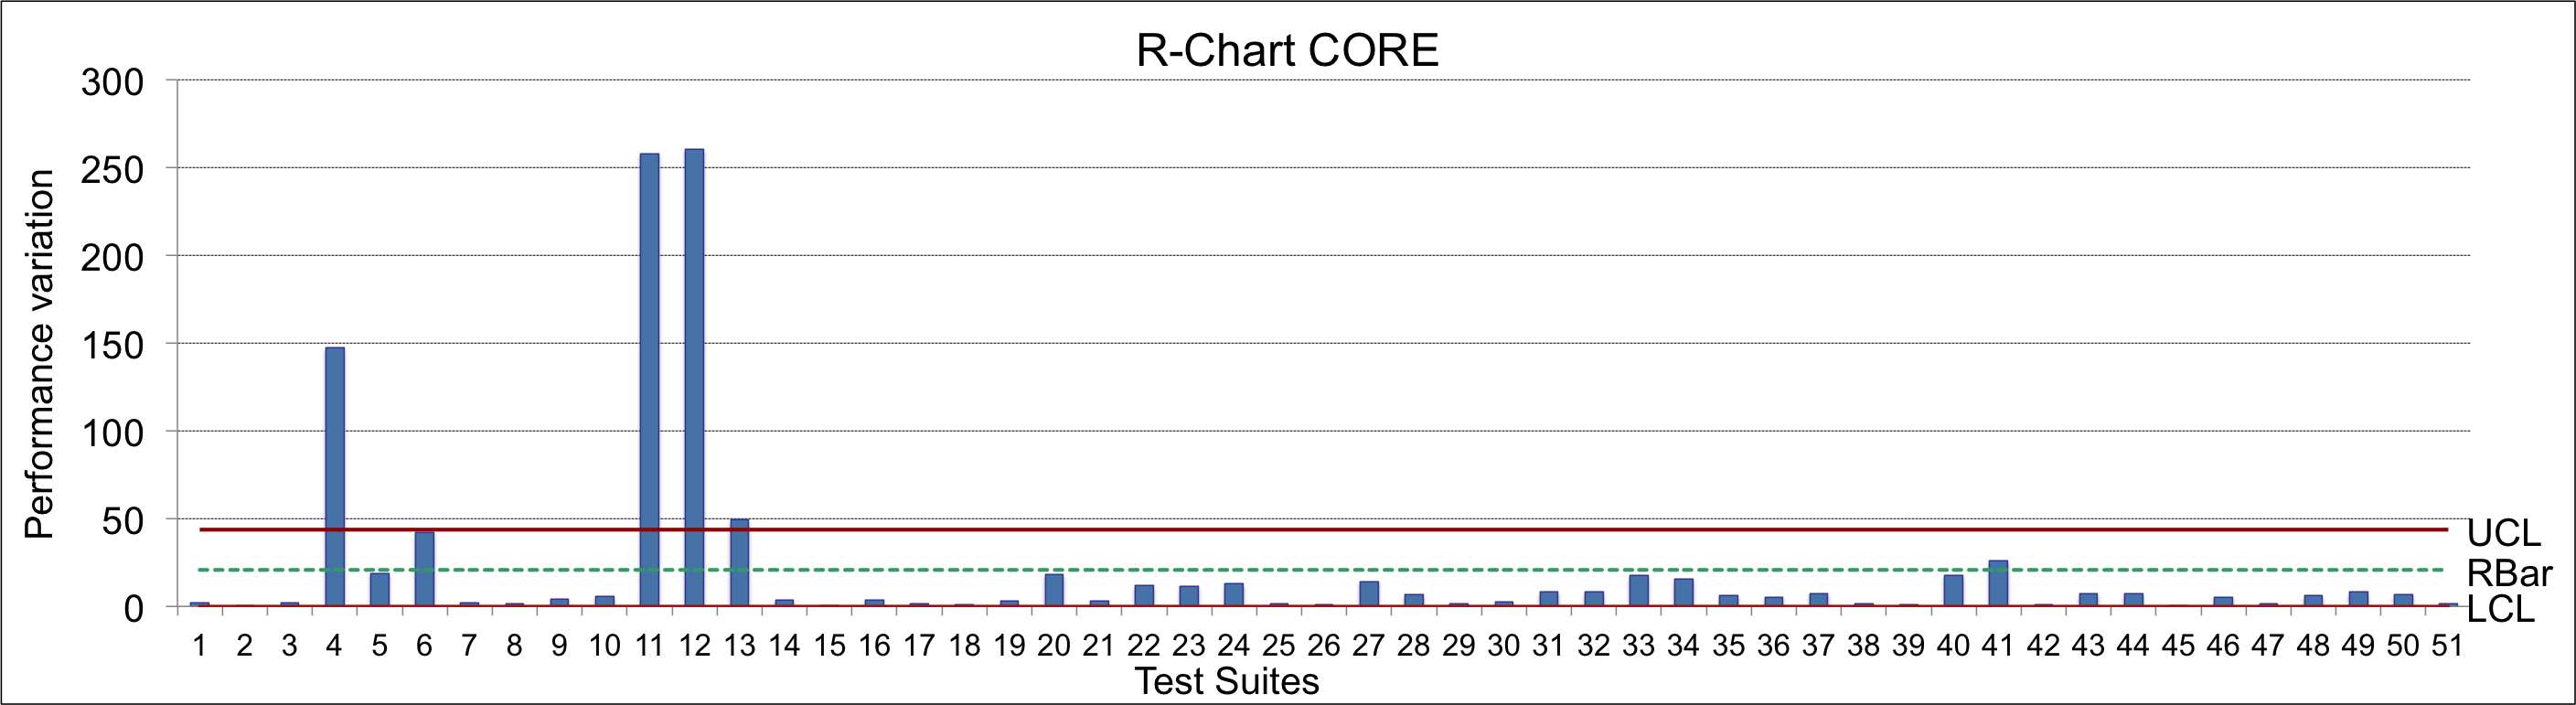
\includegraphics[width=0.96\linewidth]{chapitre4/fig/1.png}\label{rt1}}
	\subfigure[R-chart of the Color benchmark program]{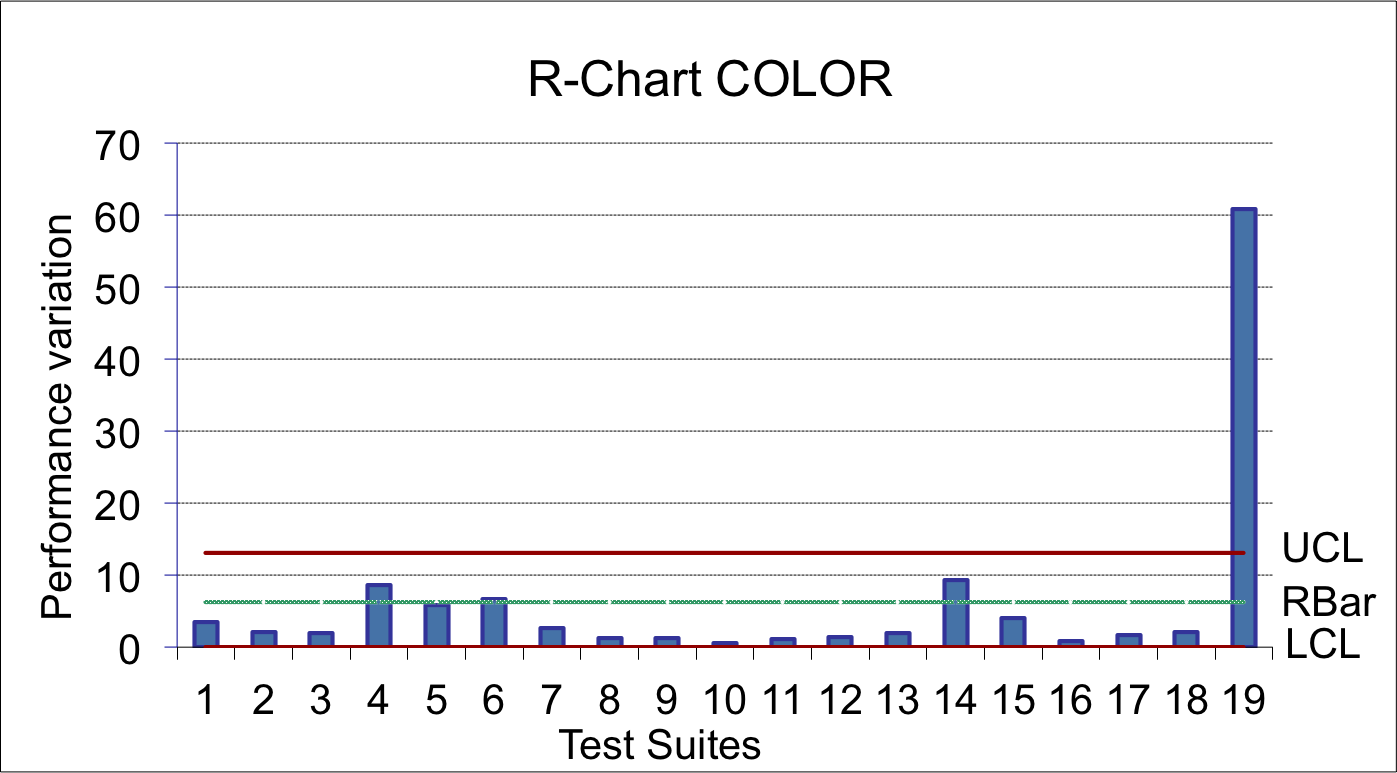
\includegraphics[width=0.48\linewidth]{chapitre4/fig/2.png}\label{rt2}}
	\subfigure[R-chart of the Hxmath benchmark program]{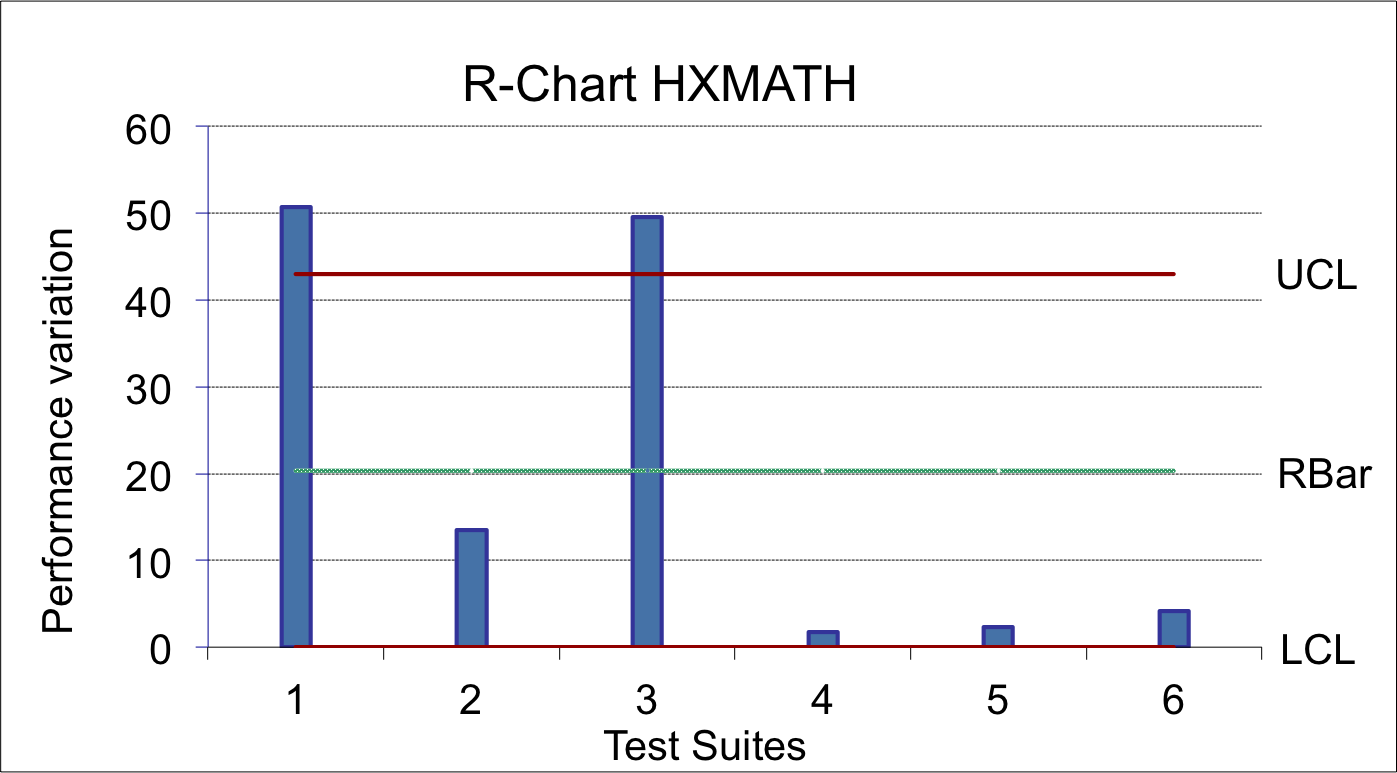
\includegraphics[width=0.48\linewidth]{chapitre4/fig/3.png}\label{rt3}}
	\subfigure[R-chart of the Format benchmark program]{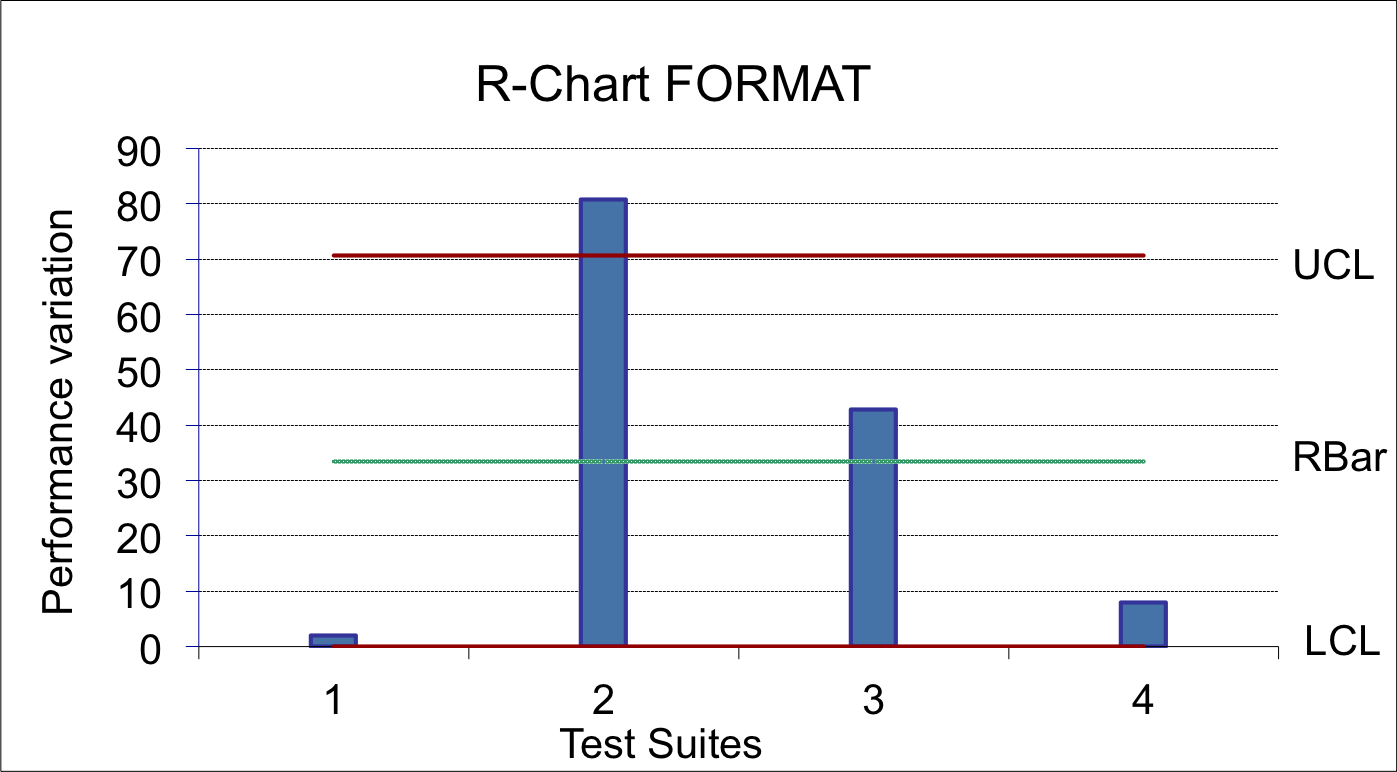
\includegraphics[width=0.48\linewidth]{chapitre4/fig/4.png}\label{rt4}}
	\subfigure[R-chart of the Promise benchmark program]{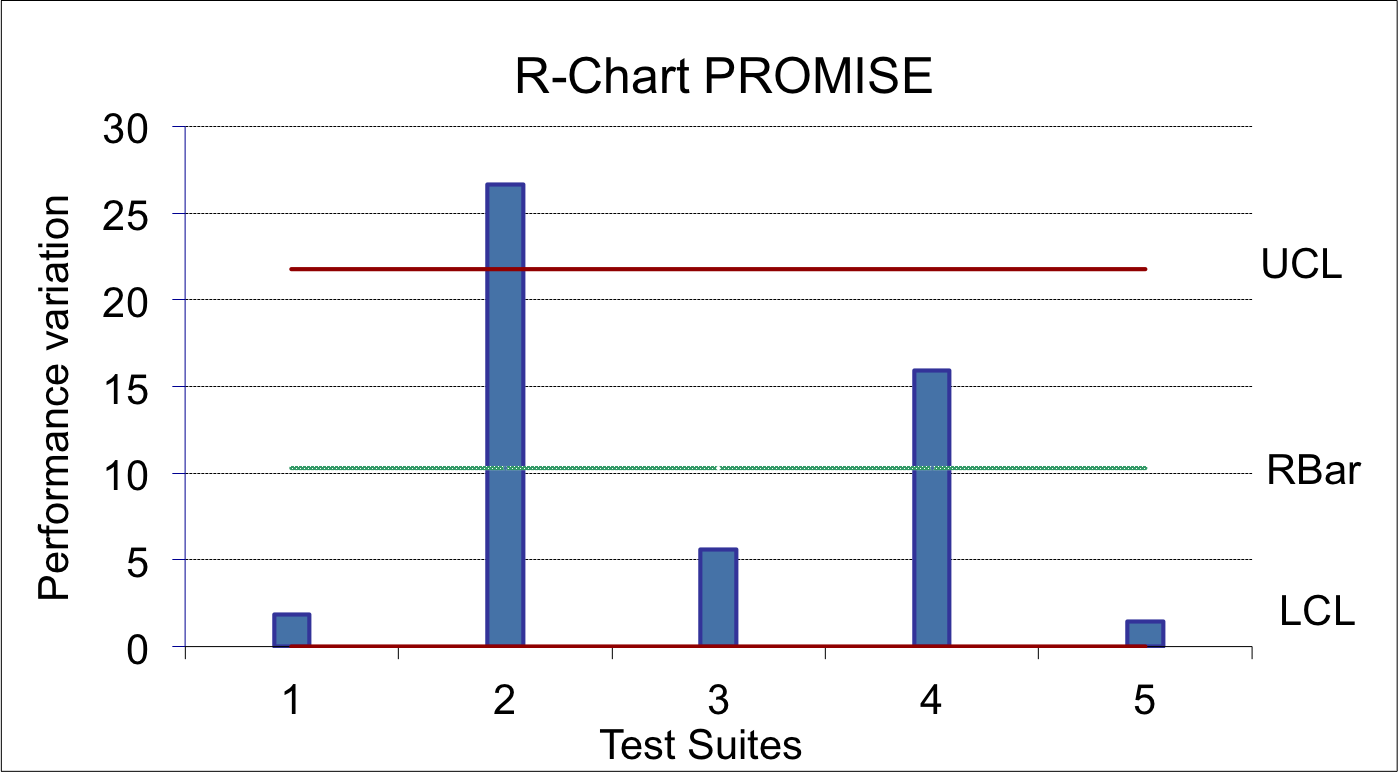
\includegraphics[width=0.48\linewidth]{chapitre4/fig/5.png}\label{rt5}}
	\subfigure[R-chart of the Culture benchmark program]{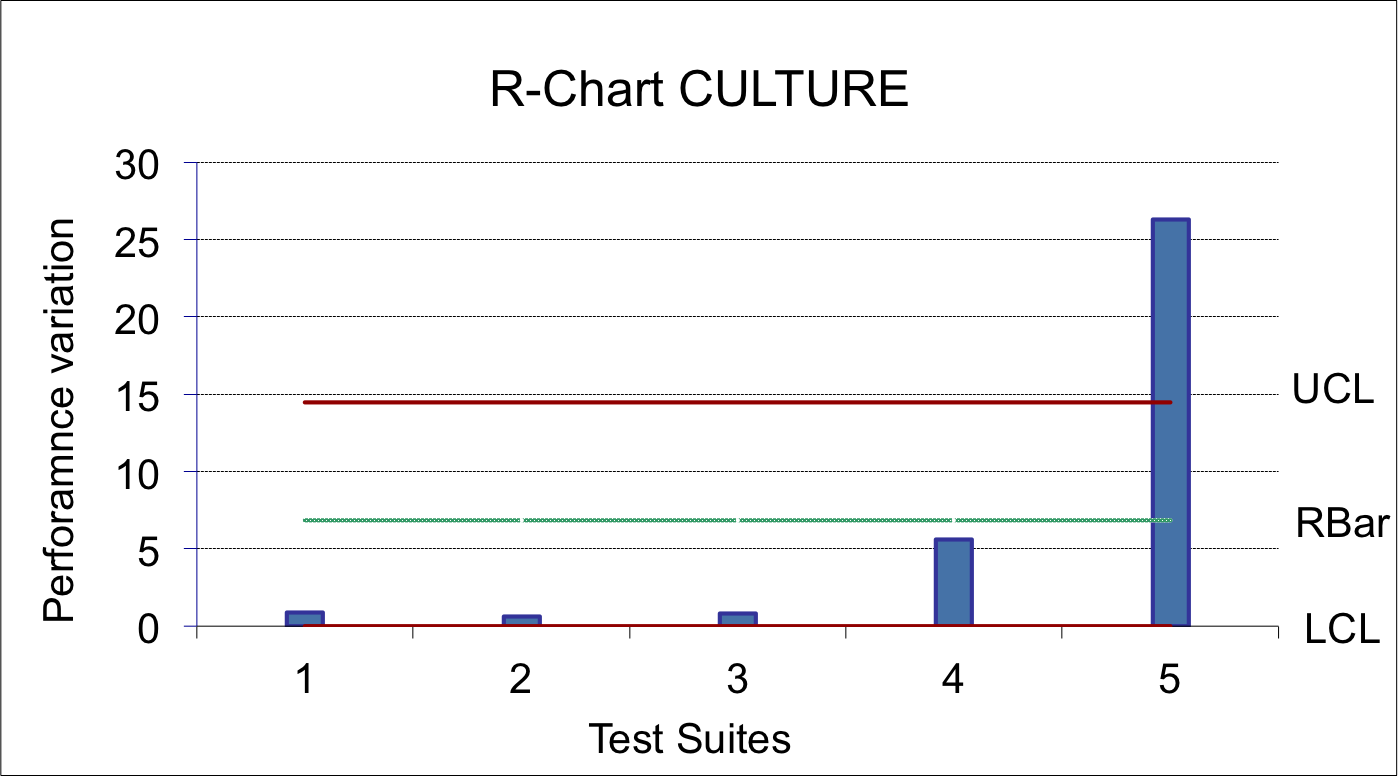
\includegraphics[width=0.48\linewidth]{chapitre4/fig/6.png}\label{rt6}}
	\subfigure[R-chart of the Math benchmark program]{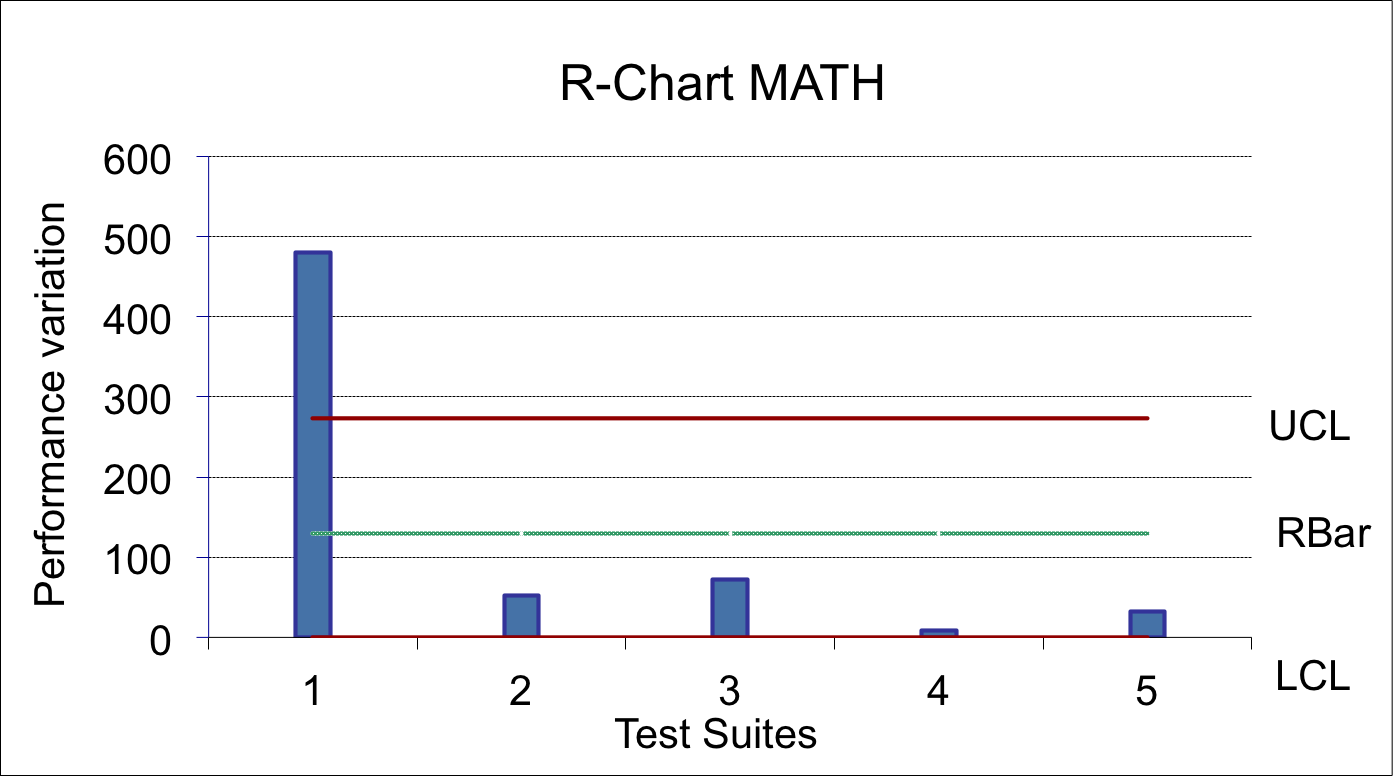
\includegraphics[width=0.48\linewidth]{chapitre4/fig/7.png}\label{rt7}}
	\caption{Performance variation of test suites across the different Haxe benchmarks}
	\label{rt}
\end{figure}

\begin{figure}
	\centering  
	\subfigure[R-chart of the Core benchmark program]{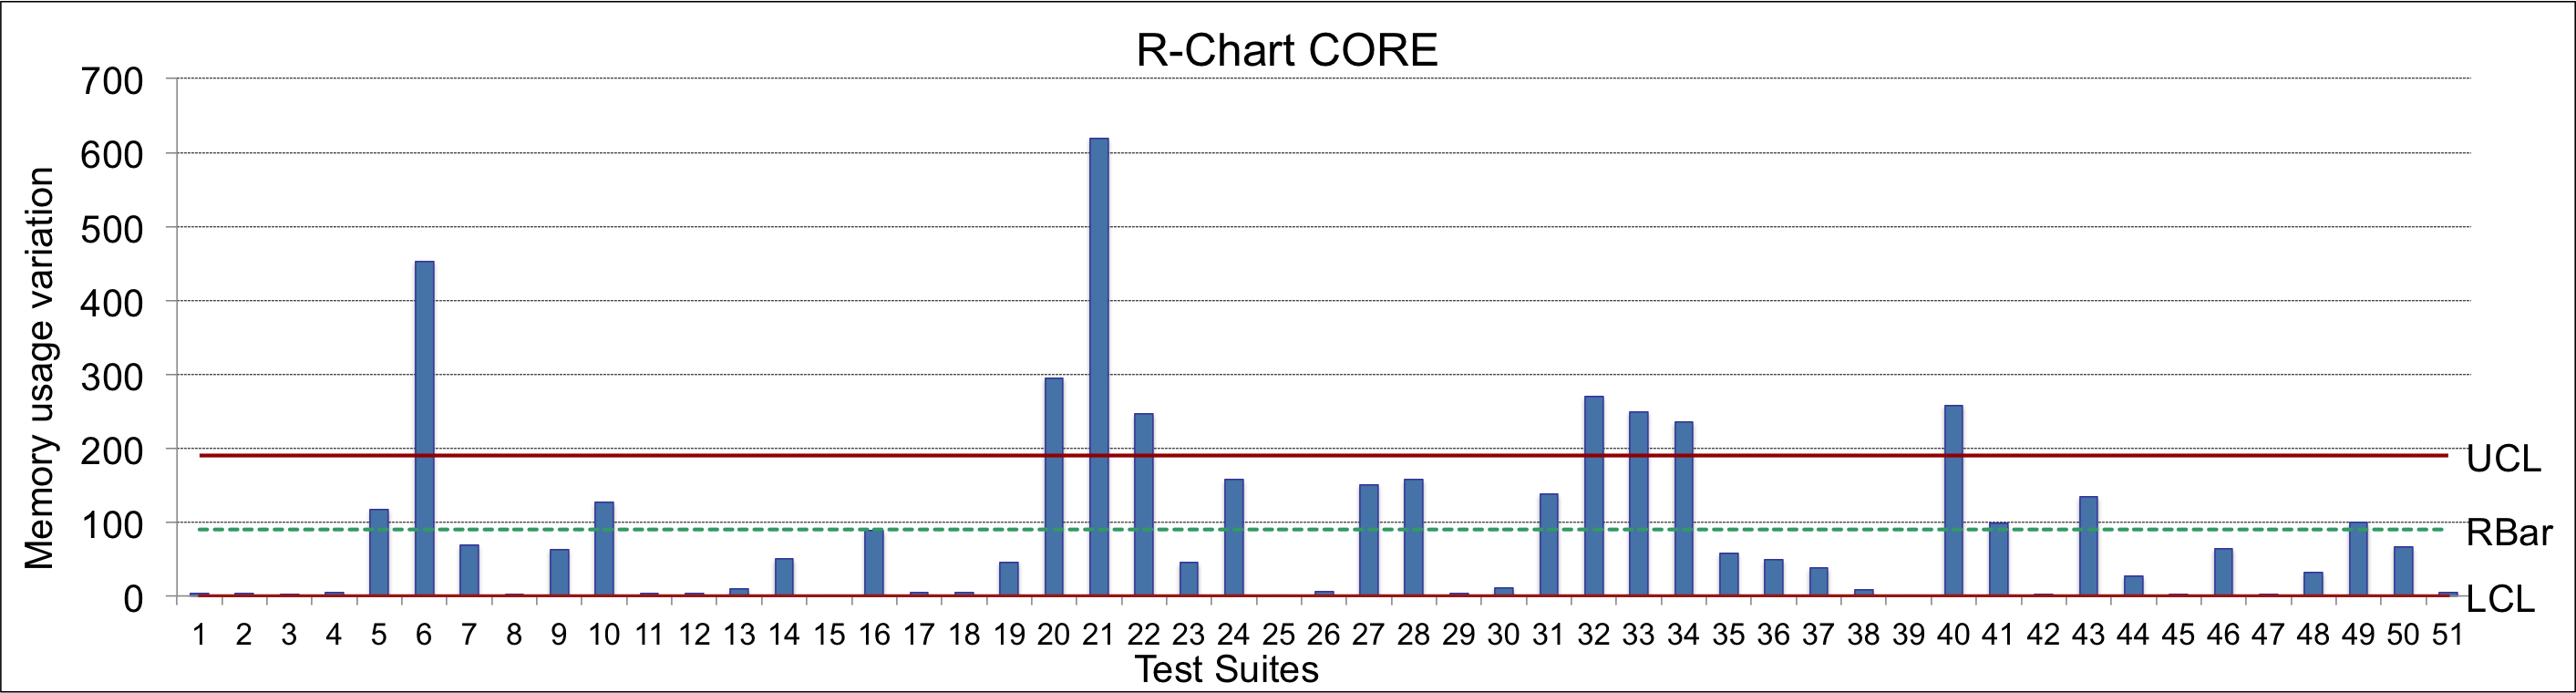
\includegraphics[width=0.96\linewidth]{chapitre4/fig/11.png}\label{rm1}}
	\subfigure[R-chart of the Color benchmark program]{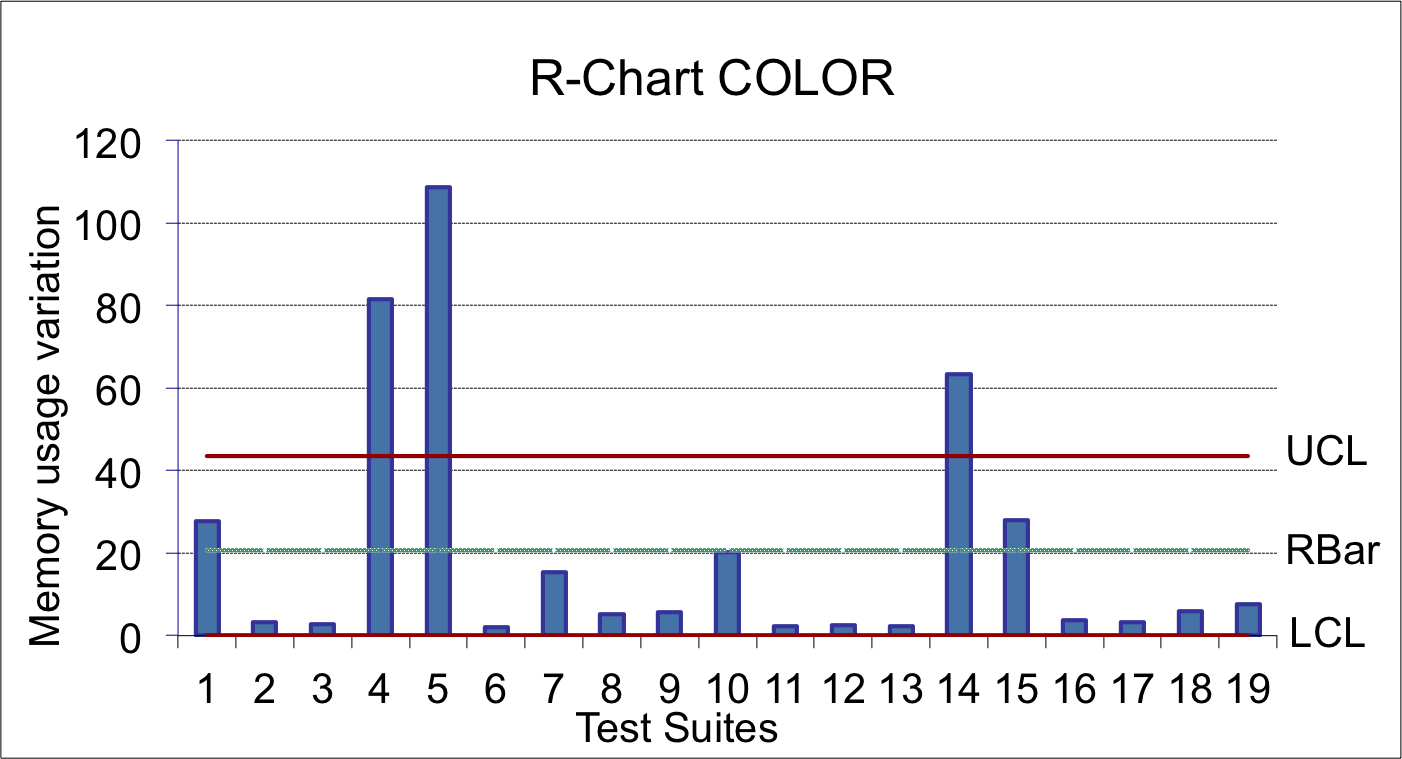
\includegraphics[width=0.48\linewidth]{chapitre4/fig/22.png}\label{rm2}}
	\subfigure[R-chart of the Hxmath benchmark program]{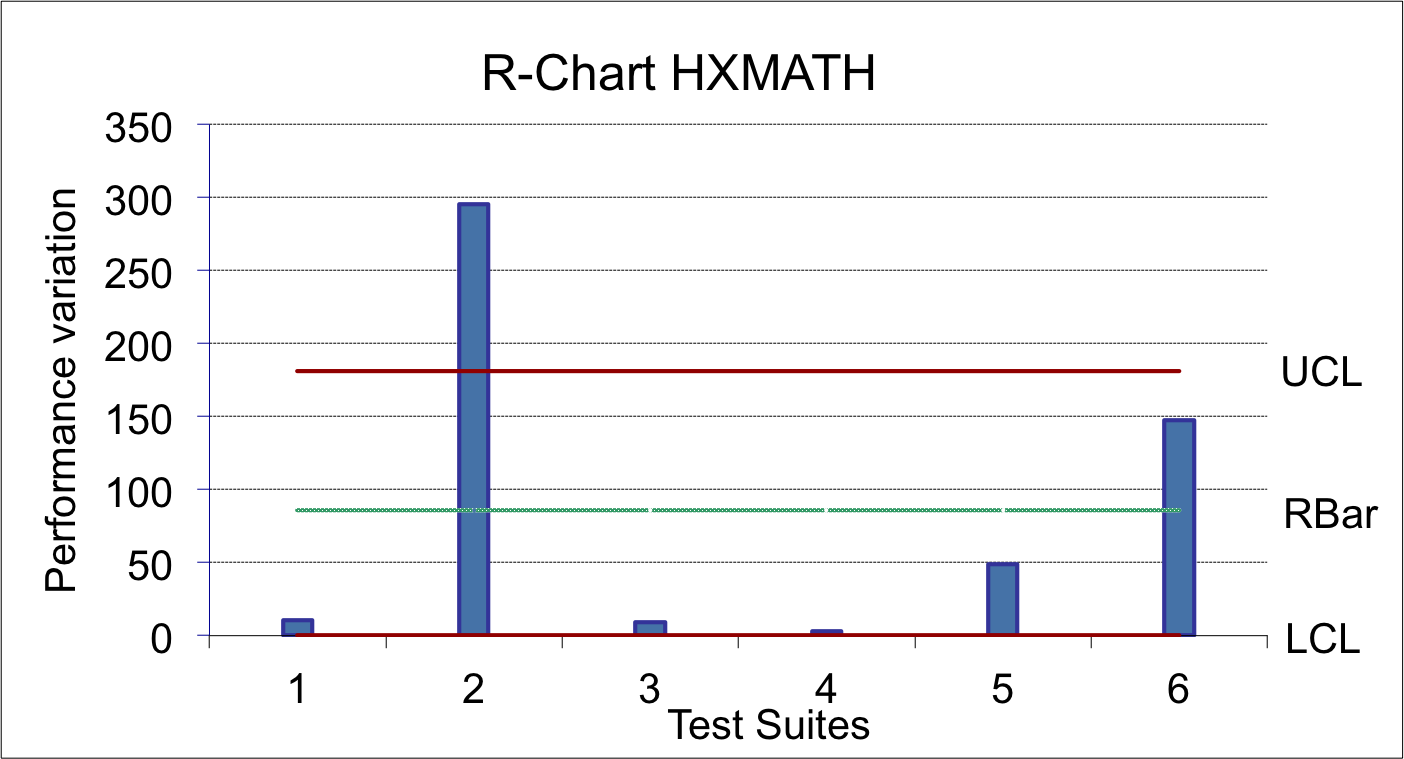
\includegraphics[width=0.48\linewidth]{chapitre4/fig/33.png}\label{rm3}}
	\subfigure[R-chart of the Format benchmark program]{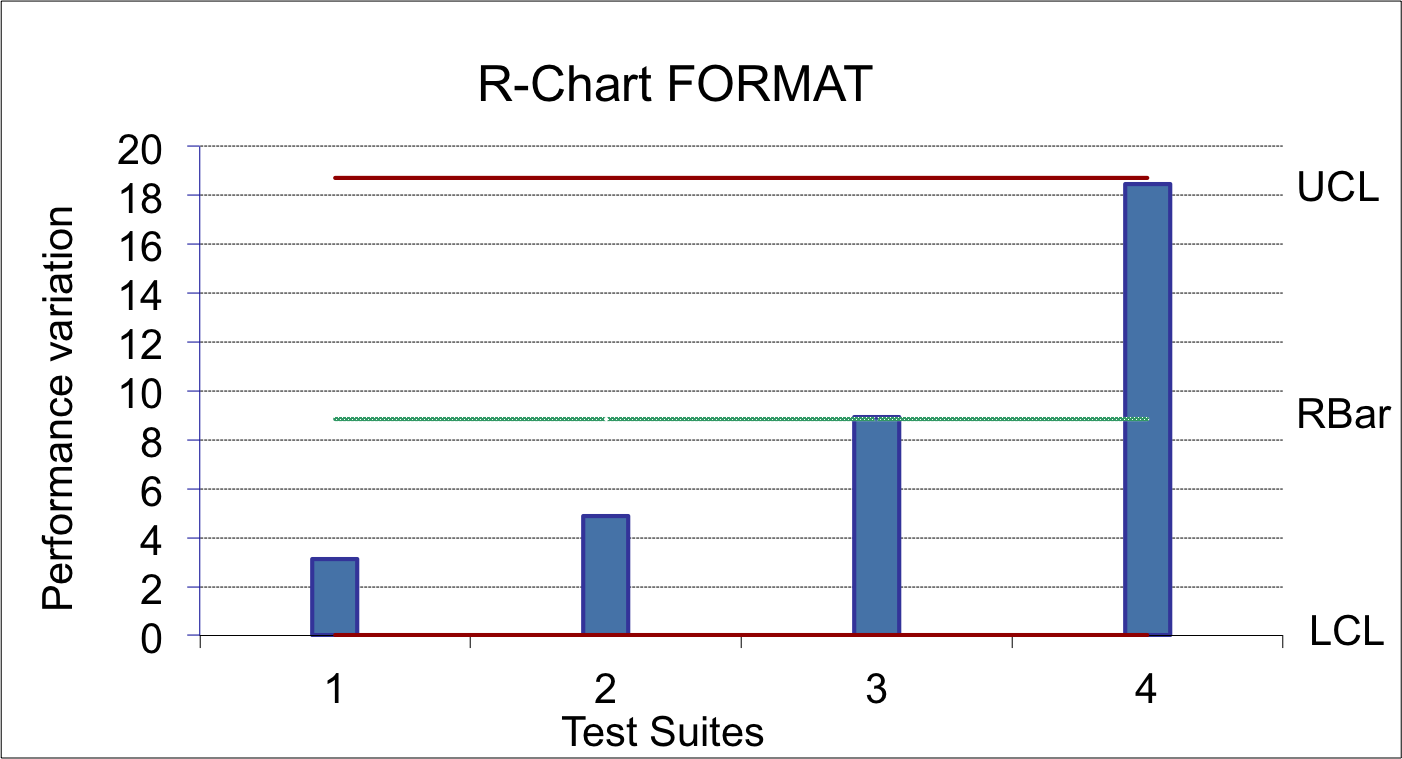
\includegraphics[width=0.48\linewidth]{chapitre4/fig/44.png}\label{rm4}}
	\subfigure[R-chart of the Promise benchmark program]{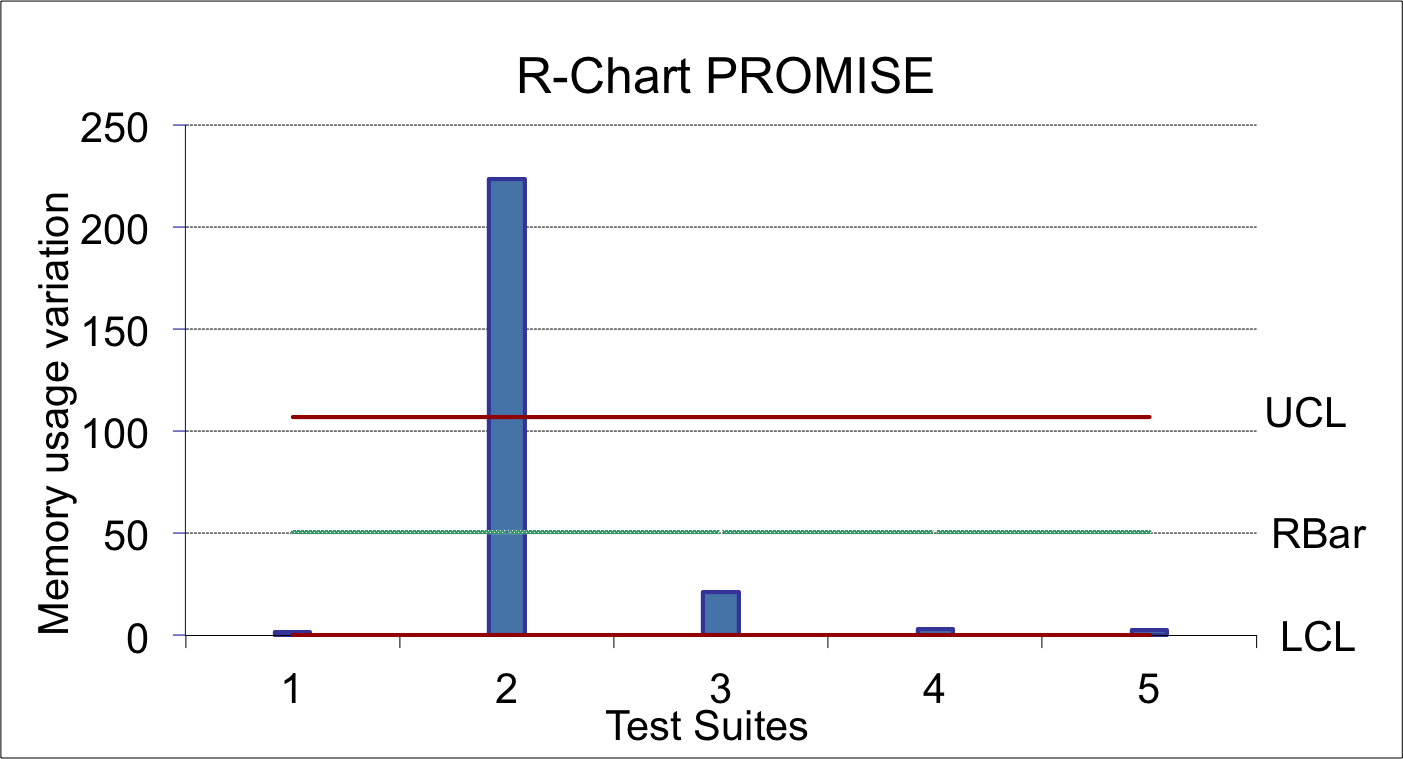
\includegraphics[width=0.48\linewidth]{chapitre4/fig/55.png}\label{rm5}}
	\subfigure[R-chart of the Culture benchmark program]{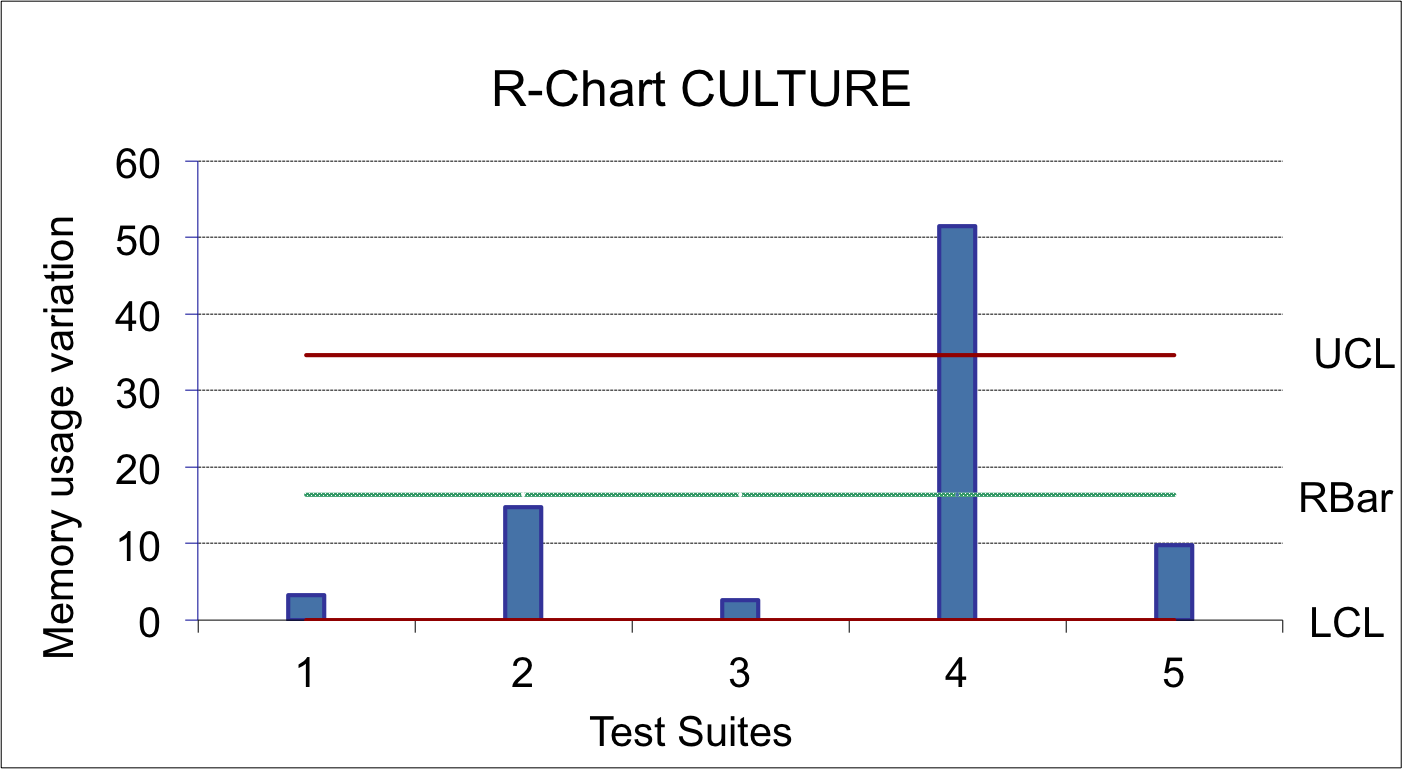
\includegraphics[width=0.48\linewidth]{chapitre4/fig/66.png}\label{rm6}}
	\subfigure[R-chart of the Math benchmark program]{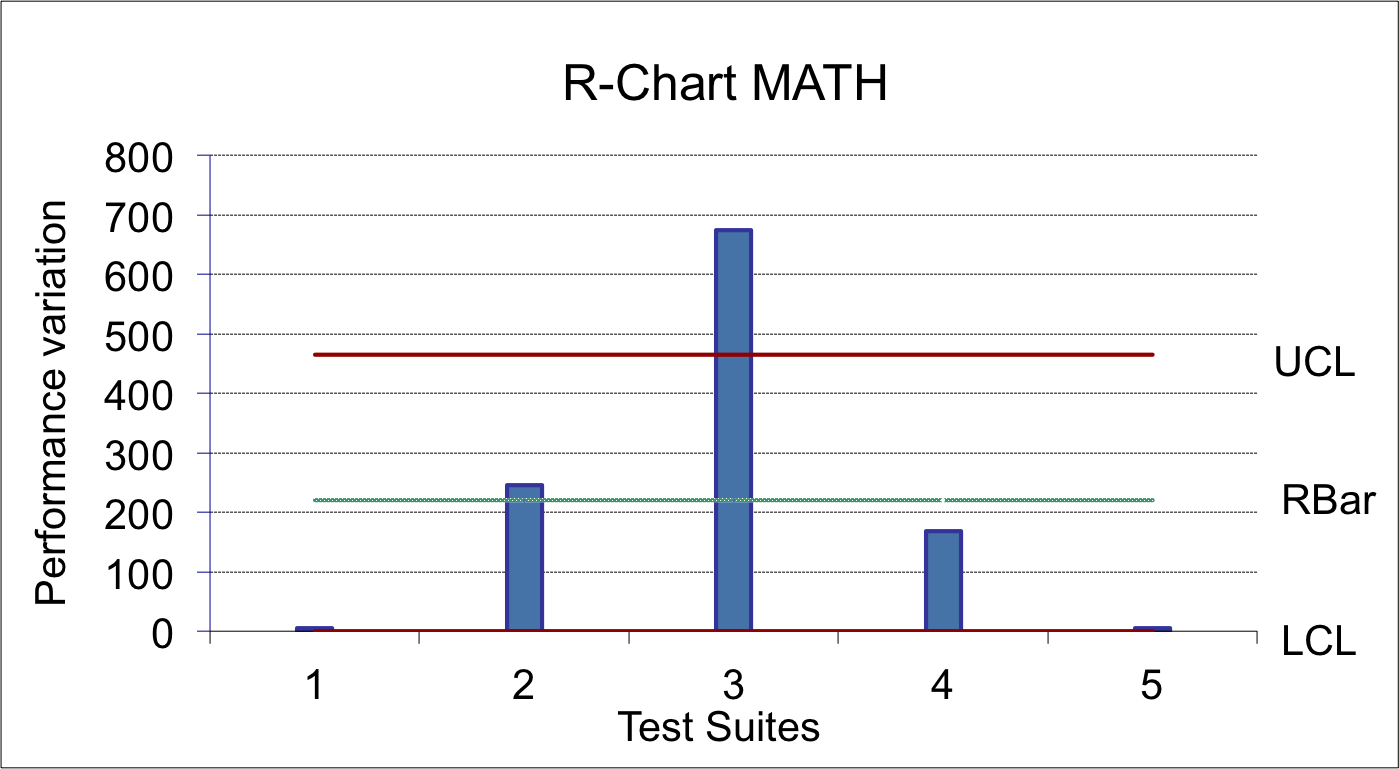
\includegraphics[width=0.48\linewidth]{chapitre4/fig/77.png}\label{rm7}}
	\caption{Memory usage variation of test suites across the different Haxe benchmarks}
	\label{rm}
\end{figure}
The results of R-charts for the seven benchmark programs relative to the performance and resource usage variations are reported in Figures \ref{rt} and \ref{rm}. In Figure \ref{rt}, we report the performance variation corresponding to the range difference $R$ between the maximum and minimum execution time of each test suite across the five targets (Java, JS, C++, C\#, and PHP). 
Data is normalized, dividing all values by the minimum execution time per test suite. 
The LCL for our experiments is always equal to 0 because the $D_{3}$ constant value as defined in equation \ref{eqUCL}, is equal to zero according to the R-chart constants table\footnote{\url{http://www.bessegato.com.br/UFJF/resources/table_of_control_chart_constants_old.pdf}}. In fact, the $D_{3}$ constant changes depending on the number of subgroups. In our experiments, our data record is composed of five subgroups corresponding to the five target programming languages.
The central line (in green) corresponds to $R$-$bar$. This value changes from one benchmark to another depending on the average of $R$ for all test suites in the benchmark. As a consequence, $UCL$, which is a function of $R$-$bar$, changes as long as we add new test suites to the experiments. $UCL$ is equal to $D_{4}*\bar{R}$ where $D_{4}=2.114$ according to the R-chart constants table. We recall that the average variation $R$-$bar$ and the threshold value $UCL$ change dynamically by adding new test suites to the corresponding benchmark. 
We note as well that these parameter values are appropriate to each benchmark program. We made the threshold values specific for each benchmark because we believe that the variation is highly dependent on the application domain and on the program under test. The R-charts used for visualizing the memory usage variation follow the same concept as we have just been describing for performance variation.  

Results in Figure \ref{rt}, show that most of the performance variations are in the interval $[0-UCL]$, which corresponds to \textit{in-control} variation zone as it is described in Section \ref{sec:cg-Variation threshold}. However, we remark for several test suites that the performance variation becomes relatively high (higher than the $UCL$ value of the corresponding benchmark program). We detect 11 among 95 performance deviations lying in the \textit{out of control} variation zone. For the other test suites, the variation is even less than the total average variations $R$-$bar$. There are only 7 test suites among the remaining 84 ones where the variation lies in the interval $[\bar{R}-UCL]$. This variation is high but we are not detecting it as a performance deviation because according to the R-chart, variation in this zone is still \textit{in-control}. 
The 11 performance deviations we have detected can be explained by the fact that the execution time of one or more test suites varies considerably from one language to another. This argues the idea that the code generator has produced a suspect code behavior, which led to a high performance variation. We provide later better explanation about the faulty code generators.

Similarly, Figure \ref{rm} resumes the comparison results of test suites execution regarding the memory usage. The variation in this experiment are more important than previous results. This can be argued by the fact that the memory utilization and allocation patterns are different from one language to another. Nevertheless, we can recognize some points where the variation is extremely high. Thus, we detect 15 among 95 test suites that exceed the corresponding $UCL$ value. 
When the variation is below UCL, we detect 14 among the 80 remaining test suites where the variation lies in the interval $[\bar{R}-UCL]$, which is relatively high. 
One of the reasons that caused this variation may occur when the test suite executes some parts of the code (in a specific language) that strangely consume a lot of resources. This may not be the case when the variation is lower than the $\bar{R}$ for example.


To resume, we have detected 11 extreme performance variations and 15 extreme memory usage variations among the 95 executed test suites. We assume then, that faulty code generators, in identified points, represent a threat for software quality since the generated code has shown symptoms of poor-quality design. 



\paragraph{PCA results}~\\
\begin{figure}
	\centering  
	\subfigure[Test suites relative to the execution times ]{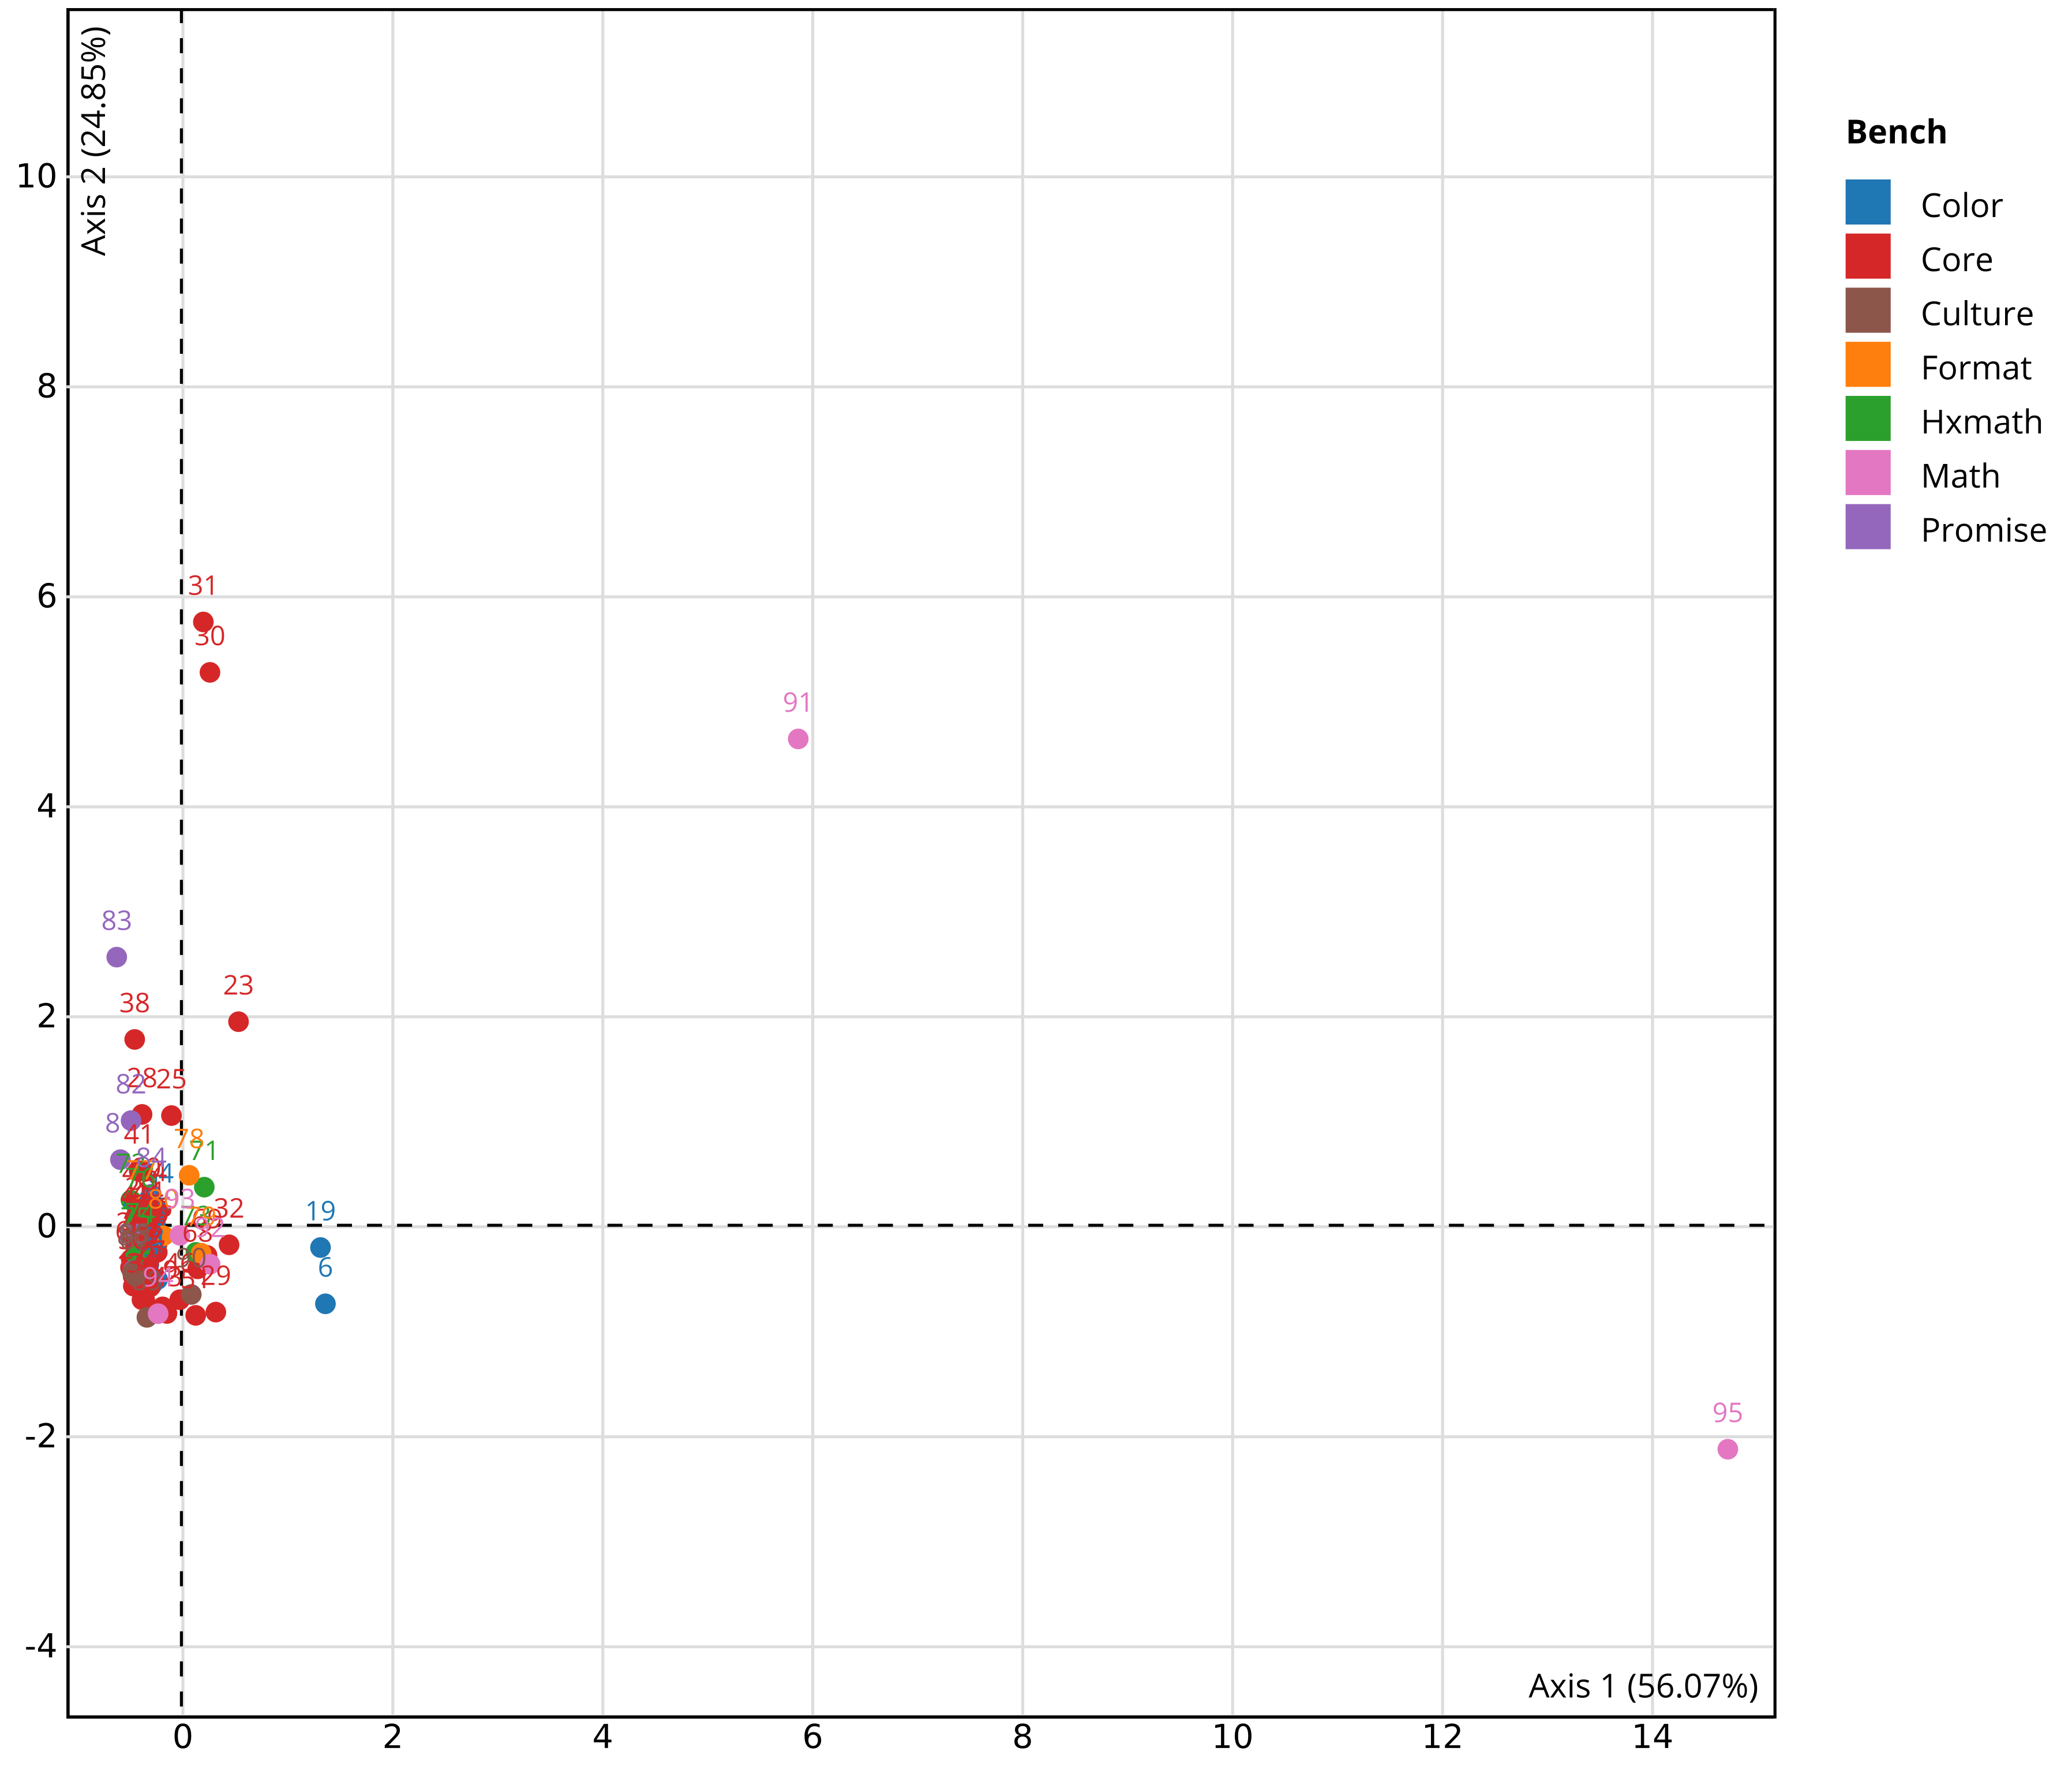
\includegraphics[width=0.7\linewidth]{chapitre4/fig/explor_ind}\label{pcat}}
	\subfigure[Test suites relative to the memory consumptions]{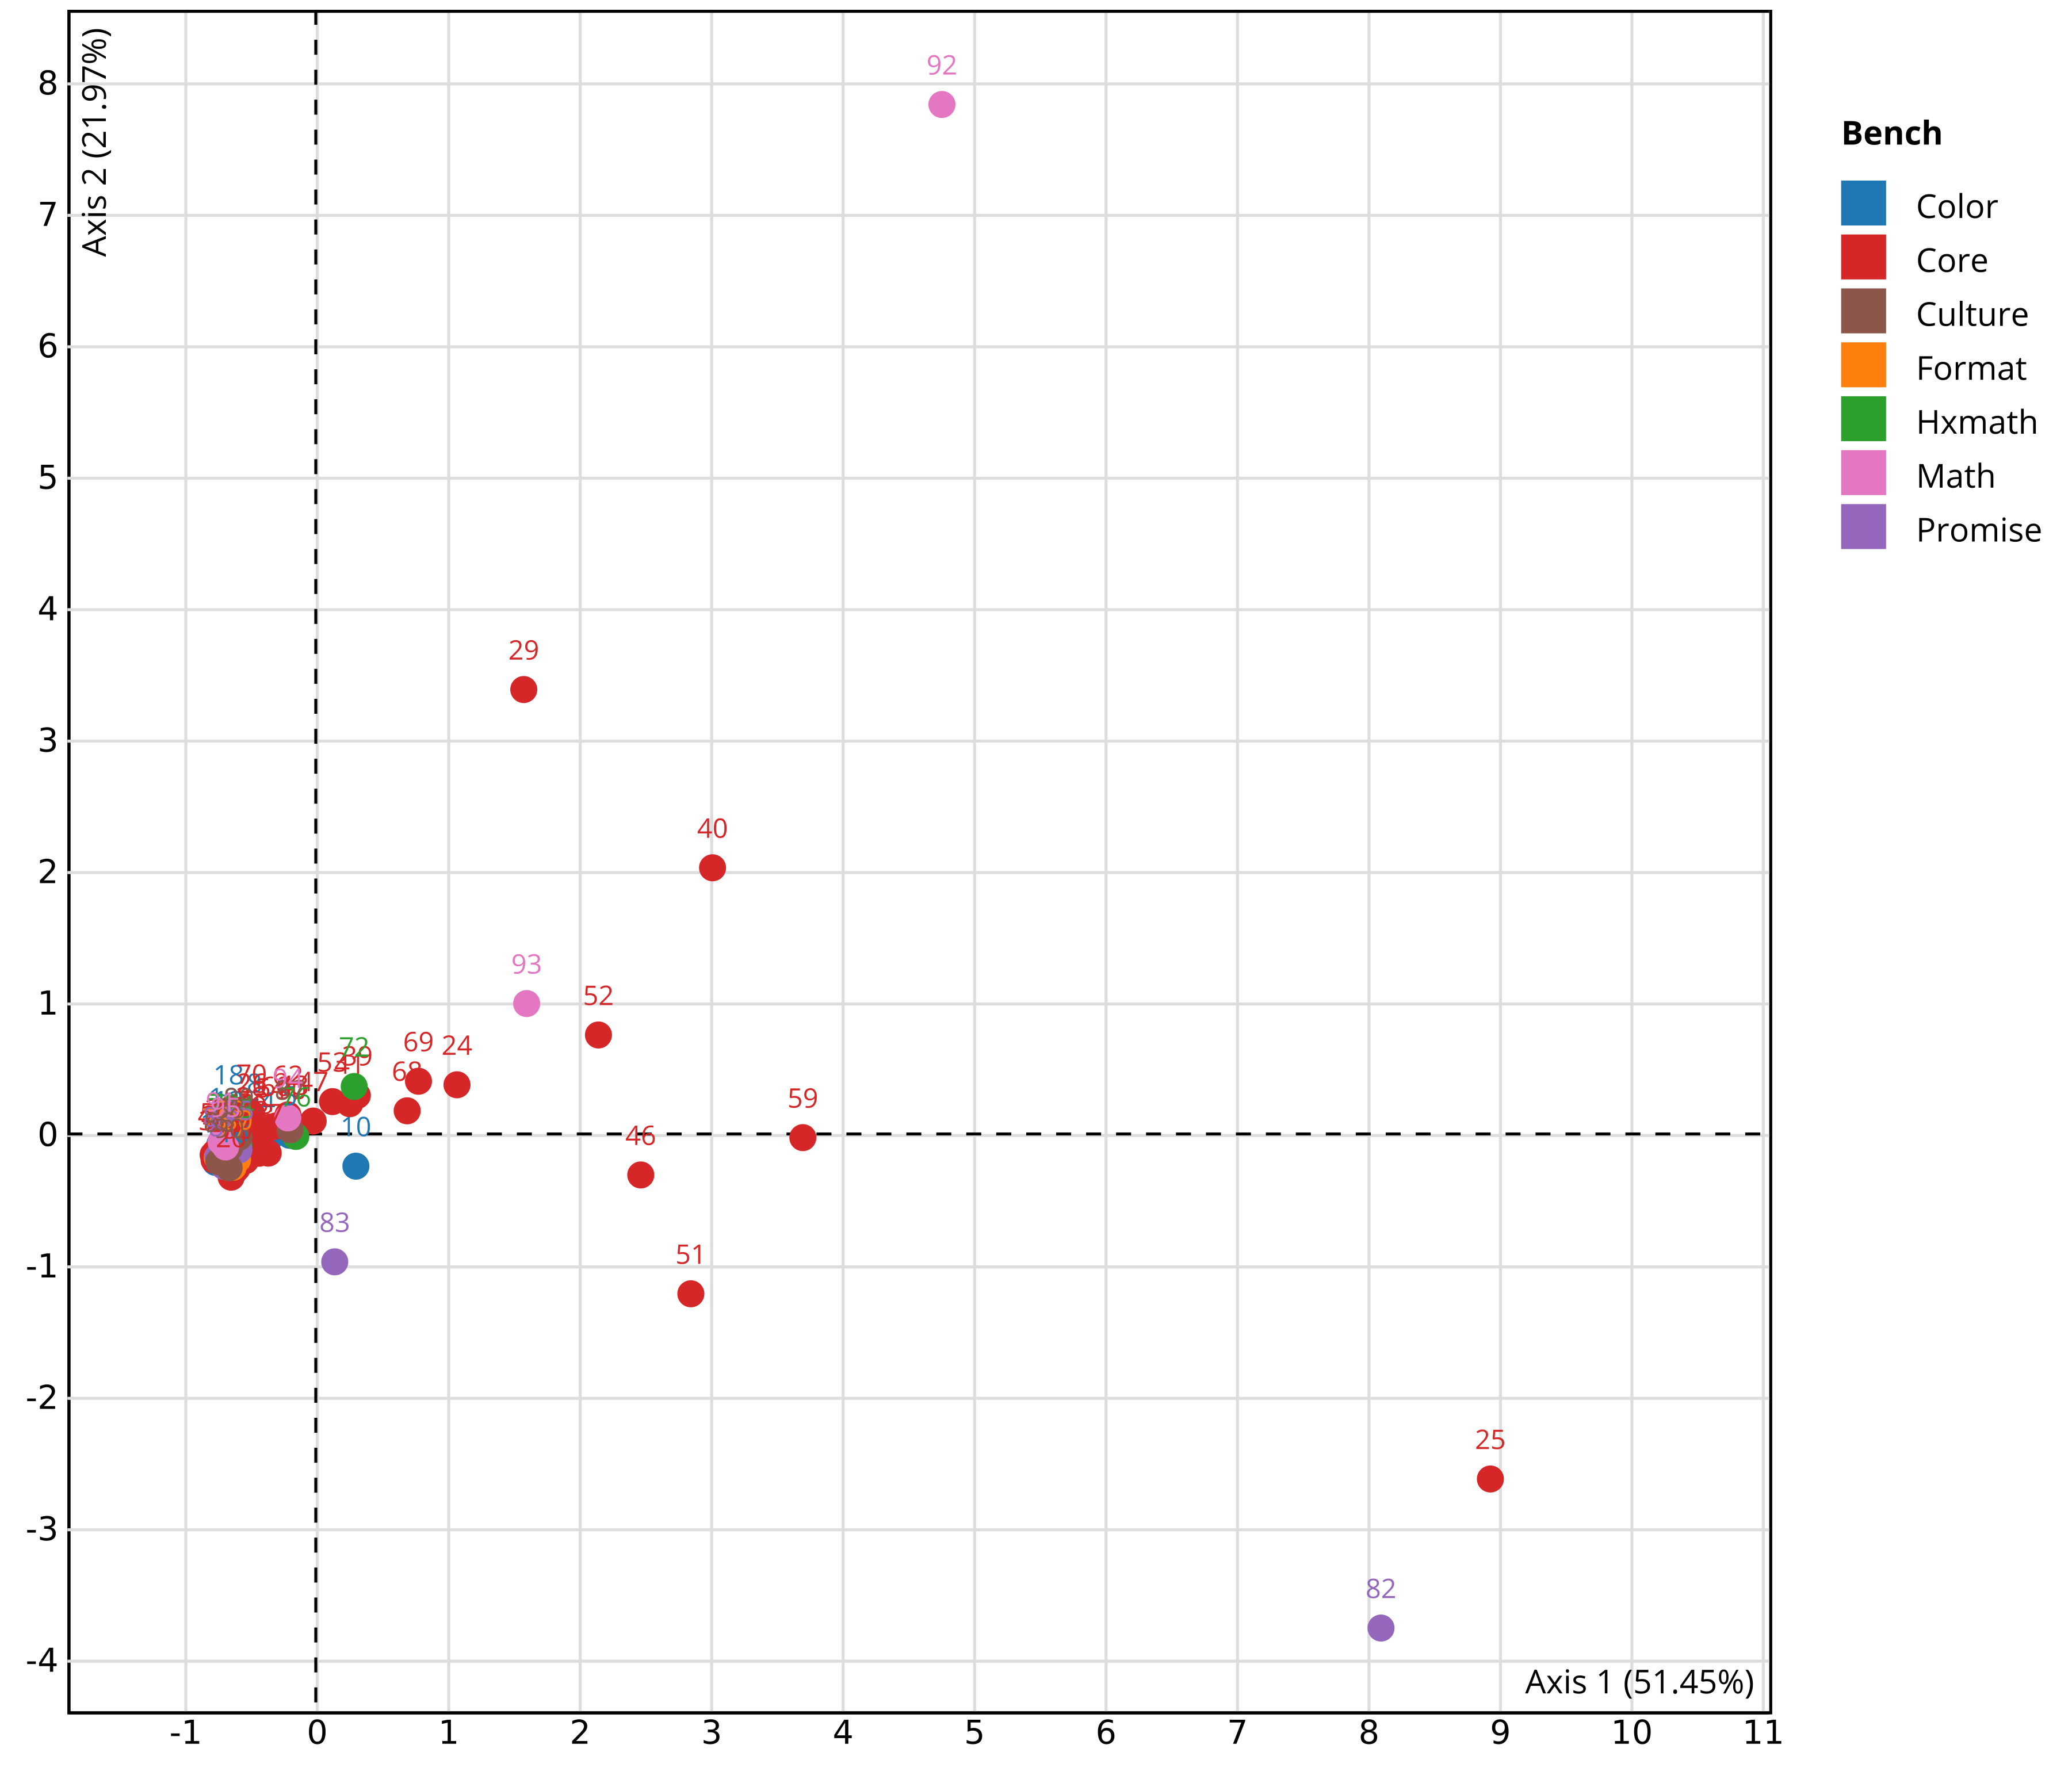
\includegraphics[width=0.7\linewidth]{chapitre4/fig/explor_ind2}\label{pcam}}
	\caption{PCAs showing the dispersion of our data over the PC subspace}
	\label{pca}
\end{figure}
\begin{figure}
	\centering  
	\subfigure[Performance deviations]{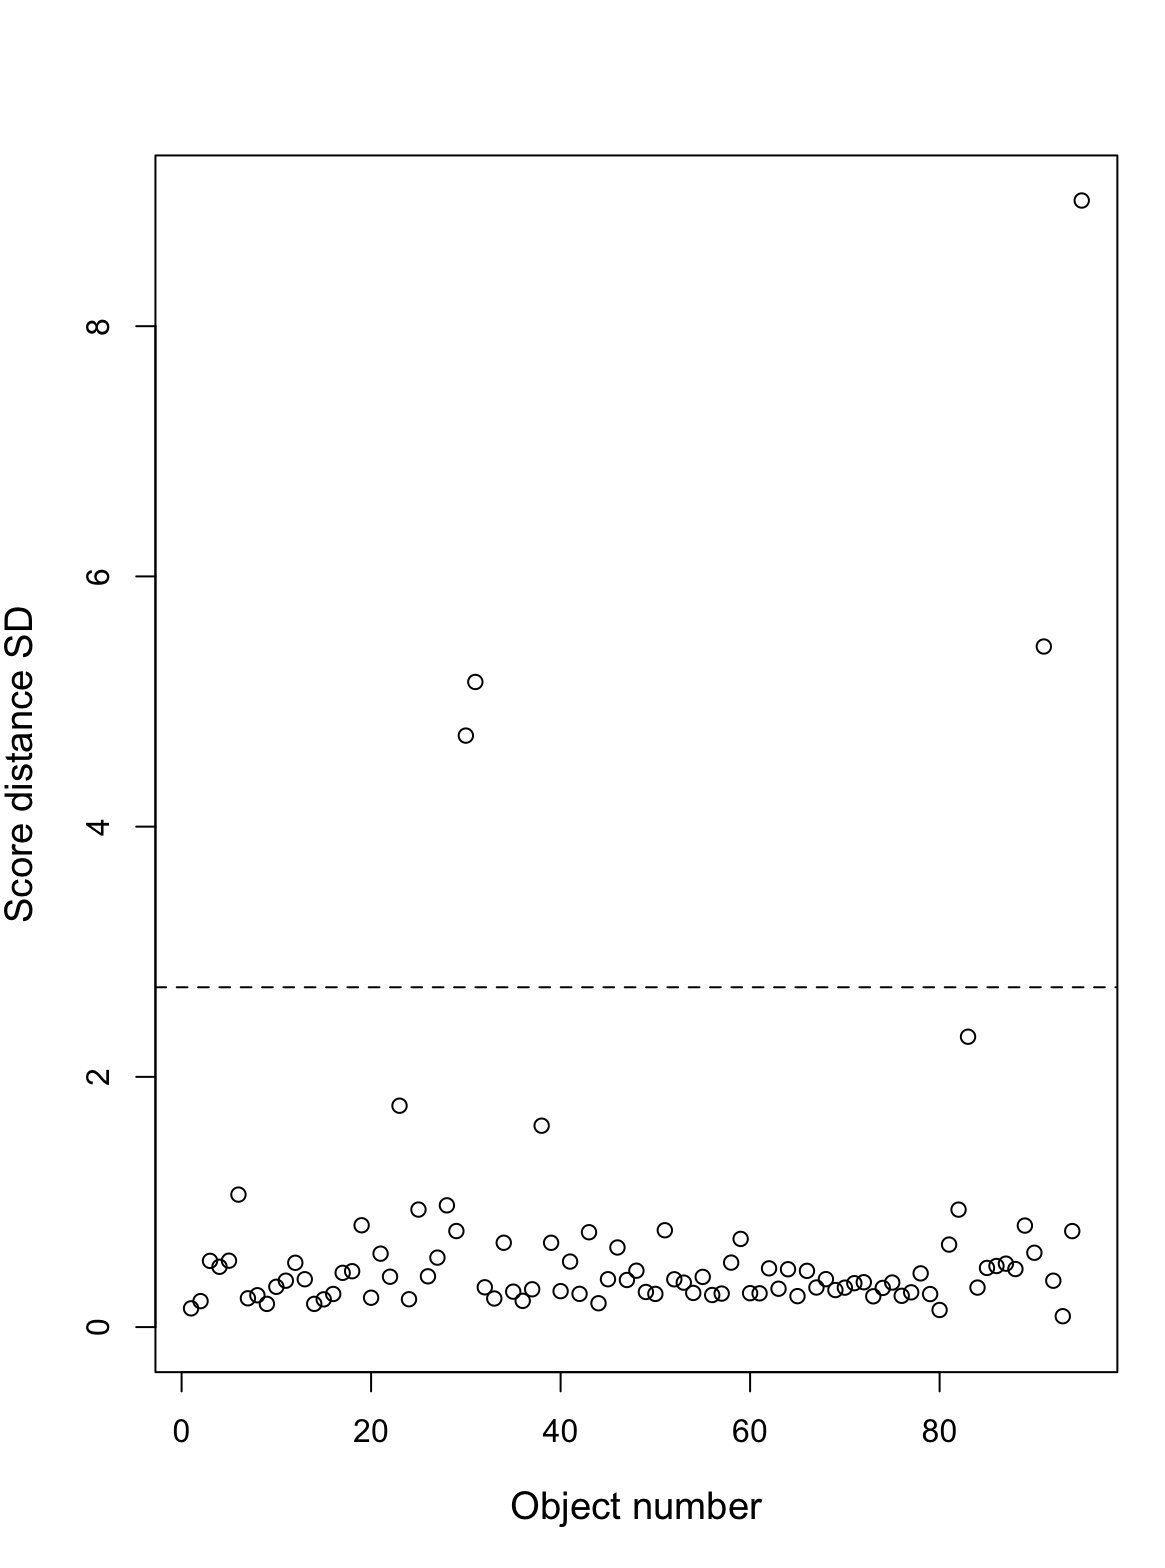
\includegraphics[width=0.49\linewidth]{chapitre4/fig/mahatime}\label{sdt}}
	\subfigure[Memory usage deviations]{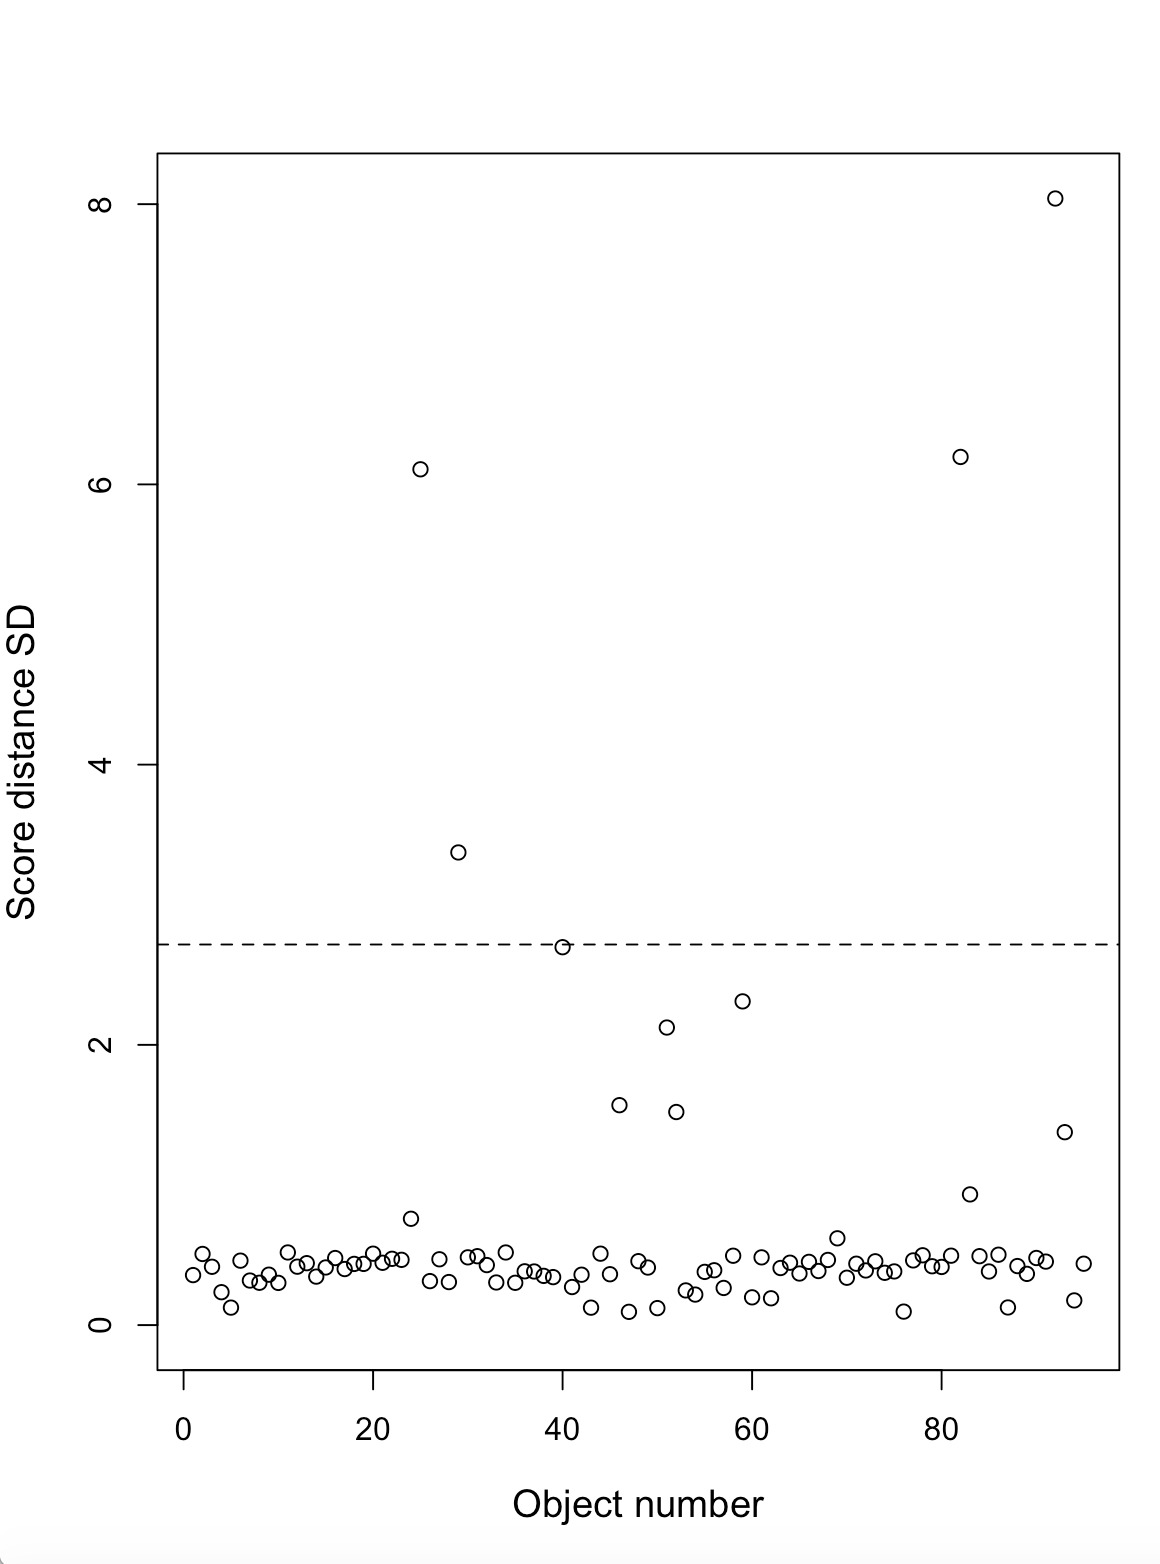
\includegraphics[width=0.49\linewidth]{chapitre4/fig/mahamem}\label{sdm}}
	
	\caption{Diagnostic plots using score distance SD. The vertical lines indicate critical values separating regular observations from outliers (97.5\%)}
	\label{sd}
\end{figure}
We apply the PCA approach as an alternative to the R-chart approach. Figure \ref{pca} shows the dispersion of our data points in the PC subspace. PC1 et PC2 represent the directions of our two first principal components, having the highest orthogonal variations. Our data points represent the performance variation (Figure \ref{pcat}) and the memory usage variation (Figure \ref{pcam}) of the 95 test suites we have executed. Variation points are colored according to the benchmark program they belong to (displayed in the figure legend). At the first glance, we can clearly see that the variation points are situated in the same area except some points that lie far from this data cluster. In Figure \ref{pcat}, the pink points corresponding to the Math benchmark show visually the largest variation. The three Core test suites (in red) which are identified as performance deviations in R-chat, show also a deviation in the PCA scatter plot. Points 91 relative to the Math benchmark is deviating from the cloud point. However, in the R-chart diagram, it is not detected as a performance deviation (see the test suite 3 of Figure \ref{rt7}). In fact, this test suite takes more than 80 times to run. Compared to other test suites, the performance variation does not exceed 80. In effect, PCA performs a complete analysis of the whole data we have collected in all benchmarks. Thus, variations are displayed with respect to all test suites variations in all benchmarks. The variation evaluation is not limited within the benchmark program as we used to do using R-charts. We report the same results in Figure \ref{pcam} about the memory usage variation in the PCA. 


To confirm this observation, we present in Figure \ref{sd}, the results of our outliers detection approach. We identify 4 inconsistencies (or outliers) in each diagnostic plot. Inconsistencies in Figure \ref{pcat} are relative to the performance deviations. Points 31 and 32 correspond to the test suites 12 and 11 in benchmark Core of Figure \ref{rt1}. Points 91 and 95 correspond to the test suites 3 and 1 in benchmark Math of Figure \ref{rt7}. For memory usage variation, we detect points 25, 29, 82, and 92 which corresponds relatively to the test suites 21 and 6 of benchmark Core, 2 of benchmark Promise, and 3 of benchmark Math.
We can clearly see that this technique helps to identify extreme-value outliers, which are mostly covered by the R-chart approach. We used 97.5\%-Quantile of the Chi-square distribution to define the cutoff value which is commonly used in the literature\cite{enot2008preprocessing,hubert2009robust}. If we decrease this value we will be able to detect more variation points. 


\paragraph{Detected inconsistencies }~\\
\begin{table*}[h]
	\centering
	
	\resizebox{\columnwidth}{!}{%
		\begin{tabular}{|c|c|c|c|c|c|c|c|c|}
			\hline
			\textbf{Benchamrk}                & \textbf{Test Suite}            & \textbf{Java} & \textbf{JS} & \textbf{CPP} & \textbf{CS} & \textbf{PHP}                   & \textbf{UCL(R)}         & \textbf{Defective CG} \\ \hline
			\textbf{Color}                    & \textbf{TS19}                  & 1.90          & 1           & 2.37         & 3.31        & \cellcolor[HTML]{E3E3E3}61.84  & 13.08                   & PHP                   \\ \hline
			&                                & 1             & 1.59        & 1.67         & 2.78        & \cellcolor[HTML]{E3E3E3}148.20 &                         & PHP                   \\ \cline{3-7} \cline{9-9} 
			&                                & 1.14          & 2.71        & 1            & 3.63        & \cellcolor[HTML]{E3E3E3}258.94 &                         & PHP                   \\ \cline{3-7} \cline{9-9} 
			&                                & 1.28          & 2.94        & 1            & 3.36        & \cellcolor[HTML]{E3E3E3}261.36 &                         & PHP                   \\ \cline{3-7} \cline{9-9} 
			\multirow{-4}{*}{\textbf{Core}}   & \multirow{-4}{*}{\textbf{TS4}} & 1             & 1.05        & 1.86         & 2.39        & \cellcolor[HTML]{E3E3E3}50.30  & \multirow{-4}{*}{43.62} & PHP                   \\ \hline
			&                                & 2.38          & 1.43        & 1            & 2.82        & \cellcolor[HTML]{E3E3E3}51.72  &                         & PHP                   \\ \cline{3-7} \cline{9-9} 
			\multirow{-2}{*}{\textbf{Hxmath}} & \multirow{-2}{*}{\textbf{TS1}} & 2.14          & 1.10        & 1            & 2.25        & \cellcolor[HTML]{E3E3E3}50.56  & \multirow{-2}{*}{42.97} & PHP                   \\ \hline
			\textbf{Format}                   & \textbf{TS2}                   & 1.16          & 1.27        & 1            & 3.35        & \cellcolor[HTML]{E3E3E3}81.85  & 70.66                   & PHP                   \\ \hline
			\textbf{Promise}                  & \textbf{TS2}                   & 1.52          & 1.85        & 1            & 1.51        & \cellcolor[HTML]{E3E3E3}27.67  & 21.76                   & PHP                   \\ \hline
			\textbf{Culture}                  & \textbf{TS5}                   & 1.62          & 1           & 1.27         & 2.02        & \cellcolor[HTML]{E3E3E3}27.29  & 14.47                   & PHP                   \\ \hline
			\textbf{Math}                     & \textbf{TS1}                   & 4.15          & 1           & 5.41         & 4.70        & \cellcolor[HTML]{E3E3E3}481.68 & 273.24                  & PHP                   \\ \hline
		\end{tabular}%
	}
	\caption{Raw data values of test suites that led to the highest variation in terms of execution time}
	\label{perf-tab}`
\end{table*}

\begin{table*}[h]
	\centering
	
	\resizebox{\columnwidth}{!}{%
		\begin{tabular}{|c|c|c|c|c|c|c|c|c|}
			\hline
			\textbf{Benchmark}               & \textbf{Test suite} & \textbf{Java}                  & \textbf{JS} & \textbf{CPP} & \textbf{CS} & \cellcolor[HTML]{FFFFFF}\textbf{PHP} & \textbf{UCL}             & \textbf{Defective CG} \\ \hline
			& \textbf{TS4}        & 1                              & 2.29        & 1.47         & 3.59        & \cellcolor[HTML]{E8E8E8}82.46        &                          & PHP                   \\ \cline{2-7} \cline{9-9} 
			& \textbf{TS5}        & 1                              & 3.08        & 1.83         & 4.53        & \cellcolor[HTML]{E8E8E8}109.69       &                          & PHP                   \\ \cline{2-7} \cline{9-9} 
			\multirow{-3}{*}{\textbf{Color}} & \textbf{TS14}       & 1                              & 1.32        & 1.00         & 2.03        & \cellcolor[HTML]{E8E8E8}64.45        & \multirow{-3}{*}{43.53}  & PHP                   \\ \hline
			& \textbf{TS6}        & \cellcolor[HTML]{E8E8E8}250.77 & 71.71       & 1            & 69.90       & \cellcolor[HTML]{E8E8E8}454.15       &                          & PHP \& Java           \\ \cline{2-7} \cline{9-9} 
			& \textbf{TS20}       & 2.31                           & 1.34        & 1            & 3.27        & \cellcolor[HTML]{E8E8E8}296.10       &                          & PHP                   \\ \cline{2-7} \cline{9-9} 
			& \textbf{TS21}       & 11.90                          & 1           & 14.63        & 36.18       & \cellcolor[HTML]{E8E8E8}620.22       &                          & PHP                   \\ \cline{2-7} \cline{9-9} 
			& \textbf{TS22}       & 1                              & 2.70        & 1.74         & 4.69        & \cellcolor[HTML]{E8E8E8}247.32       &                          & PHP                   \\ \cline{2-7} \cline{9-9} 
			& \textbf{TS32}       & \cellcolor[HTML]{E8E8E8}270.78 & 2.27        & 1            & 5.61        & 153.37                               &                          & Java                  \\ \cline{2-7} \cline{9-9} 
			& \textbf{TS33}       & 1.82                           & 1.12        & 1            & 54.19       & \cellcolor[HTML]{E8E8E8}250.35       &                          & PHP                   \\ \cline{2-7} \cline{9-9} 
			& \textbf{TS34}       & 1                              & 1.17        & 1.48         & 3.90        & \cellcolor[HTML]{E8E8E8}236.97       &                          & PHP                   \\ \cline{2-7} \cline{9-9} 
			\multirow{-8}{*}{\textbf{Core}}  & \textbf{TS40}       & 160.84                         & 1.10        & 1            & 49.43       & \cellcolor[HTML]{E8E8E8}259.20       & \multirow{-8}{*}{190.03} & PHP                   \\ \hline
			\textbf{Hxmath}                  & \textbf{TS2}        & 1                              & 1.16        & 1.91         & 2.82        & \cellcolor[HTML]{E8E8E8}296.16       & 181.11                   & PHP                   \\ \hline
			\textbf{Promise}                 & \textbf{TS2}        & \cellcolor[HTML]{E8E8E8}214.53 & 92.45       & 1            & 57.68       & \cellcolor[HTML]{E8E8E8}224.41       & 106.82                   & PHP \& Java           \\ \hline
			\textbf{Culture}                 & \textbf{TS4}        & 2.75                           & 1.01        & 2.52         & 1           & \cellcolor[HTML]{E8E8E8}52.47        & 34.63                    & PHP                   \\ \hline
			\textbf{Math}                    & \textbf{TS3}        & 1.29                           & 1           & 1.72         & 3.60        & \cellcolor[HTML]{E8E8E8}675.00       & 464.80                   & PHP                   \\ \hline
		\end{tabular}%
	}
	\caption{Raw data values of test suites that led to the highest variation in terms of memory usage}
	\label{mem-tab}`
\end{table*}

Now that we have observed the performance and memory usage variations of test suites execution, we can analyze the extreme points we have detected using R-chart to observe in greater depth the source of such deviation.
For that reason, we present in Table \ref{perf-tab} and \ref{mem-tab} the raw data values of these test suites leading to an extreme variation in terms of execution time and memory usage. We report the inconsistencies gathered from the first approach, R-chart.

Table \ref{perf-tab} shows the execution time factor of each test suite execution in a specific target language. This factor is scaled with respect to the the lowest execution time among the five targets. We also report the $UCL$ defined per benchmark. In the last column, we report the code generator that caused such large deviation. To do so, we designate by \textit{defective CG}, the code generator that led to a performance variation higher than the $UCL$ value.

We can clearly see that the PHP code has a singular behavior regarding the performance with a factor ranging from x27.29 for test suite 5 in benchmark Culture (Culture\_TS5) to x481.7 for Math\_TS1. For example, if Math\_TS1 takes $1$ minute to run in JS, the same test suite in PHP will take around $8$ hours to run which is a very large gap. 
The highest factor detected for other languages is x5.41 which is not negligible but it represents a small deviation compared to PHP deviations. While it is true that we are comparing different versions of generated code, it was expected to get some variations while running test cases in terms of execution time. However, in the case of PHP code generator, it is far to be a simple variation, but it is a code generator inconsistency that led to such performance regression.


Meanwhile, we gather information about the points that led to the highest variation in terms of memory usage. Table \ref{mem-tab} shows these results. 
Again, we can identify a singular behavior of the PHP code regarding the memory usage with a factor ranging from x52.47 to x675. For other test suites versions, the factor varies from x1 to x160.84. We observe as well a singular behavior of the Java code for Core\_TS6, Core\_TS32, and Promise\_TS2, yielding to a variation higher than the $UCL$. 
These results prove that the PHP and Java code generators are not always effective and they constitute a threat for the generated software in terms of memory usage.

%Besides the performance issues of PHP code generator presented in table~5, the results of memory usage confirm our claim since the PHP code has the highest memory utilization.

%The inconsistencies we found are more related to the incorrect memory utilization patterns produced by the defective code generator, or by generating a non-optimized and efficient code . Such inconsistencies may come from an inadequate type usage, high resource instantiation, etc.
To give more insights about the source of this issue, we provide in the following further analysis of these inconsistencies.



\subsubsection{Analysis}


%Our testing infrastructure allows to automatically detect inconsistencies among a set of code generators. 
These inconsistencies need to be fixed by code generator creators in order to enhance the quality of generated code (PHP code for example). Since we are proposing a black-box testing approach, our solution is not able to provide more precise and detailed information about the part of code that has caused these performance issues, which is one of the limitations of our testing approach.

Therefore, to understand this unexpected behavior of the PHP code when applying the test suite Core\_TS4 for example, we looked (manually) into the PHP code corresponding to this test suite. In fact, we observe the intensive use of \textit{``arrays"} in most of the functions under test. Arrays are known to be slow in PHP and PHP library has introduced much more advanced functions such as $array\_fill$ and specialized abstract types such as \textit{``SplFixedArray"}\footnote{\url{http://php.net/manual/fr/class.splfixedarray.php}} to overcome this limitation. So, by just changing these two parts in the generated code, we improve the PHP code speed with a factor x5 which is very valuable. We also reduce the memory usage of this test suite by a factor of x2.

In short, the lack of use of specific types, in native PHP standard library, by the PHP code generator such as \textit{SplFixedArray} shows a real impact on the non-functional behavior of generated code. Obviously, the types used during code generation are not the best ones. In contrast, selecting carefully the adequate types and functions to generate code can lead to performance improvement. 

\subsection{Threats to validity}
We resume, in the following paragraphs, external and internal threats that can be raised:

\textit{External validity} refers to the generalizability of our findings. In this study, we perform experiments on Haxe and on a set of test suite selected from Github and from the Haxe community. For instance, we have no guarantee that these libraries cover all Haxe language features. Consequently, we cannot guarantee that our approach is able to find all the code generators issues unless we develop a more comprehensive test suite. Moreover, the threshold defined to detect the singular performance behavior has a huge impact on the precision and recall of the proposed approach. Experiments should be replicated to other case studies to confirm our findings.

\textit{Internal validity} is concerned with the use of a container-based approach. Even if it exists emulators such as Qemu\footnote{\url{https://goo.gl/SxKG1e}} that allow to reflect the behavior of heterogeneous hardware, the chosen infrastructure has not been evaluated to test generated code that target heterogeneous hardware machines. In addition, even though system containers are known to be lightweight and less resource-intensive compared to full-stack virtualization, we would validate the reliability of our approach by comparing it with a non-virtualized approach in order to see the impact of using containers on the accuracy of the results.



%hrough these conducted experiments, we reached interesting results, some of which were unexpected.


%In most languages, arrays are fixed-sized, but this is not the case in PHP since they are allocated dynamically. The dynamic allocation of arrays  leads to a slower write time because the memory locations needed to hold the new data is not already allocated. Thus, slow writing speed damages the performance of PHP code and impact the memory usage. This observation clearly confirm our early findings. The solution for this problem may be to use another type of object from the Standard PHP Library. As an alternative, \textit{"SplFixedArray"} pre-allocates the necessary memory and allows a faster array implementation, thereby solving the issue of slower write times. [ref to spl benchs]

%\subsection{Discussions}
%For instance, the poor performance of the Haxe-produced PHP code was certainly a surprise. 
%The PHP target had a very large execution time and memory usage for almost every test suite execution. 
%That is to say that PHP code generator is clearly generating non-efficient code regarding the non-functional properties. It is even possible to say that other code generators are not extremely efficient since we found that C++ code consumed, during one test suite execution (Color\_TS6), more memory than PHP. But, we cannot say for sure that C++ code generator is buggy. Thus, we cannot make any assumption. Nevertheless, the only point which, at this stage, can be statistically made is that PHP code generator has a real performance issue that has to be fixed by code generators developers. 

%In attempting to understand the reasons of this PHP performance issues, we tried to take a look at the source code generated in PHP. As an example, we looked at the source code of Core\_TS4. 




\section{Conclusion}
\label{sec:cg-conclusion}




In this work we have described a metamorphic testing approach for automatic detection of code generator inconsistencies.
Our approach is based on the intuition that a code generator is often a member of a family of code generators. Therefore, we benefit from the existence of multiple generators with comparable functionality (\ie, code generator families) to apply the idea of metamorphic testing, defining high-level test oracles (\ie, metamorphic relations) as test oracles. 
%To do so,  since we are comparing equivalent implementations of the same program written in different languages, we assume that the memory usage and execution time should be more or less the same with a small variation for each test suite across the different versions.
We define the metamorphic relation as a comparison between the variations of performance and resource usage of code, generated from the same code generator family. Any variation that exceeds a specific threshold value is automatically detected as an anomaly. We apply two statistical methods (\ie, principal component analysis and range-charts) in order to automate the inconsistencies detection.
We evaluate our approach by analyzing the performance of Haxe, a popular high-level programming language that involves a set of cross-platform code generators. We evaluate the properties related to the resource usage and performance for five different target software platforms. 
We run a bench of test suites across 7 Haxe benchmark libraries in order to verify the metamorphic relation (\ie, the performance and memory usage variation) for each of them. Experimental results show that our approach is able to detect, among 95 executed test suites, 11 performance and 15 memory usage inconsistencies, violating the metamorphic relation. These results show that our approach can automatically detect real issues in code generator families. In particular, we show that we could find at least two kinds of errors: the lack of use of a specific function and an abstract type that exist in the standard library of the target language which can reduce the memory usage/execution time of the resulting program. These issues need to be investigated and fixed by code generator maintainers/experts.















\iffalse
\begin{table}[h]
	\centering	
	\resizebox{\columnwidth}{!}{%
		\begin{tabular}{|l|l|S[table-format=3.2]|l|S[table-format=3.2]|l|S[table-format=3.2]|}
			\hline
			\textbf{Benchmark}                 & \textbf{TestSuite} & \textbf{Std\_dev}                & \textbf{TestSuite} & \textbf{Std\_dev}             & \textbf{TestSuite} & \textbf{Std\_dev}              \\ \hline
			& \textbf{TS1}       & 0.55                             & \textbf{TS8}       & 0.24                          & \textbf{TS15}      & 0.73                           \\ \cline{2-7} 
			& \textbf{TS2}       & 0.29                             & \textbf{TS9}       & 0.22                          & \textbf{TS16}      & 0.12                           \\ \cline{2-7} 
			& \textbf{TS3}       & 0.34                             & \textbf{TS10}      & 0.10                          & \textbf{TS17}      & 0.31                           \\ \cline{2-7} 
			& \textbf{TS4}       & 2.51                             & \textbf{TS11}      & 0.17                          & \textbf{TS18}      & 0.34                           \\ \cline{2-7} 
			& \textbf{TS5}       & 1.53                             & \textbf{TS12}      & 0.28                          & \textbf{TS19}      & \cellcolor[HTML]{C0C0C0}120.61 \\ \cline{2-7} 
			& \textbf{TS6}       & 43.50                            & \textbf{TS13}      & 0.33                         & \multicolumn{2}{l|}{\multirow{2}{*}{}} \\ \cline{2-5}
			\multirow{-7}{*}{\textbf{Color}}   & \textbf{TS7}       & 0.50                             & \textbf{TS14}      & 1.88                          & \multicolumn{2}{l|}{}                  \\ \hline
			& \textbf{TS1}       & 0.35                             & \textbf{TS18}      & 0.16                          & \textbf{TS35}      & 1.30                           \\ \cline{2-7} 
			& \textbf{TS2}       & 0.07                             & \textbf{TS19}      & 0.60                          & \textbf{TS36}      & 1.13                           \\ \cline{2-7} 
			& \textbf{TS3}       & 0.30                             & \textbf{TS20}      & 5.79                          & \textbf{TS37}      & 2.02                           \\ \cline{2-7} 
			& \textbf{TS4}       & \cellcolor[HTML]{C0C0C0}27299.89 & \textbf{TS21}      & 0.47                          & \textbf{TS38}      & 0.26                           \\ \cline{2-7} 
			& \textbf{TS5}       & 6.12                             & \textbf{TS22}      & 2.74                          & \textbf{TS39}      & 0.16                           \\ \cline{2-7} 
			& \textbf{TS6}       & 21.90                            & \textbf{TS23}      & 2.14                          & \textbf{TS40}      & 8.12                           \\ \cline{2-7} 
			& \textbf{TS7}       & 0.41                             & \textbf{TS24}      & 3.79                          & \textbf{TS41}      & 5.45                           \\ \cline{2-7} 
			& \textbf{TS8}       & 0.28                             & \textbf{TS25}      & 0.19                          & \textbf{TS42}      & 0.11                           \\ \cline{2-7} 
			& \textbf{TS9}       & 0.78                             & \textbf{TS26}      & 0.13                          & \textbf{TS43}      & 1.41                           \\ \cline{2-7} 
			& \textbf{TS10}      & 1.82                             & \textbf{TS27}      & 5.59                          & \textbf{TS44}      & 1.56                           \\ \cline{2-7} 
			& \textbf{TS11}      & \cellcolor[HTML]{C0C0C0}180.68   & \textbf{TS28}      & 1.71                          & \textbf{TS45}      & 0.11                           \\ \cline{2-7} 
			& \textbf{TS12}      & \cellcolor[HTML]{C0C0C0}185.02   & \textbf{TS29}      & 0.26                          & \textbf{TS46}      & 1.04                           \\ \cline{2-7} 
			& \textbf{TS13}      & \cellcolor[HTML]{C0C0C0}128.78   & \textbf{TS30}      & 0.44                          & \textbf{TS47}      & 0.23                           \\ \cline{2-7} 
			& \textbf{TS14}      & 0.71                             & \textbf{TS31}      & 1.71                          & \textbf{TS48}      & 1.34                           \\ \cline{2-7} 
			& \textbf{TS15}      & 0.12                             & \textbf{TS32}      & 2.42                          & \textbf{TS49}      & 1.86                           \\ \cline{2-7} 
			& \textbf{TS16}      & 0.65                             & \textbf{TS33}      & 8.29                          & \textbf{TS50}      & 1.28                           \\ \cline{2-7} 
			\multirow{-17}{*}{\textbf{Core}}   & \textbf{TS17}      & 0.26                             & \textbf{TS34}      & 5.25                          & \textbf{TS51}      & 3.53                           \\ \hline
			& \textbf{TS1}       & 31.65                            & \textbf{TS3}       & 30.34                         & \textbf{TS5}       & 0.40                           \\ \cline{2-7} 
			\multirow{-2}{*}{\textbf{Hxmath}}  & \textbf{TS2}       & 4.27                             & \textbf{TS4}       & 0.25                          & \textbf{TS6}       & 0.87                           \\ \hline
			& \textbf{TS1}       & 0.28                             & \textbf{TS3}       & \cellcolor[HTML]{C0C0C0}95.36 & \textbf{TS4}       & 1.49                           \\ \cline{2-7} 
			\multirow{-2}{*}{\textbf{Format}}  & \textbf{TS2}       & \cellcolor[HTML]{C0C0C0}64.94    & \multicolumn{4}{l|}{\textbf{}}                                                                           \\ \hline
			\textbf{Promise}                   & \textbf{TS1}       & 0.29                             & \textbf{TS2}       & 13.21                         & \textbf{TS3}       & 1.21                           \\ \hline
			& \textbf{TS1}       & 0.13                             & \textbf{TS3}       & 0.13                          & \textbf{TS4}       & 1.40                           \\ \cline{2-7} 
			\multirow{-2}{*}{\textbf{Culture}} & \textbf{TS2}       & 0.10                             & \multicolumn{4}{l|}{}                                                                                    \\ \hline
			\textbf{Math}                      & \textbf{TS1}       & \cellcolor[HTML]{C0C0C0}642.85   & \textbf{TS2}       & 28.32                         & \textbf{TS3}       & 24.40                          \\ \hline
		\end{tabular}%
	}
	
	\caption{The comparison results of running each test suite across five target languages: the metric used is the standard deviation between execution times  }
	\label{tab:The comparison results1}
\end{table}

% Please add the following required packages to your document preamble:
% \usepackage{multirow}
% Please add the following required packages to your document preamble:
% \usepackage{multirow}
% \usepackage[table,xcdraw]{xcolor}
% If you use beamer only pass "xcolor=table" option, \ie \documentclass[xcolor=table]{beamer}
\begin{table}[]
	\centering
	
	\resizebox{\columnwidth}{!}{%
		\begin{tabular}{|l|l|S[table-format=3.2]|l|S[table-format=3.2]|l|S[table-format=3.2]|}
			\hline
			\textbf{Benchmark}                 & \textbf{TestSuite} & \textbf{Std\_dev}               & \textbf{TestSuite} & \textbf{Std\_dev}              & \textbf{TestSuite} & \textbf{Std\_dev}              \\ \hline
			& \textbf{TS1}       & 10.19                           & \textbf{TS8}       & 1.23                           & \textbf{TS15}      & 14.44                          \\ \cline{2-7} 
			& \textbf{TS2}       & 1.17                            & \textbf{TS9}       & 1.95                           & \textbf{TS16}      & 1.13                           \\ \cline{2-7} 
			& \textbf{TS3}       & 0.89                            & \textbf{TS10}      & 1.27                           & \textbf{TS17}      & 0.72                           \\ \cline{2-7} 
			& \textbf{TS4}       & 30.34                           & \textbf{TS11}      & 0.57                           & \textbf{TS18}      & 0.97                           \\ \cline{2-7} 
			& \textbf{TS5}       & 31.79                           & \textbf{TS12}      & 1.11                           & \textbf{TS19}      & \cellcolor[HTML]{C0C0C0}777.32 \\ \cline{2-7} 
			& \textbf{TS6}       & \cellcolor[HTML]{C0C0C0}593.05  & \textbf{TS13}      & 0.46                           & \multicolumn{2}{l|}{}                               \\ \cline{2-5}
			\multirow{-7}{*}{\textbf{Color}}   & \textbf{TS7}       & 12.14                           & \textbf{TS14}      & 45.90                          & \multicolumn{2}{l|}{\multirow{-2}{*}{}}             \\ \hline
			& \textbf{TS1}       & 1.40                            & \textbf{TS18}      & 1.00                           & \textbf{TS35}      & 14.13                          \\ \cline{2-7} 
			& \textbf{TS2}       & 1.17                            & \textbf{TS19}      & 20.37                          & \textbf{TS36}      & 32.41                          \\ \cline{2-7} 
			& \textbf{TS3}       & 0.60                            & \textbf{TS20}      & 128.23                         & \textbf{TS37}      & 22.72                          \\ \cline{2-7} 
			& \textbf{TS4}       & \cellcolor[HTML]{C0C0C0}403.15  & \textbf{TS21}      & 24.38                          & \textbf{TS38}      & 2.19                           \\ \cline{2-7} 
			& \textbf{TS5}       & 41.95                           & \textbf{TS22}      & 76.24                          & \textbf{TS39}      & 0.26                           \\ \cline{2-7} 
			& \textbf{TS6}       & 203.55                          & \textbf{TS23}      & 18.82                          & \textbf{TS40}      & 126.29                         \\ \cline{2-7} 
			& \textbf{TS7}       & 19.69                           & \textbf{TS24}      & 72.01                          & \textbf{TS41}      & 31.01                          \\ \cline{2-7} 
			& \textbf{TS8}       & 0.78                            & \textbf{TS25}      & 0.21                           & \textbf{TS42}      & 0.93                           \\ \cline{2-7} 
			& \textbf{TS9}       & 30.41                           & \textbf{TS26}      & 2.30                           & \textbf{TS43}      & 50.36                          \\ \cline{2-7} 
			& \textbf{TS10}      & 57.19                           & \textbf{TS27}      & 101.53                         & \textbf{TS44}      & 12.56                          \\ \cline{2-7} 
			& \textbf{TS11}      & 68.92                           & \textbf{TS28}      & 43.67                          & \textbf{TS45}      & 0.91                           \\ \cline{2-7} 
			& \textbf{TS12}      & 74.19                           & TS29               & 0.90                           & \textbf{TS46}      & 27.28                          \\ \cline{2-7} 
			& \textbf{TS13}      & 263.99                          & \textbf{TS30}      & 4.02                           & \textbf{TS47}      & 1.10                           \\ \cline{2-7} 
			& \textbf{TS14}      & 19.89                           & \textbf{TS31}      & 52.35                          & \textbf{TS48}      & 15.40                          \\ \cline{2-7} 
			& \textbf{TS15}      & 0.30                            & \textbf{TS32}      & 134.75                         & \textbf{TS49}      & 37.01                          \\ \cline{2-7} 
			& \textbf{TS16}      & 28.29                           & \textbf{TS33}      & 82.66                          & \textbf{TS50}      & 23.29                          \\ \cline{2-7} 
			\multirow{-17}{*}{\textbf{Core}}            & \textbf{TS17}      & 1.16                            & \textbf{TS34}      & 89.57                          & \textbf{TS51}      & 1.28                           \\ \hline
			& \textbf{TS1}       & \cellcolor[HTML]{C0C0C0}444.18  & \textbf{TS3}       & \cellcolor[HTML]{C0C0C0}425.65 & \textbf{TS5}       & 17.69                          \\ \cline{2-7} 
			\multirow{-2}{*}{\textbf{Hxmath}}  & \textbf{TS2}       & 154.80                          & \textbf{TS4}       & 0.96                           & \textbf{TS6}       & 46.13                          \\ \hline
			& \textbf{TS1}       & 0.74                            & \textbf{TS3}       & 255.36                         & \textbf{TS4}       & 8.40                           \\ \cline{2-7} 
			\multirow{-2}{*}{\textbf{Format}}  & \textbf{TS2}       & 106.87                          & \multicolumn{4}{l|}{\textbf{}}                                                                            \\ \hline
			\textbf{Promise}                   & \textbf{TS1}       & 0.30                            & \textbf{TS2}       & 58.76                          & \textbf{TS3}       & 20.04                          \\ \hline
			& \textbf{TS1}       & 1.28                            & \textbf{TS3}       & 0.58                           & \textbf{TS4}       & 15.69                          \\ \cline{2-7} 
			\multirow{-2}{*}{\textbf{Culture}} & \textbf{TS2}       & 4.51                            & \multicolumn{4}{l|}{}                                                                                     \\ \hline
			\textbf{Math}                      & \textbf{TS1}       & \cellcolor[HTML]{C0C0C0}1041.53 & \textbf{TS2}       & 234.93                         & \textbf{TS3}       & 281.12                         \\ \hline
		\end{tabular}%
	}
	
	\caption{The comparison results of running each test suite across five target languages: the metric used is the standard deviation between memory consumptions}
	\label{tab:The comparison results2}
\end{table}



\begin{table*}[h]
	\centering
	
	\resizebox{0.75\linewidth}{!}{%
		\begin{tabular}{|l|S[table-format=3.2]|S[table-format=3.2]|S[table-format=3.2]|S[table-format=3.2]|S[table-format=3.2]|S[table-format=3.2]|S[table-format=3.2]|S[table-format=3.2]|S[table-format=5.2]|S[table-format=3.2]|}
			\hline
			\multirow{2}{*}{}    & \multicolumn{2}{c|}{\textbf{JS}}   & \multicolumn{2}{c|}{\textbf{Java}} & \multicolumn{2}{c|}{\textbf{C++}}  & \multicolumn{2}{c|}{\textbf{CS}}   & \multicolumn{2}{c|}{\textbf{PHP}}  \\ \cline{2-11} 
			& \textbf{Time(s)} & \textbf{Factor} & \textbf{Time(s)} & \textbf{Factor} & \textbf{Time(s)} & \textbf{Factor} & \textbf{Time(s)} & \textbf{Factor} & \textbf{Time(s)} & \textbf{Factor} \\ \hline
			\textbf{Color\_TS19} & 4.52             & x1.0            & 8.61             & x1.9            & 10.73            & x2.4            & 14.99            & x3.3            & 279.27           & x61.8           \\ \hline
			\textbf{Core\_TS4}   & 665.78           & x1.0            & 416.85           & x0.6            & 699.11           & x1.1            & 1161.29          & x1.7            & 61777.21         & x92.8           \\ \hline
			\textbf{Core\_TS11}  & 4.27             & x1.0            & 1.80             & x0.4            & 1.57             & x0.4            & 5.71             & x1.3            & 407.33           & x95.4           \\ \hline
			\textbf{Core\_TS12}  & 4.71             & x1.0            & 2.06             & x0.4            & 1.60             & x0.3            & 5.36             & x1.1            & 417.14           & x88.6           \\ \hline
			\textbf{Core\_TS13}  & 6.26             & x1.0            & 5.91             & x0.9            & 11.04            & x1.8            & 14.14            & x2.3            & 297.21           & x47.5           \\ \hline
			\textbf{Format\_TS2}   & 2.31             & x1.0            & 2.10             & x0.9            & 1.81             & x0.8            & 6.08             & x2.6            & 148.24           & x64.1           \\ \hline
			\textbf{Format\_TS3}   & 5.40             & x1.0            & 5.03             & x0.9            & 7.67             & x1.4            & 12.38            & x2.3            & 220.76           & x40.9           \\ \hline
			\textbf{Math\_TS1}   & 3.01             & x1.0            & 12.51            & x4.2            & 16.30            & x5.4            & 14.14            & x4.7            & 1448.90          & x481.7          \\ \hline
		\end{tabular}%
	}
	\caption{Raw data values of test suites that led to the highest variation in terms of execution time}
	\label{tab:raw results1}
\end{table*}


\begin{table*}[h]
	\centering
	
	\resizebox{0.75\linewidth}{!}{%
		\begin{tabular}{|l|S[table-format=3.2]|S[table-format=3.2]|S[table-format=3.2]|S[table-format=3.2]|S[table-format=3.2]|S[table-format=3.2]|S[table-format=3.2]|S[table-format=3.2]|S[table-format=3.2]|S[table-format=3.2]|}
			\hline
			\multirow{2}{*}{}    & \multicolumn{2}{c|}{\textbf{JS}}      & \multicolumn{2}{c|}{\textbf{Java}}    & \multicolumn{2}{c|}{\textbf{C++}}     & \multicolumn{2}{c|}{\textbf{CS}}      & \multicolumn{2}{c|}{\textbf{PHP}}     \\ \cline{2-11} 
			& \textbf{Memory(Mb)} & \textbf{Factor} & \textbf{Memory(Mb)} & \textbf{Factor} & \textbf{Memory(Mb)} & \textbf{Factor} & \textbf{Memory(Mb)} & \textbf{Factor} & \textbf{Memory(Mb)} & \textbf{Factor} \\ \hline
			\textbf{Color\_TS6}  & 900.70              & x1.0            & 1362.55              & x1.5            & 2275.49             & x2.5            & 1283.31             & x1.4            & 758.79              & x0.8            \\ \hline
			\textbf{Color\_TS19} & 253.01              & x1.0            & 819.92              & x3.2            & 923.99              & x3.7            & 327.61              & x1.3            & 2189.86             & x8.7            \\ \hline
			\textbf{Core\_TS4}   & 303.09              & x1.0            & 768.22              & x2.5            & 618.42              & x2              & 235.75              & x0.8            & 1237.15             & x4.1            \\ \hline
			\textbf{Hxmath\_TS1} & 104.00              & x1.0            & 335.50              & x3.2            & 296.43              & x2.9            & 156.41              & x1.5            & 1192.98             & x11.5           \\ \hline
			\textbf{Hxmath\_TS3} & 111.68              & x1.0            & 389.73              & x3.5            & 273.12              & x2.4            & 136.49              & x1.2            & 1146.05             & x10.3           \\ \hline
			\textbf{Math\_TS1}   & 493.66              & x1.0            & 831.44              & x1.7            & 1492.97             & x3              & 806.33              & x1.6            & 3088.15             & x6.3            \\ \hline
		\end{tabular}%
	}
	\caption{Raw data values of test suites that led to the highest variation in terms of memory usage}
	\label{tab:raw results2}
\end{table*}


\fi
















\chapter{NOTICE: An approach for auto-tuning compilers}

As discussed in the state of the art chapter, auto-tuning compilers is challenging due to the presence of different factors that make this task very complex such as the huge number of optimizations provided by modern compilers, the understanding of the underlying computer architecture and the target application to optimize, the conflicting objectives, etc. 

Therefore, we presented and discussed many approaches that have been presented to tackle these problems and help compiler users to efficiently generate code with respect to many non-functional properties such as code size, energy consumption, execution time, etc. 
	
This chapter presents an alternative approach to previous research efforts. 
We present a tool called NOTICE for automatic compiler auto-tuning. 
NOTICE is a component-based framework for automatically tuning C compilers through the monitoring of generated code in a controlled sand-boxing environment. 
It relies on a container-based black-box infrastructure to extract the resource consumption metrics of optimized code. 
It employs, as well, a set of meta-heuristics (e.g. mono-objective and multi-objective algorithms) to efficiently explore the huge search space of optimizations according to one or many non-functional metrics.

We evaluate the effectiveness of our approach by verifying the optimizations performed by the GCC compiler.
Our experimental results show that our approach is able to auto-tune compilers according to user requirements and construct optimizations that yield to better performance results than standard optimization levels.
We also demonstrate that NOTICE can be used to automatically construct optimization levels that represent optimal trade-offs between multiple non-functional properties such as execution time and resource usage requirements.

This chapter is organized as follows: 

Section 4.1 introduces the context of this work, i.e., auto-tuning compilers, and gives a preview of our main contributions in this field.

Section 4.2 describes the motivation and the challenges behind this work. We present in this section the GCC compiler as a motivation example to better explain the problem. The GCC compiler will also be used by NOTICE to evaluate and validate our approach. 

In Section 4.3, the proposed search-based technique, i.e., Novelty Search (NS), is presented. We describe our NS adaptation to the compiler auto-tuning problem. Thus, we present in details our algorithm, the evaluation metrics and the iterative evolutionary process. 

In Section 4.4, we conduct an empirical study to evaluate our approach. Thus, we evaluate the implementation of our approach by explaining the design of our experiments, the research questions we set out to answer and the methods we used to answer these questions.

Finally, discussions and concluding remarks are provided in Sections 4.5\@.
	


\section{Introduction}
Compiler users tend to improve software programs in a safe and profitable way. Modern compilers provide a broad collection of optimizations that can be applied during the code generation process. 
For functional testing of compilers, software testers generally use to run a set of test suites on different optimized software versions and compare the functional outcome that can be either pass (correct behavior) or fail (incorrect behavior, crashes, or bugs)~\cite{chen2016empirical,hoste2008cole,le2014compiler}.

In terms of non-functional requirements, improvement of the source code applications can refer to several different non-functional properties of the produced code such as code size, resource or energy consumption, execution time, among others~\cite{almagor2004finding,pan2006fast}.

Evaluating the non-functional properties of generated code is challenging because compilers may have a huge number of potential optimization combinations, making it hard and time-consuming for software developers to find/construct the sequence of optimizations that satisfies user specific key objectives and criteria. It also requires a comprehensive understanding of the underlying system architecture, the target application, and the available optimizations of the compiler.

In some cases, these optimizations may negatively decrease the quality of the software and deteriorate application performance over time~\cite{molyneaux2009art}. 
As a consequence, compiler creators usually define fixed and program-independent sequence optimizations, which are based on their experiences and heuristics. For example, in GCC, we can distinguish optimization levels from O1 to O3. Each optimization level involves a fixed list of compiler optimization options and provides different trade-offs in terms of non-functional properties.
Nevertheless, there is no guarantee that these optimization levels will perform well on untested architectures or for unseen applications. 
Thus, it is necessary to detect possible issues caused by source code changes such as performance regressions and help users to validate optimizations that induce performance improvement.


We also note that when trying to optimize software performance, many non-functional properties and design constraints must be involved and satisfied simultaneously to better optimize code.
Several research efforts try to optimize a single criterion (usually the execution time)~\cite{ballal2015compiler,chen2012deconstructing,demertzi2011analyzing} and ignore other important non-functional properties, more precisely resource consumption properties (e.g., memory or CPU usage) that must be taken into consideration and can be equally important in relation to the performance. Sometimes, improving program execution time can result in a high resource usage which may decrease system performance. For example, embedded systems for which code is generated often have limited resources. Thus, optimization techniques must be applied whenever possible to generate efficient code and improve performance (in terms of execution time) with respect to available resources (CPU or memory usage)~\cite{nagiub2013automatic}.
Therefore, it is important to construct optimization levels that represent multiple trade-offs between non-functional properties, enabling the software designer to choose among different optimal solutions which best suit the system specifications.


In this chapter, we propose NOTICE (as NOn-functional TestIng of CompilErs), a component-based framework for auto-tuning C compilers. Our approach is based on micro-services to automate the deployment and monitoring of different variants of optimized code. NOTICE is an on-demand tool that employs mono and multi-objective evolutionary search algorithms to construct optimization sequences that satisfy user key objectives (execution time, code size, compilation time, CPU or memory usage, etc.).
In this chapter, we make the following contributions:
\begin{itemize} 
	
	\item We introduce a novel formulation, compared to previous related work, of the compiler optimization problem using Novelty Search~\cite{lehman2008exploiting}. NS is applied to tackle the problem of optimizations diversity and then, providing a new way to explore the huge optimization search space. 
	
		
	\item We also demonstrate that NOTICE can be used to automatically construct optimization levels that represent optimal trade-offs between multiple non-functional properties. In our approach, we study the relationship between the runtime execution of optimized code and the resource consumption profiles (CPU and memory usage) by providing a fine-grained understanding and analysis of compilers behavior regarding optimizations. Thus, we study the trade-offs execution time/memory usage, etc.
	

	\item We conduct an empirical study to evaluate the effectiveness of our approach by verifying the optimizations performed by the GCC compiler.
	Our experimental results show that NOTICE is able to auto-tune compilers according to user choices (heuristics, objectives, programs, etc.) and construct optimizations that yield to better performance results than standard optimization levels using mono-objective and multi-objective optimization. 
	% and, to the best of our knowledge, this is the first paper in the literature to %use Novelty Search to evaluate optimization sequences.
\end{itemize}

%CBSE PAPER
%The difference between classical compilers like GCC, LLVM and code generators is that code generators are used only by few people comparing to famous compilers like GCC. Moreover, code generators face a high rate of changes and update versions due to new development needs. Hence, it becomes necessary to check the quality of produced code. This will help software maintainers to verify the correct functioning of code generators.  Among the most important properties to check, we distinguish the non functional properties.

%Like traditional compilers, code generators typically perform multiple passes over various intermediate forms during code transformation. Many rules may also be applied and that differs from one generator to another. These passes are complex and highly dependent on target platform architecture. 

\section{Motivation}
\subsection{Compiler Optimizations}
In the past, researchers have shown that the choice of optimization sequences may influence software performance~\cite{almagor2004finding,chen2012deconstructing}. 
As a consequence, software-performance optimization becomes a key objective for both, software industries and developers, which are often willing to pay additional costs to meet specific performance goals, especially for resource-constrained systems.

Universal and predefined sequences, \eg, O1 to O3 in GCC, may not always produce good performance results and may be highly dependent on the benchmark and the source code they have been tested on~\cite{hoste2008cole,chen2010evaluating,escobar2015evaluation}.
Indeed, each one of these optimizations interacts with the code and in turn, with all other optimizations in complicated ways. Similarly, code transformations can either create or eliminate opportunities for other transformations and it is quite difficult for users to predict the effectiveness of optimizations on their source code program.
As a result, most software engineering programmers that are not familiar with compiler optimizations find difficulties to select effective optimization sequences~\cite{almagor2004finding}.

To explore the large optimization space, users have to evaluate the effect of optimizations according to a specific performance objective (see Figure 4.1). Performance can depend on different properties such as execution time, compilation time, resource consumption, code size, etc.
Thus, finding the optimal optimization combination for an input source code is a challenging and time-consuming problem. 
Many approaches~\cite{hoste2008cole,martins2014exploration} have attempted to solve this optimization selection problem using techniques such as Genetic Algorithms (GAs), machine learning techniques, etc.

%problem
It is important to notice that performing optimizations to source code can be so expensive at resource usage that it may induce compiler bugs or crashes. 
Indeed, in a resource-constrained environment and because of insufficient resources, compiler optimizations can lead to memory leaks or execution crashes~\cite{yang2011finding}. 

Thus, it becomes necessary to test the non-functional properties of optimized code and check its behavior regarding optimizations which can lead to performance improvement or regression.



\begin{figure}[h]
	\centering
	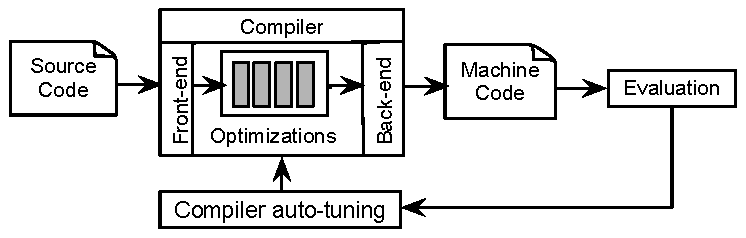
\includegraphics[width=0.9\linewidth]{chapitre3/fig/autotuning.pdf}
	\caption{Process of compiler optimization exploration}
	
\end{figure}

\subsection{Example: GCC Compiler}
\begin{table}
	\label{table:options}
	\centering
	\caption{Compiler optimization options enabled by GCC standard levels}
	\scalebox{0.88}{
		\begin{tabular}[c]{|c|p{7cm}||c|p{7cm}|}
			\cline{1-4}
			\textbf{Level} & \textbf{Optimization option} & \textbf{Level} & \textbf{Optimization option}  \\
			\hline
			O1 & 
			-fauto-inc-dec \newline
			-fcompare-elim \newline
			-fcprop-registers \newline
			-fdce \newline
			-fdefer-pop \newline
			-fdelayed-branch \newline
			-fdse \newline
			-fguess-branch-probability \newline
			-fif-conversion2 \newline
			-fif-conversion \newline
			-fipa-pure-const \newline
			-fipa-profile \newline
			-fipa-reference\newline 
			-fmerge-constants\newline 
			-fsplit-wide-types \newline
			-ftree-bit-ccp \newline
			-ftree-builtin-call-dce \newline
			-ftree-ccp \newline
			-ftree-ch \newline
			-ftree-copyrename \newline
			-ftree-dce \newline
			-ftree-dominator-opts \newline
			-ftree-dse \newline
			-ftree-forwprop \newline
			-ftree-fre \newline
			-ftree-phiprop \newline
			-ftree-slsr \newline
			-ftree-sra \newline
			-ftree-pta \newline
			-ftree-ter \newline
			-funit-at-a-time
			
			&
			\multirow{2}{*}{O2} & \multirow{2}{6cm} {
				-fthread-jumps\newline 
				-falign-functions\newline  
				-falign-jumps \newline
				-falign-loops  \newline
				-falign-labels \newline
				-fcaller-saves \newline
				-fcrossjumping \newline
				-fcse-follow-jumps  \newline
				-fcse-skip-blocks \newline
				-fdelete-null-pointer-checks \newline
				-fdevirtualize \newline
				-fexpensive-optimizations \newline
				-fgcse  \newline
				-fgcse-lm  \newline
				-fhoist-adjacent-loads \newline
				-finline-small-functions \newline
				-findirect-inlining \newline
				-fipa-sra \newline
				-foptimize-sibling-calls \newline
				-fpartial-inlining \newline
				-fpeephole2 \newline
				-fregmove \newline
				-freorder-blocks  \newline
				-freorder-functions \newline
				-frerun-cse-after-loop \newline 
				-fsched-interblock \newline 
				-fsched-spec \newline
				-fschedule-insns  \newline
				-fschedule-insns2 \newline
				-fstrict-aliasing \newline
				-fstrict-overflow \newline
				-ftree-switch-conversion\newline -ftree-tail-merge \newline
				-ftree-pre \newline
				-ftree-vrp
			} \\
			\cline{1-2}
			O3 & 
			-finline-functions \newline
			-funswitch-loops\newline
			-fpredictive-commoning \newline
			-fgcse-after-reload \newline
			-ftree-vectorize \newline
			-fvect-cost-model \newline
			-ftree-partial-pre \newline 
			-fipa-cp-clone  & &  \\
			\cline{1-2}
			Ofast & -ffast-math &   &  \\
			\hline
			
		\end{tabular}
	}
\end{table}

The GNU Compiler Collection, GCC, is a very popular collection of programming compilers, available for different platforms.
GCC exposes its various optimizations via a number of flags that can be turned on or off through command-line compiler switches. 

For instance, version 4.8.4 provides a wide range of command-line options that can be enabled or disabled, including more than 150 options for optimization. The diversity of available optimization options makes the design space for optimization level very huge, increasing the need for heuristics to explore the search space of feasible optimization sequences.

As it is shown in Table 4.1, we count 76 optimization flags that are enabled by the four default optimization levels (O1, O2, O3, Ofast). 

Each standard level is composed by a number of optimizations. These levels are defined by compiler designers based on their experiences and preliminary experiments. The goal of defining these standard levels is to build general and program independent sequences that represent trade-offs among several non-functional properties.

For instance, O1 enables the optimization flags that reduce the code size and execution time without performing any optimization that reduces the compilation time. It turns on 32 flags. 
O2 increases the compilation time and reduces the execution time of generated code. It turns on all optimization flags specified by O1 plus 35 other options. 
O3 is more aggressive level which enables all O2 options plus 8 more optimizations. 
Finally, Ofast is the most aggressive level which enables optimizations that are not valid for all standard-compliant programs. It turns on all O3 optimizations plus one more aggressive optimization. 
This results in a huge space with $2^{76}$ possible optimization combinations.
The full list of optimizations is available here~\cite{mboussaa}.
%In our approach, we did not consider some optimization options that are enabled by default, since they do not affect the performance of generated binaries.

Optimization flags in GCC can be turned off by using \textit{"-fno-"}+flag instead of \textit{"-f"}+flag in the beginning of each optimization. 
We use this technique to play with compiler switches.



\section{Evolutionary Exploration of Compiler Optimizations }
Many techniques (meta-heuristics, random search, etc.) can be used to explore the large set of optimization combinations of modern compilers. 
In our approach, we particularly study the use of the Novelty Search technique to identify the set of compiler optimization options that optimize the non-functional properties of code.

\subsection{Novelty Search Adaptation}

In this work, we aim at providing a new alternative for choosing effective compiler optimization options compared to the state of the art approaches. 
In fact, since the search space of possible combinations is too large, we aim at using a new search-based technique called Novelty Search~\cite{lehman2008exploiting} to tackle this issue. 
The idea of this technique is to explore the search space of possible compiler flag options by considering sequence diversity as a single objective. 
Instead of having a fitness-based selection that maximizes one of the non-functional objectives, we select optimization sequences based on a novelty score showing how different they are compared to all other combinations evaluated so far. 

NS is a divergent evolutionary algorithm which rewards optimization sequences that diverge from previously discovered ones. Thus, evolution can be viewed as a divergent process compared to the traditional convergent approaches that exert the selection pressure based on fitness values.

Moreover, we claim that the search towards effective optimization sequences is not straightforward since the interactions between optimizations is too complex and difficult to define. 

For instance, in a previous work~\cite{chen2012deconstructing}, Chen et al. showed that handful optimizations may lead to higher performance than other techniques of iterative optimization. 
In fact, the fitness-based search may be trapped into some local optima that cannot escape\cite{bodin1998iterative}. 
This phenomenon is known as \textit{"diversity loss"}. For example, if the most effective optimization sequence that induces less execution time lies far from the search space defined by the gradient of the fitness function, then some promising search areas may not be reached. 
The issue of premature convergence to local optima has been a common problem in evolutionary algorithms. 
Many methods are proposed to overcome this problem~\cite{banzhaf1996effect}. 
However, all these efforts use a fitness-based selection to guide the search. Considering diversity as the unique objective function to be optimized may be a key solution to this problem.

Therefore, during the evolutionary process, we select optimization sequences that remain in sparse regions of the search space in order to guide the search towards novelty. 
In the meantime, we choose to gather the non-functional metrics relative to the resource consumption (memory and CPU usage) of optimized code. 
We describe in more details the way we are collecting these non-functional metrics in section 4.4.

\begin{algorithm}
	\algsetup{linenosize=\tiny}
	\footnotesize
	%footnotesize
	\caption{Novelty search algorithm for compiler optimization exploration}
	\label{algo:search}
	\begin{algorithmic}[1]
		
		\REQUIRE Optimization options $\mathcal{O}$
		\REQUIRE Program $\mathcal{C}$
		\REQUIRE Novelty threshold $\mathcal{T}$
		\REQUIRE Limit $\mathcal{L}$
		\REQUIRE Nearest neighbors $\mathcal{K}$
		\REQUIRE Number of evaluations $\mathcal{N}$
		\ENSURE Best optimization sequence $best\_sequence$
		\STATE $initialize\_parameters(\mathcal{L},\mathcal{T},\mathcal{N},\mathcal{K})$
		\STATE $create\_archive(\mathcal{L})$
		\STATE 	$generated\_code \gets compile(\textit{"-O0"},\mathcal{C})$
		\STATE 	$minimum\_usage \gets execute(generated\_code)$
		\STATE $population \gets random\_sequences(\mathcal{O})$
		\REPEAT
		\FOR{$sequence \in population$}   
		\STATE 	$generated\_code \gets compile(sequence,\mathcal{C})$
		\STATE 	$memory\_usage \gets execute(generated\_code)$
		\STATE	$novelty\_metric(sequence) \gets distFromKnearest(archive,population,\mathcal{K})$
		\IF{$novelty\_metric > \mathcal{T}$}
		\STATE	$archive \gets archive \cup sequence$
		\ENDIF
		
		\IF{$memory\_usage < minimum\_usage$}
		\STATE	$best\_sequence \gets sequence$
		\STATE	$minimum\_usage \gets memory\_usage$
		\ENDIF
		
		\ENDFOR
		\STATE		$new\_population \gets generate\_new\_population(population)$
		\STATE		$generation \gets generation + 1$
		\UNTIL{$generation = \mathcal{N}$}
		\RETURN $best\_sequence$
	\end{algorithmic}
\end{algorithm}

Generally, NS acts like GAs (Example of GA use in  \cite{cooper2002adaptive}). However, NS needs extra changes. First, a new novelty metric is required to replace the fitness function. Then, an archive must be added to the algorithm, which is a kind of a database that remembers individuals that were highly novel when they were discovered in past generations. 
Algorithm~\ref{algo:search} describes the overall idea of our NS adaptation. The algorithm takes as input a source code program and a list of optimizations. 

We initialize first the novelty parameters and create a new archive with limit size L (lines 1 \& 2). In this example, we gather information about memory consumption. In lines 3 \& 4, we compile and execute the input program without any optimization (O0). Then, we measure the resulting memory consumption. By doing so, we will be able to compare it to the memory consumption of new generated solutions. The best solution is the one that yields to the lowest memory consumption compared to O0 usage.

Before starting the evolutionary process, we generate an initial population with random sequences. Line 6-21 encode the main NS loop, which searches for the best sequence in terms of memory consumption. For each sequence in the population, we compile the input program, execute it and evaluate the solution by calculating the average distance from its k-nearest neighbors. Sequences that get a novelty metric higher than the novelty threshold T are added to the archive. T defines the threshold for how novel a sequence has to be before it is added to the archive. In the meantime, we check if the optimization sequence yields to the lowest memory consumption so that, we can consider it as the best solution. 

Finally, genetic operators (mutation and crossover) are applied afterwards to fulfill the next population. This process is iterated until reaching the maximum number of evaluations.


\subsubsection{Optimization Sequence Representation}
For our case study, a candidate solution represents all compiler switches that are used in the four standard optimization levels (O1, O2, O3 and Ofast). Thereby, we represent this solution as a vector where each dimension is a compiler flag. 
The variables that represent compiler options are represented as genes in a chromosome. 
Thus, a solution represents the CFLAGS value used by GCC to compile programs.
A solution has always the same size, which corresponds to the total number of involved flags. 
However, during the evolutionary process, these flags are turned on or off depending on the mutation and crossover operators (see example in Figure 4.2). As well, we keep the same order of invoking compiler flags since that does not affect the optimization process and it is handled internally by GCC.

\begin{figure}[h]
	\centering
	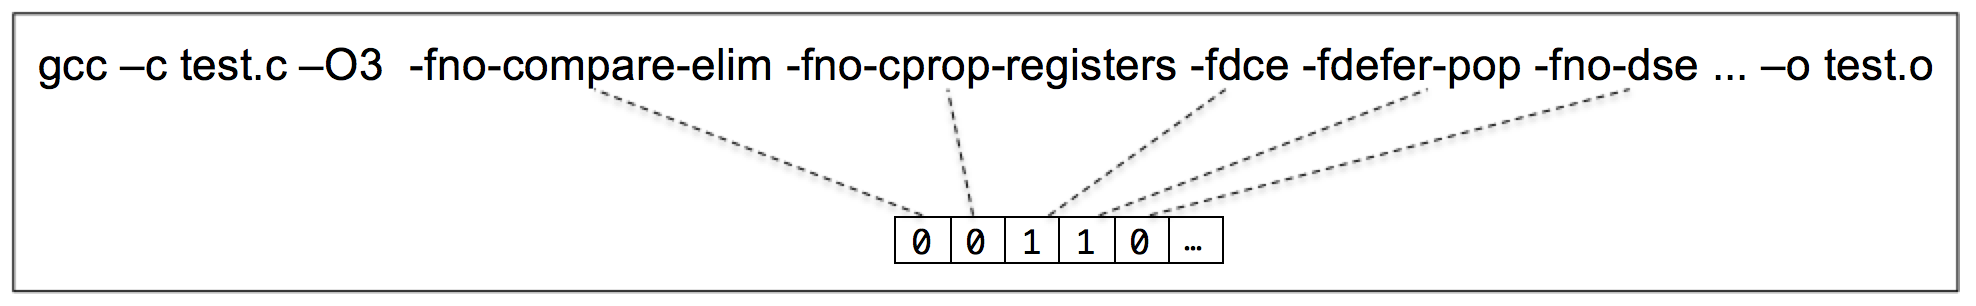
\includegraphics[width=1\hsize]{chapitre3/fig/individual.png}
	\caption{Solution representation}	
\end{figure}

\subsubsection{Novelty Metric}
The Novelty metric expresses the sparseness of an input optimization sequence. It measures its distance to all other sequences in the current population and to all sequences that were discovered in the past (\ie, sequences in the archive). 
We can quantify the sparseness of a solution as the average distance to the k-nearest neighbors. 

If the average distance to a given point's nearest neighbors is large then it belongs to a sparse area and will get a high novelty score. 
Otherwise, if the average distance is small so it belongs certainly to a dense region then it will get a low novelty score. 
The distance between two sequences is computed as the total number of symmetric differences among optimization sequences. Formally, we define this distance as follows :

\begin{equation}
distance(S1,S2)=\left | S1 \bigtriangleup S2 \right |
\end{equation}

where $S1$ and $S2$ are two selected optimization sequences (solutions). The distance value is equal to 0 if the two optimization sequences are similar and higher than 0 if there is at least one optimization difference. The maximum distance value is equal to the total number of input flags.

To measure the sparseness of a solution, we use the previously defined distance to compute the average distance of a sequence to its k-nearest neighbors. In this context, we define the novelty metric of a particular solution as follows:

\begin{equation}
NM(S) = \frac{1}{k} \sum_{i=1}^{k} distance(S,\mu _{i})
\end{equation}

where $\mu _{i}$ is the $i^{th}$ nearest neighbor of the solution S within the population and the archive of novel individuals. 

\subsection{Novelty Search For Multi-objective Optimization}
A multi-objective approach provides a trade-off between two objectives where the developers can select their desired solution from the Pareto-optimal front. The idea of this approach is to use multi-objective algorithms to find trade-offs between non-functional properties of generated code such as \textit{$<$ExecutionTime--MemoryUsage$>$}. The correlations we are trying to investigate are more related to the trade-offs between resource consumption and execution time.

For instance, NS can be easily adapted to multi-objective problems. In this adaptation, the SBSE formulation remains the same as described in Algorithm 1. However, in order to evaluate the new discovered solutions, we have to consider two main objectives and add the non-dominated solutions to the Pareto non-dominated set. We apply the Pareto dominance relation to find solutions that are not Pareto dominated by any other solution discovered so far, like in NSGA-II~\cite{lokuciejewski2010multi, deb2002fast}. Then, this Pareto non-dominated set is returned as a result.
There is typically more than one optimal solution at the end of NS. The maximum size of the final Pareto set cannot exceed the size of the initial population.


\section{Evaluation}
So far, we have presented a sound procedure for auto-tuning compilers through the use of NS. In this section, we evaluate the implementation of our approach by explaining the design of our empirical study; the research questions we set out to answer and different methods we used to answer these questions. The experimental material is available for replication purposes\footnote{https://noticegcc.wordpress.com/}.

\subsection{Research Questions}
Our experiments aim at answering the following research questions:

\textbf{RQ1: Mono-objective SBSE Validation.} 
\textit{How does the proposed diversity-based exploration of optimization sequences perform compared to other mono-objective algorithms in terms of memory and CPU consumption, execution time, etc.?} 


\textbf{RQ2: Sensitivity.} 
\textit{How sensitive are input programs to compiler optimization options?}


\textbf{RQ3: Impact of optimizations on resource consumption.} 
\textit{How compiler optimizations impact on the non-functional properties of generated programs?}


\textbf{RQ4: Trade-offs between non-functional properties.} 
\textit{How can multi-objective approaches be useful to find trade-offs between non-functional properties?}

To answer these questions, we conduct several experiments using NOTICE to validate our global approach for non-functional testing of compilers using system containers.


\subsection{Experimental Setup}
\subsubsection{Programs Used in the Empirical Study}
To explore the impact of compiler optimizations a set of input programs are needed. 
To this end, we use a random C program generator called Csmith~\cite{yang2011finding}.
Csmith is a tool that can generate random C programs that statically and dynamically conform to the C99 standard. It has been widely used to perform functional testing of compilers~\cite{chen2016empirical,le2014compiler,nagai2013scaling} but not the case for checking non-functional requirements. Csmith can generate C programs that use a much wider range of C features including complex control flow and data structures such as pointers, arrays, and structs. 

Csmith programs come with their test suites that explore the structure of generated programs (i.e., high quality code coverage).
Yang et al.~\cite{yang2011finding} argue that Csmith is an effective bug-finding tool because it generates tests that explore atypical combinations of C language features. They also argue that larger programs are more effective for functional testing. 

Thus, we run Csmith for 24 hours and gathered the largest generated programs. We depicted 111 C programs with an average number of source lines of 12K. 10 programs are used as training set for RQ1, 100 other programs to answer RQ2 and one last program to run RQ4 experiment.

The selected Csmith programs are described in more details at~\cite{mboussaa}.

%Moreover, we run experiments on commonly used benchmarks in iterative compilation named Collective Benchmark (Cbench)~\cite{fursin2009collective}. It is a collection of open-source sequential programs in C, targeting specific areas of the embedded market. It comes with multiple datasets assembled by the community to enable realistic benchmarking and research on program and architecture optimization. Cbench contains more than 20 C programs. 


Moreover, we run experiments on commonly used benchmarks named Collective Benchmark (cBench)~\cite{fursin2009collective}. It is a collection of open-source sequential programs in C targeting specific areas of the embedded market. It comes with multiple datasets assembled by the community to enable realistic benchmarking and research on program and architecture optimization. cBench contains more than 20 C programs. The following table describes programs that we have selected from this benchmark to evaluate our approach.

These real world benchmark programs are used to study the influence of compiler optimizations on the resource usage in RQ3 experiments.
 
\begin{table}[h]
	\begin{center}
		\begin{tabular}{|c|c|p{5cm}|}
			\hline
			\textbf{Program} & \textbf{Source lines} & \textbf{Description}\\
			\hline
			automative\_susan\_s & 1376 & Image recognition package\\
			\hline
			bzip2e & 5125 & Compress any file
			source code \\
			\hline
			bzip2d & 5125 & Decompress zipped files \\
			\hline
			office\_rsynth & 4111 & Text to speech program produced by integrating various pieces of code\\
			\hline
			consumer\_tiffmedian& 15870 & Apply the median cut algorithm to data in a TIFF file
			\\
			
			\hline
			consumer\_tiffdither& 15399 & Convert a greyscale image to bilevel using dithering
			\\
			\hline
			
		\end{tabular}
		
	\end{center}
	\caption {Description of selected benchmark programs}
\end{table}


\subsubsection{Parameters Tuning}
An important aspect for meta-heuristic search algorithms lies in the parameters tuning and selection, which are necessary to ensure not only fair comparison, but also for potential replication.
NOTICE implements three mono-objective search algorithms (Random Search (RS), NS, and GA~\cite{cooper2002adaptive}) and two multi-objective optimizations (NS and NSGA-II~\cite{deb2002fast}). Each initial population/solution of different algorithms is completely random. The stopping criterion is when the maximum number of fitness evaluations is reached.
The resulting parameter values are listed in Table 4.3. The same parameter settings are applied to all algorithms under comparison.

NS, which is our main concern in this work, is implemented as described in Section 3. During the evolutionary process, each solution is evaluated using the novelty metric. Novelty is calculated for each solution by taking the mean of its 15 nearest optimization sequences in terms of similarity (considering all sequences in the current population and in the archive). Initially, the archive is empty. Novelty distance is normalized in the range [0-100].
Then, to create next populations, an elite of the 10 most novel organisms is copied unchanged, after which the rest of the new population is created by tournament selection according to novelty (tournament size = 2). Standard genetic programming crossover and mutation operators are applied to these novel sequences in order to produce offspring individuals and fulfill the next population (crossover = 0.5, mutation = 0.1).
In the meantime, individuals that get a score higher than 30 (threshold T), they are automatically added to the archive as well. 
In fact, this threshold is dynamic. Every 200 evaluations, we check how many individuals have been copied into the archive. If this number is below 3, the threshold is increased by multiplying it by 0.95, whereas if solutions added to archive are above 3, the threshold is decreased by multiplying it by 1.05. 
Moreover, as the size of the archive grows, the nearest-neighbor calculation that determines the novelty scores for individuals becomes more computationally demanding. So, to avoid having low accuracy of novelty, we choose to limit the size of the archive (archive size = 500). Hence, it follows a first-in first-out data structure which means that when a new solution gets added, the oldest solution in the novelty archive will be discarded. Thus, we ensure individual diversity by removing old sequences that may no longer be reachable from the current population.

Algorithm parameters were tuned individually in preliminary experiments. For each parameter, a set of values was tested. The parameter values chosen are the mostly used in the literature~\cite{inden2013examination}. The value that yielded the highest performance score was chosen.  

\begin{table}
	\centering
	\caption{Algorithm parameters}
	\begin{tabular}{| l |l| l |l| }\hline
		\textbf{Parameter} & \textbf{Value} & \textbf{Parameter} & \textbf{Value} \\	\hhline{|=|=|=|=|}	
		Novelty nearest-k  & 15 &  Tournament size & 2\\ 
		Novelty threshold & 30 &  Mutation prob. & 0.1\\  
		Max archive size & 500 &  Crossover & 0.5  \\  
		Population size & 50 &  Nb generations &  100 \\  
		Individual length & 76 & Elitism & 10  \\ 
		Scaling archive prob. & 0.05 & Solutions added to archive & 3  \\ 	\hline
	\end{tabular}
\end{table}

\subsubsection{Evaluation Metrics Used}

For mono-objective algorithms, we use to evaluate solutions using the following metrics:

-\textit{Memory Consumption Reduction (MR)}: corresponds to the percentage ratio of memory usage reduction of running container over the baseline. The baseline in our experiments is O0 level, which means a non-optimized code. Larger values for this metric mean better performance. Memory usage is measured in bytes.

-\textit{CPU Consumption Reduction (CR)}: corresponds to the percentage ratio of CPU usage reduction over the baseline. Larger values for this metric mean better performance. The CPU consumption is measured in seconds, as the CPU time.

-\textit{Speedup (S)}: corresponds to the percentage improvement in execution speed of an optimized code compared to the execution time of the baseline version. Program execution time is measured in seconds.


%When comparing two mono-objective algorithms, it is usual to compare their best solutions found so far during the optimization process. However, this is not applicable when comparing two multi-objective evolutionary algorithms since each of them gives as output a set of non-dominated (Pareto equivalent) solutions. For this reason, we use performance indicator to compare multi-objective algorithms.
%Thus, for multi-objective algorithms we use to evaluate solutions using the following metric:

%-\textit{Hypervolume (HV)}: corresponds to the proportion of objective space that is dominated by the Pareto front approximation returned by the algorithm and delimited by a reference point. The HV reference point is the point obtained by taking the maximum value observed. Thus, the HV metric can be computed as the area between the Pareto frontier and the HV reference point. Larger values for this metric mean better performance. The most interesting features of this indicator are its Pareto dominance compliance and its ability to capture both convergence and diversity~\cite{deb2001multi}. 

\subsubsection{Setting up Infrastructure}
To answer the previous research questions, we configure NOTICE to run different experiments. Figure 4.3 shows a big picture of the testing and monitoring infrastructure considered in these experiments. 

First, a meta-heuristic (mono or multi-objective) is applied to generate specific optimization sequences for the GCC compiler (step 1).

During all experiments, we use GCC 4.8.4, as it is introduced in the motivation section, although it is possible to choose another compiler version using NOTICE since the process of optimizations extraction is done automatically. 

Then, we generate a new optimized code and deploy the output binary within a new instance of our preconfigured Docker image (step 2). While executing the optimized code inside the container, we collect runtime performance data (step 4) and record it in a new time-series database using our InfluxDB back-end container (step 5). 

Next, NOTICE accesses remotely to stored data in InfluxDB using HTTP request calls and assigns new performance values to the current solution (step 6). 

The choice of performance metrics depends on experiment objectives (Memory improvement, speedup, etc.).

More details about the container-based infrastructure and the technical choices are provided in chapter 5.

\begin{figure}[h]
	\centering
	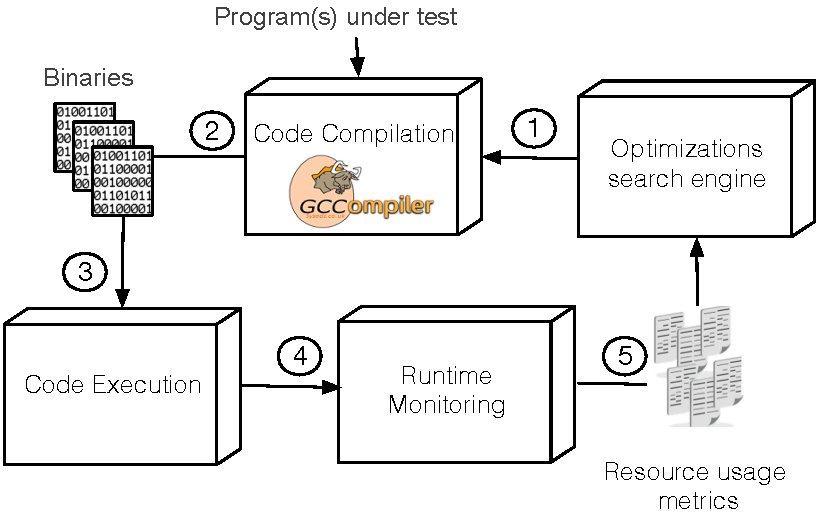
\includegraphics[width=0.8\linewidth]{chapitre3/fig/infraup.pdf}
	\caption{NOTICE experimental infrastructure}
\end{figure}

To obtain comparable and reproducible results, we use the same hardware across all experiments: an AMD A10-7700K APU Radeon(TM) R7 Graphics processor with 4 CPU cores (2.0 GHz), running Linux with a 64 bit kernel and 16 GB of system memory.


\subsection{Experimental Methodology and Results}
In the following paragraphs, we report the methodology and results of our experiments.

\subsubsection{RQ1. Mono-objective SBSE Validation}
\paragraph{Method}

To answer the first research question RQ1, we conduct a mono-objective search for compiler optimization exploration in order to evaluate the non-functional properties of optimized code. Thus, we generate optimization sequences using three search-based techniques (RS, GA, and NS) and compare their performance results to standard GCC optimization levels (O1, O2, O3, and Ofast). 

In this experiment, we choose to optimize for execution time (S), memory usage (MR), and CPU consumption (CR). Each non-functional property is improved separately and independently of other metrics. We recall that other properties can be also optimized using NOTICE (e.g., code size, compilation time, etc.), but in this experiment, we focus only on three properties.


\begin{figure}[h]
	\centering
	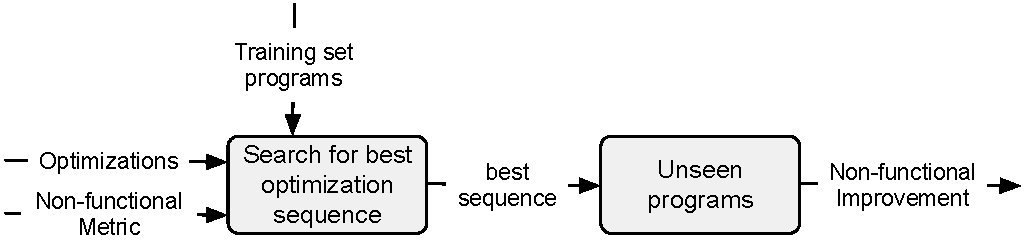
\includegraphics[width=1.\linewidth]{chapitre3/fig/sensitivity.pdf}
	\caption{Evaluation strategy to answer RQ1 and RQ2}
	
\end{figure}


As it is shown on the left side of Figure 4.4, given a list of optimizations and a non-functional objective, we use NOTICE to search for the best optimization sequence across a set of input programs that we call \textit{"the training set"}. This \textit{"training set"} is composed of random Csmith programs (10 programs). We apply then generated sequences to these programs. Therefore, the code quality metric, in this setting, is equal to the average performance improvement (S, MR, or CR) and that, for all programs under test. 


To summarize, in this experiment we aim to: (1) compare the performance of our proposed diversity-based exploration of optimization sequences (NS) to GA and RS; and (2) demonstrate that NOTICE is able to find the optimal solution relative to the input training set.

\paragraph{Results}

\begin{table}[h]
	\centering
	\caption{Results of mono-objective optimizations}
	\label{my-label}
	\begin{tabular}{|l|l|l|l|l|l|l|c|}
		\hline
		& \textbf{O1}                    & \textbf{O2}                    & \textbf{O3}                    & \textbf{Ofast}                 & \textbf{RS}                    & \textbf{GA}                    & 
		\textbf{NS} \\
		\hhline{|=|=|=|=|=|=|=|=|}
		S  &  1.051 & 1.107  & 1.107  & 1.103  & 1.121  &  1.143 &  1.365  \\ \hline
		MR(\%) & 4.8  & -8.4  &  4.2 & 6.1  &  10.70 & 15.2  &  15.6  \\ \hline
		CR(\%) & -1.3  & -5  & 3.4  & -5  &  18.2 & 22.2  &  23.5  \\ \hline
	\end{tabular}
\end{table}

Table 4.4 reports the comparison results of three non-functional properties CR, MR, and S. At the first glance, we can clearly see that all search-based algorithms outperform standard GCC levels with minimum improvement of 10\% for memory usage and 18\% for CPU time (when applying RS).
 
Our proposed NS approach has the best improvement results for three metrics with 1.365 of speedup, 15.6\% of memory reduction and 23.5\% of CPU time reduction across all programs under test. NS is clearly better than GA in terms of speedup. However, for MR and CR, NS is slightly better than GA with 0.4\% improvement for MR and 1.3\% for CR. RS has almost the lowest optimization performance but is still better than standard GCC levels.

We remark as well that applying standard optimizations has an impact on the execution time with a speedup of 1.107 for O2 and O3. Ofast has the same impact as O2 and O3 for the execution speed. However, the impact of GCC levels on resource consumption is not always efficient. O2, for example, increases resource consumption compared to O0 (-8.4\% for MR and -5\% for CR). 

This can be explained by the fact that standard GCC levels apply some aggressive optimizations that increase the performance of generated code and deteriorate system resources.  

\noindent\fbox{\parbox{\linewidth-2\fboxrule-2\fboxsep}{
		\textbf{Key findings for RQ1.} \\
		-- Best discovered optimization sequences using mono-objective search techniques always provide better results than standard GCC optimization levels.\\
		-- Novelty Search is a good candidate to improve code in terms of non-functional properties since it is able to discover optimization combinations that outperform RS and GA.  }}


\subsubsection{RQ2. Sensitivity}
\paragraph{Method}
Another interesting experiment is to test the sensitivity of input programs to compiler optimizations and evaluate the general applicability of best optimal optimization sets, previously discovered in RQ1. These sequences correspond to the best generated sequences using NS for the three non-functional properties S, MR and CR (i.e., sequences obtained in column 8 of Table 4.4). 

Thus, we apply best discovered optimizations in RQ1 to new unseen Csmith (100 new random programs) and we compare then, the performance improvement across these programs (see right side of Figure 4.4). We also apply standard optimizations, O2 and O3, to new Csmith programs in order to compare the performance results.
The idea of this experiment is to test whether new generated Csmith programs are sensitive to previously discovered optimizations or not. 

If so, this will be useful for compiler users and researchers to use NOTICE in order to build general optimization sequences from their representative \textit{training set} programs.

\begin{figure}[h]
	\centering
	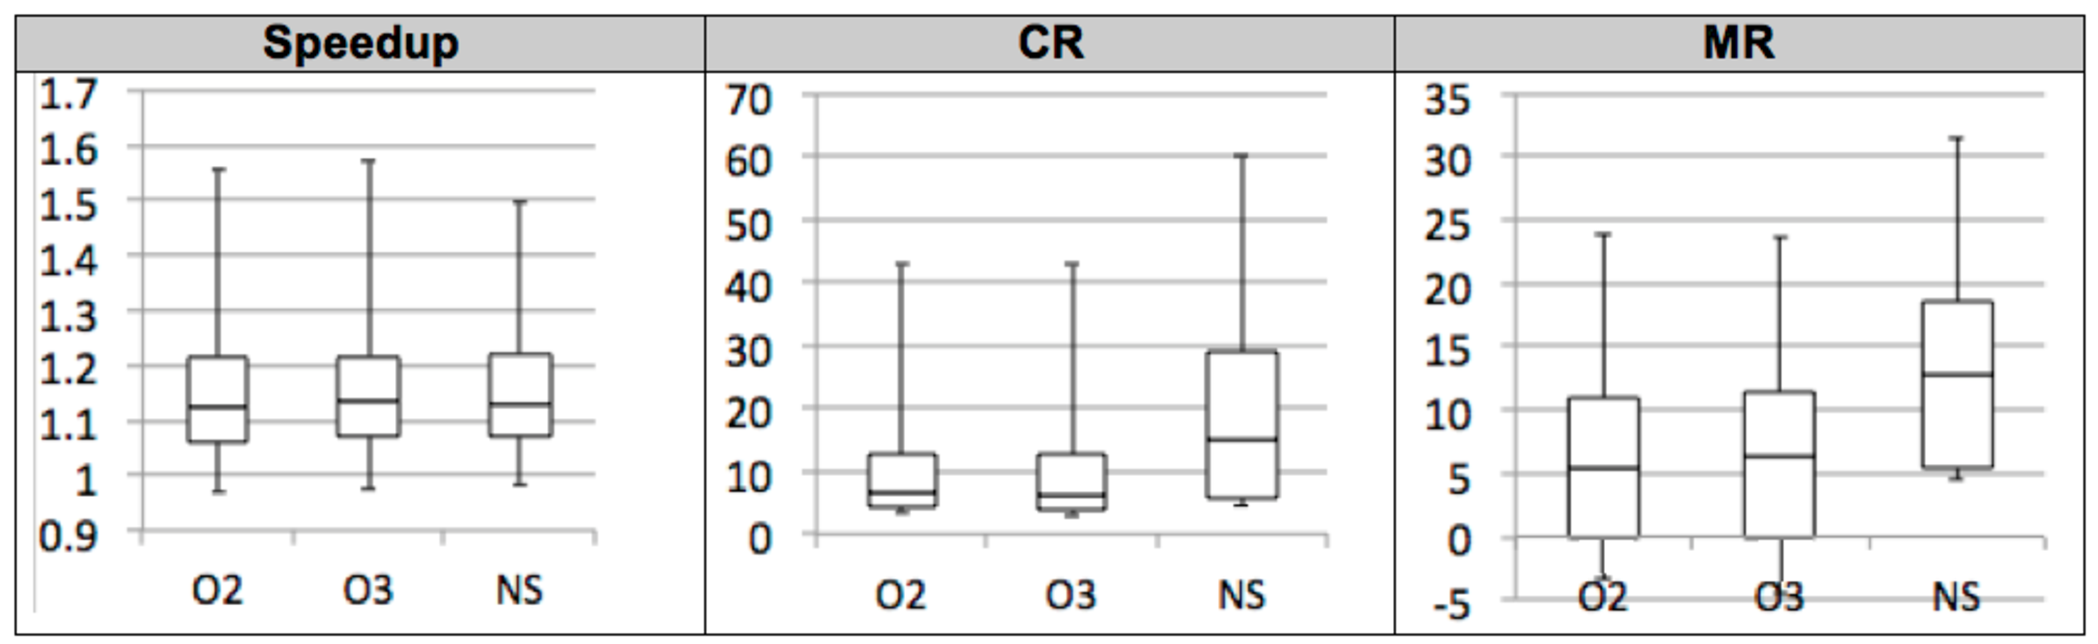
\includegraphics[width=1.\linewidth]{chapitre3/fig/box.pdf}
	\caption{Boxplots of the obtained performance results across 100 unseen Csmith programs, for each non-functional property: Speedup (S), memory (MR) and CPU (CR) and for each optimization strategy: O2, O3 and NS}
\end{figure}

\paragraph{Results}
Figure 4.5 shows the distribution of memory, CPU and speedup improvement across 100 new Csmith programs. For each non-functional property, we apply O2, O3 and best NS sequences. Speedup results show that the three optimization strategies lead to almost the same distribution with a median value of 1.12 for speedup. 

This can be explained by the fact that NS might need more time to find the sequence that best optimizes the execution speed. Meanwhile, O2 and O3 have also the same impact on CR and MR which is almost the same for both levels (CR median value is 8\% and around 5\% for MR).

However, the impact of applying best generated sequences using NS clearly outperforms O2 and O3 with almost 10\% of CPU improvement and 7\% of memory improvement. 

This proves that NS sequences are efficient and can be used to optimize resource consumption of new Csmith programs. This result also proves that Csmith code generator applies the same rules and structures to generate C code. For this reason, applied optimization sequences always have a positive impact on the non-functional properties.

\noindent\fbox{\parbox{\linewidth-2\fboxrule-2\fboxsep}{
		\textbf{Key findings for RQ2.}\\
		-- It is possible to build general optimization sequences that perform better than standard optimization levels \\
		-- Best discovered sequences in RQ1 can be mostly used to improve the memory and CPU consumption of Csmith programs. To answer RQ2, Csmith programs are sensitive to compiler optimizations.}}


\subsubsection{RQ3. Impact of optimizations on resource usage}
In this experiment, we evaluate the impact of applying the standard optimization levels and the new discovered sequences on the resource usage. We also study the correlation between speedup and resource consumption of generated code. 

The idea of this experiment is to: (1) prove, or not, the usefulness of involving resource usage metrics as key objectives for performance improvement; (2) the need, or not, of multi-objective search strategy to handle the different non-functional requirements such as resource usage and performance properties.

In the following, we describe two methods to run experiments. The first is based on Csmith programs and the second is based on Cbench programs.

\paragraph{Method 1}

In this experiment, we use NOTICE to provide an understanding of optimizations impact, in terms of resource consumption, when trying to optimize for execution time. 

Thus, we choose one instance of obtained results in RQ1 related to the best speedup improvement (i.e., results obtained in line 1 of Table 4.4) and we study the impact of speedup improvement on memory and CPU consumption. We also compare the resource usage data to standard GCC levels as they were presented in Table 4.4. Improvements are always calculated over the non-optimized version (O0). The following measurements are based on the training set of 10 Csmith programs.

\paragraph{Results 1}

Figure 4.6 shows the impact of speedup optimization on resource consumption. For instance, O2 and O3 that led to the best speedup improvement among standard optimization levels in RQ1, present opposite impact on resource usage. Applying O2 induces -8.4\% of MR and -5\% of CR. However, applying O3 improves MR and CR respectively by 3.4\% and 4.2\%. Hence, we note that when applying standard levels, there is no clear correlation between speedup and resource usage since compiler optimizations are generally used to optimize the execution speed and never evaluated to reduce system resources.

On the other hand, the outcome of applying different mono-objective algorithms for speedup optimization also proves that resource consumption is always in conflict with execution speed. The highest MR and CR is reached using NS with respectively 1.2\% and 5.4\%. This improvement is considerably low compared to scores reached when we have applied resource usage metrics as key objectives in RQ1 (i.e., 15.6\% for MR and 23.5\% for CR). Furthermore, we note that generated sequences using RS and GA have a high impact on system resources since all resource usage values are worse than the baseline.

These results agree to the idea that compiler optimizations do not put too much emphasis on the trade-off between execution time and resource consumption.


\begin{figure}[h]
		\centering
		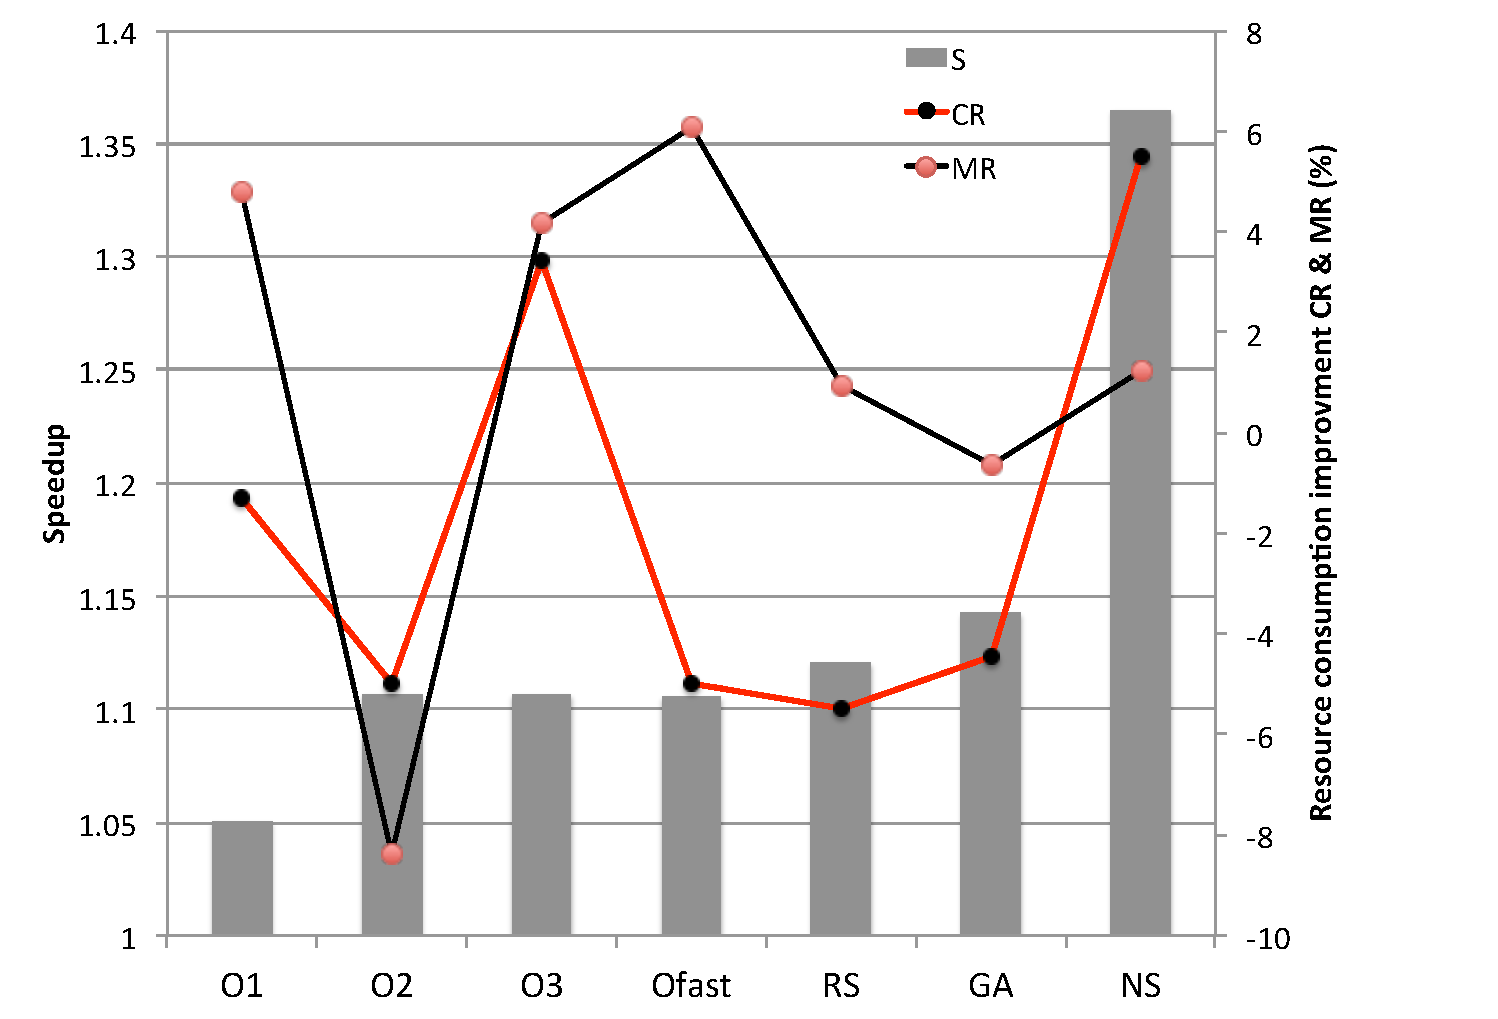
\includegraphics[width=0.9\linewidth]{chapitre3/fig/rq3.pdf}
		\caption{Impact of speedup improvement on memory and CPU consumption for each optimization strategy}
\end{figure}


\paragraph{Method 2}

Now, we study the impact of applying standard levels (01, O2, O3, Ofast) on the memory usage across 5 different Cbench programs. We compare the results with solutions generated using NOTICE which have the best memory consumption reduction (i.e., generated by NS). 

Figure 4.7 shows this comparison across different benchmark programs. It presents the percentage of saved memory of standard and novelty optimizations over O0 level (no optimization applied).

To study the correlation between execution time and memory consumption of running programs, we present in Figure 4.8 an evaluation of the speedup according standard levels. Again, we compare these results to the sequence that had the best memory reduction in Figure 4.7 (i.e., NS solution). 

\paragraph{Results 2}

\begin{figure}[!ht]
	\centering
	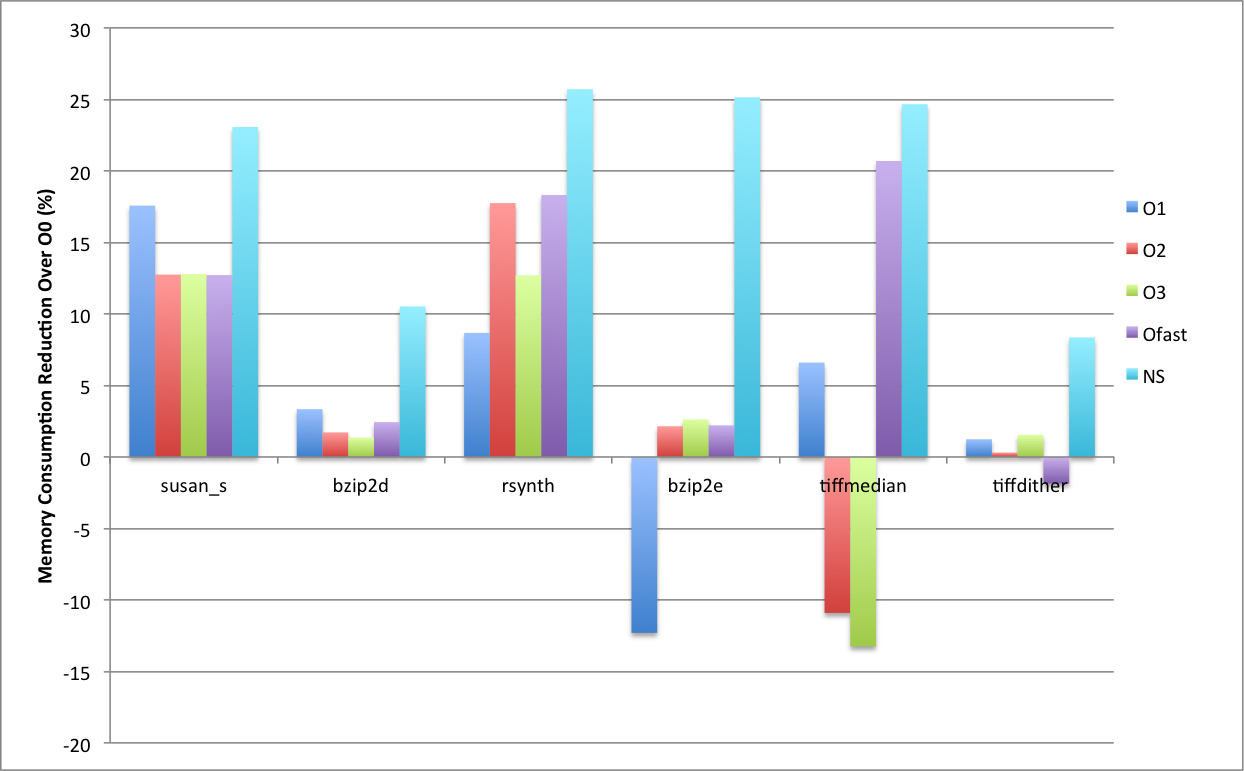
\includegraphics[width=1.\linewidth]{chapitre3/fig/infra_novelty_stat3.png}
	\caption{Evaluating the amount of saved memory after applying standard optimization options compared to best generated optimization using NS}
\end{figure}


As expected, the results show that NS clearly outperforms standard optimizations for all benchmark programs. 

Using NS, we are able to reach a maximum memory consumption reduction of almost 26\% for the case rsynth program against a maximum of 18\% reduction using Ofast option.

We remark as well that the impact of applying standard optimizations on memory consumption for each program differs from one program to another. 

Using O1 for bzip2e and O2, O3 for tiffmedian can even increase the memory consumption by almost 13 \%. 

This agrees to the idea that standard optimizations does not produce always the same impact results on resource consumption and may be highly dependent on the benchmark and the source code they have been tested on. 

\begin{figure}[!ht]
	\centering
	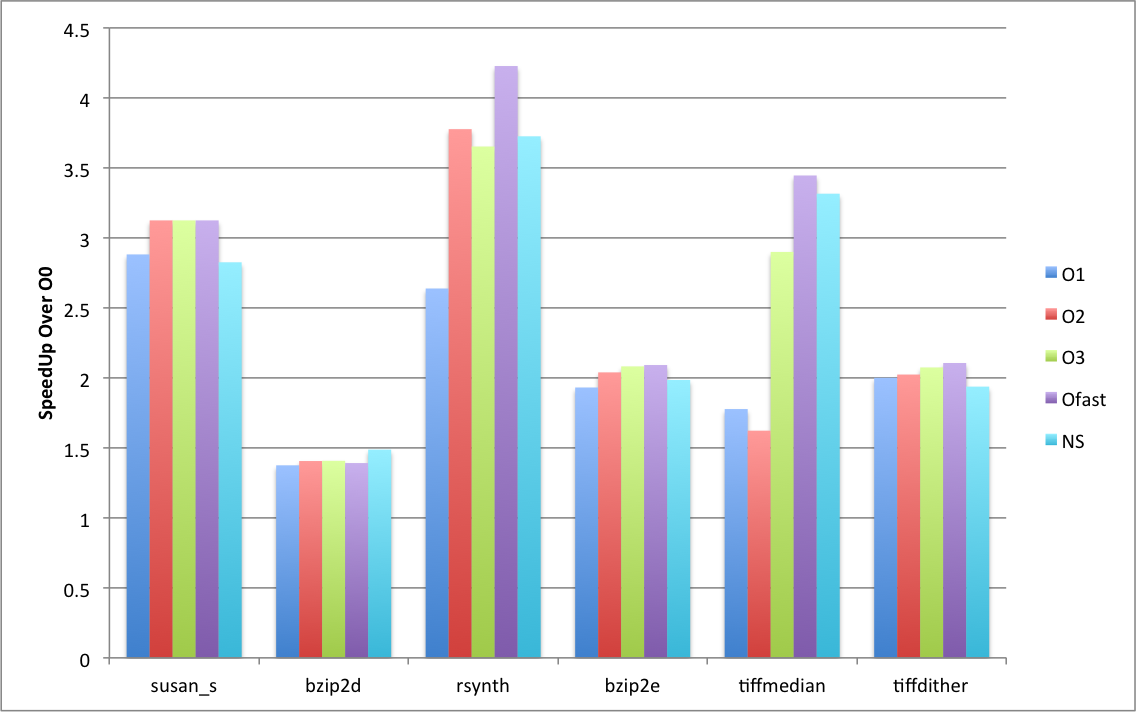
\includegraphics[width=1.\linewidth]{chapitre3/fig/infra_novelty_stat2.png}
	\caption{Evaluating the speedup after applying standard optimization options compared to best generated optimization using NS}
\end{figure}

In Figure 4.8, we can see that optimizations yield to high level of speedup for all benchmark programs (between 1.5 and 4.3).

We can also observe that the different optimization levels do not differ too much in term of execution time. 

We distinguish that Ofast is more efficient for all programs and NS sequence has almost the same speedup as Ofast. 

NS solutions have equal or less performance improvement compared to all standard levels for all benchmarks. 

%The results of this experiments shows that optimizing for memory usage using NS does not affect programs execution time and we demonstrate that we can find optimizations that reduce memory usage while guaranteeing program performance.



\noindent\fbox{\parbox{\linewidth-2\fboxrule-2\fboxsep}{
		\textbf{Key findings for RQ3.} \\
		-- Optimizing software performance can induce undesirable effects on system resources.\\
		-- A trade-off is needed to find a correlation between both, software performance and resource usage.
	}}
	
\subsubsection{RQ4. Trade-offs between non-functional properties}
\paragraph{Method}
Finally, to answer RQ4, we use NOTICE again to find trade-offs between non-functional properties. 

In this experiment, we choose to focus on the trade-off \textit{$<$ExecutionTime--MemoryUsage$>$}. In addition to our NS adaptation for multi-objective optimization, we implement a commonly used multi-objective approach namely NSGA-II~\cite{deb2002fast}. 

We denote our NS adaptation by \textit{NS-II}. We recall that NS-II is not a multi-objective approach as NSGA-II. It uses the same NS algorithm. However, in this experiment, it returns the optimal Pareto front solutions instead of returning one optimal solution relative to one goal. 

Apart from that, we apply different optimization strategies to assess our approach. 	
First, we apply standard GCC levels. Second, we apply best generated sequences relative to memory and speedup optimization (the same sequences that we have used in RQ2). Thus, we denote by \textit{NS-MR} the sequence that yields to the best memory improvement MR and \textit{NS-S} to the sequence that leads to the best speedup. This is useful to compare mono-objective solutions to new generated ones.
	
In this experiment, we assess the efficiency of generated sequences using only one Csmith program.

We evaluate the quality of the obtained Pareto optimal optimization based on raw data values of memory and execution time. Then, we compare qualitatively the results by visual inspection of the Pareto frontiers.

The goal of this experiment is to check whether it exists, or not, a sequence that can reduce both execution time and memory usage.

We report the comparison results of our NS adaptation for optimizations generation to the current state-of-the-art multi-objective approaches namely NSGA-II. 

\paragraph{Results}

Figure 4.9 shows the Pareto optimal solutions that achieved the best performance assessment for the trade-off \textit{$<$ExecutionTime--MemoryUsage$>$}. 
The horizontal axis indicates the memory usage in raw data (in Bytes) as it is collected using NOTICE. In similar fashion, the vertical axis shows the execution time in seconds. Furthermore, the figure shows the impact of applying standard GCC options and best NS sequences on memory and execution time. 

Based on these results, we can see that NSGA-II performs better than NS-II. In fact, NSGA-II yields to the best set of solutions that presents the optimal trade-off between the two objectives. Then, it is up to the compiler user to use one solution from this Pareto front that satisfies his non-functional requirements (six solutions for NSGA-II and five for NS-II). 

For example, he could choose one solution that maximizes the execution speed in favor of memory reduction. 

On the other side, NS-II is capable to generate only one non-dominated solution. For NS-MR, it reduces as expected the memory consumption compared to other optimization levels. The same effect is observed on the execution time when applying the best speedup sequence NS-S. We also note that all standard GCC levels are dominated by our different heuristics NS-II, NSGA-II, NS-S and NS-MR.

This agrees to the claim that standard compiler levels do not present a suitable trade-off between execution time and memory usage.
	
\begin{figure}[h]
		\centering
		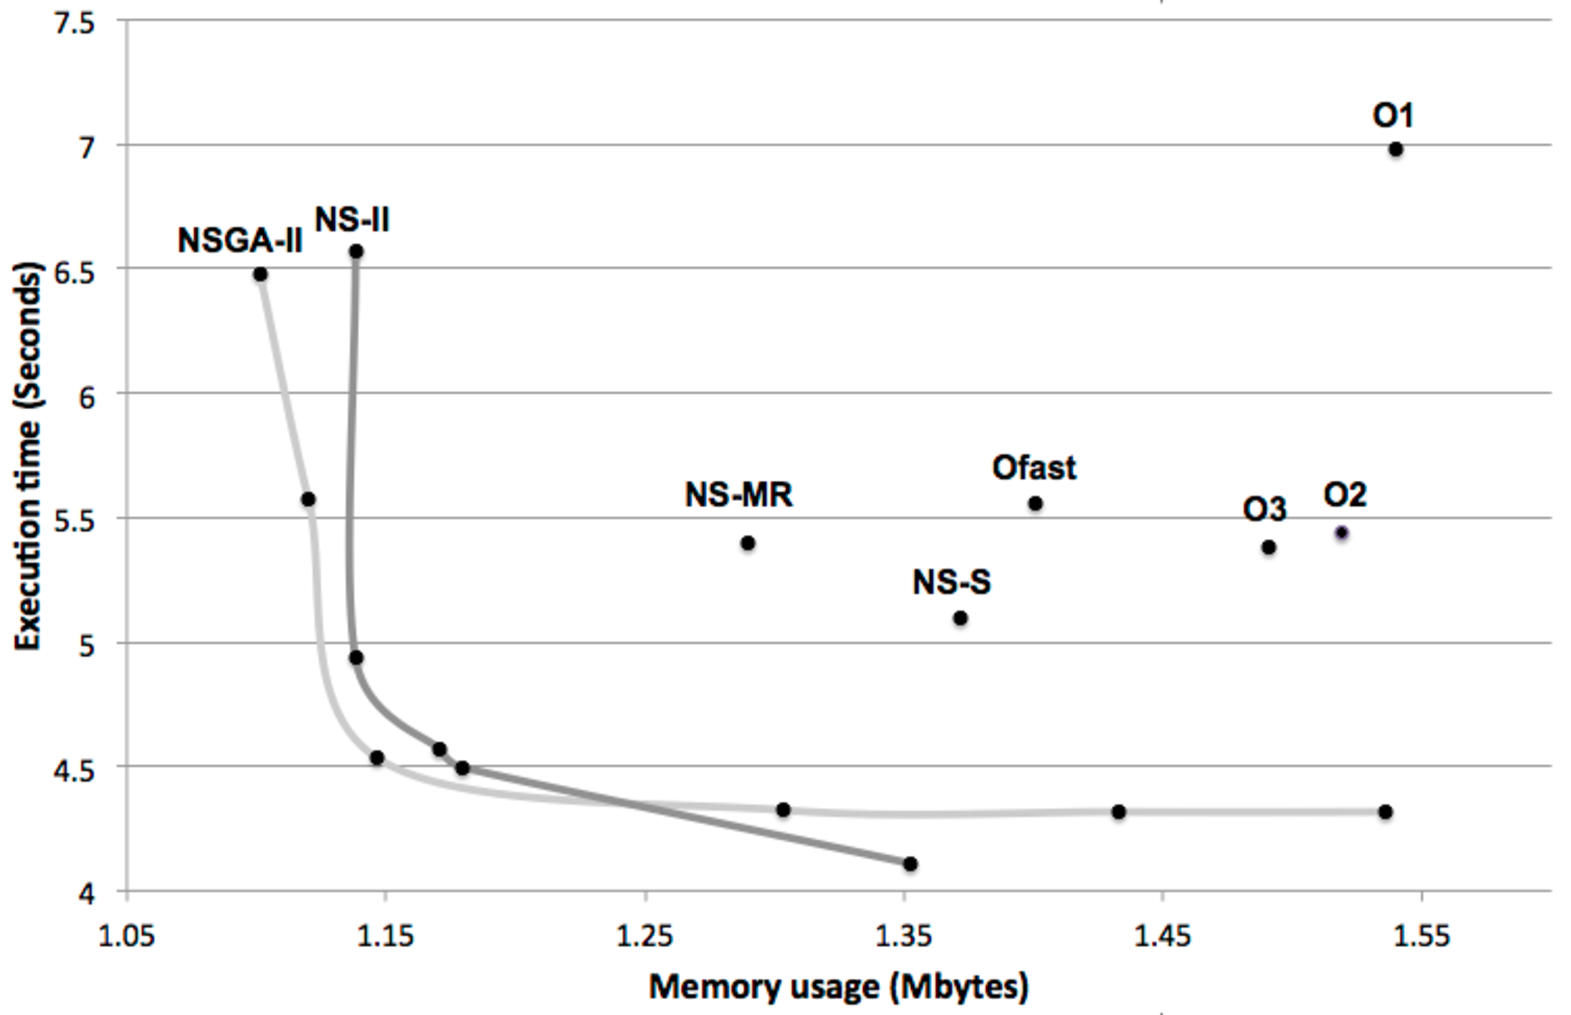
\includegraphics[width=0.9\linewidth]{chapitre3/fig/pareto.pdf}
		\caption{Comparison results of obtained Pareto fronts using NSGA-II and NS-II}
\end{figure}
	
	
\noindent\fbox{\parbox{\linewidth-2\fboxrule-2\fboxsep}{
			\textbf{Key findings for RQ4.} \\
			-- NOTICE is able to construct optimization levels that represent optimal trade-offs between non-functional properties. \\
			-- NS is more effective when it is applied for mono-objective search. \\
			-- NSGA-II performs better than our NS adaptation for multi-objective optimization. However, NS-II performs clearly better than standard GCC optimizations and previously discovered sequences in RQ1.
		}}
		
\subsection{Discussions}
Through these experiments, we showed that NOTICE is able to provide facilities to compiler users to test the non-functional properties of generated code. 

It provides also a support to search for the best optimization sequences through mono-objective and multi-objective search algorithms. NOTICE infrastructure has shown its capability and scalability to satisfy user requirements and key objectives in order to produce efficient code in terms of non-functional properties. 

During all experiments, standard optimization levels have been fairly outperformed by our different heuristics. 
Moreover, we have also shown (in RQ1 and RQ3) that optimizing for performance may be, in some cases, greedy in terms of resource usage. For example, the impact of standard optimization levels on resource usage is not always efficient even though it leads to performance improvement. 

Thus, compiler users can use NOTICE to evaluate the impact of optimizations on the non-functional properties and build their specific sequences by trying to find trade-offs among these non-functional properties (RQ4). 

We would notice that for RQ1, experiments take about 21 days to run all algorithms. This run time might seem long but, it should be noted that this search can be conducted only once, since in RQ2 we showed that best gathered optimizations can be used with unseen programs of the same category as the training set, used to generate optimizations. This has to be proved with other case studies. 

Multi-objective search as conducted in RQ4, takes about 48 hours, which we believe is acceptable for practical use. Nevertheless, speeding up the search speed may be an interesting feature for future research.
		
\subsection{Threats to Validity}
Any automated approach has limitations. We resume, in the following paragraphs, external and internal threats that can be raised:
		
\textit{External validity} refers to the generalizability of our findings. In this study, we perform experiments on random programs using Csmith and we use iterative compilation techniques to produce best optimization sequences. We believe that the use of Csmith programs as input programs is very relevant because compilers have been widely tested across Csmith programs~\cite{chen2016empirical,yang2011finding}. Csmith programs have been used only for functional testing, but not for non-functional testing. However, we cannot assert that the best discovered set of optimizations can be generalized to industrial applications since optimizations are highly dependent on input programs and on the target architecture. In fact, experiments conducted on RQ1 and RQ2 should be replicated to other case studies to confirm our findings; and build general optimization sequences from other representative training set programs chosen by compiler users.
		
\textit{Internal validity} is concerned with the causal relationship between the treatment and the outcome. Meta-heuristic algorithms are stochastic optimizers, they can provide different results for the same problem instance from one run to another. Are we providing a statistically sound method or it is just a random result? Due to time constraints, we run all experiments only once. Following the state-of-the-art approaches in iterative compilation, previous research efforts~\cite{hoste2008cole,martinez2014multi} did not provide statistical tests to prove the effectiveness of their approaches. This is because experiments are time-consuming. However, we can deal with these internal threats to validity by performing at least five independent simulation runs for each problem instance. 
		
		
\subsection{Tool Support Overview}
%TO ADD MAYBE
%Optimization options are difficult and even impossible to be chosen by programmers or compiler users.
%Therefore, a tool to help users to choose the best set of options becomes necessary to achieve a compiler optimization with effectiveness.


NOTICE provides also a GUI interface. The goal of this tool support is to help users to easily use NOTICE and finely auto-tune GCC compilers. This tool has been used to answer all previous research questions.

\begin{figure}[h]
	\center
	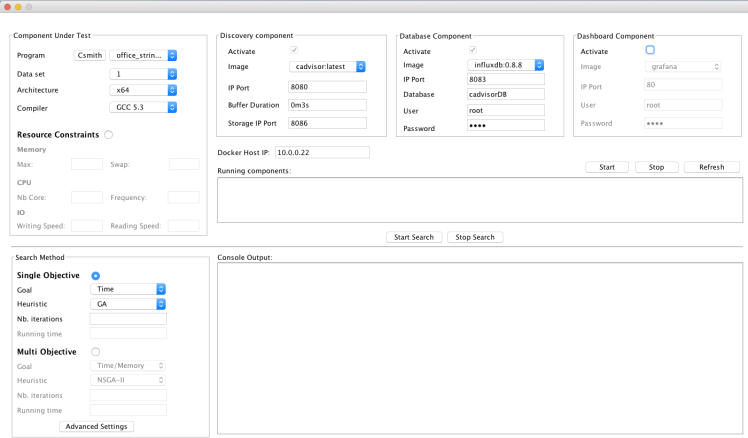
\includegraphics[scale=0.65]{chapitre3/fig/tool_support}
	\caption{Snapshot of NOTICE GUI interface}
	\label{fig:tool_support}
\end{figure}

For instance, NOTICE provides different features to help compiler users to:
\begin{itemize} 
	
	
	\item \textbf{Select the input program under test:} by generating a new Csmith program or by selecting an existing C program such as Cbench benchmark programs. The generation of a new Csmith program is done randomly.
	
	\item \textbf{Select datasets:} In case the selected program requires a dataset such as the case for Cbench programs, NOTICE allows the user to choose the dataset for the selected program. We recall that Cbench comes with a set of 20 datasets for each benchamrk program.
	
	\item \textbf{Select the target computer architecture:} choose the processor architecture where the experiments will be running such as x64, x86, ARM. This is part of our future work since we are running experiments only on native GCC compiler with x64 architecture. We are preparing a QEMU docker image to handle platforms heterogeneity.
	
	\item \textbf{Define the compiler version:} For now, NOTICE supports all GCC compiler versions from 3.x to 5.x. The process of extracting the target optimizations to evolve is done automatically (i.e., optimizations enabled by O1, O2, O3 and Ofast)
	
	\item \textbf{Configure the monitoring components:} This refers to the containers needed to extract all the information about the resource consumption. Configuring these components is possible with NOTICE such as image versions, labels, ports, logins, passwords.
	
	\item \textbf{Choose ip address of the cloud host machine:} NOTICE allows to run experiments remotely thanks to its micro-service infrastructure. Thus, we enable the user to select the ip of the remote machine.
	
	\item \textbf{Define resource constraints to running container:} In case we would run optimizations under resource constraints, it is possible to define memory and CPU constraints. By default, these option are disabled.
	
	\item \textbf{Choose the search method:} The user can select either a mono objective or multi-objective search.
	
	\item \textbf{Choose the meta-heuristic algorithm:} NOTICE supports GA, RS, and NS for mono objective search and NS, RS, and NSGA-II for multi-objective optimization.
 	
	\item \textbf{Choose the number of iterations:} The user can define the number of iterations for each algorithm which corresponds to the number of generated optimization sequences.

	\item \textbf{Choose the search time:} Instead of limiting the number of iterations, the user can fix a limit search time (in hours). 
	
	\item \textbf{Choose the optimization objective:} The goal can be reducing the execution time, memory, CPU, code size, or compilation time. For multi objective search, users can choose trade-offs between these objectives.
	
	\item \textbf{Edit evolutionary algorithm settings:} Tuning the evolutionary parameters (showed in Table 4.3) such as the population size, the novelty search settings, mutation and crossover probabilities, etc.
\end{itemize} 


The execution results of this tool (i.e., in the console output) will display at the end, the comparison results of standard optimization levels to the new discovered solutions.

\section{Conclusion}
%We present an automated approach for automatic extraction of non-functional properties of generated code.
Modern compilers come with huge number of optimizations, making complicated for compiler users to find best optimization sequences. Furthermore, auto-tuning compilers to meet user requirements is a difficult task since optimizations may depend on different properties (e.g., platform architecture, software programs, target compiler, optimization objective, etc.).

Hence, compiler users merely use standard optimization levels (O1, O2, O3 and Ofast) to enhance the code quality without taking too much care about the impact of optimizations on system resources.

In this chapter, we have introduced first a novel formulation of the compiler optimization problem based on Novelty Search. The idea of this approach is to drive the search for best optimizations toward novelty. 

Our work presents the first attempt to introduce diversity in iterative compilation. Experiments have shown that Novelty Search can be easily applied to mono and multi-objective search problems. 

In addition, we have reported the results of an empirical study of our approach compared to different state-of-the-art approaches, and the obtained results have provided evidence to support the claim that Novelty Search is able to generate effective optimizations.

Second, we have presented an automated tool for automatic extraction of non-functional properties of optimized code, called NOTICE. NOTICE applies different heuristics (including Novelty Search) and performs compiler auto-tuning through the monitoring of generated code in a controlled sand-boxing environment. In fact, NOTICE uses a set of micro-services to provide a fine-grained understanding of optimization effects on resource consumption. 

We evaluated the effectiveness of our approach by verifying the optimizations performed by GCC compiler. Then, we studied the impact of optimizations on memory consumption and execution time.

Results showed that our approach is able to automatically extract information about memory and CPU consumption. We were also able to find better optimization sequences than standard GCC optimization levels and construct optimizations that present optimal trade-offs between speedup and memory usage.






\chapter{A lightweight execution environment for automatic software testing and optimization}
\section{Introduction}

The general overview of the technical implementation is shown in Figure \ref{fig:docker_background2.pdf}. In the following subsections, we describe the deployment and testing architecture of generated code using system containers.


\begin{figure*}[!h]
	\center
	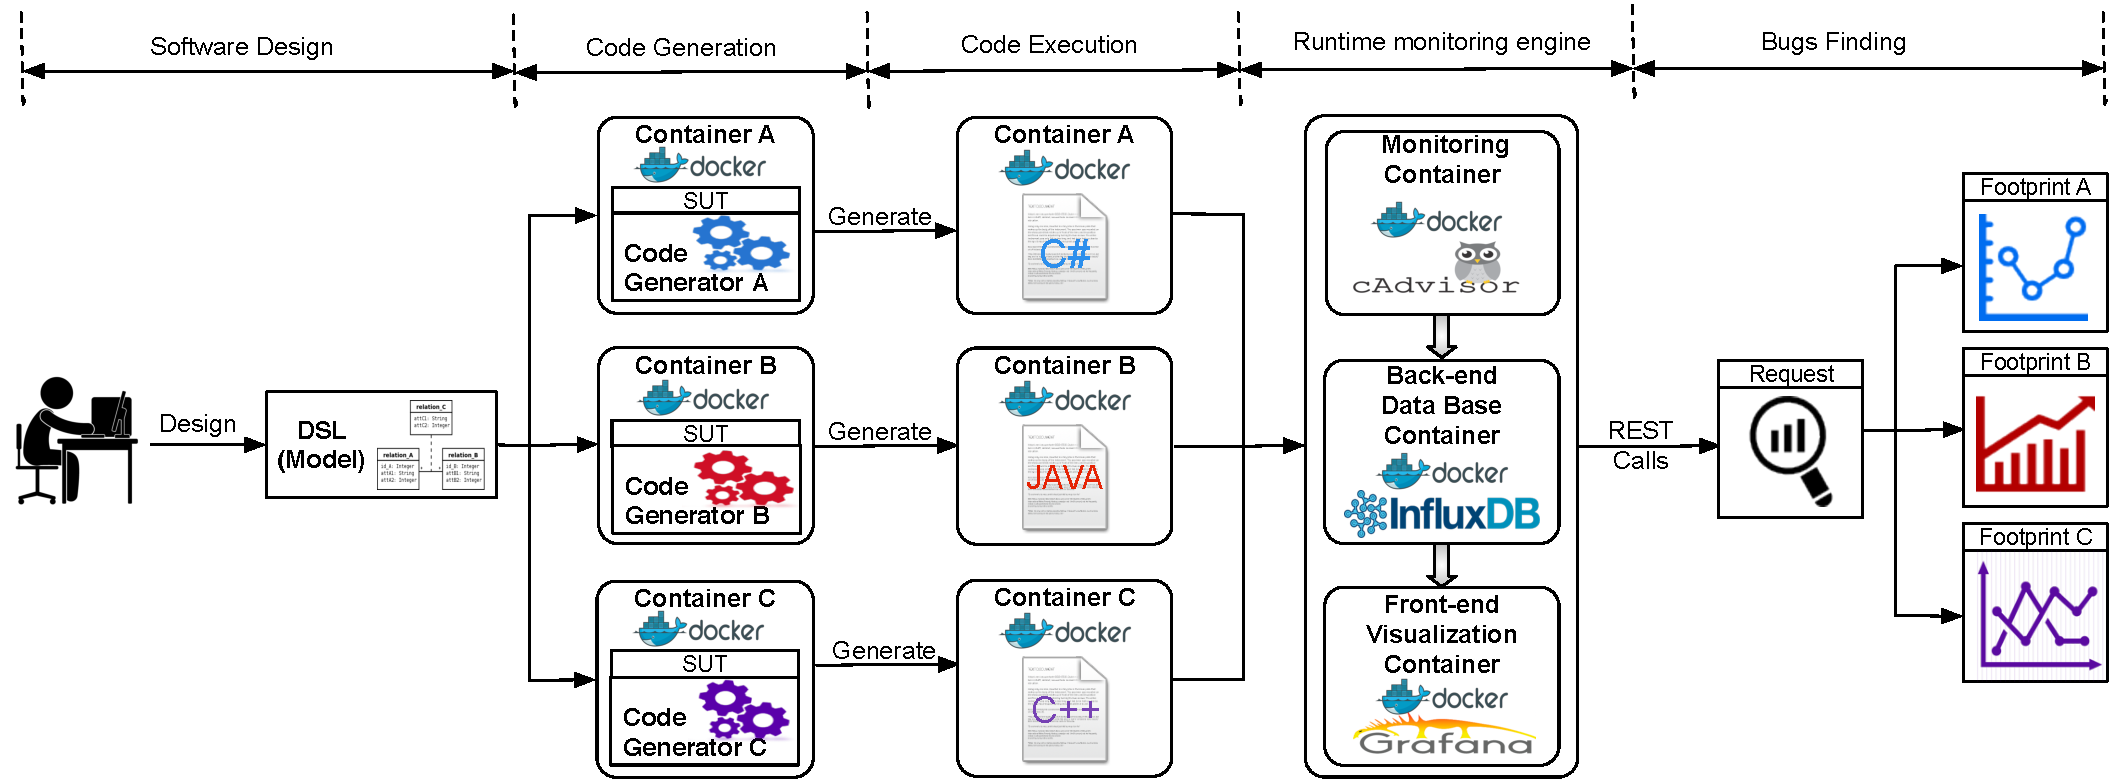
\includegraphics[width=0.95\linewidth]{chapitre5/fig/docker_background2.pdf}
	\caption{A technical overview of the different processes involved to ensure the code generation and non-functional testing of produced code from design time to runtime.}
	\label{fig:docker_background2.pdf}
\end{figure*}


\section{System Containers as Execution Platforms}


%For this purpose, we propose a testing infrastructure based on System Container techniques such as Docker\footnote{\url{https://www.docker.com}} environment. 
%This framework automates the deployment and execution of applications inside software containers by allowing multiple program configurations to run autonomously on different servers (i. e., a cloud servers).
%It also provides a distributed environment where system storage and resources can be finely managed and limited according to the needs. 

%Thus, we integrate a collection of components to define the adequate infrastructure for testing and monitoring of code generators. 


Before starting to monitor and test applications, we have to deploy generated code on different components to ease containers provisioning and profiling. 
We aim to use Docker Linux containers to monitor the execution of different generated artifacts in terms of resource usage~\cite{merkel2014docker}. 
Docker\footnote{\url{https://www.docker.com}} is an engine that automates the deployment of any application as a lightweight, portable, and self-sufficient container that runs virtually on a host machine. 
%To achieve that, Docker uses the Linux container technology. 
Using Docker, we can define pre-configured applications and servers to host as virtual images. We can also define the way the service should be deployed in the host machine using configuration files called Docker files. 
In fact, instead of configuring all code generators under test (GUTs) within the same host machine (as shown in Figure~1), our tool wrap each GUT within a container. To do so, we create a new configuration image for each GUT (i.e., the Docker image) where we install all the libraries, compilers, and dependencies needed to ensure the code generation and compilation. Thereby, the GUT produce code within multiple instances of preconfigured Docker images (see code generation step in Figure~2).
%As properties, we can define the OS where the service has to run, dependencies, etc. 
%A simple way to build images automatically is to use Dockerfiles which represents configuration files.
%Docker can build images automatically by reading the instructions from a Dockerfile. 
We use the public Docker registry\footnote{\url{https://hub.docker.com/}} for  saving, and managing all our Docker images. 
%It represents a cloud-based registry service for building and shipping application or service containers.
We can then instantiate different containers from these Docker images. 
%Basically, each container deploys an optimized version of the input source code program.

Next, each generated code is executed individually inside an isolated Linux container (see code execution step in Figure~2). By doing so, we ensure that each executed program runs in isolation without being affected by the host machine or any other processes. Moreover, since a container is cheap to create, we are able to create too many containers as long as we have new programs to execute.  
Since each program execution requires a new container to be created, it is crucial to remove and kill containers that have finished their job to eliminate the load on the system. We run the experiment on top of a private data-center that provide a bare-metal installation of  docker and docker swarm. On a single machine,  containers/softwares are running sequentially and we pin $p$ cores and $n$ Gbytes of memory for each container\footnote{$p$ and $n$ can be cofigured}. Once the execution is done, resources reserved for the container are automatically released to enable spawning next containers. Therefore, the host machine will not suffer too much from performance trade-offs.

In short, the main advantages of this approach are:
\begin{itemize}
	\item The use of containers induces less performance overhead and resource isolation compared to using a full stack virtualization solution~\cite{spoiala2016performance}. Indeed, instrumentation and monitoring tools for memory profiling like Valgrind~\cite{nethercote2007valgrind} can induce too much overhead.
	\item Thanks to the use of Dockerfiles, the proposed framework can be  configured by software testers in order to define the code generators under test (\eg, code generator version, dependencies, etc.), the host IP and OS, the DSL design, the optimization options, etc. Thus, we can use the same configured Docker image to execute different instances of generated code. For hardware architecture, containers share the same platform architecture as the host machine (e.g., x86, x64, ARM, etc.). 
	\item Docker uses Linux control groups (Cgroups) to group processes running in the container. This allows us to manage the resources of a group of processes, which is very valuable. 
	This approach increases the flexibility when we want to manage resources, since we can manage every group individually. For example, if we would evaluate the non-functional requirements of generated code within a resource-constraint environment, we can  request and limit resources within the execution container according to the needs.
	\item Although containers run in isolation, they can share data with the host machine and other running containers. Thus, non-functional data relative to resource consumption can be gathered and managed by other containers (\ie, for storage purpose, visualization)
\end{itemize}




\section{Runtime Testing Components}
In order to test our running applications within Docker containers, we aim to use a set of Docker components to ease the extraction of resource usage information (see runtime monitoring engine in Figure~2).
\subsection{Monitoring Component}
This container provides an understanding of the resource usage and performance characteristics of our running containers. Generally, Docker containers rely on Cgroups file systems to expose a lot of metrics about accumulated CPU cycles, memory, block I/O usage, etc. Therefore, our monitoring component automates the extraction of runtime performance metrics stored in Cgroups files. For example, we access live resource consumption of each container available at the Cgroups file system via stats found in \textit{"/sys/fs/cgroup/cpu/docker/(longid)/"} (for CPU consumption) and \textit{"/sys/fs/cgroup/memory/docker/(longid)/"} (for stats related to memory consumption). This component will automate the process of service discovery and metrics aggregation for each new container. Thus, instead of gathering manually metrics located in Cgroups file systems, it extracts automatically the runtime resource usage statistics relative to the running component (i.e., the generated code that is running within a container). We note that resource usage information is collected in raw data. This process may induce a little overhead because it does  very fine-grained accounting of resource usage on running container. Fortunately, this may not affect the gathered performance values since we run only one version of generated code within each container.
To ease the monitoring process, we integrate cAdvisor, a Container Advisor\footnote{\url{https://github.com/google/cadvisor}}. cAdvisor monitors service containers at runtime. 

However, cAdvisor monitors and aggregates live data over only 60 seconds interval. Therefore, we record all data over time, since container's creation, in a time-series database. It allows the code-generator testers to run queries and define non-functional metrics from historical data. Thereby, to make gathered data truly valuable for resource usage monitoring, we link our monitoring component to a back-end database component. 



\subsection{Back-end Database Component}
This component represents a time-series database back-end. It is plugged with the previously described monitoring component to save the non-functional data for long-term retention, analytics and visualization. 

During the execution of generated code, resource usage stats are continuously sent to this component. When a container is killed, we are able to access to its relative resource usage metrics through the database. We choose a time series database because we are collecting time series data that correspond to the resource utilization profiles of programs execution.

We use InfluxDB\footnote{\url{https://github.com/influxdata/influxdb}}, an open source distributed time-series database as a back-end to record data. InfluxDB allows the user to execute SQL-like queries on the database. For example, the following query reports the maximum memory usage of container $"generated\_code\_v1"$ since its creation:

\begin{lstlisting}[
language=SQL,
showspaces=false,
basicstyle=\small,
numberstyle=\small,
commentstyle=\color{gray},
linewidth=\columnwidth
]
select max (memory_usage) from stats 
where container_name='generated_code_v1'
\end{lstlisting}
To give an idea about the data gathered by the monitoring component and stored in the time-series database, we describe in Table \ref{tab:metrics} these collected metrics:
\begin{table}[h]
	\begin{center}
			\resizebox{0.8\columnwidth}{!}{%
		\begin{tabular}{|p{1.4cm}|p{6.6cm}|}
			\hline
			\textbf{Metric} & \textbf{Description} \\
				\hline
			Name & Container Name \\\hline
			
			T & Elapsed time since container's creation \\\hline
			
			Network  &  Stats for network bytes and packets in an out of the container \\\hline
			
			Disk IO &  Disk I/O stats \\\hline
			
			Memory  &  Memory usage \\\hline
			
			CPU &  CPU usage \\
			\hline
			
		\end{tabular}%
	}
		
	\end{center}
	\caption {Resource usage metrics recorded in InfluxDB}
	\label{tab:metrics}
\end{table}

Apart from that, our framework provides also information about the size of generated binaries and the compilation time needed to produce code.
For instance, resource usage statistics are collected and stored using these two components. It is relevant to show resource usage profiles of running programs overtime. To do so, we present a front-end visualization component for performance profiling. 

\subsection{Front-end Visualization Component}
%Once we gather and store resource usage data, the next step is visualizing them. That is the role of the visualization component. It will be the endpoint component that we use to visualize the recorded data. 
Once we gather and store resource usage data, the next step is visualizing them. That is the role of the visualization component. It will be the endpoint component that we use to visualize the recorded data. Therefore, we provide a dashboard to run queries and view different profiles of resource consumption of running components through web UI. Thereby, we can compare visually the profiles of resource consumption among containers. Moreover, we use this component to export the data currently being viewed into static CSV document. So, we can perform statistical analysis on this data to detect inconsistencies or performance anomalies (see bugs finding step in Figure~2).
%Moreover, we use this component to export the data currently being viewed into static CSV document. 
%Thereby, we can perform statistical analysis and process data to analyze performance behavior. 
%An overview of the monitoring dashboard is shown in Figure 3.
As a visualization component, we use Grafana\footnote{\url{https://github.com/grafana/grafana}}, a time-series visualization tool available for Docker. 


 	


\part{Conclusion and perspectives}
\chapter{Conclusion and perspectives}
In this chapter, we first summarize all the contributions of this thesis, recalling the challenges and how we addressed each of them. Next and finally, we discuss some perspectives for future work.

\section{Summary of contributions}
Generative software development has paved the way for the creation of multiple generators that serve as a basis for automatically generating code to a broad range of software and hardware platforms. With full automatic code generation, users are able to rapidly synthesize software artifacts for various software platforms. In addition, they can easily customize the generated code for the target hardware platform since modern generators (\ie, C compilers) become highly configurable, offering numerous configuration options that the user can apply. 
The quality of the automatically generated software is highly correlated to the configuration settings as well as the generator itself.
Therefore, we have highlighted, throughout this thesis, the challenges that we face when testing and auto-tuning generators. 

In reviewing the state of the art, we identified numerous approaches for testing generators. However, few of them evaluate the non-functional properties of automatically generated code, namely the performance and resource usage properties. The main issue we have identified when testing the non-functional properties is the oracle problem, since there is no a clear definition of how the oracle might be defined when it comes to the test of the performance and resource usage properties. Similarly, research in auto-tuning generators, especially compilers, has been studied for decades, proposing different solutions for exploring the large optimization search space. However, they  do not exploit the recent advances in search-based software engineering to effectively find the best configuration set. 
 
%in order to provide a new integrated software engineering approach which enables the advanced exploitation of the different dimensions of software diversity. 

From a software engineering point of view, this thesis contributes to improve the quality and reliability of generators. The contributions are summarized as follows: 

Our first contribution addresses the problem of non-functional testing of generators. In particular, we tackle the oracle problem in the domain of code generators testing. Thus, we propose an approach for automatically detecting inconsistencies in code generators in terms of non-functional properties (\ie, resource usage and performance).
Our approach is based on the intuition that a code generator is often a member of a family of code generators. Therefore, we benefit from the existence of multiple generators with comparable functionality (\ie, code generator families) to apply the idea of metamorphic testing~\cite{zhou2004metamorphic}, defining high-level test oracles (\ie, metamorphic relations) as test oracles. 
%To do so,  since we are comparing equivalent implementations of the same program written in different languages, we assume that the memory usage and execution time should be more or less the same with a small variation for each test suite across the different versions.
We define the metamorphic relation as a comparison between the variations of performance and resource usage of code, generated from the same code generator family. Any variation that exceeds a specific threshold value is automatically detected as an anomaly. We apply two statistical methods (\ie, principal component analysis and range-charts) in order to automate the inconsistencies detection.
We evaluate our approach by analyzing the performance of Haxe, a popular high-level programming language that involves a set of cross-platform code generators. We evaluate the properties related to the resource usage and performance for five different target software platforms. 
We run a bench of test suites across 7 Haxe benchmark libraries in order to verify the metamorphic relation (\ie, the performance and memory usage variation) for each of them. Experimental results show that our approach is able to detect, among 95 executed test suites, 11 performance and 15 memory usage inconsistencies, violating the metamorphic relation . These results show that our approach can automatically detect real issues in code generator families.

The second contribution addresses the problem of generators auto-tuning. Particularly, we are interested in auto-tuning compilers because of the large number of configuration options (i.e., optimizations) they offer to control the quality of the generated code. In this context, we exploit the recent advances in search-based software engineering in order to provide an effective approach to tune compilers (i.e., through optimizations) according to user's non-functional requirements (i.e., performance and resource usage). Our approach, called NOTICE, applies a novel formulation, compared to previous related work, of the compiler
optimization problem using the Novelty Search algorithm\cite{lehman2008exploiting}. Novelty Search is applied to tackle the
problem of optimizations diversity and then, providing a new way to explore the huge optimization search space. In fact, since the search
space of possible combinations is multi-modal\cite{bodin1998iterative} and too large, we apply this technique is to explore the search space of possible compiler optimization options by considering sequence diversity as a single objective.
We conduct an empirical study to evaluate the effectiveness of our approach by verifying the optimizations performed by the GCC compiler. Our experimental results show that NOTICE is able to auto-tune compilers according to user choices (heuristics, objectives, programs, etc.) and construct optimizations that yield to better performance results than standard optimization levels and classical genetic algorithms. We also demonstrate that NOTICE can be used to automatically construct optimization levels that represent optimal trade-offs between the speedup and memory usage using multi-objective algorithms.

Evaluating the resource usage of automatically generated code is complex because of the diversity of software and hardware platforms that exist in the market. To handle this problem, we present in the third contribution the technical details of the infrastructure used to collect the non-functional metrics (e.g., memory and CPU consumptions) of automatically generated code (by either compilers or code generators). In fact, we benefit from the recent advances in lightweight system virtualization, in particular container-based virtualization, in order to offer effective support for automatically deploying, executing, and monitoring the generated code in heterogeneous environment.
The same monitoring infrastructure is used to evaluate the experiments conducted in the two first contributions.

\section{Perspectives}
The work presented in this thesis represents a step towards proving support to evaluate generators. In the reminder of this chapter we will describe possible improvements and extensions to the contributions of this thesis.

\paragraph{Tracking the source of code generator inconsistencies} 
In Chapter \ref{chap:code generators}, we present a black-box testing approach that identifies the presence of potential issues within code generator families. However, we do not provide detailed information about the source of the issues. We investigated the generated code manually in order to fix the bug. As a future work, we believe that a traceability method can be applied to collect and visualize information about the inconsistency, at the source code level. Thus, we can help code generator maintainers to easily identify the source of the bugs (\eg, code snippets that affect the the software performance), and fixing the issues.

\paragraph{Improving the efficiency of our auto-tuning approach}
We plan to explore more trade-offs among resource usage metrics \eg, the correlation between CPU consumption and speedup. Using the Docker technology, we can run containers easily on different host machines in the cloud. As a future work, we want to evaluate our approach across different hardware architectures.
We also intend to provide more facilities to NOTICE users in order to test optimizations performed by modern compilers such as Clang, LLVM, etc.
Finally, NOTICE can be easily adapted and integrated to new case studies. As an example, we would inspect the behavior of code generators since different optimizations can be performed to generate code from models~\cite{stuermer2007systematic}. The same approach can be applied as long as the code generator accept many configuration options.

\paragraph{Speed up the time required to tune and test generators}
Throughout the experiments conducted in this thesis, we use to run containers sequentially. This can take too much time, especially when configuring compilers the tuning time grows exponentially as long as we have new configurations to evaluate. 
In order to reduce the time needed to run and monitor multiple versions of generated code (e.g., optimized versions), we intend to deploy tests on many nodes in the cloud using multiple containers in parallel. Doing so, we will be able to accelerate the testing process. Solutions as Docker Swarm already exist and can be applied to manage clusters of containers running in parallel in the cloud.













%----------------------------------------------------------------------
% END MATERIAL
%----------------------------------------------------------------------

% B I B L I O G R A P H Y
% -----------------------

% The following statement selects the style to use for references.  It controls the sort order of the entries in the bibliography and also the formatting for the in-text labels.
\bibliographystyle{alpha}
% This specifies the location of the file containing the bibliographic information.  
% It assumes you're using BibTeX (if not, why not?).
\cleardoublepage % This is needed if the book class is used, to place the anchor in the correct page,
                 % because the bibliography will start on its own page.
                 % Use \clearpage instead if the document class uses the "oneside" argument
\phantomsection  % With hyperref package, enables hyperlinking from the table of contents to bibliography             
% The following statement causes the title "References" to be used for the bibliography section:
\renewcommand*{\bibname}{References}

% Add the References to the Table of Contents
\addcontentsline{toc}{chapter}{\textbf{References}}


\bibliography{uw-ethesis}
% Tip 5: You can create multiple .bib files to organize your references. 
% Just list them all in the \bibliogaphy command, separated by commas (no spaces).

% The following statement causes the specified references to be added to the bibliography% even if they were not 
% cited in the text. The asterisk is a wildcard that causes all entries in the bibliographic database to be included (optional).
\nocite{*}

\newpage
\cleardoublepage
\phantomsection \label{listoffigs}
\addcontentsline{toc}{chapter}{List of Figures}
\markboth{List of Figures}{List of Figures}
\listoffigures

\newpage
\phantomsection \label{listoftabs}
\addcontentsline{toc}{chapter}{List of Tables}
\markboth{List of Tables}{List of Tables}
\listoftables


\end{document}
